\documentclass[12pt, a4paper, twoside, openright]{book}

\usepackage{vuwthesis} % sets up some local things, mostly the front page

\usepackage{palatino} % sets palatino as the default font

\usepackage{url} % for typesetting urls

\usepackage[version=3]{mhchem}		%Chemical formula i.e. /ce
\usepackage{color}					%For using different colour formats
\usepackage{siunitx} 				%SI units package
\usepackage{booktabs}				%For making tables pretty
\usepackage[floats=float]{chemscheme}	%Scheme environment
\usepackage{nicefrac}				%For nice fractions
\usepackage{graphicx}				%Required to set figure widths
\usepackage{mciteplus}
\usepackage{achemso}
\usepackage{hyperref}
\usepackage[xindy]{glossaries}

\newfloat{structure}{hbp}{lox}[chapter]

%%%%%%%%%%%%%%%%%%%%%%%%%%%%%%%%%%%%%%%%%%%%%%%%%%%%%%%
%NEW COMMANDS GO HERE%

% Misc. Commands
\newcommand{\sub}[1]{$_{\mbox{#1}}$}
\newcommand{\fixme}[1]{\colorbox[rgb]{1,0.5,0}{\textbf{#1}}}
\newcommand{\textprime}{$\textquoteright$}
\newcommand{\textsubscript}[1]{$_{\mbox{#1}}$}  % Required to get it to compile remove at the end

\newcommand{\percm}{\fixme{PER CM}}

% Shortcuts for degrees and degrees C
\newcommand{\degC}{\mbox{$\,^\circ$C}}
\newcommand{\degrees}{$^\circ$}

% Shortcuts for pKa and pKb
\newcommand{\pKa}{p\emph{K}\textsubscript{a}}
\newcommand{\pKb}{p\emph{K}\textsubscript{b}}

% Shortcuts for NMR intros
\newcommand{\Protonintro}[2]{\proton{} NMR (#1 MHz, \ce{#2}): $\delta{}$}
\newcommand{\Phosphorusintro}[1]{\phosphorus{} NMR (121 MHz, \ce{#1}): $\delta{}$}
\newcommand{\Carbonintro}[2]{\carbon{} NMR (#1 MHz, \ce{#2}): $\delta{}$}
\newcommand{\Fluorineintro}[1]{\fluorine{} NMR (282 MHz, \ce{#1}): $\delta{}$}

% Shortcuts for 1H, 10B, 11B, 13C, 19F, 31P, 77Se, 107Ag, 109Ag and 195Pt
\newcommand{\proton}{\ce{^{1}H}}
\newcommand{\Bten}{${^{10}}$B}
\newcommand{\Beleven}{${^{11}}$B}
\newcommand{\carbon}{\ce{^{13}C}}
\newcommand{\fluorine}{\ce{^{19}F}}
\newcommand{\phosphorus}{\ce{^{31}P}}
\newcommand{\selenium}{\ce{^{77}Se}}
\newcommand{\Agseven}{${^{107}}$Ag}
\newcommand{\Agnine}{${^{109}\mbox{Ag}}$}
\newcommand{\Pt}{\ce{^{195}Pt}}

%Shortcut for J, 1J and 2J
\newcommand{\J}{\mbox{\emph{J}}}
\newcommand{\oneJ}{\mbox{\textsuperscript{1}\emph{J}}}
\newcommand{\twoJ}{\mbox{\textsuperscript{2}\emph{J}}}

% Shortcut for 1JCH etc.
\newcommand{\oneJCH}{\mbox{\textsuperscript{1}\emph{J}\textsubscript{CH}}}
\newcommand{\oneJNH}{\mbox{\textsuperscript{1}\emph{J}\textsubscript{NH}}}
\newcommand{\oneJXH}{\mbox{\textsuperscript{1}\emph{J}\textsubscript{XH}}}
\newcommand{\oneJPtP}{\mbox{\textsuperscript{1}\emph{J}\textsubscript{PtP}}}
\newcommand{\oneJPtC}{\mbox{\textsuperscript{1}\emph{J}\textsubscript{PtC}}}
\newcommand{\oneJPM}{\mbox{\textsuperscript{1}\emph{J}\textsubscript{PM}}}
\newcommand{\JPSe}{\mbox{\textsuperscript{1}\emph{J}\textsubscript{PSe}}}
\newcommand{\JHH}{\mbox{\emph{J}\textsubscript{HH}}}
\newcommand{\JPH}{\mbox{\emph{J}\textsubscript{PH}}}
\newcommand{\JPC}{\mbox{\emph{J}\textsubscript{PC}}}
\newcommand{\JPF}{\mbox{\emph{J}\textsubscript{PC}}}
\newcommand{\JPtP}{\mbox{\emph{J}\textsubscript{PtP}}}
\newcommand{\JRhP}{\mbox{\emph{J}\textsubscript{RhP}}}
\newcommand{\JRhC}{\mbox{\emph{J}\textsubscript{RhC}}}
\newcommand{\JPtH}{\mbox{\emph{J}\textsubscript{PtH}}}
\newcommand{\JPtC}{\mbox{\emph{J}\textsubscript{PtC}}}
\newcommand{\JPP}{\mbox{\emph{J}\textsubscript{PP}}}
\newcommand{\JCF}{\mbox{\emph{J}\textsubscript{CF}}}
\newcommand{\JPtF}{\mbox{\emph{J}\textsubscript{PtF}}}
\newcommand{\JAgP}{\mbox{$^1\textit{J}$\textsubscript{AgP}}}
\newcommand{\JAgPseven}{\mbox{$^1\textit{J}$\textsubscript{$^{107}$AgP}}}
\newcommand{\JAgPnine}{\mbox{$^1\textit{J}$\textsubscript{$^{109}$AgP}}}
\newcommand{\twoJPtH}{\mbox{\textsuperscript{2}\emph{J}\textsubscript{PtP}}}

% Shortcuts for NMR data
\newcommand{\NMRPC}[4]{#1 (#2, \JPC{}~=~#3~Hz, #4)}  % C1 (C2, \JPC{}~=~C3~Hz)
\newcommand{\NMRAgP}[3]{#1 (d, \JAgPseven{}~=~#2~Hz, d, \JAgPnine{}~=~#3~Hz)}
\newcommand{\NMRPH}[4]{#1 (#2, \JPH{}~=~#3~Hz, #4)} 
\newcommand{\NMRPPt}[2]{#1 (s, \JPtP{}~=~#2~Hz)}
\newcommand{\NMRPtwoPt}[4]{#1 (#2, \JPtP{}~=~#3~Hz, #4)}
\newcommand{\NMRPtH}[5]{#1 (#2, \textsuperscript{#3}\JPtH{}~=~#4~Hz, #5)}
\newcommand{\NMRPtC}[5]{#1 (#2, \textsuperscript{#3}\JPtC{}~=~#4~Hz, #5)}
\newcommand{\NMRHH}[4]{#1 (#2, #3~Hz, #4)} 
\newcommand{\NMRCF}[4]{#1 (#2, \JCF{}~=~#3~Hz, #4)} 
\newcommand{\NMRPF}[4]{#1 (#2, \JPF{}~=~#3~Hz, #4)} 
\newcommand{\NMRbsinglet}[2]{#1 (bs, #2)}
\newcommand{\NMRsinglet}[2]{#1 (s, #2)}
\newcommand{\NMRcoupled}[4]{#1 (#2, \J{}~=~#3~Hz, #4)} 
\newcommand{\NMRPsinglet}[1]{#1 (s)}
\newcommand{\NMRmultiplet}[2]{#1 (m, #2)}
\newcommand{\NMRdd}[4]{#1 (dd, #2, #3~Hz, #4)}
\newcommand{\NMRobscuredH}[4]{#1 (obscured, assigned by #2 correlation, #3, #4)}
\newcommand{\NMRobscuredC}[3]{#1 (obscured, assigned by #2 correlation, #3)}

%\renewcommand{\baselinestretch}{1.00}

%!TEX root = Thesis.tex

\newacronym{CFC}{CFC}{chlorofluorocarbon}
\newacronym{dmpe}{dmpe}{1,2-bis(dimethylphosphino)ethane}
\newacronym{mesitylene}{mesitylene}{1,3,5-trimethylbenzene}
\newacronym{hemimellitene}{hemimellitene}{1,2,3-trimethylbenzene}
\newacronym{durene}{durene}{1,2,4,5-tetramethylbenzene}
\newacronym{bpym}{bpym}{2,2$'$-dipyrimidine}
\newacronym{oleum}{oleum}{sulfur trioxide in concentrated sulfuric acid}
\newacronym{cod}{cod}{1,5-cyclooctadiene}
\newacronym{Cy}{Cy}{cyclohexyl}
\newacronym{py}{py}{pyridyl}
\newacronym{dbf}{dbf}{dibenzofuran}
\newacronym{TOF}{TOF}{turnover frequency}
\newacronym{DMSO}{DMSO}{dimethylsulfoxide}
\newacronym{cymene}{cymene}{1-methyl-4-(1-methylethyl)benzene}
\newacronym{xantphos}{xantphos}{4,5-bis(diphenylphosphino)-9,9-dimethylxanthene}
\newacronym{DPEphos}{DPEphos}{bis(2- diphenylphosphinophenyl)ether}
\newacronym{dppe}{dppe}{1,2-(diphenylphosphino)ethane}
\newacronym{TMEDA}{TMEDA}{N,N,N',N'-tetramethyl-ethane-1,2-diamine}
\newacronym{cot}{cot}{1,3,5-cyclooctatriene}
\makeglossaries

\begin{document}

\frontmatter
% Book style knows about front matter
% Report style doesn't so you need to set roman numbering etc yourself :-(

%%%%%%%%%%%%%%%%%%%%%%%%%%%%%%%%%%%%%%%%%%%%%%%%%%%%%%%

\title{Late Transition Metal Complexes of POP Pincer Ligands}
\author{Melanie R. M. Nelson}

\subject{Chemistry}
\abstract{An abstract of fewer than 500 words must be included.}
% Books don't normally have abstracts, and this is a bit of a hack

% Uncomment the appropriate degree
\phd
%\mscthesisonly
%\mscwithhonours
%\mscbothparts
% \otherdegree{DEGREE OR DIPLOMA NAME}



%%%%%%%%%%%%%%%%%%%%%%%%%%%%%%%%%%%%%%%%%%%%%%%%%%%%%%%




\maketitle

%!TEX root = Thesis.tex

\chapter*{Acknowledgements}
\label{ch:acknowledgements}

As always there are numerous people that have helped me over the years.  My supervisor, Prof. John Spencer, thank you for your guidance, advice and support, even coming in to University after a major earthquake to rescue our reaction. Dr. Matthias Lein, thank you for being an excellent supervisor while John was on research and study leave and for all of your assistance with DFT.  Thanks to both of you for reading through various sections while on holiday.

The past and present members of the JLS research group: Almas, Brad, Chris, David, Kathryn, Lia, Rosie, Sarah and Teresa.  Thank you for getting excited with me over the minutiae of NMR spectra, and for all of the good times and commiserations that we've shared.  The other postgraduate students in SCPS, particularly my office mates in AM204, thanks for your friendship over the years.

The general staff of SCPS are amazingly supportive towards the research in the school and many things would be impossible without them.  Particular thanks to the lab technicians Teresa, Jamie-Ann and Jackie, for letting me borrow glassware and other equipment.  Thanks to Peter Northcote, Ian Vorster and John Ryan for helping with NMR.  I am grateful to Rob Keyzers and Yinrong Lu for help with mass spectrometry and to Jan Wikaira, Christ Fitchett and Matt Polson at the 	University of Canterbury for X-ray crystallography.  

Thank you to the members of Disarray, and all of my non-chemistry friends for giving me something else to think about when I just needed a break.  My family have been extremely supportive and caring, as they always are.  Finally to my husband, Stephen, these last 10 years have been wonderful, thank you for all of your love and understanding especially over these last few months.

I would also like to acknowledge Victoria University of Wellington for funding through the PhD, submission, and Curtis-Gordon scholarships.  
%
%\begin{itemize}
%\item{John and Matthias}
%\item{Lab techs, Teresa, Jamie, Shekira, Jackie}
%\item{NMR, Peter, Ian, John Ryan}
%\item{Mass spec, Rob, Ian, Yinrong}
%\item{Crystallography, Jan, Chris, Matt?}
%\item{Lab group, Rosie, Sarah, Teresa, Kathryn, Brad, Chris, David, Almas}
%\item{Stephen}
%\end{itemize}

\tableofcontents
\printglossaries

%%%%%%%%%%%%%%%%%%%%%%%%%%%%%%%%%%%%%%%%%%%%%%%%%%%%%%%

% book style knows about mainmatter
% if you are using report style you will have to rest page numbering etc.
\mainmatter

%%%%%%%%%%%%%%%%%%%%%%%%%%%%%%%%%%%%%%%%%%%%%%%%%%%%%%%

% individual chapters included here

%!TEX root = Thesis.tex

\chapter{Introduction}
\label{chapter:introduction}

Diphosphine ligands are one of the cornerstones of transition metal coordination chemistry.  Their ability to control the steric and electronic environment around the metal centre imparts control over the reactivity patterns of the complexes.  This thesis provides an account of research into the synthesis, properties and coordination chemistry of three diphosphine ligands with bulky \tBu{} substituents and a rigid backbone, resulting in a large bite-angle.  

%\fixme{Stephen wants to fix this with me, re-write with research objectives in mind.}

\section{Tertiary Phosphine Ligands}

Tertiary phosphine ligands are some of the most ubiquitous in coordination chemistry.  Phosphines coordinate to transition metals by donation of the lone pair on the phosphorus atom forming a $\sigma$-bond and $\pi$-back-donation in the P-C anti-bonding $\sigma^*$ orbitals which have $\pi$ symmetry.\cite{Orpen1990}  This combination forms stable coordination complexes with a range of different transition metals and oxidation states.  The strong coordination of phosphine ligands means they are not readily displaced in a catalytic process, resulting in increased lifetimes of the catalytic species and consequently higher \glspl{TON}.  The array of different phosphine ligands available allows control over the steric and electronic properties that are imparted to the metal centre resulting in  improved selectivity or activity in different catalytic systems.  As such, phosphine ligands have been used as ancillary ligands in a wide range of different catalytic processes including industrial-scale processes.\cite{Noyori2002, Nicolaou2005, Knowles2002}

\subsection{Electronic and Steric Properties}

Altering the groups coordinated to the phosphorus atom in tertiary phosphine ligands can have a significant impact on the electronic and steric properties of the phosphine.  As the nature of the metal is controlled largely by the coordinated ligands, several studies have quantified the electronic and steric properties of phosphine ligands.  \cite{Tolman1977, Banger2009, Dunne1991, Roodt2003, Mann1980, Tiburcio2006, Tolman1970}  

Most investigations of electronic properties involve the measurement of the carbonyl stretching frequency in a metal carbonyl complex such as [Ni\ce{(CO)3L}], [Mo\ce{(CO)5L}] or [Rh(CO)Cl\ce{L2}]\footnote{The nomenclature used in this thesis is in accordance with the Nomenclature of Inorganic Chemistry - IUPAC Recommendations 2005.\cite{IUPAC2005}}\cite{Tolman1977, Tolman1970, Roodt2003, Banger2009}  If a spin active nucleus such as rhodium or platinum is used, then the value of the one-bond metal-phosphorus coupling constant can also offer insight into the electronic properties of the phosphine ligand\cite{Mann1980, Pregosin2012, Roodt2003, Banger2009}  The value of the one-bond phosphorus-selenium coupling constant in a phosphinoselenide has been used as a way to study the electronic properties of phosphines.\cite{Beckmann2011, Allman1982}  The phosphinoselenides are readily synthesised, air-stable solids which avoid the need for transition metals or the use of toxic gases.  A comparison of the different techniques used to measure the electronic properties has shown good correlation between the various series.\cite{Banger2009}

%The electronic properties can be investigated in a number of different ways.  However, the most typical way involves the synthesis of a metal complex which has an easily measured parameter.  The first investigation into these properties was performed by synthesising a series of nickel(0) carbonyl complexes of the type \ce{[Ni(CO)3L]}\footnote{The nomenclature used in this thesis is based on the Nomenclature of Inorganic Chemistry - IUPAC Recommendations 2005.\cite{IUPAC2005}}   and determining the carbonyl stretching frequency.\cite{Tolman1977}  The carbonyl stretching frequency is highly dependent on the electronic properties of the metal centre which is controlled by the ancillary ligands.  Carbonyl ligands are strong $\pi$-acceptor ligands and coordinate to the metal \emph{via} donation from a $\sigma$ orbital and back donation into the $\pi^*$ anti-bonding orbital of the \ce{C#O} bond.  As this is an anti-bonding orbital, additional electron density decreased the C-O bond order and thus the observed stretching frequency is reduced.  As such, phosphines with strongly electron donating substituents such as alkyl groups result in a large reduction in the stretching frequency while phosphines with electron withdrawing substituents such as aryl groups have a smaller shift.   In some unusual cases with very strongly electron withdrawing substituents on the phosphorus centre the \ce{C#O} stretch can be shifted to higher wave numbers than that reported for free, uncoordinated carbon monoxide (2143 \si{\per\cm}).\cite{Anderson2014}

%A number of other related approaches have been utilised in the literature to analyse the electronic properties of tertiary phosphines.  The C-O stretching frequency in the octahedral \ce{[Mo(CO)5L]} complex and square planar \ce{Rh(CO)ClL2]} complex have been used to further investigate the electronic influence of phosphines on the metal centre.\cite{Banger2009}  The series correlate well though the specific values vary as the metals also have different electronic character.   Typically the values for the Tolman nickel series are from 2056.1-2110.8 \si{\per\cm} (\ce{PtBu3, PF3}) for the nickel series, 2066-2104 \si{\per\cm} (\ce{P(o-Tol)3}, \ce{P(CF3)3}) for the molybdenum series and 1943-2016 \si{\per\cm} (\ce{PCy3}, \ce{P(OPh)3}) for the rhodium complexes.  In general alkyl substituents like Me, Et, \fixme{iPr}, \tBu{} and cyclohexyl donate more electron density than phenyl substituents and phosphite ligands (bonding to phosphorus through an oxygen).  Fluorophosphines and fluoroalkylsubstituted phosphines are most commonly the least electron donating as the strong electron negativity of the fluorine atoms withdraws electron density from the phosphorus, making the lone pair less available for coordination to the metal.  

%One point of interest with the rhodium complexes is that as there are two phosphorus atoms coordinated to the rhodium this gives the possibility of \cis{} or \trans{} isomers.  The most commonly reported isomer \fixme{check this} is the \trans{} isomer, although the technique has also been used to study \cis{} complexes of diphosphine ligands.  This indicates the sensitivity of using carbonyl ligands as a probe for the electronic properties as, generally the strongest effect is felt for ligands in a \trans{} position (c.f \trans{} influence and \trans{} effect).
%
%The values for the rhodium complexes are typically shifted further to lower wave numbers than the values for the nickel and the molybdenum series.  This is expected as rhodium is a late transition-metal and thus more electron rich than the mid-series molybdenum and the first-row nickel.  The Tolman series of \ce{[Ni(CO)3L]} complexes is the most well-known and henceforth has the largest number of reported values in the literature, both the molybdenum and rhodium series have been shown to correlate well with the nickel series.  

%\Gls{NMR} spectroscopy has also been used to investigate the electronic properties of phosphine ligands.  \phosphorus{} \gls{NMR} is a very sensitive technique, and can be used to probe complexes which may be too unstable to obtain an infrared spectrum.   A further advantage is that the probe for the electronic properties in this case is a phosphorus-atom coupling constant.  Thus the phosphorus is directly incorporated into the probe meaning that it can give a better understanding of the phosphorus directly rather than an overview of many potential synergistic effects.  The previously mentioned \ce{[Rh(CO)Cl(L)2]} complexes and \trans-\ce{[PtCl2L2]} have been used to investigate the electronic properties of various phosphine ligands.  Rhodium-103 and platinum-195 both have spins of 1/2 meaning that they couple to the coordinated phosphorus atoms.  While \ce{^{103}Rh} is 100\% abundant, \Pt{} is only 34\% abundant with the other isotopes not spin active.  Hence the \phosphorus{} \gls{NMR} spectrum in \ce{[Rh(CO)Cl(L)2]} appears as a doublet while in \trans-\ce{[PtCl2L2]} a singlet with \Pt{} satellites is observed.  The coupling constants for \ce{[Rh(CO)Cl(L)2]} range from 114.7 - 193.9 Hz for \ce{PMe3} to \ce{POMe3} with most values falling between 114.7 and 142.3 Hz.  For \trans-\ce{[PtCl2L2]} the values range from 2379 Hz for the electron rich \ce{PMe3} and 5694 Hz for the electron poor, \ce{P(OEt)3} with most  of the values between 2379 and 3145 Hz.  The values vary greatly between the metals as platinum has a greater gyromagnetic ratio than rhodium.\cite{Pregosin2012}  However, the trends are consistent between the series.  Coupling constants are influenced by the amount of s-character that a given bond has.  Generally the more s-character the higher the coupling constant for that bond.  According to Bent's rule ``atomic s-character concentrates in orbitals directed towards electropositive substituents''.  Thus the greater the metal-phosphorus coupling constant the more s-character is present in the M-P bond, thus indicating a greater degree of electronegative substituents, and thus the less electron donating the phosphine ligand will be.  In this case we see that the lower coupling constants are found for the trialkyl phosphines while the higher coupling constants are found for the tri(fluoroalkyl)phosphines and phosphinites.  

%Although phosphines are typically studied for their use as ligands in transition metal complexes, it is possible to investigate their electronic properties without using metals.  Phosphines react readily with chalcogens resulting in oxidation of the phosphorus to a P(V) species.  These molecules are generally easily synthesised and air-stable solids.  Selenium has a number of different isotopes with mass numbers 76, 77, 78, 80 and 82.  All of these have a nuclear spin of zero except \ce{^{77}Se} with a spin of -1/2.  \ce{^{77}Se} is only 7.6\% abundant, thus the \phosphorus{} \gls{NMR} signal appears as a singlet with selenium satellite.  The phosphine selenides show coupling constants of 673 - 805 Hz, though some higher values have been observed.  Again these rely on the changing s-character resulting from the different electronegativities of the phosphorus atom's substituents.  The more electronegative the substituents are, the more s-character will be in the phosphorus selenium bond, thus resulting in a higher coupling constant.  The trend is the same as previous examples whereby the trialkyl phosphines have the lowest coupling constants indicating an electron rich phosphorus.  The phenyl substituted phosphines have higher coupling constants indicating their less electron rich nature.  The fluoro substituted phosphines, phosphinites and phosphites have much higher coupling constants indicating their electron withdrawing character.  

The steric properties of different ligands have also been examined from a quantitative perspective.  The Tolman cone angle is the angle formed at the apex of a cone centred at 2.28 \si{\angstrom} from the phosphorus atom where the outer edges of the cone lie at the Van der Waals radii of the outer most atom of the ligand.  The Tolman cone angle has some limitations: it was originally determined using physical molecular models with idealised bond lengths and Van der Waals radii which do not take into account the changes that may occur in actual molecules.  In addition, the Tolman cone angle is a maximum cone angle which works well for approximately symmetrical spherical substituents such as \ce{PMe3} or \ce{PtBu3}, however when planar rings, such as phenyl substituents, are present these can rotate readily, resulting in much larger changes to the cone angle than a trialkyl phosphine would exhibit.  The Tolman cone angles for aryl systems tends to be larger than the crystallographically determined cone angle.

%As expected we see that the largest cone angles are for the \ce{P(mesityl)3,} \ce{P(o-Tol)3}, \ce{P(C6F5)3}, \ce{PtBu3} and \ce{P(neopentyl)3} with values of 212, 194, 184, 182 and 180\degrees.  These ligands all have a significant steric impact on the phosphorus and thus will reduce the available space around a transition metal in a coordination complex.   The smallest cone angles are for \ce{P(NCH2CH2)3}, \ce{P(OEt)3} and \ce{P(OCH2CH2Cl)3} with values of 108, 109 and 110\degrees{} respectively.  The smallest phosphine with non-heteroatom substituents is \ce{PMe3} with a cone angle of 118\degrees.  The other common trialkyl phosphines (\ce{P(Et)3}, \ce{P(Bu)3} and \ce{P(Pr)3}) all have a cone angle of 132\degrees indicating that beyond an ethyl group further increases in change length has little impact.  Branching of the chain does have an impact however, with \ce{P(i-Bu)3}, \ce{P(iPr)3}, \ce{P(sec-Bu)3} and \ce{P(tBu)3} having cone angles of 143, 160, 160 and 182 respectively indicating that branching has a significant impact.  

%===========================================================================
\subsection{Diphosphine Ligands}

Diphosphine ligands consist of two tertiary phosphines linked by a backbone.  A selection of diphosphine ligands are shown in Figure \ref{diphosphineligands}.  Most commonly, the backbone is a carbon skeleton such as an ethyl, propyl, or xylyl group as found in \acrshort{dppe}, \acrshort{dppp}, or \acrshort{dbpx}.  Larger groups can also be used as backbones, such as the binapthyl ligand \acrshort{BINAP}, or the \acrshort{BISBI} system.  The backbones can also include heteroatoms such as \acrshort{diop} or \acrshort{DPEphos}, or transition metal as in the ferrocene molecule found in \acrshort{dppf}.  The backbone can also be used to produce chiral ligands including \acrshort{BINAP}, \acrshort{diop} or \acrshort{SEGphos}, which can be used for asymmetric catalysis.\cite{Noyori2002, Agbossou1995, Shimizu2007}  Diphosphine ligands typically chelate to transition metals, resulting in enhanced stability through the chelate effect.  The chelate effect is an entropic effect, in the presence of a free-coordination site on a complex with a non-chelating diphosphine ligand the coordination of the other phosphorus atom will be faster than the coordination of another ligand.\cite{Housecroft2005}  In mono-phosphine complexes, the mono-phosphine must compete with the other components in the mixture as there is no entropic driver for a second molecule of the mono-phosphine to coordinate over any other ligands in the system.  Hence the increased thermodynamic stability of complexes with bidentate chelating ligands compared to the same complex with analogous monodentate ligands.  

\begin{figure}[htbp]
\centering
\begin{subfigure}[b]{0.3\textwidth}
	\centering
	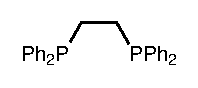
\includegraphics{../Figures/Diphosphines/dppe.eps}
	\caption{dppe}
	\label{dppe}
\end{subfigure}
~
\begin{subfigure}[b]{0.3\textwidth}
	\centering
	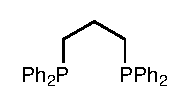
\includegraphics{../Figures/Diphosphines/dppp.eps}
	\caption{dppp}
	\label{dppp}
\end{subfigure}
~
\begin{subfigure}[b]{0.3\textwidth}
	\centering
	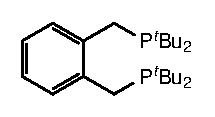
\includegraphics{../Figures/Diphosphines/dbpx.eps}
	\caption{dbpx}
	\label{dbpx}
\end{subfigure}
\\
\vspace{0.5cm}
\begin{subfigure}[b]{0.3\textwidth}
	\centering
	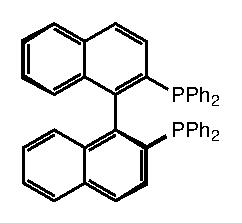
\includegraphics{../Figures/Diphosphines/BINAP.eps}
	\caption{BINAP}
	\label{BINAP}
\end{subfigure}
~
\begin{subfigure}[b]{0.3\textwidth}
	\centering
	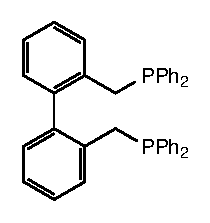
\includegraphics{../Figures/Diphosphines/BISBI.eps}
	\caption{BISBI}
	\label{BISBI}
\end{subfigure}
~
\begin{subfigure}[b]{0.3\textwidth}
	\centering
	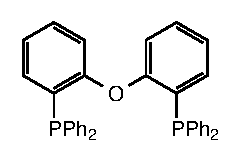
\includegraphics{../Figures/Xantphosderivatives/DPEphos.eps}
	\caption{DPEphos}
	\label{DPEphos}
\end{subfigure}
\\
\vspace{0.5cm}
\begin{subfigure}[b]{0.3\textwidth}
	\centering
	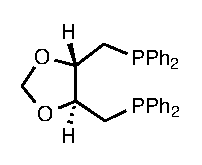
\includegraphics{../Figures/Diphosphines/DIOP.eps}
	\caption{diop}
	\label{diop}
\end{subfigure}
~
\begin{subfigure}[b]{0.3\textwidth}
	\centering
	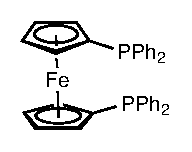
\includegraphics{../Figures/Diphosphines/dppf.eps}
	\caption{dppf}
	\label{dppf}
\end{subfigure}
~
\begin{subfigure}[b]{0.3\textwidth}
	\centering
	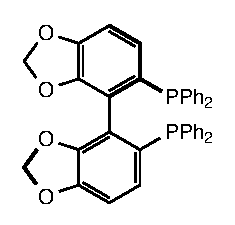
\includegraphics{../Figures/Diphosphines/SEGphos.eps}
	\caption{SEGphos}
	\label{SEGphos}
\end{subfigure}
\\
\caption[Selection of diphosphine ligands]{Selection of diphosphine ligands.}
\label{diphosphineligands}
\end{figure}

The electronic and steric properties of diphosphines ligands can be described using the techniques developed for mono-phosphines.\cite{Tolman1977, Banger2009, Dunne1991, Roodt2003, Mann1980, Tiburcio2006, Tolman1970}  The bite-angle defined as the P-M-P angle in a transition-metal complex (Figure \ref{Biteangle}) can also be used to quantify and compare different diphosphine ligands.  The natural bite-angle is defined as the P-Rh-P angle calculated by molecular modelling using a rhodium atom with fixed Rh-P distances of 2.315 \si{\angstrom}.\cite{Casey1990}  The bite-angle for a given complex can also be measured from an X-ray crystal structure.  The original development of the natural bite-angle parameter included a comparison of the natural and crystallographic bite-angles for seven different complexes, showing good correlation between the natural and crystallographic bite-angles.\cite{Casey1990}  Further study in 1999 showed that, for a range of different diphosphine ligands, the crystallographic bite-angles occur within a very narrow range which correlate well with the natural bite-angles.\cite{Dierkes1999}

\begin{figure}[ht]
\centering
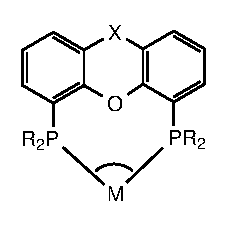
\includegraphics[]{../Figures/Biteangle.eps}
\caption[The bite angle]{The bite angle}
\label{Biteangle}
\end{figure}

When used as ancillary ligands in transition metal catalysts, diphosphines can result in different product distributions compared with the analogous monophosphines.  The catalytic reaction of ethene and carbon monoxide, in a methanol solution, produced short chain oligiomers when [Pd(MeCN\ce{)4](BF4)2} was used with an excess of a monophosphine ligand such as triphenylphosphine.\cite{Lai1984}  Changing to a stoichiometric amount of a chelating diphosphine with a [Pd(OAc\ce{)2]} precursor, results in the co-polymerisation of carbon monoxide and ethene giving polyketone indicating that the rate of chain termination is faster for mono-phosphine complexes than in the diphosphine complexes.\cite{Drent1991}  The bite-angle of the diphosphine was shown to have a significant impact on the rate of the reaction.  When performed with the \ce{Ph2(CH2)_{n}PPh2} (n = 1 - 6) series of ligands, the highest rate was observed for \gls{dppp} (n = 3) with values decreasing as the chain length was increased or decreased.\cite{Drent1991}  The steric bulk of the ligands is also important, changing the phenyl substituents on \acrshort{dppp} for \tBu{} groups resulted in high selectivity for the mono-insertion product methyl propionate.\cite{Leeuwenbook2000}  Introducing further rigidity to the system by changing to the xylene backbone ligand \gls{dbpx} resulted in methyl propionate exclusively.\cite{Eastham2000}

%===========================================================================
\subsection{Wide Bite-Angle Diphosphine Ligands}

The bite-angle of diphosphine ligands can have a significant impact on their reactivity.  Ligands with bite-angles around 90\degrees{} will typically coordinate in a \cis{} geometry in square-planar and octahedral complexes and occupy axial-equatorial positions in trigonal bipyramidal complexes.  Ligands with larger natural bite-angles closer to 120\degrees{} can coordinate in a bis-equatorial arrangement in the trigonal bipyramidal complexes.\cite{Kranenburg1995}  Two of the most important catalytic steps are oxidative addition and reductive elimination, which result in changes to the coordination number and geometry of the metal centres.\cite{Tsuji1995}  Altering the bite-angles of the ancillary ligands can have a significant impact, typically with larger bite-angle ligands favouring reductive elimination steps.\cite{Freixa2003}  The strain on ligands to coordinate with bite-angles significantly different to their natural bite-angle, can result in destabilisation of particular intermediates in catalytic cycles leading to increased selectivity.\cite{Freixa2003}  A wide-range of diphosphine ligands with large bite-angles have been reported, including, dbpx, BISBI, DBFphos and \Phxantphos{} (Figures, \ref{dbpx}, \ref{BISBI}, \ref{widebiteanglediphosphines}).  Diphosphines with extremely large bite-angles, designed to coordinate in an exclusively \trans{} geometry in square-planar complexes have been reported such as, TRANSphos, SPANphos, and norphos (Figure \ref{transdiphosphines})\cite{Freixa2003b, Kamer2001, Dierkes1999}.

\begin{figure}[htbp]
\centering
\begin{subfigure}[b]{0.3\textwidth}
	\centering
	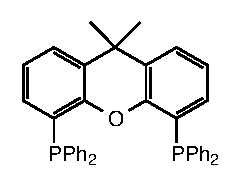
\includegraphics{../Figures/Xantphosderivatives/Phxantphos.eps}
	\caption{\Phxantphos}
	\label{biteanglePhxantphos}
\end{subfigure}
~
\begin{subfigure}[b]{0.3\textwidth}
	\centering
	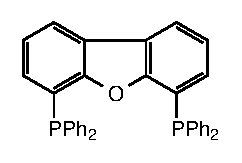
\includegraphics{../Figures/Xantphosderivatives/DBFphos.eps}
	\caption{DBFphos}
	\label{biteangleDBFphos}
\end{subfigure}
\caption[Wide bite-angle diphosphine ligands]{Wide bite-angle diphosphine ligands.}
\label{widebiteanglediphosphines}
\end{figure}

\begin{figure}[htbp]
\centering
\begin{subfigure}[b]{0.3\textwidth}
	\centering
	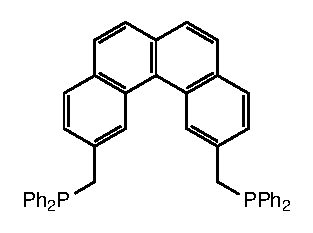
\includegraphics{../Figures/Diphosphines/TRANSphos.eps}
	\caption{TRANSphos}
	\label{TRANSphos}
\end{subfigure}
~~~
\begin{subfigure}[b]{0.3\textwidth}
	\centering
	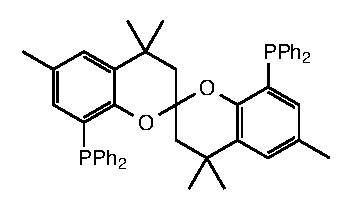
\includegraphics{../Figures/Diphosphines/SPANphos.eps}
	\caption{SPANphos}
	\label{SPANphos}
\end{subfigure}
~~~
\begin{subfigure}[b]{0.3\textwidth}
	\centering
	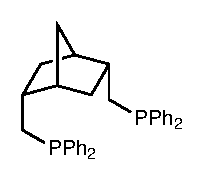
\includegraphics{../Figures/Diphosphines/norphos.eps}
	\caption{norphos}
	\label{norphos}
\end{subfigure}
\caption[Trans-spanning diphosphine ligands]{Selected trans-spanning diphosphine ligands.}
\label{transdiphosphines}
\end{figure}

%===========================================================================
\section{Pincer Ligands}

Diphosphine ligands such as \Phxantphos{} with wide bite-angles and a heteroatom in the centre of the backbone have the potential to act as pincer ligands.  Pincer ligands have attracted research attention due to their unique balance of stability and reactivity.\cite{Becerra2009}  Pincer ligands are tridentate ligands that coordinate to transition-metals in an exclusively meridional fashion.\cite{Choi2011}   The ligands are typically named according to their donor atoms, such as PCP, PNP, POP or NCN.  If the groups between the donor atoms contain heteroatoms then these may be included in the naming also, for example POCOP.  The pincer ligands may be anionic (as with PCP ligands) or neutral (PNP and POP).\cite{Vlugt2009, Kataoka1995}  Although phosphines are the most common donor groups, amines,\cite{Singleton2003} imines,\cite{Takenaka2005} thioethers\cite{Zim2000} and N-heterocyclic carbenes\cite{Hahn2007} have all been reported.

\begin{figure}[ht]
\centering
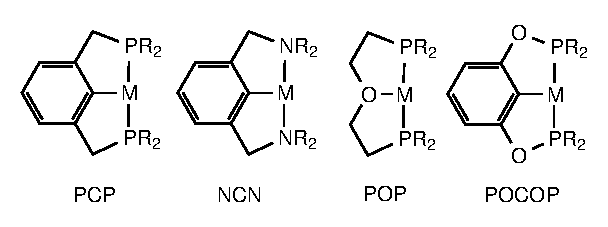
\includegraphics[]{../Figures/Pincernaming.eps}
\caption[Naming of pincer ligands]{Naming of pincer ligands}
\label{Pincernaming}
\end{figure}

Pincer ligands were first reported in 1976 by Shaw and Alcock.\cite{Moulton1976, Alcock1976}  Shaw reported a \emph{tert}-butyl PCP ligand (Figure \ref{ShawPCP}) and introduced the naming scheme that has become commonplace for pincer ligands.  When reacted with an appropriate metal precursor, complexes formed between the tridentate ligand with nickel, palladium, platinum, rhodium, and iridium with chloride, nitrile, hydride, and carbon monoxide ligands.\cite{Moulton1976}  Alcock reported the first POP pincer ligands together with their rhodium carbonyl complexes, characterised by X-ray crystallography (Figure \ref{AlcockPOP}).\cite{Alcock1976}  

\begin{figure}[htbp]
\centering
\begin{subfigure}[b]{0.3\textwidth}
	\centering
	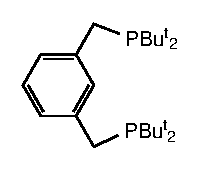
\includegraphics{../Figures/Shaw.eps}
	\caption{}
	\label{ShawPCP}
\end{subfigure}
~
\begin{subfigure}[b]{0.3\textwidth}
	\centering
	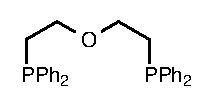
\includegraphics{../Figures/Alcock.eps}
	\caption{}
	\label{AlcockPOP}
\end{subfigure}
\\
\caption[First reported pincer ligands]{First reported pincer ligands.}
\label{Pincerligands}
\end{figure}

The different components of pincer ligands have significant influence on the steric and electronic properties and hence their reactivity.\cite{Singleton2003}  Altering the central donor group, X (Figure \ref{Pincerligands}) can lead to changes in electronic effects. mostly through the \trans{}-influence.\cite{Choi2011}  For example, a carbon donor ligand has a greater \trans{}-influence than an oxygen donor.  Thus ligands \trans{} to X in PXP complexes will be bound more strongly when X~=~O than X~=~C.\cite{Zhu2008} The donor group Y controls the steric environment around the metal centre and the electron density.  Changing the backbone and other remote groups gives control over the electron density on the metal and can be used to improve solubility properties.\cite{Choi2011}

\begin{figure}[htbp]
\centering
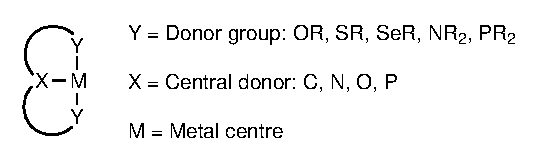
\includegraphics{../Figures/Pincerligands.eps}
\caption[General representation of pincer ligands]{General representation of pincer ligands}
\label{Pincerligands}
\end{figure}

The tridentate coordination of pincer ligands, typically forming two five-membered metallacycles, imparts significant stability to metal complexes with pincer ligands.\cite{Choi2011}  The stability of the complexes is such that the backbone can undergo functionalisation at the 4-position to trimethylsilane \emph{via} lithiation with \emph{tert}-butyllithium and treatment with trimethylchlorosilane, without inducing any decomposition of the platinum complex (Scheme \ref{Stability}).\cite{Albrecht2001}  This inherent stability allows the complexes to act as catalysts for highly endothermic reactions that require high temperatures, such as alkane dehydrogenation.\cite{Choi2011}

\begin{scheme}[htbp]
\centering
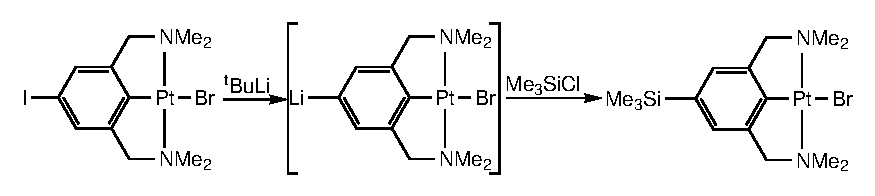
\includegraphics[]{../Schemes/Stability.eps}
\caption[Functionalisation of an NCN pincer ligand]{Functionalisation of an NCN pincer ligand}
\label{Stability}
\end{scheme}

Coordination complexes of pincer ligands have a large number of applications.  Platinum complexes of an NCN pincer ligand have been utilised as sensors for the detection of sulfur dioxide.\cite{Albrecht2000, Albrecht2000c, Albrecht2001}  Palladium and nickel complexes of a number of pincer ligands have shown activity in cross-coupling reactions.\cite{Hahn2007, Bedford2000, Kimura2006, Zim2000, Obora2006} Theoretical studies have shown potential uses for pincer ligands in water-splitting\cite{Sandhya2011} and nitrogen fixation.\cite{Holscher2007}  However, one of the most prominent uses of pincer ligands is the activation of C-H bonds, typically as dehydrogenation catalysts.\cite{Choi2011, Albrecht2001, Crabtree2001}

%===========================================================================
\section{Xantphos}

First reported in 1995 by van Leeuwen et al., the \acrshort{xantphos}\footnote{The term xantphos is used in the literature to mean either the general class of ligands or the specific ligand 9,9-dimethyl-4,6-bis(diphenylphosphino)xanthene.  For the purposes of this thesis the specific ligand will be referred to as \Phxantphos{} and the term xantphos will be used to represent a generic ligand from this class.} class of diphosphine ligands were designed to investigate the influence of the bite angle on catalytic reactions, in particular rhodium catalysed hydroformylation.\cite{Kranenburg1995}  The general structure and a selection of different xantphos derivatives are given in Figure \ref{xantphosderivatives}.  The first paper on xantphos included derivatives where the \ce{CMe2} group in the backbone of \Phxantphos{} (Figure \ref{Phxantphos}) was replaced by a S (\Phthixantphos, Figure \ref{Phthixantphos}), \ce{SiMe2} (\Phsixantphos, Figure \ref{Phsixantphos}), a direct bond between the atoms, or removed entirely (DPEphos, Figure \ref{DPEphos}).  Since then an vast array of derivatives have been reported.  The most common position for derivatisation is the bridgehead position (occupied by a \ce{CMe2} group in \Phxantphos{}).  Changes to this position can create subtle bite-angle changes while only resulting in minor electronic changes. Other derivatives have changed the substituents on the phosphorus atoms including cyclic groups, chiral derivatives or changes for solubility.  The phosphorus donors have also been replaced with a range of different groups including phosphonites, amines, imines, arsines, and thioethers.\cite{Veen2000b, Malaise2006, Goertz1998, Haaren2002} The third site for derivatisation is the position, \emph{meta} to the phosphorus atoms on the backbone phenyl rings.  In \Phxantphos{} this position is occupied by protons, while in \Phthixantphos{} methyl groups are present.  Derivatives with \tBu{} or sulfate groups have also been reported.\cite{Goedheijt1998, Goedheijt1998b, Veen1999}\footnote{In the literature two different structures are commonly referred to as  \tBuxantphos{}, one with \tBu{} substituents on the aromatic backbone and one with \tBu{} groups on the phosphorus atoms.  For the purpose of this thesis the structure with the \tBu{} substituents on the phosphorus will be named \tBuxantphos{} and the structure with the \tBu{} groups on the aromatic backbone will be named \emph{t}-Bu-(\Phxantphos).}  These alterations all result in changes to the bite-angle of the ligand.  

\begin{figure}[htbp]
\centering
\begin{subfigure}[b]{0.35\textwidth}
	\centering
	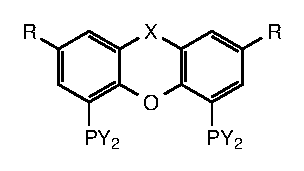
\includegraphics{../Figures/Xantphosderivatives/Generic.eps}
	\caption{General structure}
	\label{genericxantphos}
\end{subfigure}
~
\begin{subfigure}[b]{0.3\textwidth}
	\centering
	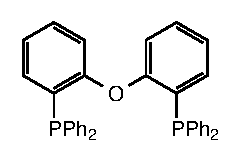
\includegraphics{../Figures/Xantphosderivatives/DPEphos.eps}
	\caption{DPEphos, 102\degrees}
	\label{DPEphos}
\end{subfigure}
~
\begin{subfigure}[b]{0.3\textwidth}
	\centering
	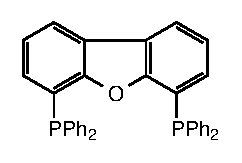
\includegraphics{../Figures/Xantphosderivatives/DBFphos.eps}
	\caption{DBFphos, 131\degrees}
	\label{DBFphos}
\end{subfigure}
\\
\vspace{0.5cm}
\begin{subfigure}[b]{0.35\textwidth}
	\centering
	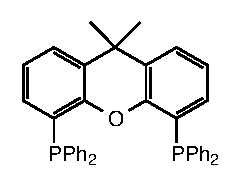
\includegraphics{../Figures/Xantphosderivatives/Phxantphos.eps}
	\caption{\Phxantphos, 111\degrees}
	\label{Phxantphos}
\end{subfigure}
~
\begin{subfigure}[b]{0.3\textwidth}
	\centering
	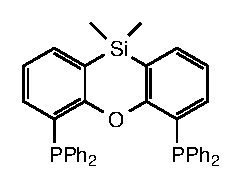
\includegraphics{../Figures/Xantphosderivatives/Sixantphos.eps}
	\caption{\Phsixantphos, 108\degrees}
	\label{Phsixantphos}
\end{subfigure}
~
\begin{subfigure}[b]{0.3\textwidth}
	\centering
	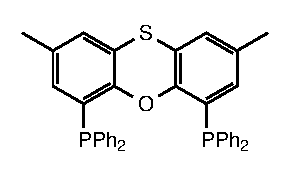
\includegraphics{../Figures/Xantphosderivatives/Phthixantphos.eps}
	\caption{\Phthixantphos, 110\degrees}
	\label{Phthixantphos}
\end{subfigure}
\\
\vspace{0.5cm}
\begin{subfigure}[b]{0.35\textwidth}
	\centering
	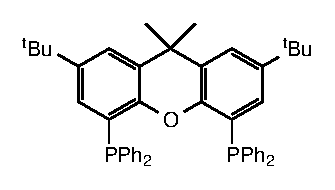
\includegraphics{../Figures/Xantphosderivatives/tBu-Phxantphos.eps}
	\caption{tBu-\Phxantphos, 110\degrees}
	\label{tBuPhxantphos}
\end{subfigure}
~
\begin{subfigure}[b]{0.3\textwidth}
	\centering
	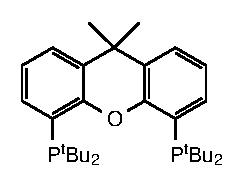
\includegraphics{../Figures/Xantphosderivatives/tBu-xantphos.eps}
	\caption{\tBuxantphos, 140\degrees}
	\label{tBuxantphos}
\end{subfigure}
~
\begin{subfigure}[b]{0.3\textwidth}
	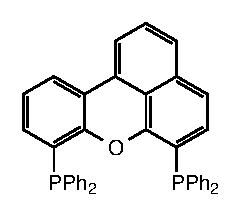
\includegraphics{../Figures/Xantphosderivatives/Benzoxantphos.eps}
	\caption{Benzoxantphos, 120.6\degrees}
	\label{Benzoxantphos}
\end{subfigure}
\\
\vspace{0.5cm}
\begin{subfigure}[b]{0.35\textwidth}
	\centering
	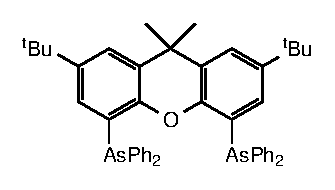
\includegraphics{../Figures/Xantphosderivatives/Xantarsine.eps}
	\caption{Xantarsine, 113\degrees}
	\label{Xantarsine}
\end{subfigure}
~
\begin{subfigure}[b]{0.6\textwidth}
	\centering
	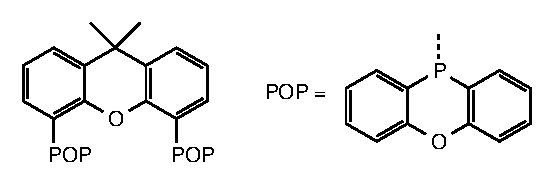
\includegraphics{../Figures/Xantphosderivatives/POP-xantphos.eps}
	\caption{POP-xantphos, 123\degrees}
	\label{POP-xantphos}
\end{subfigure}
\\
\caption[Selection of xantphos derivatives]{Selection of xantphos derivatives with their natural bite-angles (where known).\cite{Dierkes1999, Veen1999, Veen2000, Veen2000b}}
\label{xantphosderivatives}
\end{figure}

The influence of the bite-angle of diphosphine ligands on the selectivity and activity of their transition metal complexes in various catalytic process has been investigated using the xantphos ligands.  The hydroformylation of alkenes to give branched and linear aldehydes is an industrially important reaction with the linear aldehydes typically of higher industrial importance.\cite{Leeuwenbook2000}  In the hydroformylation of 1-octene using various xantphos ligands, a linear correlation between the natural bite-angle of the diphosphine and the percentage of produced linear aldehyde was observed.\cite{Kranenburg1995}  From this and other kinetics studies, the bite-angle has been determined to have both a steric and electronic component.\cite{Veen1998, Leeuwen2000}  The hydride-migration step determines the regioselectivity of the reaction.  In this case additional steric crowding of the metal centre, resulting from a larger bite-angle, can lead to favouring of the less sterically demanding transition state - that which produces the linear aldehyde.\cite{Freixa2003}  Carrying out the hydroformylation of styrene or 1-octene with a series of thixantphos complexes where the phenyl substituents on the phosphorus atoms were substituted in the \emph{para}-position with various electron donating or electron withdrawing substituents, showed differences in the \glspl{TOF} of the reaction.\cite{Veen1998}  This is thought to be related changes in the metal hybridisation, changing the reactivity of the metal towards reductive elimination.\cite{Slot2002, Freixa2003}

The xantphos ligands were the first phosphine ligands to form active hydrocyanation catalysts on nickel.\cite{Kranenburg1995b}  Using styrene as a substrate, diphosphines with alkyl backbones, such as \gls{dppe}, \gls{dppp} and \gls{dppb} showed little product (\textless{}10\%) while the xantphos ligands gave yields ranging from 27-95\%, with the highest for \Phsixantphos{}.  Ligands with bite-angles close to 105\degrees{} resulted in higher yields and selectivities whilst decreasing the bite angle to 101\degrees{} or increasing to 110\degrees{} led to a much lower activity.  The bite angle is thought to influence the reaction by stabilising preferred reaction intermediates and destabilising inactive species.   In the hydrocyanation reaction a bite angle close to 109\degrees{} destabilises square-planar Ni(II) species and stabilises the tetrahedral Ni(0) species, enhancing the reductive elimination step and resulting in a faster reaction.\cite{Goertz1998}  The increased rate of reactivity of xantphos complexes compared to \gls{dppp}, \gls{BINAP}, \gls{dppf}, and \gls{DPEphos} has also been observed in a range of different cross-coupling reactions.\cite{Birkholz2009}

A search of the \gls{CSD} indicates that of the crystallographically determined structures, most complexes with xantphos derivatives involve bidentate \dento{}P,P\textprime{} coordination.\cite{Allen2002}  Four 2-coordinate complexes have been reported, all coordinated to gold. Ten 3-coordinate structures have been published.  With 4-coordinate metals, tetrahedral complexes are the most common (31 structures), followed by pseudo-\trans{} square-planar complexes (26), then \cis{} square-planar geometries (20).  This is particularly interesting as the bite-angle for the xantphos complexes is closer to a 90\degrees{} than to 180\degrees.  On pentacoordinate metals 10 complexes have been reported with one square-pyramidal structure, three axial-equatorial, and six bis-equatorial trigonal bipyramidal complexes found.  Six different octahedral complexes have been reported, all with the xantphos ligand occupying a \cis{}-geometry.  The xantphos ligands can also coordinate in a \POP{} geometry in addition to the bidentate \dento{}P,P\textprime{} mode.  This \POP{} coordination is more common than the \dento{}P,P\textprime{} in octahedral complexes with 24 reported.  However, it is much less common in five coordinate complexes with only four \POP{} complexes and 10 \POP{} four-coordinate complexes.  A monodentate \dento{}P bonding mode is also possible, though it is very rare, with only one crystal structure reported to date.\cite{Escalle2009}

\fixme{For the above, do I need to cite the actual papers or is citing the CSD enough?}

Given the possibility of \POP{} and \dento{}P,P\textprime{} coordination the xantphos ligands also have the potential for hemilability of the central donor group whereby the oxygen can bind reversibly to the metal centre in order to stabilise catalytic intermediates. This has been utilised in the hydroacylation of alkenes and alkynes using a rhodium pincer complex, where the oxygen can bind in order to stabilise important intermediates and prevent the competing decarbonylation reactions from occurring.\cite{Moxham2006, Moxham2008, Pawley2010}  A range of rhodium complexes with xantphos or \gls{DPEphos} as ancillary diphosphine ligands were tested for the hydroacylation reaction.\cite{Moxham2006}  The \gls{DPEphos} complexes were more active than the \gls{dppe} complex used for comparison, achieving conversions of 100\% after 30 min and 90 min respectively.  However, the xantphos complex was completely inactive.  The different reactivity is thought to be a result of the flexibility of the backbone.\cite{Pawley2010}

\subsection{Alkyl-Substituted Xantphos Ligands}

Despite the large number of xantphos derivatives few examples of xantphos ligands with alkyl substituents on the phosphorus atoms have been reported.  The synthesis and some coordination chemistry of xantphos ligands with methyl, ethyl, isopropyl, and \tBu{} substituents has been studied.  Me-xantphos was reported in 2002 and investigated for reactivity with \ce{[Pd(cod)ClMe]} (\acrshort{cod} = \acrlong{cod}), to produce \cis-[PdCl(Me-xantphos)Me].\cite{Zuideveld2002}  This is in direct contrast to the \Phsixantphos, \Phthixantphos{}, and \Phxantphos{} complexes all of which showed \cis-\trans{} isomerism at room temperature.  Although both \cis{} and \trans{} isomers were observed for \Phthixantphos{} and \Phxantphos{} at low temperature, only the \cis{} isomer was present for the \Phsixantphos{} ligand indicating the influence of the bite-angle in determining the coordination geometry.  Reaction of the chloridomethyl complexes with \ce{AgSO3CF3} to yield the pincer complexes [PdMe(xantphos-\dento{}POP)]\ce{[SO3CF3]}, with each of the four ligands (Scheme \ref{Pdchloromethyl}).  

\begin{scheme}[htbp]
\centering
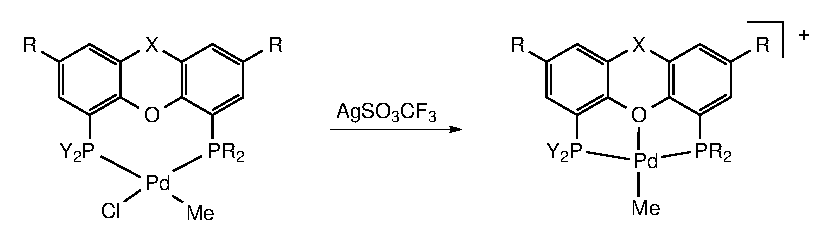
\includegraphics{../Schemes/Pdchloromethyl.eps}
\caption[Chloride abstraction from [PdClMe(xantphos){]}]{Chloride abstraction from [PdClMe(xantphos)] xantphos = \Phsixantphos{}, \Phthixantphos{}, \Phxantphos{}, and Me-xantphos.}
\label{Pdchloromethyl}
\end{scheme}

A variant of xantphos with ethyl substituents on the phosphorus atoms (Et-xantphos) was reported in 2004.\cite{Miedaner2004, Raebiger2004}  Palladium and platinum complexes, [M(Et-xantphos\ce{)2}], [M(Et-xantphos\ce{)2]^{2+}} and platinum complexes [Pt(Et-xantphos\ce{)2H]PF6} and [Pt(Et-xantphos\ce{)2(H)2]^{2+}} have been studied for their electrochemical properties.  The X-ray crystal structures of [M(Et-xantphos\ce{)2}] (M = Pd, Pt) were obtained and have a tetrahedral geometry, with average bite-angles of 108.3\degrees{} for both metals, while the palladium(II) complex had two molecules in the unit cell, one closer to a square-planar geometry (average bite-angle = 139.7\degrees) and the other closer to a tetrahedral geometry (average bite-angle = 95.8\degrees).  The pseudo-square planar [Pd(Et-xantphos\ce{)2]BF4} complex was also crystallised and had much larger bite-angles than any of the other ethyl substituted diphosphines that were part of the study (\gls{depp}, \gls{depx} and \gls{depPE}) indicating the ability of the xantphos ligands to support metals in an unusual geometries.  

A xantphos ligand with isopropyl substituents on the phosphorus atoms� \iPrxantphos{} was first reported in 2010, together with the osmium complex [Os(\iPrxantphosk)\ce{Cl3}], showing the \POP{} coordination which is common for xantphos ligands in octahedral complexes.\cite{Asensio2010}  The same group has since investigated the synthesis and reactivity of [M\ce{Cl2}(DMSO-\dento{}S)(\iPrxantphos)] (M = Os, Ru) producing a number of different osmium and ruthenium complexes including various polyhydrides and bis(alkynyl)vinylidene complexes.\cite{Alos2013, Alos2014}  

A study of the reactivity of \iPrxantphos{} towards palladium shows differences to the \Phxantphos{} ligand.\cite{Bakhmutov2012}  The [Pd(\ce{CF3})Ph(\Phxantphos)] complex exists in a \cis{} geometry in the solid state, and \cis{} and \trans{} isomers in solution, whereas the analogous \iPrxantphos{} complex shows only a \trans{} configuration.  The \iPrxantphos{} complex was synthesised in a different manner as the \Phxantphos{} ligand was readily displaced by \ce{CF3-} from \ce{CF3SiMe3}/\ce{F-} while the \iPrxantphos{} ligand was not, indicating the different chemistry of the two ligands.  The difference in the coordination geometries also meant the \ce{PhCF3} was more readily lost from the \cis-[Pd(\ce{CF3})Ph(\Phxantphos)] than the \trans-[Pd(\ce{CF3})Ph(\iPrxantphos)].  A related study investigated nickel complexes of \iPrxantphos{} for the trifluoromethylation of aryl halides.\cite{Jover2014}  The [NiF(1-naphthyl)(\iPrxantphos)] complex readily reacted with \ce{CF3SiMe3} to give [Ni(\ce{CF3})(1-naphthyl)(\iPrxantphos)].  Both of these complexes were found to have \trans{}-geometries through X-ray crystallography, and showed slow decomposition at 140 \degC{} and 120 \degC{}, giving rise to a range of products, with no C-F compounds or 1-trifluoromethylnaphthyl formed.  

The chemistry of rhodium and iridium complexes with \iPrxantphos{} have also been studied.  Reaction of \iPrxantphos{} with [Rh(\hapto{}-Cl)(COE\ce{)2]2} yielded the [RhCl(\iPrxantphosk)] complex cleanly.\cite{Esteruelas2013}  However, reaction with the iridium analogous resulted in cyclometallation of one of the isopropyl groups  forming [IrClH(\iPrxantphos-\dento{}-C,P,O,P\textprime].  The chloride ligand in [RhCl(\iPrxantphosk)], was replaced with a hydride, \emph{via} reaction with \ce{KO^{i}Pr}, producing KCl and acetone as by-products.  The trihydride [Ir(H\ce{)3}(\iPrxantphosk)] was produced by reaction of the metallated iridium complex with KOH, \ce{^{i}PrOH}.  The rhodium chloride complex readily splits hydrogen to form [RhCl(H\ce{)2}(\iPrxantphosk)].  The analogous iridium complex was synthesised by reaction of the metallated complex with \emph{n}-octane at 90 \degC.  Recent research has shown that the chloride can be removed from [RhCl(H\ce{)2}(\iPrxantphosk)] by reaction with \ce{Li[B(C6F5)4]OEt2} forming [Rh\ce(H\ce{)2}(\iPrxantphosk)].\cite{Haibach2013}  The [RhCl(\iPrxantphosk)] and [IrClH(\iPrxantphos-\dento{}-C,P,O,P\textprime] both form [MCl(H)(OTf)(\iPrxantphosk)] when reacted with triflic acid.\cite{Esteruelas2013}  The reactivity of the \iPrxantphos{} complexes is summarised in Figure \ref{RhiPrxantphos} and \ref{IriPrxantphos} for rhodium and iridium respectively.  

\begin{scheme}[htbp]
\centering
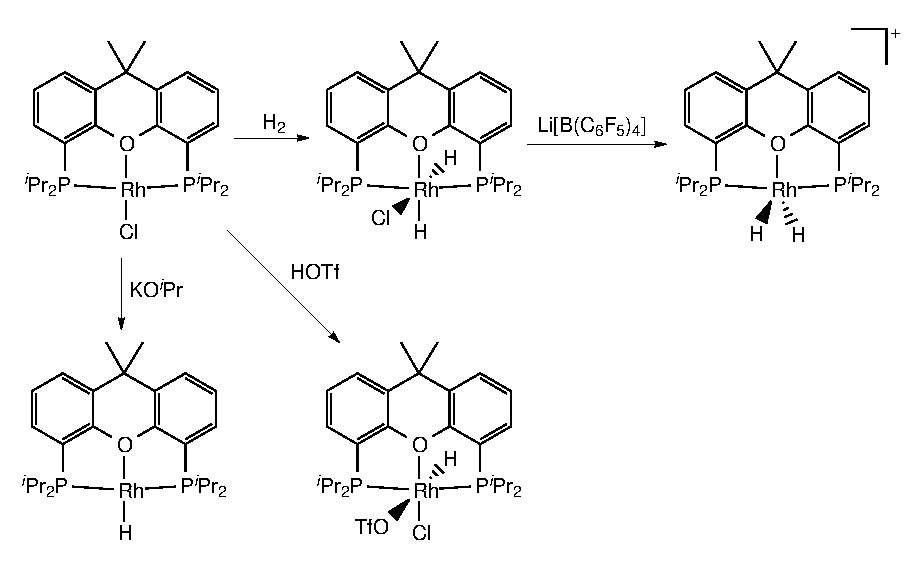
\includegraphics{../Schemes/RhiPrxantphos.eps}
\caption[Reactions of [Rh(\iPrxantphos){]}]{Reactions of [Rh(\iPrxantphos){]}.}
\label{RhiPrxantphos}
\end{scheme}

\begin{scheme}[htbp]
\centering
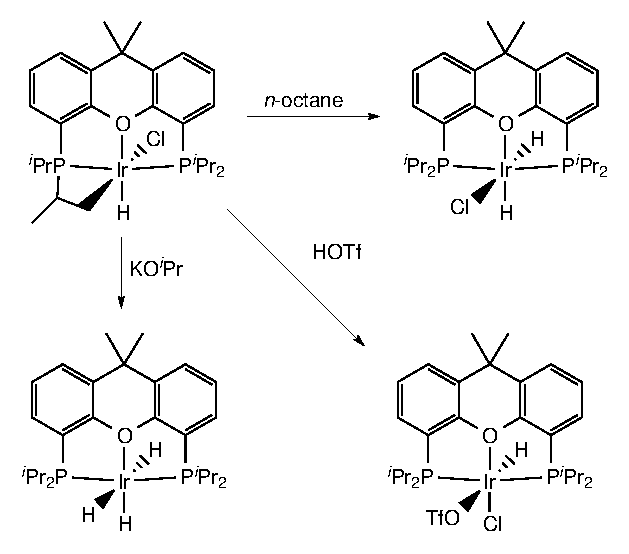
\includegraphics{../Schemes/IriPrxantphos.eps}
\caption[Reactions of [Ir(\iPrxantphos){]}]{Reactions of [Ir(\iPrxantphos){]}.}
\label{IriPrxantphos}
\end{scheme}

Further work investigated the reactivity of the rhodium and iridium complexes towards silyl compounds which are summarised in Figure \ref{IrRhsilyl}.\cite{Esteruelas2013b}  Reaction of [RhCl(\iPrxantphosk)] or [IrClH(\iPrxantphos-\dento{}-C,P,O,P\textprime] with \ce{SiH2Ph2} or \ce{SiHEt3} resulted in [MCl(H)(\iPrxantphosk)(Si\ce{R3}] (M = Rh, Ir. \ce{SiR3} = \ce{SiHPh2}, \ce{SiEt3}.  The diphenylsilane complexes are unstable in solution forming [Rh(Si\ce{ClPh2})(\iPrxantphosk)] \emph{via} loss of molecular hydrogen and \trans{}-[Ir(Si\ce{ClPh2)(H)2}(\iPrxantphosk)].  The rhodium complex [RhH(\iPrxantphos)] also underwent reaction with \ce{SiHEt3} and \ce{SiHPh3} initially forming the dihydride [Rh(H\ce{)2}(\iPrxantphosk)\ce{(SiR3)}] (R = Et, Ph) which loses molecular hydrogen to form [Rh(\iPrxantphosk)(Si\ce{R3})].  Reaction of [Rh(Si\ce{ClPh2})(\iPrxantphosk)] with \ce{NaBAr^{F}4} in the presence of water produced [Rh(H)(\iPrxantphosk)(\ce{SiOHPh2})] which was tested as a catalyst for the alcoholysis of \ce{H2SiPh2} with various alcohols in toluene at 32 \degC, forming ROSiH\ce{Ph2} in isolated yields of 71 - 92\% with \glspl{TOF} of 4000 to 76500 \si{\per\hour}.

\begin{scheme}[htbp]
\centering
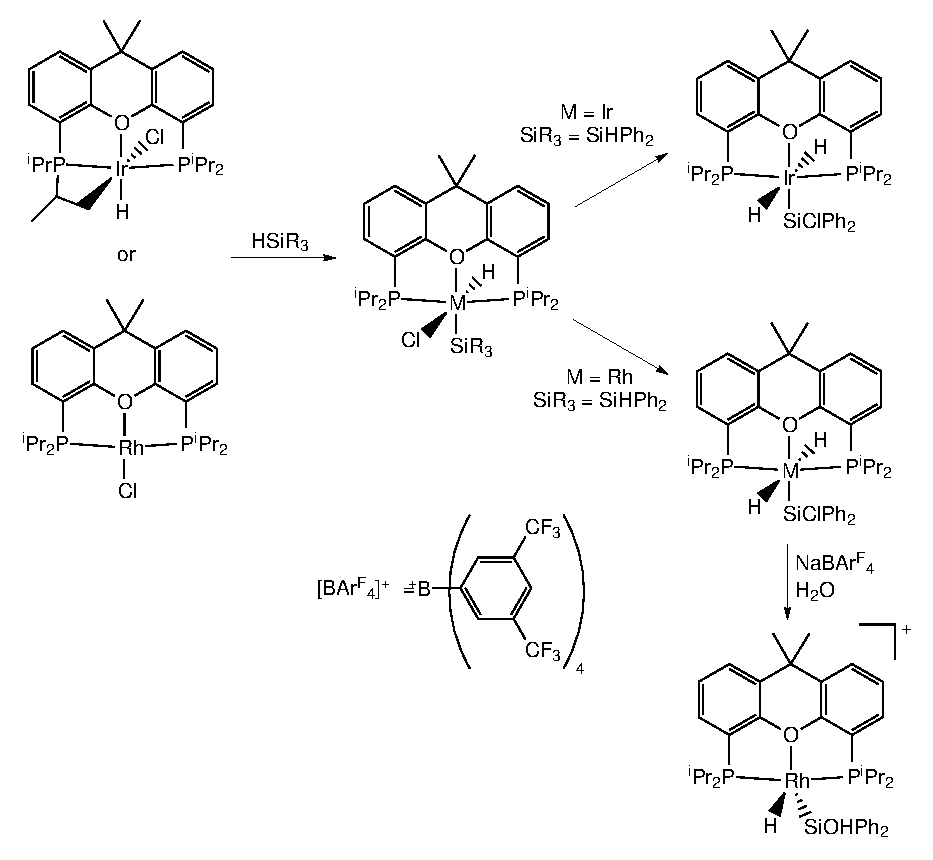
\includegraphics{../Schemes/RhIrsilyl.eps}
\caption[Reactions of Rh and Ir \iPrxantphos{} complexes with silanes]{Reactions of Rh and Ir \iPrxantphos{} complexes with silanes. \ce{SiR3} = \ce{SiHPh2}, \ce{SiEt3}}
\label{IrRhsilyl}
\end{scheme}

\subsection{\tBuXantphos}

This thesis covers an investigation into the coordination chemistry of three different xantphos ligands with \tBu{} substituents on the phosphorus atoms.  The three ligands differ in the bridgehead position from \tBuxantphos{} with \ce{CMe2}, \tBusixantphos{} with \ce{SiMe2} and \tButhixantphos{} with a thioether bridge.  The first mention of \tBuxantphos{} was in 2002 with the unsuccessful attempts to synthesise \tBuxantphos{} from either the dilithiated backbone or the 9,9-dimethyl-4,5-bis(dichlorophosphino)xanthene, citing steric crowding as the reason for the lack of reactivity.\cite{Zuideveld2002}  A successful synthesis of \tBuxantphos{} from the dilithiated backbone was reported in 2005 by heating the reaction mixture to 60\degC{} in order to proceed.\cite{Mispelaere2005}  \tBuXantphos{} has subsequently been studied for use as an ancillary ligand in the palladium catalysed cross-coupling of thiols and aryl bromides or triflates, the iron catalysed \ce{sp^3}-\ce{sp^3} cross-coupling of alkyl halides with alkyl Grignard reagents, the platinum catalysed amination of allylic alcohols and the N-arylation of heterocyclic diamines, all with poor yields, while higher yields were observed when \Phxantphos{} was used.\cite{Mispelaere2005, Dongol2007, Ohshima2009, Cabello2007}  All of these studies used catalysts formed in \emph{situ}, so the coordination chemistry was not investigated, although the reactivity suggests differences in the coordination chemistry of \Phxantphos{} and \tBuxantphos{}, warranting further investigation.

Prior to the start of this research, the only isolated coordination complexes of \tBuxantphos{} were [Au(\tBuxantphos)][\ce{AuX2}] (X = Cl, Br, I), formed by reaction of [AuCl(\acrshort{tht})] (\acrshort{tht} = \acrlong{tht}) with \tBuxantphos{} and subsequent reaction with KBr or KI.\cite{Partyka2010}  The analogous reaction using \Phxantphos{} gave the [(AuX\ce{)2}(\Phxantphos)] (X = Cl, Br, I) with each phosphorus atom coordinated to a separate gold centre with a Au-Au interaction.\cite{Pintado2004, Partyka2010}  Subsequent investigations into the catalytic activity of gold xantphos complexes towards the C-F bond activation of perfluoroarenes showed \glspl{TON} of 200 for [AuCl(\Phxantphos)] and 1000 for [Au(\tBuxantphos)][\ce{AuCl2}].\cite{Zhan2012}  Mechanistic studies into the reaction showed that [Au(xantphos)\ce{]+} was an important intermediate and is in equilibrium with the inactive [Au(xantphos\ce{)2}].  Due to the steric bulk of \tBuxantphos{} the equilibrium favours the two-coordinate species while for \Phxantphos{} the four-coordinate complex is preferred, resulting in lower activity.\cite{Zhan2012}  This clearly shows the difference between the two xantphos ligands and suggests that a difference in the coordination chemistry may be the reason for the lack of catalytic reactivity in the \tBuxantphos{} systems.  

Subsequent to the start of the research presented in this thesis \tBuxantphos{} has gained increasing attention, likely as a result of the ligand becoming commercially available.  In the six years 
from the first successful synthesis in 2005 to the start of this research in mid-2011, only the four papers discussed above were published investigating \tBuxantphos{}.\footnote{Two papers investigating the use of the dioxidised \tBuxantphos{} as a ligand on europium and samarium were also published in 2011 and 2012.\cite{Miyata2011, Miyata2012}}  However, the following three years showed increasing attention with 9 papers published\cite{Friis2014, Dang2013, Liu2013c, Raoufmoghaddam2013, Haibach2013, Ashcroft2013, Behr2013, Raoufmoghaddam2013b, Zhan2012} and 10 patent applications.\cite{Shang2010, Shang2011a, Shang2011b, Shang2011c, Shang2012a, Brandstadt2013a, Brandstadt2013b, Brandstadt2013c, Brandstadt2013d, Brandstadt2013e}

Further investigations into the catalytic properties of \tBuxantphos{} have been reported, without investigation into the coordination chemistry.  These include the  palladium-catalysed Suzuki cross-coupling of 2-(4-bromophenyl)-5-chloropyrazine with a benzimidazole boronic ester and hydroesterification of methyl oleate.\cite{Ashcroft2013, Behr2013} In both cases little conversion was observed when \tBuxantphos{} was used, though the \Phxantphos{} systems showed significant reactivity.  The aminocarbonylation of aryl bromides was performed with each of \Phxantphos{} and \tBuxantphos{} in an unusual mono-dentate coordination mode.\cite{Friis2014}  Little reactivity was observed with \tBuxantphos{}, while the \Phxantphos{} system gave the product in 92\% isolated yield.  In the rhodium catalysed reductive amination of aldehydes \tBuxantphos{} showed a 59\% total conversion with only 19\% selectivity for the desired product, while \Phxantphos{} had an 84\% conversion and 93\% selectivity.\cite{Raoufmoghaddam2013}   

In some cases the \tBuxantphos{} system is more active than the \Phxantphos{} system such as, the palladium catalysed N-alkylation of aniline with benzyl alcohol.\cite{Dang2013} the \tBuxantphos{} system showed near quantitative conversion at 100 \degC{} while the \Phxantphos{} system required 110 \degC{} showed only 63\% conversion.  Improved activity with \tBuxantphos{} compared to \Phxantphos{} was also observed in the palladium catalysed methylation of alkynyl C-H bonds with dimethyl sulfonium ylides.\cite{Liu2013c}  Under the same conditions a yield of 46\% was obtained with \tBuxantphos{} while only 15\% was produced using \Phxantphos{}.  \tBuXantphos{} and \Phxantphos{} can also have similar results, such as in the rhodium catalysed hydroamidomethylation of 1-pentene with acetamide, \Phxantphos{} and \tBuxantphos{} showed conversions of 83 and 80\% respectively with greater than 99\% linearity in both cases.\cite{Raoufmoghaddam2013b}  

Despite the increased interest in \tBuxantphos{} in the last four years, research has focussed on the catalytic behaviour of the transition metal complexes, mostly with the catalyst formed in \emph{situ}.  A crystal structure of \trans-[Pd(\tBuxantphos)\ce{Cl2}], was reported \emph{via} private communication to the \gls{CSD} in 2011 (CSD-XARXAR), no further publication of this complex has followed.\cite{Allen2002}  One paper has reported the coordination behaviour of the \tBuxantphos{} ligand with rhodium.\cite{Haibach2013}  Similarly to the work with \iPrxantphos{}, the \tBuxantphos{} ligand reacts with [Rh(\acrshort{coe})(\hapto{}-Cl)\ce{]2} (\acrshort{coe} = \acrlong{coe}) to give [Rh(\tBuxantphosk)Cl].  This Rh(I) chloride can readily split hydrogen to form a [Rh(\tBuxantphosk)Cl\ce{(H)2}] complex.  The structures of [Rh(\tBuxantphosk)Cl] and [Rh(\tBuxantphosk)Cl\ce{(H)2}] have been confirmed by X-ray crystallography.  Chloride abstraction from [Rh(\tBuxantphosk)Cl\ce{(H)2}] using \ce{AgBF4} or \ce{AgSbF6}, generates the trigonal bipyramidal dihydride complex Rh(\tBuxantphosk)\ce{(H)2}], with the \tBuxantphos{} ligand retaining the meridional coordination typical of pincer ligands.  This dihydride was found to react with ethene to give ethane and [Rh(\tBuxantphosk)(\ce{C2H4})], however no reaction with the commonly used hydrogen acceptors, \emph{t}-butylethylene or norbornene was observed, nor was any reaction with terminal alkenes.  [Rh(\tBuxantphosk)Cl\ce{(H)2}] reacts with \ce{KO^{t}Bu} resulting in a four-coordinate mono-hydride species [Rh(\tBuxantphos)H].  Addition of ethene to [Rh(\tBuxantphos)H] resulted in the reversible formation of an ethyl complex.  The [Rh(\tBuxantphos)H] also showed reactivity in the isomerisation of 1-hexene with a \gls{TON} of 2000 after 16 hours.  

The literature work on \tBuxantphos{} shows similarities and differences in the reactivity compared to \Phxantphos{}, particularly in catalytic applications. Although a number of palladium catalysed reactions have been studied, only two palladium complexes have been reported (one being only a crystal structure).  The only research into the coordination chemistry of the \tBuxantphos{} ligands is on gold and rhodium.\cite{Partyka2010, Haibach2013}  The original study into the xantphos ligands focussed on changing the bridging groups of \Phxantphos{} showing the impact that subtle changes in the bite-angle can have on the catalytic activity of the transition metal complexes.\cite{Kranenburg1995} Despite this, only one derivative of \tBuxantphos{} in the bridging position has been reported, with an isopropenyl substituent, and it has not been compared with \tBuxantphos.\cite{Marimuthu2012}  Given the number of studies investigating the catalytic activity of \tBuxantphos{} without investigating the coordination chemistry, an examination into the coordination chemistry of a range of subtly different \tBuxantphos{} ligands with late-transition metals is of particular interest.   

%===========================================================================
\section{Research Objectives}

The xantphos class of ligands have been the subject of a number of studies, with interesting and varied results.  The initial studies investigated the influence of changes in the bite-angle resulting from changing the group in the bridging positions from the \ce{CMe2} group found in \Phxantphos.\cite{Kranenburg1995, Kranenburg1998, Kamer2001}  These studies have shown a significant impact that small changes in the bite-angle can have on the catalytic reactivity and selectivity of the ligands.  Recently a large amount of research has focussed on the development of xantphos derivatives with alkyl substituents on the phosphorus atoms, particularly the \iPrxantphos{} and \tBuxantphos{}.  Prior to the start of this research only one study investigating the coordination behaviour of \tBuxantphos{} had been published.\cite{Partyka2010}  The other studies all showed much lower activity in catalytic systems than with the \Phxantphos{} ligand.\cite{Ohshima2009, Mispelaere2005, Dongol2007}   Together this suggested that the coordination behaviour of the \tBuxantphos{} and \Phxantphos{} ligands is different and deserved further attention.  The studies published since the inception of this research has only sought to solidify the objectives, as these have shown several examples of studies into the use of \tBuxantphos{} in catalytic systems with only one further study into the coordination behaviour on rhodium, despite the majority of the catalytic studies being performed on palladium.  Furthermore, despite the much larger bite-angle and electronic differences of \tBuxantphos{} compared to \Phxantphos, and the impact small bite-angle changes have on the activity of \Phxantphos{} only one derivative of \tBuxantphos{} in the bridging position has been published, and no comparative investigation has been published.

The over-arching goal of this research is to investigate the synthesis, properties and coordination chemistry of \tBuxantphos{} and two derivatives in the bridgehead position (S and \ce{SiMe2}).  The first stage will aim to synthesise the \tButhixantphos{} and \tBusixantphos{} ligands, and investigate the steric and electronic properties of all three \tBuxantphos{} ligands by the calculation of their natural bite-angles and synthesis of some non-transition metal derivatives.  

Silver is a particularly interesting metal for the synthesis of coordination complexes, showing a distinct propensity to form dimers, trimers, or higher order structures, and differences dependent upon the steric bulk and flexibility of the diphosphine ligands used.\cite{Meijboom2009}  Hence, the initial coordination chemistry of the three \tBuxantphos{} ligands towards silver will be investigated in order to gain an understanding of their coordination chemistry and gauge the impact of the steric bulk on their coordination chemistry, and to allow comparison to the gold \tBuxantphos{} complexes previously published.

The remainder of the research will focus on transition metals which are commonly used as homogeneous catalysts.  The xantphos class of ligands have been well-studied for their roles as ancillary ligands in hydroformylation.\cite{Veen1998, Veen1999b, Veen2002, Zuidema2008, Petocz2004, Bronger2003, Kranenburg1995}  The aim of this research is not to investigate the catalytic properties of the three \tBuxantphos{}, but to produce discrete transition metal complexes to gain insight into the catalytic studies that have already been performed.  Hence the coordination chemistry with rhodium will focus on the synthesis of a simple rhodium(I) complex and establish the reactivity towards small molecules, including hydrogen and carbon monoxide, which are the foundation for a number of different catalytic processes.  

The coordination chemistry of the three \tBuxantphos{} ligands towards palladium and platinum in both the 0 and +2 oxidation states will also be studied, in order to gain insight into the differences in the catalytic activity of systems with \tBuxantphos{} and \Phxantphos{}.  Palladium is one of the most widely used metals for homogeneous catalysis and catalytic cycles frequently involve interconversion between the two oxidation states.\cite{Tsuji1995}  Platinum complexes will be synthesised prior to the palladium investigation as the presence of an NMR active isotope (\Pt) coupled with the high stability of platinum complexes can be beneficial to the identification and characterisation of any complexes produced.  Although the coordination chemistry of \Phxantphos{} with palladium is well-known, few coordination complexes of \Phxantphos{}, and particularly \Phthixantphos{} and \Phsixantphos{} with platinum have been reported.  This work will begin with a brief investigation into the coordination chemistry of \Phthixantphos{} with platinum to assist in identifying any differences in the coordination chemistry that may result from changing the phenyl substituents to \tBu{} groups.  The coordination chemistry of the three \tBuxantphos{} ligands with palladium and platinum in the 0 and +2 oxidation states will then be performed.

Throughout this research \gls{NMR} spectroscopy will be used extensively to characterise the products of the reactions and aid in the identification of any intermediates or dynamic processes that may be present.  X-ray crystallography will also be an important tool, particularly to compare the bite-angles and coordination geometries of the \tBuxantphos{} complexes produced with those previously reported for the \Phxantphos.  \Gls{DFT} will also be used to gain further insight into reactions or processes when this is beneficial.


%\section{Tertiary Phosphine Ligands}
%
% They are very widely used in a range of catalytic transformations as ancillary ligands.  Bonding through the donation of the lone pair on the phosphorus atom, tertiary phosphines are considered strong sigma-donors and \fixme{pi}-acceptor ligands.  The strong bond that forms as a result of the donation from the phosphorus to the metal combined with back-donation from the metal centre \fixme{is there really back-donation?} allows tertiary phosphine ligands to bond very strongly to the metal.  This strong bond imparts a great deal of stability to the complexes allowing longer lifetimes in catalytic transformations, resulting in higher turnover numbers (TON, the maximum number of turnovers that a single molecule of catalyst can perform before degradation).  Similarly to other common ligands like N-heterocyclic carbenes (NHC) the tertiary phosphine ligands impart a great deal of control over the metal centre.
%
%The tertiary phosphine ligands can be derivatised in a number of different ways to change the properties of the phosphine.  Unlike NHC ligands which typically have an imidazolium core, which means that derivatisation occurs further away from the coordinating atom, tertiary phosphines can be derivatised directly in the alpha position meaning that changes have a much greater impact on the metal centre, thus affecting its reactivity and selectivity in a range of different ways, hence having a great impact on the different catalytic processes that a metal may undertake.
%
%Tertiary phosphines are typically used in catalytic transformations as ancillary ligands.  Ancillary ligands are ligands that are not directly involved in the catalytic process (though they may \fixme{de-ligate} and then re-coordinate to allow for free coordination sites for the catalytic reagents).  However, ancillary ligands can impart a great deal of control over the reaction taking place.  Changing the ligand to a different ligand may result in different regio- or stereoselectivity, or it may change the nature of the product entirely (polyketone rather than methyl methacrylate for dbpx reaction).  Furthermore changing the ligand may have a dramatic effect on the nature of the product and the rate of reaction.  As previously discussed the phosphine imparts a great deal of stability to the metal centre meaning higher turnover numbers.  Catalysis is a fine balance between meeting the stability requirements so the catalyst undergoes a large number of turnovers before degrading and ensuring that there is enough instability in the system so that it isn't a rock and actually loses some ligands to form free coordination sites for the catalyst to coordinate to and that the resulting "resting state" is unstable enough so that it progresses through the catalytic cycle.  
%
%Altering the groups coordinated to the phosphorus can also change the steric and electronic environment around the metal centre.  A number of asymmetric ligands such as BINAP and CAMP are chiral ligands used in asymmetric catalysis such as the synthesis of L-dopa an important drug used in the treatment of Parkinson's disease.  These ligands are able to control the steric environment around the metal centre such that the substrate will prefer to coordinate to a particular site or in a specific geometry thus allowing chirality to be introduced in the product.  This is one important application for asymmetric catalysis.  However, there are a number of different ways in which the steric bulk of a system may impact the catalytic transformation.  For example, a non-chiral but sterically bulky ligand may result in coordination of different combination of substrates by selectively allowing coordination at the terminal of a molecule rather than in the middle of a chain.  For polymerisation of ethene this may result in linear chains, thus forming high density polyethylene rather than the branched low density products.  For other reactions sterically bulky ligands may enhance certain geometries of transformations.  For example an alkyl migration may occur more favourably to form a linear rather than branched product.  This is important for a number of reactions such as hydroformylation or other carbon-carbon reactions involving alkenes such as hydroesterification, allylic alkylation or alkoxycarbonylation.  Using sterically bulky phosphines as ancillary ligands can also prevent side-reactions occurring leading to large distributions in the products.
%
%Large sterically bulky ligands can also promote a number of different steps that occur in catalytic transformations.  Frequently the rate-determining-step involves the coupling of two ligands in a reductive elimination.  As such, the presence of large ligands which restrict the space around the metal centre can enhance the speed with which this occurs generally by destabilising the starting intermediate \fixme{the thing before it has reductively eliminated}.  The sterically bulky ligands can also reduce the degradation pathways by preventing the formation of inactive materials such as by having two of the same substrate coordinate to the metal.  They can also reduce the likelihood of degradation from molecules such as oxygen or nitrogen coordinating to the metal centre.  
%
%\subsection{Electronic and Steric Parameters}
%
%Attempts have been made to quantify the steric and electronic nature of tertiary phosphine ligands.  
%In order to analyse and compare the electronic properties of tertiary phosphine ligands an indirect measure of their donor ability is required.  %
%\section{Diphosphine Ligands}
%
%Diphosphine ligands are ligands that consist of two tertiary phosphine groups linked by some sort of backbone.  Most typically this takes the form of a carbon skeleton such as an ethyl, propyl or xylyl group as found in 1,2-\emph{bis}-diphenylphosphinoethane (dppe), 1,2-\emph{bis}-diphenylphosphinopropane (dppp) or dbpx \fixme{what is dbpx's full name?}.  Some more unusual backbones include the pyridyl backbone found in a number of pincer ligands, and a ferrocene molecule such as that found in diphenylphosphinoferrocene (dppf).  Diphosphines are particularly interesting molecules as having two phosphorus donor ligands joined through a backbone allows further control over the geometry of the coordination complex.  This additional control can be displayed through changes in the reactivity, selectivity and regioselectivity of various different catalytic transformations.  Diphosphines are able to exert more control over the metal centre and as such they can have dramatic changes to the reactivity compared to a catalyst comprised of two monophosphine analogues.  
%
%The additional stability of diphosphine complexes is a result of the chelate effect.  During catalysis it is quite common for the metal complex to lose ligands in order to form free coordination sites in order for the substrates to coordinate and thus allow the catalytic transformation to take place.  For monophosphine ancillary ligands frequently the ligand is lost and then needs to compete for the free coordination site with the substrates once the reaction is complete.  This can lead to significant degradation of the catalyst and is generally overcome by addition of some free phosphine ligand.  However, the phosphine is still generally not the major component of the reaction mixture as doing so may result in complexes that are coordinatively saturated with the phosphine ligand and henceforth display reduced reactivity.  For a diphosphine ligand, if one arm of the ligand has dissociated in order to make room for the substrate molecules, the diphosphine ligand is still connected to the metal centre through the other arm of the diphosphine.  This holds the uncoordinated arm in close proximity to the metal centre and thus increases the effective concentration of the ligand from the perspective of the metal.  This chelate effect is an entropic effect which supposes the intramolecular reactions are always preferred over intermolecular reactions as intermolecular reactions have a decrease in the overall entropy of the transformation (i.e. two molecules continue as two individual molecules rather than the two molecules reacting to form a single entity).  Overall this has the effect of maintaining the disorder (number of molecules) in the system rather than decreasing it as would happen if another substrate coordinated rather than the other arm coming back in.
%
%In square planar and octahedral complexes diphosphine ligands typically occupy a \cis{} geometry while the analogous monophosphines frequently have a thermodynamic driving force to form the \trans{} isomer.  This locking-in of a \cis{} geometry means that the catalyst should remain in a \cis{} form throughout a catalytic process.  This means that a common degradation pathway - namely the isomerisation to a \trans{} complex - is avoided through the use of a chelating disphosphine.  This can enhance the turnover numbers and even the turnover frequency as isomerisation is not a possibility.  Numerous catalytic process exist where changing from monophosphines to a diphosphine has altered not only the reactivity by also the selectivity of a reaction.  In addition having a chelating ligand imparts further stability on a complex without affecting it's reactivity \fixme{lies?} this means that the diphosphine complex may be able to undergo more turnovers before degrading, thus resulting in a higher yield from the catalytic reaction.  In addition one of the phosphorus atoms may be able to \fixme{de-ligate} and form a free coordination site enabling the catalytic cycle to progress while still imparting the stability that comes from having a phosphine ligand.  In addition once the reaction has progressed and the coordination site is no longer needed the phosphine is held in close proximity to the metal such that this arm of the diphosphine is more likely to recoordinate and reform the catalyst resting state rather than another molecule of substrate coordinating and potentially leading to catalyst degradation.  
%
%Trigonal bipyramidal structures are very common intermediates for catalytic transformations, especially those involving rhodium like hydroformylation.  In these complexes diphosphine ligands can typically coordinate in two different geometeries.  Namely a \emph{bis}-equatorial complex or an axial-equatorial mode.  There is a further possibility of a \emph{bis}-axial mode.  However, this is unlikely as the equatorial ligands will impose steric restrictions on the diphosphine ligand preventing it from forming a \emph{bis}-axial complex.  It is quite common to switch between octahedral, trigonal bipyramidal, square-planar or tetrahedral complexes in a catalytic cycles.  Each of these can form a number of different isomers.  If a ligand is able to exert steric or electronic restrictions on the metal geometry that can form then some of these will be more or less favoured from a thermodynamic or kinetic perspective.  This means that the diphosphine ligand can control the geometry of the intermediates and thus control the manner in which the reactions proceeds, thereby control the product distribution and potentially altering the regioselectivity and stereoselectivity of a system.  This may also have a significant impact on both the turnover number (if the diphosphine can promote stable complexes) and the turnover frequency. 
%
%In a similar manner to monophosphine ligands, diphosphine ligands can be described using the electronic parameters described earlier.  However, in there are a few minor differences.  Namely, as discussed previously, diphosphine ligands typically coordinate in a \cis{} geometry, this means that the series are not directly comparable as there will be an effect from the different geometries.  This is most prominent in the rhodium series of \ce{[Rh(CO)ClL2]} complexes as one of the phosphorus atoms will be \trans{} to a carbonyl while the other will be \trans{} to a chloride ligand.  The parameters determined by NMR spectroscopy will be most affected by this as the \trans{} influence has a large effect on the coupling constants.  In the \ce{[PtCl2(monophosphine)2]} and the \ce{[Rh(CO)Cl(monophosphine)2]} complexes the electronic properties of the ligands were able to be determined as the ligand was \trans{} to an identical phosphine.  However, when using a diphosphine the most likely geometry is a \cis{} configuration.  Hence in the platinum dichloride complexes the phosphorus atoms of the diphosphine ligand will be \trans{} to chloride ions which typically have a relatively low \trans{} influence and is typically lower than a phosphine.  As such the value for the platinum phosphorus coupling constant will be larger than those reported for the \trans{} monophosphine complexes.  In the rhodium complexes, given a \cis{} geometry, one of the phosphorus atom will be \trans{} to a carbonyl ligand and the other phosphorus atom will be \trans{} to a chloride ligand.  A carbonyl ligand has a much higher \trans{} influence than a chloride ligand. \fixme{what is a CO's trans influence?}  This means that the rhodium phosphorus coupling constant for the phosphorus \trans{} to the chloride will likely be higher than that reported for the monophosphine complexes, while the phosphorus rhodium coupling constant for the phosphorus \trans{} to the carbonyl will likely be lower than that for the monophosphine analogue.
%
%The cone angle parameter can be determined for diphosphine ligands.  However, like the electronic parameter it is not directly comparable with those determined for monophosphines.   \fixme{but Tolman compares them directly in his 1977 paper c.f. appendix B}  For diphosphine ligands Tolman describes a method of determining the cone angle which is slightly different to that for monophosphines.  In this case $\theta/2$ can be described by the angle between one M-P bond and the bisector of the PMP angle (the bite-angle) \fixme{this is kinda confusing}.  This allows for direct comparison between the monophosphines and their diphosphine analogues.  For example the cone angles of dppm, is 121\degrees{} and dppe is 125\degrees{} whilst the cone angle of their monophosphine analogues are 136\degrees{} for both \ce{PMePh2} and \ce{PEtPh2}.  From this we can see that the cone angle of diphosphines is typically smaller than that for the monophosphine analogue.  This may be an effect of the relatively short backbone lengths for these two ligands which means that the backbone pulls it back together this reducing the cone angle.  
%
%While the cone-angle is a valid measure of the steric impact of a given monophosphine or diphosphine ligand it does not give the best indication of the steric influence of a diphosphine on the other ligands in the complex or for predicting the preferred coordination geometry of a given diphosphine ligand.  One of the more commonly utilised parameters for diphosphine ligands in the bite-angle.  This is the P-M-P angle for a given complex, it can be determined in two ways.  The first is a computational method whereby the ligand geometry is optimised for a chelating rhodium complex with no other ligands and the  rhodium atom situated at 2.315 \si{\angstrom} from each of the phosphorus atoms.  This method gives typically uses molecular mechanics parameters to optimise the structure.  Using this method enables the determination of the natural bite-angle i.e. the bite-angle determined using only the ligand parameters and is sometimes referred to as the ligand-preferred bite-angle.  The natural bite-angle is also useful as a way of predicting the ligand properties before the ligand is synthesised so it can be used to identifying the candidates for a particular reaction without needed to actually synthesise the complexes.  The natural bite-angle is general calculated in conjunction with a flexibility range.  This is the range of angles that the ligand can obtain within 2 kcal\si{\per\mol}.  This also allows for some indication of the rigidity of a ligand which can be useful for predicting the coordination chemistry.  
%
%The bite-angle can also be determined crystallographically.  This is useful to have an experimentally determined value.  However, the bite-angle a diphosphine ligand will display in a given context is highly dependent on the natural of the metal, the preferred geometry for that metal in a given oxidation state.  It is also dependent on the other ligands that are present such that sterically bulky ligands in a position \cis{} to one of the phosphorus atoms of a diphosphine ligand will result in a larger bite-angle than in an analogous complex with much smaller ligands.  Furthermore the \trans{} influence of the ligands that are \trans{} to the diphosphine will affect the bite-angle regardless of their steric nature.  If a phosphorus atom is \trans{} to a ligand with a strong \trans{} influence the phosphorus metal bond length will be longer than if it was \trans{} to a ligand with a weak \trans{} influence.  Although small the changes in the phosphorus metal bond length will have a dramatic impact on the determined value of the bite-angle.  In essence, while crystallographically determined bite-angles are interesting and useful for comparisons for a given ligand (i.e. how does the bite-angle change in \ce{[PtCl2(diphosphine)]} compared to \ce{[PdCl2(diphosphine)]}), in order to compare the bite-angles for two different ligands it is necessary to have crystal structures of analogous complexes.  However, in the solid state it is also possible for the crystal packing to impact the bite-angle by forcing the complex to adopt a rigid configuration.  Henceforth the natural bite-angle is the preferred way of comparing many different diphosphine ligands (and indeed bidentate chelating ligands in general) without needed to not only synthesise complexes for comparison but also grow X-ray quality crystals and obtain the single-crystal X-ray structure.
%
%The impact that changing the bite-angle of a chelating diphosphine ligand can have on the coordination behaviour of a complex is dramatic.  The bite-angle can effect the sites that the diphosphine ligand will preferential coordinate in.  A ligand like dppm with a natural bite-angle of 73\degrees{} will preferentially coordinate in sites that are idealised as 90\degrees{}, for example, \cis{} in square planar complexes and in an axial-equatorial mode in trigonal bipyramidal structures.  However, ligands with a larger bite-angle like BISBI with a natural bite-angle of 123\degrees{} is more likely to coordinate in a \emph{bis}-equatorial mode and this is closer to the preferred bite-angle.  The bite-angle of the diphosphine ligand can also stabilise some intermediates over others.  So dppm will likely stabilise complexes that are square-planar rather than those that are tetrahedral, while larger bite-angle ligands may promote the formation of tetrahedral of trigonal bipyramidal structures.  Furthermore the bite-angle of a diphosphine ligand can have a significant impact on the speed of some reactions by destabilising especially stable intermediates.  For example ligands with larger bite-angles are likely to promote reductive elimination reactions to increase their share of the space around the metal centre, likewise these ligands may promote migration reactions which also increase the amount of space that they can occupy.  Conversely the ligands with small bite-angles can promote oxidative addition of substrates as they have little steric barrier to the reaction occurring thus resulting in an electronic driving force, generally for the ligand to increase the number of electrons that it has, in order to get closer to the ideal 18.  In addition the bite-angle can have an impact on the regioselectivity and stereoselectivity of a reaction.  Similarly to the impact of changing the steric bulk of monophosphine ligands, although the bite-angle is not only a steric effect, increasing the bite-angle does increase the steric influence of the diphosphine ligand on the other ligands in the complex.  This means that although a reaction may typically give a branched product with a small bite-angle diphosphine ligand, changing to a large bite-angle diphosphine may result in a linear chain forming instead.  In addition changing the bite-angle may have an impact on the product distribution.  If using a chiral ligand a larger bite-angle may impart more stereoselectivity as the larger diphosphine ligand will impose more steric demands on the ancillary ligands thus making a particularly coordination geometry or rotamer to be favoured significantly over other resulting in an increasing enantiomeric excess.  
%
%As previously discussed monophosphine ligands frequently coordinate in a \trans{} configuration when under thermodynamic control regardless of the geometry of the starting complex.  Indeed \cis{} to \trans{} isomerism is very common in coordination chemistry.  Some \cis{} complexes are known, such as the well-known complex \ce{[PtCl2(NH3)2]}, cisplatin.  This complex is used widely as a chemotherapeutic agent from the treatment of a number of different cancers including childhood leukaemia.  Platinum is not a particularly labile metal centre, particularly platinum(II) however, the synthesis of cisplatin still requires careful control to avoid isomerism.  Further research into different the use of platinum compounds for chemotherapy has resulted in newer generations of platinum chemotherapeutic agents many of which use bidentate chelating ligands to force a \cis{} geometry as this is important for the mode of action of the drug (coordinates to DNA requiring two \cis{} coordination sites).
%
%\section{Xantphos}
%
%The xantphos class of diphosphine ligands have been widely studied with numerous reviews published about their coordination behaviour and the use of complexes formed with them as ancillary ligands have been tested in a huge number of different catalytic transformations.  The ligands were first reported in 1995 by van Leeuwen et al.\cite{Kranenburg1995}.  The xantphos class of ligands were the first ligands where the bite-angle effect was studied in a systematic manner.  The xantphos ligands consists of a rigid tricyclic backbone structure with two aryl rings bridged by an oxygen (in the site closest to the metal) and another bridging groups furthest from the metal centre.  By changing this group from a dimethylsilyl (\Phsixantphos) to a sulfur (\Phthixantphos) or a dimethylmethylene (\Phxantphos) or a simple bond between the two aryl rings (DBFphos) the researchers were able to make small changes to the bite-angle and study the effect that this had on the rhodium catalysed hydroformylation of 1-octene and styrene.  The ligands were found to have bite-angles (flexibility range) of 108.7 (93-132), 109.4 (94-130), 111.7 (97-135) and 131.1 (117-147) for \Phsixantphos, \Phthixantphos, \Phxantphos and DBFphos respectively.  
%
%From a nomenclature perspective xantphos is used in the literature to mean either the general class of ligands or the specific ligand.  In this thesis we will use the term \Phxantphos{} to describe the specific ligand and xantphos to describe any ligand of the class with derivatisation at any point.  Although efforts will be made to refer to the specific ligands it is useful to have a term to describe the class as a whole.  Similarly as we will be dealing with derivatives with \tBu{} groups as substituents on the phosphorus atoms, it is useful to refer to the group of the \tBu{} derived ligands without referring to the specific ligand \tBuxantphos{}.  We will endeavour to make it clear from the context and the use of figures and  compound numbering which specific case we are describing.  In order to discuss the xantphos ligands in more depth and refer to specific sites in the ligands we will talk about the bridgehead group, the backbone position and the phosphorus substituents.  These are the relevant positions when describing xantphos.  Using \Phthixantphos{} as an example the bridgehead position is occupied by a sulfur atom.  The methyl groups are in the backbone positions and the phosphorus substituents are phenyl rings.  From time to time we also may refer to a ligand by which group is in the bridgehead position.  Hence \Phthixantphos{} could be described as sulfur bridged, \Phsixantphos{} as silicon bridged and \Phxantphos{} as carbon bridged.  
%
%Since their initial inception in 1995, numerous publications have reported derivatives of the xantphos ligands.  Beyond the initial \Phsixantphos, \Phthixantphos{} and \Phxantphos ligands numerous different derivatives have been reported (although related DBFphos and DPEphos are not generally considered part of the xantphos class of ligands).  There are numerous sites for derivatisation of the xantphos ligands.  Changing the bridging group in the backbone - as was done in the original paper - has continued with tertiary amines and phosphines, di-\tBu-methylene, and alkenes to mention just a few.  Changing to a pnictogen also allows for a single groups or chain to be present at the bridgehead which can itself be further derivatised.  Other derivatives have changing the bite-angle by adding a benzene ring fused with the bridgehead carbon and one C-C bone of the aryl system.  Further derivatives have simply changed the length of the bridge by replacing the dimethylmethylene group with an ethyl linker.  Other derivatives of xantphos have changed the groups on the aryl system where the thixantphos methyl groups are located.  These have been changed to \tBu{} groups or to sulfate groups to impart either steric bulk (and change the electronics by adding the electron donating groups) or water solubility.  
%
%However as with most classes of diphosphine ligand the most common and potentially most interesting derivatives are those with different substituents on the phosphorus atoms.  In the case of xantphos a huge array of different substituents have been reported.  These include simply derivatising the phenyl rings of xantphos to change the electronics and impart more steric bulk, or changing to a different group entirely.  The relatively simple substitutions of the phenyl rings with isopropyl or \tBu{} groups have only been reported relatively recently.  Although methyl and ethyl substituents have been reported earlier.  Of course it is possible to replace only one of the phenyl rings such at with the MePh-xantphos ligand which has one methyl and one phenyl ring on each phosphorus atom.  In general derivatives of the xantphos class have involved the highly elaborate.  There has been a lot of research done with the derivatives which look like they have an entire xantphos skeleton on each phosphorus.  There are a number of different cyclic systems that make up other derivatives.  The xantphos ligands have also been derivatised with a specific purpose in mind, for example the previously mentioned sulfoxantphos which has sulfate groups in the backbone position and another xantphos derivatised with pendent amine groups on the phenyl rings on the phosphorus both of which impart water-solubility and have been studied for their use in biphasic catalytic systems.  In addition the recent drive towards asymmetric catalysts (as noted by the 2001 noble prize awarded to Knowles, Noyori and Sharpless) together with their high level of regioselectivity found in xantphos ligands has led to the synthesis of chiral xantphos derivatives such as (R,R)-Duxantphos and (R,R)-Duthixantphos.  
%
%All of these ligands obviously have different bite-angles.  The rigid backbone of the xantphos class of ligands imparts a starting level which is a rather large bite-angle.  As such the two ligands of the xantphos class with the smallest natural bite-angles are homoxantphos (102\degrees{}) and DPEphos (104\degrees).  Homoxantphos is the xantphos ligand with the ethane bridge rather than a single atom bridge.  This ethane bridge means that the aryl rings are further apart which in turn forces the phosphorus atoms closer together, thus resulting in the small bite-angle.  DPEphos is not technically a xantphos ligand as it is missing any atom in the bridgehead position which leads to dramatic twisting not available to the other xantphos derivatives.  Most of the xantphos derivatives occur with natural bite-angles of between 108\degrees{} and 124\degrees.  This large bite-angle leads to favouring of the tetrahedral and \emph{bis}-equatorial coordination modes, though as will be discussed soon, several different bonding modes are available to the xantphos ligand class.  The largest natural bite-angle for a xantphos ligand is for \tBuxantphos{}.  In this case the phosphorus substituents have been replaced with \tBu{} groups.  It is worth noting at this point that in the literature the term \tBuxantphos{} is used for the derivative with \tBu{} groups on the phosphorus atoms and also for the derivative with \tBu{} groups in the backbone position and phenyl substituents on the phosphorus atom.  For the purposes of this thesis it will become important to distinguish between them so \tBuxantphos{} will be used to described the specific ligand with \tBu{} groups on the phosphorus atoms (and the class of ligands with different bridgehead groups but still \tBu{} groups on the phosphorus atoms).  In situations where it is necessary to refer to the ligand with \tBu{} groups on the backbone positions we will use \tBu-\Phxantphos instead, consistent with our previous naming convention of the \Phxantphos{} ligands.
%
%At this state, although the xantphos ligands were first investigated to determine the impact of slight changes in the bite-angle in the product distribution of rhodium catalysed hydroformylation of 1-octene and styrene no study since then has looked at the bite-angle effect systematically for these other derivatives.  A lot of the derivatives mentioned have involved replacing the electron withdrawing phenyl substituents with electron donating alkyl groups, thus having a dramatic effect on the electronics of the system.  However, once the substitution has been made at phosphorus the researchers then compare directly using only the bite-angle as a means for comparison although changing the electronic may also be significant.  While the bite-angle encompassed both electronic and steric components it is primarily considered a steric effect.\fixme{is this really actually correct?}  Therefore in the literature there is a lack of research into the impact of small changes in the bite-angle on the coordination chemistry and catalytic activity of the larger bite-angle ligands.  Furthermore while the xantphos ligands have been investigated for catalysis, the differences in coordination chemistry the may occur as a result of small changes in the bite-angle have not been addressed.  As the \tBuxantphos{} ligand has a significantly larger bite-angle than the other ligands, combining with the electron donation of the \tBu{} substituents, thus resulting in a very electron rich phosphorus atom, the coordination behaviour may be quite different to that described for \Phxantphos{} and small changes in the bite-angle may result in large changes in the coordination chemistry.  
%
%Although the xantphos ligands were first investigated as diphosphine ligands for use in catalytic hydroformylation and have been widely studied as ancillary ligands in a large number of different catalytic processes, and as such their coordination chemistry has been described with relation to the catalytic processes.  Hence, the impact of small changes in the bite-angle on the coordination chemistry has not been studied in sufficient depth and has certainly not been studied with the very large bite-angle \tBuxantphos{} ligands.
%
%The xantphos class of ligands have a huge array of different bonding modes available.  Although the rigid backbone imparts the system with a relatively small array of available angles the system can twist and buckle in order to achieve much smaller backbones than the bite-angle might otherwise imply.  Xantphos is able to act similarly to most diphosphine ligands and form \cis{} complexes with square-planar geometries such as those found in palladium(II) which has been investigated with xantphos for cross-coupling catalytic transformations.  However, unlike most diphosphines it has also been reported that xantphos can act as a \trans-spanning diphosphine ligand and coordinate to square planar complexes in a \trans{} bidentate chelate geometry.  This is very unusual and will be discussed further in a bit.  Xantphos typically shows a preference for \emph{bis}-equatorial coordination which means that this can be used to control the regioselectivity and product distributions in various catalytic systems such as those based around rhodium.  Xantphos also shows a clear preference for tetrahedral coordination. Which makes sense, given that the bite-angle of 108\degrees{} is so close to the ideal bite-angle in a tetrahedral complex.  Although unusual, with some metals such as gold, xantphos can act as a monodentate phosphorus ligand.  This is highly unusual as the xantphos system is highly pre-arranged to prefer chelation.  Furthermore the xantphos ligand has also been known to act as a bridging bidentate ligand.  This is again quite uncommon and unusual as xantphos is pre-arranged to enhance chelation.  For \Phxantphos{} a search of the CCDC will yield diphosphine coordination complexes with bite-angles ranging from 98.8 to 153.1\degrees{} with an average of 108.5\degrees(from 65 structures).  This indicates that whether in a \cis{} of \trans{} geometry the ligand is strained and is only able to achieve the idealised angles of a square planar or octahedral complex.
%
%Trans-spanning diphosphines are highly unusual ligands.  The complexes of \Phxantphos{} that exist in a \trans{} geometry have only been isolated as a mixture of \cis{} and \trans{}.  This indicates that the strain that occurs to force the ligand into a \trans{} configuration is somewhat comparable to that required to force a \cis{} conformation.  However, as previously discussed the largest crystallographically determined bite-angle for the \Phxantphos{} ligand is 153.1\degrees{}.  Although this is much larger than the natural bite-angle reported for \Phxantphos{} it is still almost 30\degrees{} smaller than in an idealised square-planar complex indicating significant distortion of the coordination planar in order to achieve the \trans{}-chelation.  Diphosphine ligands that exhibit exclusive \trans{} coordination have been described in a review as elusive as most distort the coordination plane significantly or are able to be forced into a \cis{} geometry under the right circumstances with sufficiently bulky ancillary ligands.  Given their scarcity, the development of additional \trans{} spanning ligands together with further coordination complexes will contribute to the knowledge base of these unusual structures and potentially lead to novel catalytic processes.  
%
%Xantphos has been typically and widely referred to as a diphosphine ligands, however there is an oxygen present in the bridge which is relatively close to the metal centre.  This oxygen has the potential to coordinate to the metal centre and form a pincer-type complex (pincer ligands will be discussed in more detail further).  Complexes of this type are known for \Phxantphos{} however, the bidentate coordination is much more common.  The coordination of the oxygen to the metal centre imparts an added stability to the system and relieves the strain of the large bite-angles required for \trans{} chelation of the phosphorus atoms.  This forms a tridentate chelating ligand which has a high level of rigidity and can thus control the steric environment around the ligand imparting a great deal of control over the less controlled ligands.  This coordination can also impart a high level a rigidity on the system and thus result in the system being less susceptible to attack and degradation by other molecules including oxidation etc.  The rigidity can also lead to increased thermal stability.  This is important for homogeneous catalysis.  A number of catalytic systems require heating and generally they are faster at higher temperature.  However, the high temperatures can result in degradation of the catalyst especially to form nano particles (hot injection of a transition metal complex is in fact a very common method to synthesising nano particles).  These nano particles can be are in fact a heterogeneous catalyst for the same reaction, however, as the diphosphine ligand is no longer coordinated the impactt of the careful steric and electronic properties of the ligand in order to control the reaction are no longer of any effect.  Hence the catalytic reactions are frequently conducted at lower temperatures.  These lower temperatures mean that the rates are slower which can also mean lower yields.  Essentially it is a careful balancing act.  Using a complex with a xantphos ligand in a tridentate coordinate mode can impart added stability which means that the complex is less likely to fall apart at high temperatures, thus meaning that you can run the catalytic reaction at high temperatures without forming nano particles.  This means that you get all of the added benefits of homogeneous catalysis such as the additional regioselectivity and stereoselectivity from a carefully designed ligand system and your catalyst is in the same phase as the substrates meaning higher rates of reactivity as you are dealing with single molecules as catalysts rather than nano particles where reaction can only occur at the surface.  
%
%However, the majority of catalytic processes require multiple coordination sites for the substrates.  As previously discussed for diphosphine versus monophosphines it is possible for one arm to dissociate to form a free coordination site.  However, this means that that arm of the diphosphine ligand is unable to influence the reaction as it proceeds.  Ideally we would like part of the system with little impact on the coordination behaviour and geometries of the other ligands to dissociate so that the diphosphine can still impact the coordination behaviour and general catalytic process.  This is why xantphos is awesome.   The ether bridge bonds only weakly to the metal centre of the late-transition metals of the second and third.  In fact it is unlikely that it will coordinate to the metals at all, when they are in low oxidation states.  This means that the ligand can display hemilability, whereby the ether bridge can dissociate thus forming a free coordination site for a substrate molecule.  However, because the two phosphine atoms are still coordinated the benefits of having a diphosphine ligand and all of the careful ligand design and planning are not lost when the oxygen dissociates.  Once the reaction is complete and the product dissociates from the metal centre, the oxygen atom can recoordinate thus imparting the desired stability.  Due to the planar nature of xantphos the oxygen is in the centre of the molecule rather than one pendent arm. This means that the oxygen does not change the steric environment around the metal by coordinating or dissociating.  This can be desirable when performing catalytic reactions where the steric control imparted by the ligand is drastically important for the outcome of the reaction, such as in hydroformylation where branched and linear products can be produced depending on the outcome of the migratory insertion step.  In this case the linear product is the one that is most highly desired meaning that it is of far more value to the industry than the branched product and in the interests of atom efficiency and green chemistry it is desirable to only produce the product that is of actual use.  Rather than just pouring it down the drain or sticking it in a landfill somewhere, or burning it and producing greenhouse gases.  
%
%In addition for some catalytic processes carried out on palladium which generally only coordinates to four ligands, using a tridentate ligand can mean that the typically palladium zero/palladium(II) catalytic cycle is not accessible.  This meaning that for some systems a palladium(II)/palladium(IV) catalytic cycle is proposed instead, which thus changes a lot of the well-understood properties of the catalytic systems such as which substrates are best or temperatures or bases or many other things.  Using a tridentate ligand to impart the steric control and the different electronics is useful but if it means going to palladium (IV) then these benefits can be lost.  Instead, by using a hemilabile ligand such as those in the xantphos class of ligands we can still gain the benefits of having a system with a tridentate ligand, such as the added stability and control over how the substrate bind to the metal centre.  However, the oxygen can readily dissociate to make room for the substrate molecules meaning that although the catalytic centre is protected in its rest state, thus preventing degradation the oxygen is not taking up an active site and preventing the substrate from binding.  As such the molecule can still undergo it's well-studied palladium(0)/palladium(II) catalytic cycle.  This is essentially the best of both worlds.  In addition, as previously discussed having the central atom of a planar tridentate structure as the one which is hemilabile and dissociates means that there is not a large increase in the steric demands of the ligands and hence the complex when the ligand is in its bidentate chelating mode.  
%
%This leads nicely into a discussion about pincer ligands.  These are ligands that coordinate to a metal centre in a tridentate meridional fashion.  The first reported pincer ligand was in fact a tridentate system with two phosphorus atoms on the terminal positions then ethyl groups leading to an ether.  Essentially this is very similar to the xantphos structure.  The pincer ligands are named based on their chelating atoms in a similar manner to the IUPAC kappa notation.  So xantphos would be a POP pincer ligand.  Many pincer ligands have been reported and some have been derivatised between the coordinating atoms by addition of heteroatoms to change the electronic nature of the ligand.  These ligands are called PXOXP where the X's indicate any heteroatoms between the coordinating atoms of the ligand system.  Pincer ligands are most commonly based on a meta xylene backbone where the central donor atom is a carbon or somewhat commonly, a pyridyl group.  If the central atom is a carbon then the ligand has to undergoes some type of reaction in order for it to coordinate to the metal centre.  Most typically this is a C-H or N-H activation reaction.  This results in a metal hydride which may then react with one of the other ligands to be lost as HX (for example HCl for chloride starting materials or \ce{CH4} methane for methyl starting materials).  Although a strict hydride may not actually be observed as the process is usually concerted.  This is normally a very facile process and can be performed at room temperature or slightly above.  However, with electron withdrawing groups on the phosphorus atoms this can result in a significant barrier to reaction.  This may mean that the intermediates can be observed, which may or may not include the hydride.  Typically the reaction initially forms dimeric structures which may be of \cis{} or \trans{} geometries before actually undergoing C-H activation.  There is also the possibility that the reaction will produce oligomeric or polymeric species which are generally highly insoluble materials.  As such, the yields of the C-H reaction is generally not overly high.  
%
%There are a huge number of different pincer ligands that have been reported recently.  These including a wide, array or different motifs and different legating atoms.  There are pincers with silane groups, thioethers, amines, boranes, and N-heterocyclic carbenes.  Pincers have also been formed with many different backbone scaffolds, these include aryl and pyridyl groups as described before, but also N-heterocyclic carbenes, ethers, cyclopentadienyl rings (from a ferrocene system) and many many more.  The original pincer ligands or any that require a metallation activation step result in a negatively charged ligand, which is unusual for a ligand system to combine the phosphorus donors with an anionic scaffold.  The different groups and sites that are present in a pincer ligands impart a truly ridiculous amount of variables for the research to design a ligand with specific steric and electronic properties.  The two terminal donor atoms allow for steric control by varying the substituents in a manner that one might for a traditional monophosphine or diphosphine donor ligand.  Changing the substituents also changes the electronic properties, so it is useful to have additional control and enhance the lability of groups that may coordinate to the metal centre.  The central donor has mostly an electronic influence as, due to the meridional coordination of the pincer ligands it will generally be \trans{} to at least one other ligand (true for square-planar complexes and also for octahedral complexes but not necessarily true to trigonal bipyramidal structures or tetrahedral complexes \fixme{can pincer ligands even be tetrahedral}).  Based on this changing the central donor to a different atom or even just a different backbone system can have a dramatic impact of the electron density on the metal and changes to the \trans{} influence will have a drastic effect on the environment for the ligand in the \trans{} position.  
%
%There are two other ways of changing the nature of the pincer ligand.  These include, changing the groups between the donor atoms, changing these from carbons to oxygens or amines can result in a drastic electronic change, by altering the electron density on the phosphorus atom and thus changing the s-character and the nature and availability of the lone pair to coordinate to the metal centre.  This has a large electronic impact on the electronic nature of the bonding to the metal centre and henceforth will have a impact on the other ligands that could coordinate and how strong/weak their bonding will be.  It may also have implications for the ease with which the ligands undergo metallation and indeed the nature of any catalytic processes that may be carried out with the pincer present as an ancillary ligand.  There is one further location in a pincer ligand that can result in a smaller but still significant changes to the ligand.  This is altering the backbone.  Particularly with the ``traditional'' pincer system it may in fact mean that there are groups added to the aromatic system that is the most common strict pincer system.  Adding a group to the aromatic system can be used for remote control of the electron density, i.e. just to make subtle changes rather than create significant alterations in the electronic nature of the pincer ligand.  I.e if you want a \trans{} influence most close to that of a strong carbon donor, but it is just a little bit too strong, then adding an electron withdrawing group in the para-position may be enough to slightly alter this system.  
%
%The majority of pincer ligands are symmetric with a mirror plane running through the centre of the molecule through the metal and the central coordinating atom, perpendicular to the plane of the backbone.  However some interring results can arise from disrupting this symmetry.  Some recent research in our group at Victoria University of Wellington involved the synthesis of pincer ligands based on a meta-xylene backbone with two strongly electron donating \tBu{} substituents on one of the phosphorus atoms and two strongly electron withdrawing pentafluorophenyl substituents on the opposite phosphorus atom.  This creates a sort of push pull effect in the coordination system of the metal which can result in a synergistic effect whereby the system has better catalytic properties such as activity, regioselectivity and stereoselectivity together with better control over the product distribution compared to systems using ligands with the \tBu{} substituents on both phosphorus atoms, or the pentafluorophenyl substituents on both phosphorus atoms.  
%
%However, although we discussed how altering a remote group on the aromatic system of a ``traditional'' meta-xylene based pincer ligand can have an small be frequently significant impact on the electron density of the metal centre and can be used for other purposes such as solubility control (adding polar groups to introduce water solubility for example) or it can be used to coordinate the complex to a substrate to make a supported homogeneous/heterogeneous catalyst system.  However, the term pincer ligand has now been expanded (back to how it was originally used) to include any ligands that coordinate exclusively in a tridentate meridional fashion and the term pincer coordination mode can be used to include ligands that can also coordinate in other modes as well as the tridentate meridional manner.  Hence there are a huge array of ligands with different backbone systems which allows for a vast amount of possibilities and ways to control the electronic influence of the central donor atom and thus control the \trans{} influence of that donor atom and hence affect the manner in which other ligands can coordinate and undergo further reactions.  For example changing the backbone of the ligand (which lets face it, is essentially just changing the ligand at this point) means that we can completely alter the things which are important to catalytic chemists such as activity, regioselectivity, yield and stability of the catalyst system.  If we use the backbone to introduce a solid support to the complexes we can also change the way in which we use the catalyst system as it now become more like a heterogeneous system, in which case the number of cycles that we can carry out and recover and reuse the catalyst becomes relevant and very important and typically pincer systems are very good at this.  
%
%Changing the group in the remote position has been shown to have a dramatic effect on the reactivity of pincer complexes.  Add a methoxy group in the para position increased the electron donating nature of the carbon donor group in a PCP iridium complex.  This complex was then able to favour the oxidative addition of alkane while existing in a Goldilocks state where the oxidative addition was favoured but further addition of alkane was disfavoured which is important for the acceptor less dehydrogenation of cyclodecane at reflux (201\degrees).  As a result of the introduction of the methoxy group in the remote para position of the pincer backbone the activity was significantly higher than the complex without the methoxy groups achieving 820 turnovers in 48 hours compared to 360 for the complex without the methoxy.  Changing the groups on the phosphorus can also have a dramatic effect in this case.  Altering the methoxy complex from \tBu{} groups on the phosphorus atoms to isopropyl groups resulted in an increase in the activity with the isopropyl ligand achieving more than a threefold increase in the activity with 2970 turnovers recorded in a 48 hour period.  Although these numbers are still low compared to that required to make this a profitable industrial scale reaction \fixme{and I'm sure that catalyst loadings were quite frankly ridiculous} it shows significant promise for the future of C-H activation of alkanes.  
%
%The xantphos ligands are typically viewed as diphosphine ligands, however they can also coordinate in a pincer fashion, resulting in a pincer complex.  However, the xantphos class of ligands display a wide array of different coordination modes, as previously discussed.  This means that the ligands are not considered as strict pincer ligands.  In fact, xantphos has been shown to coordinate in a facial manner on some occasions.  Although the meridional form is more prominent this means that there is a much greater likelihood of a tridentate xantphos complex acting as a pincer rather than a scorpionate ligand\fixme{do you really mean a scorpionate, i.e. is this the correct name for a ligand that coordinates in a facial manner}.  However, this scorpionate form is not unknown for pincer complexes.  Some pincer ligands based on the ``traditional'' pincer meta xylene molecule have been derivatised with electron withdrawing substituents on the phosphorus atoms.  These electron withdrawing groups include pyridyl substituents, and \ce{CF3} groups.  On group 9 metals such as rhodium and iridium in trigonal bipyramidal structures the ligands can occupy equatorial-axial-equatorial sites, rather than the typical axial-equatorial-axial geometry.  These complexes include carbonyl ligands which maybe have some to do with it \fixme{but probably not it doesn't really matter anyway right}.  Even in an octahedral iridium complex the PCP pincer ligands which has been derivatised with \ce{CF3} groups on both of the phosphorus atoms coordinates in a facial manner in the complex \ce{[Ir(PCP)(H)2PR3]}.  Hence we can determine that pincer ligands may in fact have a range of different coordination modes and as such they should only be called pincer ligands when they are actually coordinated to a metal centre in a tridentate meridional fashion.  
%
%Pincer ligands have been shown to have some interesting activity and properties that are not necessarily seen for other coordination complexes.  The tridentate coordination mode of the pincers imparts a dramatically high level of stability, significantly increased from analogues with just the monodentate analogous ligands or diphosphine ligands.  One of the major reasons for this stability is the formation of two five-membered metallacycles once the ligand has undergone C-H or N-H activation in order to form the central bond of the pincer complex.  As we all know five-membered rings are an extremely stable system and they occur widely in chemistry.  Particularly for metallacycles five, or six-membered rings are highly favoured.  For xantphos acting as a diphosphine ligand an eight-membered ring forms which, while it does not impart much strain it is not as favoured as a five, or six membered ring system.  Upon tridentate coordination forming by the coodination of the ether linkage in the backbone of the xantphos molecule, we see that two fused five-membered metallacycles are formed.  This imparts a great deal of stability on the system as it takes a significant amount of energy to break a five-membered ring system.  The stability of the system in ``traditional'' pincer ligands is also controlled by the anionic charge that forms from the C-H or N-H activation step.  This forms an anionic ligand which is attracted from an electronic and electrostatic perspective to the metal centre, especially so if the metal is in a higher oxidation state than zero.  
%
%The amount of stability that the pincer ligands impart on the transition metal complexes is really quite dramatic.  A platinum bromide complexes with a NCN pincer ligand with an iodine atom in place of a hydrogen in the remote position underwent lithiation with \tBu{} lithium, which attacked the iodine in the remote position rather than the bromide which was coordinated to the platinum.  Although it is more typical for iodine substituted molecules to react in preference to bromine substituted molecules, one would generally expect that a coordinated halide would react in preference to an alkyl halide especially if the coordinated halide is \trans{} to a molecule with a strong \trans{} influence such as an anionic carbon based donor molecule.  The lithiated intermediate that formed was then able to react with trimethylchlorosilane without any apparent degradation of the platinum complex.  While platinum is one of the less labile metals it is still an impressive feat to attack a coordination complex with \tBu{} lithium and not experience any degradation.  This stability allows the tridentate pincer complexes to act as catalysts for reactions that require very high temperatures due to their highly endothermic nature, such as alkane dehydrogenation.  Alkane dehydrogenation is a reaction that may be of great commercial and industrial significance as the ability to utilise alkanes as feedstocks without requiring the ridiculous temperatures required for things like cracking etc. would be truly a remarkable feat and save a whole lot of electricity.  These pincer complexes have a truly remarkable range of different uses and potential applications.  Currently there are numerous systems that are useful for palladium and nickel catalysed cross-coupling reactions \fixme{is this C-C or C-heteroatom?}.  There is also a very interesting system based on the previously mentioned platinum NCN pincer complex which have been developed into sensors for use in the detection of the rather noxious and highly toxic and bad for the environment gas, sulfur dioxide.  Theoretical studies have shown that there is significant promise in the development of transition metal complexes of pincer ligands for the highly researched with little reward fields of water splitting and nitrogen fixation.  
%
%A pincer ligand has previously been synthesised with a backbone related to that of xantphos.  This ligand instead of using the meta xylene backbone which is typical in ``traditional'' pincer ligands we see an anthracene backbone.  This has the same tricyclic scaffold as the xantphos based ligands however, instead of having the ether and the heteroatom bridging groups the entire system is aromatic.  This means that unlike the slightly flexibility in the xantphos system that those bridges impart there is a significant amount of rigidity in order to maintain the planar aromatic system that is required for the backbone to be aromatic.  The xantphos system is able to achieve coordination geometry of an over 50\degrees{} range which is quite significant.  The anthracene system was investigated as it was determined that although the ``traditional'' meta xylene systems with PCP ligands coordinated to iridium are stable at 150\degC{} for extended periods heating to 200\degC{} or greater, resulting in significant amounts of degradation, which given the expense of iridium and the ridiculous amount of time that goes into ligand design and synthesis followed by the coordination chemistry is not desirable.  This makes catalytic systems really truly expensive on an industrial scale.  Hence as anthracene is stable enough that you can sublime it into really pretty crystals with it degrading or forming anything gross it was decided that anthracene should be used as the backbone for a pincer ligand.  This ligand system was synthesised with \tBu, isopropyl and hydrogen substituents on the phosphorus atoms and all three of the so called ``anthraphos'' ligands were much more thermally stable than the analogous PCP ligands with meta xylene backbones.  Instead of degradation occurring at 200\degC{} the iridium complexes of the anthraphos igands were analysed and found to not degrade until 308\degC.  This is a dramatic improvement in the thermal stability of the system meaning that the tricyclic nature can give a drastic improvement in the thermal stability.  Unfortunately the anthraphos iridium complexes were shown to be much less active than their corresponding meta xylene counterparts indicating a drastic shift in the activity.  It is thought that this is due to the rigid nature of the anthraphos backbone.  Given that the xantphos ligands also have a tricyclic structure but have a little bit more flexibility than the anthracene it may be that an iridium complex with the xantphos ligand may be in the Goldilocks zone between the stability and activity a careful balancing act which is very important when it comes to deciding \fixme{really the ligands actually make decisions about what they would prefer to do?} whether a catalyst will be ``better'' or ``worse'' than another catalyst.  Better obviously being defined as a complex that has highly activity and is able to perform the greatest number of cycles before degrading.  I.e. a better catalyst is one that will have a higher yield of product over the lifetime of the catalyst.  
%
%\section{POP Pincer Ligands}
%
%As previously mentioned the first pincer ligands were reported in 1976 by Shaw and Alcock.  Shaw reported what is probably the most well-known pincer ligand which is a PCP pincer with a meta xylene backbone and \tBu{} substituents on both of the phosphorus atoms.  No other substitution was present in this complex.  This complex is probably the most widely known pincer and introduced the pincer naming scheme, making it a PCP pincer ligand.  This ligand has been widely studied and forms complexes with nickel, palladium, platinum, rhodium and iridium with chloride, nitrile, hydride and carbon monoxide ligands.  Thus exploring the versatility of the pincer system to form some of the most important coordination complexes for transition metal catalytic transformations. 
%
%Interestingly, although the first POP pincer ligand was reported in the same year as the first PCP pincer ligand (1976) by Alcock, the POP pincer ligands have been much less widely studied.  In fact the second most common pincer motif is most likely the PNP pincer with a pyridyl ring replacing the phenyl ring in the backbone.  Alcock reported a relatively simple pincer ligand with two phosphorus donor atoms with phenyl substituents, linked by a chain of two methylenes then an oxygen then another two methylenes so that the oxygen atom is centred in the middle of a symmetrical molecule.  Although the pincer ligand is relatively flexible it was shown to form a tridentate meridional coordination motif when bound to rhodium.  Additionally the rhodium carbonyl complexes that were formed with Alcock's new POP pincer ligand was characterised by X-ray crystallography, thus becoming the first coordination complex with a pincer ligand of any description to be characterised in the solid state.  Alcock also investigated another pincer ligand that had three oxygens in the backbone, each separated by a two methylene chain.  This ligand had a lot more flexibility in the backbone meaning that the oxygens did not coordinate directly to the metal centre.  Instead the central oxygen is able to hydrogen bond with w water molecule that is coordinated to the metal centre.  Thus forming a kind of pseudo pincer complex.
%
%One type of POP pincer complex that has been studied is based on a dibenzofuran backbone.  This is related to xantphos in that if the bridgehead position was replaced with a bond directly between the phenyl rings, then you would form DBFphos.  However, in this particular case the DBFphos has been derivatised.  Instead of having phenyl substituents on the phosphorus atoms, like one would find in a DBFphos or \Phxantphos{} molecule, there are isopropyl groups.  As such will shall call this ligand iPr-DBFphos for the purposes of this discussion.  In the literature it appears to have been referred to as \ce{dbf(P^{i}Pr2)2}.  These isopropyl groups are electron donating unlike the more commonly used phenyl substituents on the phosphorus atoms which are considered electron withdrawing (as discussed earlier, they are not actually withdrawing electrons from the metal centre, they still donate the electron density they just reduce the accessibility of the lone pair of electrons meaning the less electron density is donated than in a highly electron rich tertiary phosphine ligand like \ce{P(tBu)3}).  Anyway let's get back on to subject.  the iPr-DBFphos ligand has a much wider biite-angle the the xantphos ligands meaning that the phosphorus atoms are further apart which based on simple trigonometry means that the oxygen will be held much closer to the metal centre thus increasing the likelihood that the oxygen will coordinate. 
%
%The iPr-DBFphos ligand readily formed an osmium trichloride complex when reacted with the commercially available osmium trichloride trihydrate.  The complex was isolated in 98\% yield which is actually very impressive.  The reaction did require some reflux in order to \fixme{well this is the most likely thing but I need to check the structure of osmium trichloride} break the polymeric structure of the starting material.  A different complex can be formed with \fixme{apparently} no heating by reaction between the iPr-DBFphos ligand and osmium dichlorotetradimethylsulfoxide.  In this case the iPr-DBFphos is readily able to displace the dimethylsulfoxide ligands to form another octahedral osmium dichlorodimethylsulfoxide complex.  Interestingly in the resulting complex the chloride ligands are in a \trans{} configuration with the DMSO ligand coordinated in the position \trans{} to the oxygen of the ether bridge in the iPr-DBFphos ligand system.  The oxidation states in these two complexes is rather interesting.  Osmium is in groups eight of the periodic table below iron and ruthenium.  These are well-known to be able to form +2 and +3 oxidation states (among others) so it is not overly surprising that these two complexes that have formed are in the +2 oxidation state for the osmium dichlorodimethylsulfoxide complex and +3 for the osmium trichloride complex.  The osmium dichlorodimethylsulfoxide complex has been examined from the perspective of reactions with hydrogen gas.  These reactions typically form dihydride complexes.  In this case when the reaction was performed with hydrogen gas in the presence of the very strong base, sodium hydride, using tetrahydrofuran (THF) as the solvent and heating to 50\degC{} all of the ligands except the iPr-DBFphos were displaced by hydride ligands.  In this case the resulting HCl readily reacted with the sodium hydride that was present in the reaction mixture.  And it is also quite likely that just reaction with sodium hydride produced some of the hydrides.  In this case a tetra hydride complex was formed so this must involve an osmium(IV) oxidation state which is kinda weird.  Furthermore the resulting osmium complex is essentially just a seven-coordinate polyhydride \fixme{how do you even make a transition metal be seven-coordinate}.  When a similar reaction was carried out with the osmium dichlorodimethylsulfoxide complex and hydrogen but using a much weaker triethylamine as the base, and using toluene as the solvent so that it could be heated to 90\degC{} rather than 50\degC. In this case instead of replacing all of the ligands with hydrides the resulting complex has three hydride ligands and one chloride ligand.  This means that the absence of sodium hydride probably meant that the final chloride was unable to be removed.  
%
%As previously mentioned there have been numerous theoretical studies into the use of pincer ligands to form highly active catalytic system.  From these there have been extremely promising results for the POP ligands in the ruthenium catalysed synthesis of ammonia from nitrogen and hydrogen gases.  This reaction is also know as nitrogen fixation and has been a hotly research area for several decades with little promising results.  Studies into this are suggest that an oxygen in the central position for the three donor atoms resulting in a much lower activation barrier compared to the PNP and PSP barriers.  In this case the activation barrier for the rate determining step is very large and unusually the rate determining step is the formation of the active catalytic species.  Further studies have also suggested that pincer complex may be highly active for water splitting, another promising area in term of research efforts and the potential to fuel the world after the demise of fossil fuels.  
%
%Fossil fuels are being extracted from sites around the world at record rates, and as such the world is producing a vast amount of greenhouse gases such as carbon dioxide.  This carbon dioxide is having a dramatic effect on a the atmosphere as the carbon dioxide, methane and nitrous oxide detected in the atmosphere are as their highest levels ever recorded and having been increasing at an alarming rate since the industrial revolution.  These greenhouse gases accumulate in the atmosphere and mean that energy absorbed from the sun by the surface of the earth is then radiated back to the atmosphere but is unable to escape into the dark, cold vacuum of space.  Instead the accumulated greenhouse gases are reflected back towards the earth and mean that over time the global air and sea temperatures will rise, thus resulting in a dramatic shift in the climate dynamics.  We are already beginning to see the results of this with more frequent weather extremes occurring around the globe.  In addition to becoming more frequent these extreme weather events are also become more and more extreme create widespread damage and devastation that costs a large amount of money to clear up not to mention the human cost.  However, despite the push from scientists and activists around the globe to take action against climate change there are very few governments around the world that are actually taking steps in the right direction.  South Africa for example is currently investing heavily into coal power plants and infrastructures.  Germany, in light of the Fukushima disaster has elected to phase out their nuclear power plants even those nuclear power has very little greenhouse gas emissions.  Climate change has the potential to complete change the world which will result in a drastic consequences which will be most felt by small island nations, especially those which rely so heavily on agriculture for their economy. 
%
%One area of particular hot research interest at the moment with the limitations of fossil fuels is the use of greener sources of carbon based fuels.  Methane is generated in landfills around the world by bacteria breaking down the organic material.  This methane that is produced has spent its entire lifecycle as part of the active carbon cycle.  This is unlike fossil fuels which have been essentially long-term reservoirs of carbon for millions of years and are in essence out of the carbon cycle as we are using them faster than they will regenerate.  However, plants use the carbon dioxide in the atmosphere to grow using photosynthesis.  Hence they are using carbon that already exists are part of the carbon cycle and when the plant dies and the organic matter rots away the carbon produced as methane or carbon dioxide (depending on the aerobic or anaerobic conditions used) will rejoin the atmosphere, but will not result in a net increase in the amount of greenhouse gases that are around causing horrific amounts of damage and changing the world as we know it.
%
%If we can take the organic matter in landfills and use bacteria to convert it under anaerobic conditions into methane then this can be used as a fuel directly for generating electricity without causing any harm to the environment.  While that is all well and good we need to be able to convert the methane into more readily usable chemical feedstocks.  In order to achieve this we need to use C-H activation to be able to form a molecule that can actually react in a traditional manner.  Carbon hydrogen bonds are among the least reactive bonds in chemistry as evidence by the fact that they exist as the scaffold for all or organic chemistry and numerous biological systems.  There is very little difference in the electronegativity between carbon and hydrogen meaning that the bond that is formed is a very strong covalent non-polar bond without any type of weakness that could be readily exploited.  The carbon hydrogen bond is actually stronger than a carbon-carbon bond with a bond dissociation enthalpy almost 100 kJmol-1 higher (438 compared to 346 kJmol-1).  As the bond order increases for the carbon atoms the bond to the hydrogen atoms actually increases in strength, meaning that it is even harder to remove a proton from ethyne than it is to remove a proton from ethane.  However, there is also reduced steric hindrance in the alkenes and even less in alkynes which means a higher rate of reaction is found when looking at the kinetic reactivity rather than the thermodynamic driving forces.  
%
%At the moment some attempts have been made at C-H activation, specifically alkane dehydrogenation reactions but at the moment, though promising the rates of reactions are extremely slow or an equivalent molar amount of a hydrogen acceptor is required.  It may be possible in the future to couple the C-H activation with hydrogen storage materials and just make a really awesome system which can activate alkanes for use as fuels and generate molecular hydrogen which could be stored for further use in hydrogen fuel cells.  Research into pincer ligands has shown some potential for these systems to form more active alkane dehydrogenation catalysts than other systems.  In addition the stability of the pincer complexes is necessary as most of these reactions occur at very high temperatures, where other, lesser, ligands may degrade into a horrible mess.  Theoretical studies of the Shilov chemistry which is one of the few systems that actually works but is actually pretty horrible for the environment, have shown that the presence of an oxygen or nitrogen ligand \trans{} to the site for the methane to coordinate will result in much lower activation barriers.  The C-H activation of methane is a two step process which involves the loss of a ligand followed by coordination of the methane.  The C-H activation has no discernible energy barrier when an oxygen ligand is coordinated in the \trans{} position, however the initial loss of the ligand is much faster for ligands with a higher \trans{} influence, meaning that the nitrogen donor is slightly better overall.  However, if other factors are taken into consideration in terms of the ligand design such as steric bulk this will likely promoted the loss of the first ligand making the reaction may occur faster with an oxygen donor ligand.  In this study the ligands used were based on cyclic five or six membered pincer systems which included double bonds.  In other words they were trying to make the ligands as close as possible to the traditional pincer complexes which have a meta xylene backbone, in order to compare the ligands more readily.
%
%-Talk about iPr xantphos and how it coordinates
%The xantphos class of ligands would potentially make really really awesome pincer ligands for use in C-H activation as the oxygen can coordinate and the ligands are inherently large ligands with large bite-angles, thus meaning that they are more likely to promote the initial loss of the ligand which is necessary before the methane and coordinate to the metal centre.  The bite-angle has been shown to be really important in the reactivity of the xantphos ligands.  In the hydrocyanation of styrene it was found that ligands with bite angles close to 105\degrees{} resulting in higher yields and selectivities whilst altering the bite-angle even slightly to 101\degrees{} of to 110\degrees{} led to a much lower activity.  Hence in this case the bite-angle is thought to have a direct effect on the reaction by stabilising and destabilising certain intermediates.  In this case having an ideal bite-angle ligand resulted in stabilising desired reaction intermediates and destabilising inactive species, thus lower the energy barriers towards the desired catalytic pathway.  In this particular hydrocyanation reaction the bite-angle close to 109\degrees{} as found for xantphos is able to destabilise the square-planar nickel(II) species and stabilise the tetrahedral nickel(0) species thereby increasing the rate of the rate determining reductive elimination step and resulting in a much faster overall reaction.  This bite-angle effect has been found across a wide array of different catalytic reactions on a wide range of different metal centres (although it has mostly been studied on the late-transition metals).  The influence of the bite-angle on the reactivity of different systems has been found in allylic alkylation, CO/ethene copolymerisation, carbon carbon and carbon heteroatom cross-coupling reactions.  
%
%As previously discussed the xantphos class of ligands have a number of different coordination modes that are accessible.  In order to investigate the influence of the tridentate coordination mode it is desirable to know how accessible it is to the xantphos ligand system.  With the \Phxantphos{} ligand which is not only the most well-known of the xantphos ligands it also has the largest number of X-ray crystal structures.  A search of the CCDC in 2011 \fixme{when I wrote my proposal} indicated 107 crystal structures for the \Phxantphos{} ligand.  Of this different crystal structures on five exhibited the tridentate meridional coordination mode.  Hence this coordination mode is relatively uncommon as we would expect based on a bite-angle of only 108\degrees.  However, we may find that this coordination geometry is far more accessible when a wider bite-angle xantphos derivative is used.  For example dbfphos has a bite-angle of 131.1\degrees however, due to the missing bridge group there is a reduced flexibility range to only a maximum of 147\degrees{}.  The largest bite-angle xantphos ligand reported to date is the \tBuxantphos{} ligand with a bite-angle of \fixme{142\degrees}.  It is likely that with the much greater bite-angle in \tBuxantphos{} it is much easier for the oxygen atom to coordinate to the transition metal centre thus resulting in a dramatic increase in the likelihood of observing tridentate meridional co-ordination modes.  
%
%\section{Isopropyl xantphos}
%
%In 2013 a derivatives of xantphos that is really quite similar to the \tBuxantphos{} ligands that will be described in this thesis was reported.  This derivative is \iPrxantphos.  This ligand is a derivatives of xantphos which has replaced the tertiary butyl groups on the phosphorus atoms with phenyl substituents.  This isopropyl xantphos derivative will likely have  has a much smaller bite-angle that the \tBuxantphos{} derivatives although it has not yet been reported.  Given that the electron donation behaviour of the two different ligand systems is really very similar with both being strongly electron donating to produce really electron rich phosphorus atoms which can coordinate really strongly to metal centres and enhance the oxidative addition of substrates to the transition metal.  As such we would expect relatively similar  complexes to form from \iPrxantphos{} as we will observe with \tBuxantphos{}.  Although \iPrxantphos was reported eight years after \tBuxantphos{} it has been far more well studied in terms of the coordination chemistry of the system when compared to \tBuxantphos{}.  However, \tBuxantphos{} has been studied in a number of catalytic processes whereas \iPrxantphos{} \fixme{to the best of my knowledge} has not been studied in any at all.\fixme{WHY?}  Instead the work with \iPrxantphos{} has focussed solely on the coordination chemistry with a range of different late-transition metals mostly, ruthenium, osmium, rhodium and iridium.  In these complexes we see that we get a number of different coordination modes however, predominantly the most common coordination is a tridentate meridional, pincer like coordination mode.  However, there have also been cases where the ligand occupies a facial coordination mode, which while unusual has been observed with other pincer ligands previously, though typically only the electron withdrawing type rather than the electron donating.  We do not expect to see 
%
%From this the coordination chemistry has been initially researched, however, these metals tend to form 
%
%To date the only derivative of xantphos that has the dramatic steric bulk to form a truly enormous bite-angle is \tBuxantphos.  This ligand was reported in the literature in 2005 \fixme{lies?} after previous authors had actually reported their lack of success in attempting to synthesise the \tBuxantphos{} ligand either from the dilithiated backbone (which is the typical method of producing xantphos ligands) or starting from the dichlorophosphino substituteted xanthene.  This ligand has a very large bite-angle and has been tested in three different catalytic reactions such as the palladium catalysed reaction of aryl halides with urea, the palladium catalysed cross-coupling of thiols with aryl bromides and aryl triflates, the platinum-catalysed amination of allylic alcohols, and the iron catalysed carbon carbon cross coupling of unactivated alkyl halides with alkyl Grignard reagents.  It is very common in catalysis to simply add a mixture of a catalyst precursor and the free ligand (usually in slight excess over the catalyst precursor).  In the above mentioned catalytic attempts using \tBuxantphos{} the ligands were added to a reaction mixture together with a transition metal starting material.  In most cases the complex forms rapidly and then begins to undergo catalysis.  However, in all of the above reactions very little activity (if any) was observed when using \tBuxantphos{} as a ligand.  In general ligands with much smaller bite-angles were significantly more active.  This implies a number of different things.  Firstly it is possible that the \tBuxantphos{} ligand was in fact not forming a transition metal coordination complex at all with the metals used, under the given conditions.  Another possible explanation is that the \tBuxantphos{} is forming a transition metal complex but the complex that is formed is extremely inactive towards the substrates used in these reactions.  This may be the case if a \trans{} chelating complex was formed or if a tridentate meridional coordination mode was obtained thus preventing the further addition of ligands.  This does not in fact mean that the \tBuxantphos{} ligands will be inactive in all catalytic reactions, and that we should stop studying it.  Instead, the opposite is true, we would want to study the \tBuxantphos{} ligand in a number of different coordination complexes with different metal centres in order to gain a good understanding of how this ligand coordinates to metal centres as these catalytic results indicate a great deal of promise towards unusual coordination structures and geometries.  Indeed despite being studied as a potential ancillary ligand for \fixme{five?} different catalytic systems and transformations, very few complexes of \tBuxantphos{} have actually been reported.  In fact only one series of actual well-defined complexes has been isolated to date.  This is the series of halide complexes formed from the reaction of the gold dimethyl sulfide halide starting materials with the \tBuxantphos ligand for extended periods of time.  In this case it was found that the \tBuxantphos{} ligand formed a very different structure than the for \Phxantphos{}.  The \tBuxantphos{} ligand chelated in a bidendate diphosphine chelating mode to a single gold atom with no other ligands.  Instead the charge was balanced with a remote gold dihalide molecule.  This complex is very different to the complex that was obtained with the \Phxantphos{} ligand.  Although the \Phxantphos{} ligand has a much smaller bite-angle than the \tBuxantphos{} system the \Phxantphos{} coordinated one phosphorus to one gold atom and the other phosphorus atom to another gold atom.  The two gold atoms also coordinated to a halide atom as well such as a chloride, bromide or iodide.  The two gold atoms also display metal-metal bonding held together by the strong aurophilicity that has been widely reported for gold systems.  It is very intriguing that despite the wider bite-angle the \tBuxantphos ligand would coordinate to only one single gold atom with no other ligands present.  While the smaller \Phxantphos ligand is able to coordinate to two separate gold atoms.  This may in fact be the result of the increased steric shubbery of the \tBu substituents that create a much smaller hole for coordination of other molecules despite the much larger bite-angle.  This unusual combination may in fact result in a some quite novel and unusual chemistry however, to date the only crystal structure reported for the \tBuxantphos{} ligand system is with a single gold atom which may in fact result in a quite frankly ridiculous coordination chemistry.  
%
%%===================================
%%moved from the introduction of the ligands chapter
%The xantphos system is also interesting as there is the potential for different bonding modes.  The most common is the \emph{cis}-bidentate chelate, although a \emph{trans}-bidentate chelate has been reported.  A third mode where the oxygen bridge coordinates to the metal centre in addition to the phosphines is also possible.  A limited number of examples of this type of coordination exist either with xantphos itself or with derivatives.\cite{Asensio2010, Esteruelas2011, Esteruelas2013, Alos2013}\fixme{Get relative numbers of crystal structures or something from CCDC}.  The potential for coordination of the oxygen offers the ability to stabilise intermediates and transition states in catalytic reactions allowing for increased reactivity or selectivity.
%
%\begin{figure}[ht]
%\begin{center}
%\vspace{0.5cm}
%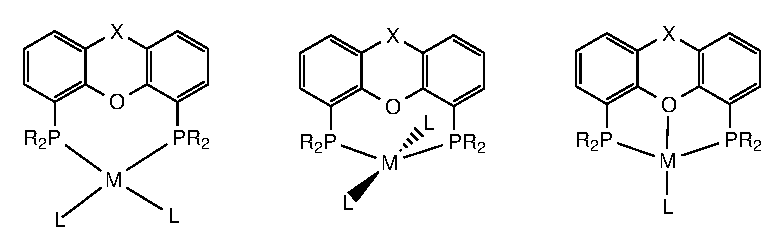
\includegraphics{../Figures/Bondingmodes.eps}
%\caption[Different bonding modes of xantphos ligands]{Different bonding modes of xantphos ligands}
%\vspace{0.2cm}
%\label{Bondingmodes}
%\end{center}
%\end{figure}
%\vspace{0.2cm}
%%
%%\chapter{Introduction}
%%\label{ch:introduction}
%%
%%It is now widely accepted that climate change is occurring at an unprecedented rate.\cite{Oreskes2004}  The concentration of greenhouse gases such as carbon dioxide, methane and nitrous oxide in the atmosphere has been increasing since the industrial revolution (Figure~\ref{Greenhousegases})\cite{Jacobs1999}.  In addition, new greenhouse gases such as \glspl{CFC} are also accumulating in the atmosphere.  \cite{Jacobs1999}  Energy from the sun is absorbed by the surface of the earth and then radiated out into the atmosphere at wavelengths between 5 and 50 \SI{}{\micro\metre}.  Much of this energy is absorbed by atmospheric gases such as ozone and water vapour, however there is a small ``atmospheric window'' between 8 and 13 \SI{}{\micro\metre} where energy can escape into the solar system.  Greenhouse gases in the atmosphere absorb energy in this atmospheric window and rather than letting the energy escape into the solar system, it is radiated back towards earth.\cite{Hardy2003}  As such, the increased atmospheric greenhouse gas concentrations lead to increases in global temperature.\cite{Jacobs1999}
%%
%%Carbon dioxide absorbs strongly above 10 \SI{}{\micro\metre} making it a potent greenhouse gas.\cite{Goody1951}  Prior to the industrial revolution, the amount of carbon dioxide released into the atmosphere was balanced by the amount taken up by natural sinks such as the oceans and the biosphere.  However, the burning of fossil fuels has increased the amount of carbon dioxide released into the atmosphere.  As the carbon in the fossil fuels has been effectively removed from the natural carbon cycle for millennia, the natural sinks for carbon dioxide (biosphere and oceans) have been unable to cope with the increase in concentration resulting in accumulation within the atmosphere.\cite{Jacobs1999}
%%
%%\begin{figure}[h]  
%%\centering
%%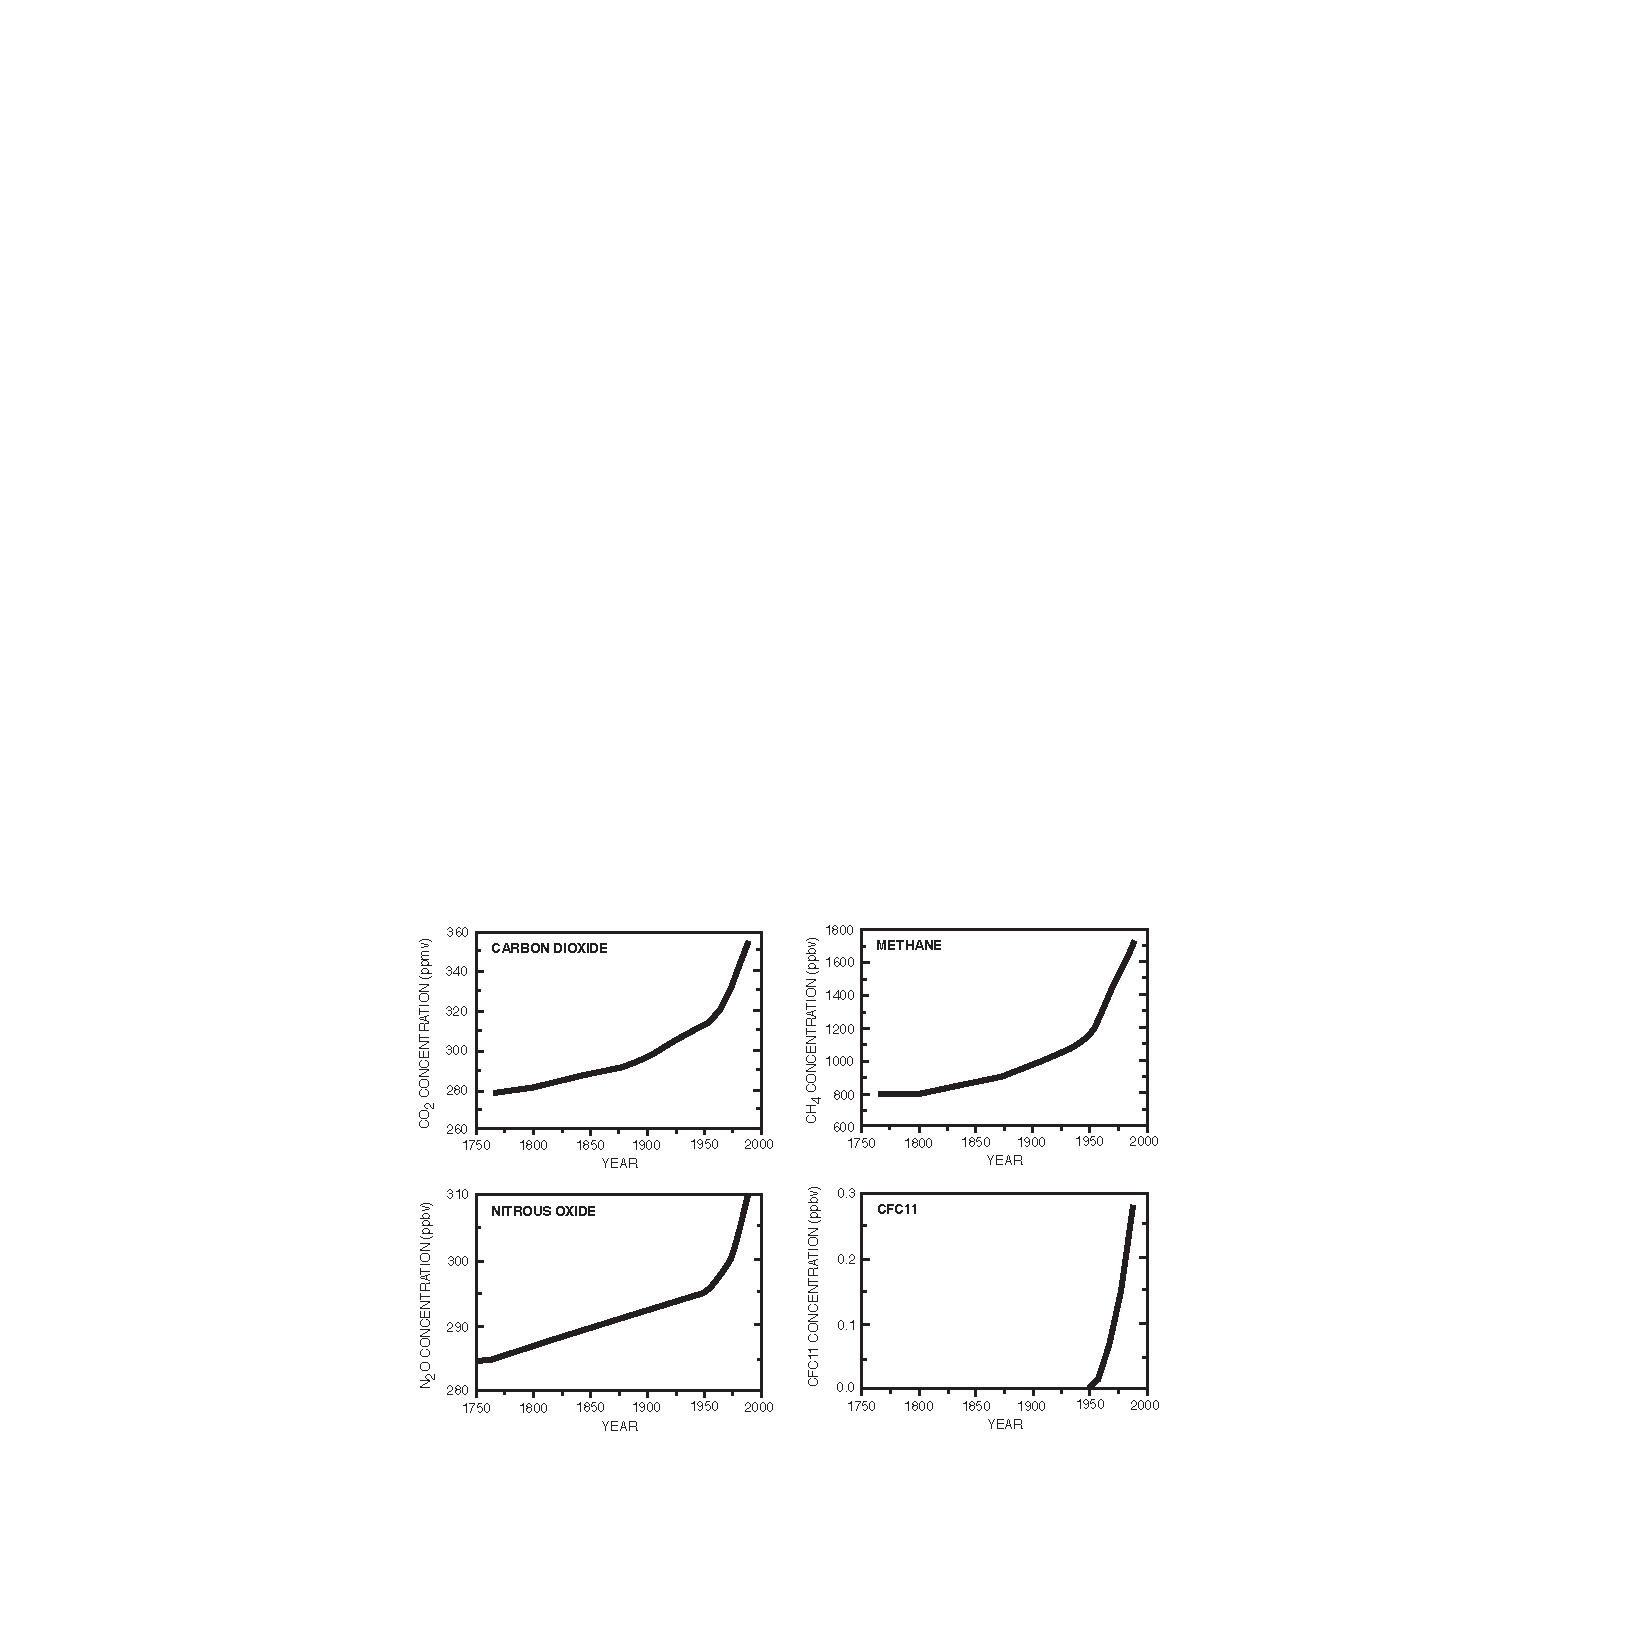
\includegraphics[width = \textwidth]{../Figures/Greenhousegases.pdf}
%%\caption[Concentration of greenhouse gases]{Rise in concentration of greenhouse gases since the 18th century.  Reproduced from \emph{Introduction to Atmospheric Chemistry} p. 113.\cite{Jacobs1999}}
%%\label{Greenhousegases}
%%\end{figure}
%%
%%Fossil fuels are also a prominent source of chemical feedstocks.\cite{Shilov1997}  The alkanes can be converted into alkenes and alkynes \emph{via} hydrothermal cracking and these can be oxidised or otherwise converted to form useful chemical starting materials.  However, the hydrothermal cracking is highly inefficient requiring high temperatures and producing a large range of undesirable by-products.\cite{Shilov1997}  The potential environmental damage from using fossil fuels, together with the mounting costs associated with their extraction, means alternative chemical feedstocks are desirable both environmentally and economically.\cite{Poliakoff2002, Crabtree2011b}
%%
%%Biogas is a mixture of gases containing primarily methane and carbon dioxide with small amounts of hydrogen sulfide, ammonia and other impurities.\cite{Abatzoglou2009}  Generated by the anaerobic digestion of wet organic waste, biogas is considered carbon neutral as the carbon in the organic matter, which is converted to the biogas, is already within the carbon cycle.\cite{Amon2007}  New Zealand has a number of plants to capture the biogas produced from landfill, sewage, farm and food waste.\fixme{cite(Biogas)}  Typically the biogas collected is used for on-site electricity production or co-generation of electricity and methane.
%%
%%%\begin{table}
%%%\caption[Biogas generation sites in New Zealand]{Biogas generation sites in New Zealand}
%%%\label{Biogas}
%%    %\begin{tabular}{l p{4cm} l l}
%%    %\hline
%%%Project name & Feedstock & Application & Year Commissioned\\ \hline
%%%PNCC digester upgrade & Co-digestion & Co-generation & 2008/10\\ 
%%%HCC Digester upgrade (Hamilton) & Co-digestion & Co-generation & projected\\ 
%%%Beef feedlot manure (Waikato)	& Feedlot waste & Study & 2008\\ 
%%%Piggery feedlot manure (Waikato)& Feedlot waste & Study & 2008\\
%%%Chicken Waste (Waikato)	& Industrial & Study / Research & 2008\\ 
%%%Tirau Dairy (Tirau) & Industrial waste & Boilers & 1990\\
%%%Southern Landfill, Happy Valley & Landfill & Power generation & 2008\\
%%%Silverstream (Lower Hutt)	& Landfill & Power generation & 1994\\
%%%Greenmount & Landfill & Power generation & 1992\\ 
%%%Rosedale & Landfill & Power generation & 1994\\
%%%Horotiu Landfill & Landfill & Power generation & 2004\\
%%%Spicer Landfill (Porirua/Wellington) & Landfill & Flaring & 2009 \\ 
%%%Burwood Landfill & Landfill & Co-generation & 2007\\
%%%Tirohia Landfill	& Landfill & Power generation & 2008\\
%%%Hampton Downs Landfill & Landfill & Power generation &2009\\
%%%Landcorp (Waimakariri/Rangiora) & Manure biosolids & Co-generation & 2007/08\\
%%%Kiwifruit Waste (Tauranga) & Rural waste & Study & 2008 \\
%%%Piggery Waste (Canterbury) & Rural waste & Study	& 2008\\ 
%%%Piggery Waste (Waikato)	& Rural waste & Research & 2008\\ 
%%%Piggery Waste (Canterbury) & Rural waste & Study & 2009\\ 
%%%Mangere WWTP I(Auckland) & Sewage & Co-generation	& 2004\\ 
%%%Hamilton WWTP (Hamilton ) & Sewage & Co-generation	& 2005\\
%%%Bromley WWTP & Sewage & Co-generation & 1996\\ 
%%%Tauranga WWTP & Sewage & Co-generation & 1996\\ 
%%%CCC digester upgrade (Christchurch) & Thermophilic / biosolids & Co-generation & projected\\
%%%GI digester (Dunedin) & Thermophilic / biosolids & Boilers & 2001\\
%%    %\hline
%%    %\end{tabular} \end{table}
%%
%%Biogas also has the potential to act as a chemical feedstock for industrial processes that typically use components extracted from crude oil.\cite{Poliakoff2002}  However, there are several issues associated with the use of biogas as a chemical feedstock.  Biogas is often produced at remote sites and as it mostly contains methane, it cannot be transported economically,\cite{Crabtree2001} hence on-site conversion of the methane into a readily transportable liquid such as methanol would reduce the transportation costs considerably.  However methane, like other alkanes, is unreactive towards most chemical transformations.  Although methane can be oxidised, the low reactivity means that severe conditions or highly active reagents are required.  The methanol that is produced is more easily oxidised than methane so over-oxidation to the undesirable carbon dioxide occurs readily. \cite{Crabtree2001}  
%%
%%One of the most commonly used processes to form methanol from methane is the syngas process.  This first converts the methane to carbon monoxide, then reduces it to methanol.  The formation of synthesis gas (Equation \ref{syngasequation}) is carried out over a heterogeneous nickel catalyst and requires pressures of 40 atm and high temperatures of 850 \degrees C.  This is followed by reaction over a mixture of copper, zinc oxide and alumina at 50 - 100 atm and 250 \degrees C (Equation \ref{syngasequation2}). The process is inefficient as the methane is over-oxidised before being reduced to methanol\cite{Crabtree2001} and although the production of synthesis gas yields three moles of hydrogen, only two of these are used in the production of methanol.  The addition of \ce{CO2} to the system allows for reaction of the excess hydrogen to produce methanol and water (Equation \ref{syngasequation3}).
%%
%%\vspace{-1cm}
%%\begin{align}
%%\ce{CH4 + H2O} & \longrightarrow \ce{CO + 3H2} \label{syngasequation} \\[0.5cm]
%%\ce{CO + 2H2} & \longrightarrow \ce{CH3OH} \label{syngasequation2} \\[0.5cm]
%%\ce{CO2 + 3H2} & \longrightarrow \ce{CH3OH + H2O} \label{syngasequation3}
%%\end{align}
%%\vspace{-2cm}
%%%Green chemistry aspect\\
%%%CO2 harming the atmosphere\\
%%%Carbon cycle\\
%%%QC comic http://questionablecontent.net/view.php?comic=1939\\
%%
%%\section{C-H activation}
%%
%%Carbon-hydrogen bonds are among the least reactive bonds as evidenced by their presence in all organic molecules.\cite{Shilov1997}  Indeed the old name for alkanes ``paraffins'' is derived from the Latin \emph{parum affinis} meaning without affinity.  Alkanes have also been referred to as the ``noble gases of organic chemistry.''\cite{Shilov1997}  The carbon-hydrogen bond is considered to be a very strong bond with a bond dissociation enthalpy of 438~kJmol$^{-1}$ for methane.\fixme{cite
%%(SI2002)}  This compares to an average carbon-oxygen bond of 358~kJmol$^{-1}$, and a carbon-carbon single bond of 346~kJmol$^{-1}$.\fixme{cite(SI2002)}  In addition, alkanes have very high ionisation potentials and pK\sub{a} values, and low proton affinities.\cite{Shilov2000}  Alkenes typically have stronger C-H bonds than alkanes, for example ethene and ethyne have bond dissociation enthalpies of 444 and 502 kJmol$^{-1}$ respectively, compared to 410 kJmol$^{-1}$ for ethane.\cite{Shilov1997}  However, the reduced steric hindrance in alkenes leads to greater kinetic reactivity, and stronger aryl-metal bonds result in a thermodynamic driving force for the C-H activation to occur.\cite{Crabtree2001}
%%
%%%bond lengths 1.08 C-H, 1.43 C-O, 1.54 C-C
%%
%%%Ethene, ethyne and benzene all have stronger C-H bonds of 444, 502 and 456 .\cite{Shilov1997}  As such, a carbon-hydrogen bond in an alkane is unlikely to react without strong reagents or severe conditions.\cite{Crabtree2001}
%%
%%C-H activation refers to the increased reactivity of carbon hydrogen bonds that occurs as a result of interaction with another reagent.\cite{Crabtree2001}  Functionalisation involves the replacement of the C-H bond with another functional group (X) to form a C-X bond.  This reaction may occur in a number of different ways depending on the reactivity of the metal complex.\cite{Shilov2000}  Activation is typically easier than functionalisation as the metal alkyl and hydride often recombine \emph{via} reductive elimination during attempts to functionalise.\cite{Crabtree2001}  
%%%However, the functionalisation is crucial for the conversion of methane to a useful feedstock.
%%
%%%The functionalisation step may be viewed as a organic reaction occuring on a metal support which is important for the activation of the bond.\fixme{reword this?}  
%%
%%%This is essentially an organic reaction following activation.\cite{Crabtree2001}  
%%
%%There are three main processes by which C-H activation can occur.\cite{Shilov2000}  The first is the organometallic activation which involves the formation of a metal-carbon bond.  This may involve cleavage of the bond through either oxidative addition (Equation \ref{Oxidativeequation}) or electrophilic substitution (Equation \ref{Electrophilicequation})  In the second type the alkane C-H bond interacts with a ligand on the metal rather than the metal itself (Equation \ref{Oxidationequation}).  The third type involves the generation of a reactive species by the metal complex, which then attacks the C-H bond (Equation \ref{Radicalequation}).  Systems where organometallic activation occurs will be the focus of this proposal.
%%
%%\vspace{-1cm}
%%\begin{align}
%%\ce{RH + M}^{n+}	& \longrightarrow	\ce{[R-M-H]}^{n+2} \label{Oxidativeequation} \\[0.5cm]
%%\ce{RH + M}^{n+}	& \longrightarrow	\ce{R-M}^{(n+2)+} + \ce{H+} \label{Electrophilicequation} \\[0.5cm]
%%\ce{RH + O=M}^{n+} 	& \longrightarrow	\ce{R\dot} + \ce{HO-M}^{(n-1)+} \label{Oxidationequation} \\[0.5cm]
%%\ce{H2O2 + Fe}^{2+}	 & \longrightarrow	\ce{HO\dot{} + HO- + Fe}^{3+} \label{Radicalequation} \\
%%\ce{HO\dot} + \ce{RH} & \longrightarrow	\ce{H2O + R\dot} \notag \\[0.5cm]
%%\ce{CH4 + 2O2} & \longrightarrow \ce{CO2 + 2H2O} \label{Combustion}
%%\end{align}
%%
%%%\fixme{similarities between C-H and H-H activation}
%%
%%Alkanes can react at elevated temperature with oxygen in the atmosphere to form the thermodynamically stable products water and carbon dioxide (Equation \ref{Combustion}).  However, alkanes are inert in air at room temperature in the absence of a catalyst.\cite{Shilov1997}  Alkanes can be converted into other hydrocarbons by heating.  This forms radical species which can combine to form longer or shorter chain alkanes, alkenes and alkynes.\cite{Sironi1990}  For example, methane may be converted into ethane, ethene and ethyne by heating at temperatures in excess of 900 \degrees C.\cite{Shilov1997}  Alkanes can also be protonated by superacids, leading to elimination of hydrogen gas, giving an overall hydride abstraction reaction.  However, the elimination occurs selectively with the most basic hydride and the superacids used will attack a number of functional groups.\cite{Crabtree2004}
%%
%%%\vspace{-0.8 cm}
%%%\begin{equation}
%%
%%%\label{Combustion}
%%%\end{equation}
%%
%%The presence of other functional groups on the molecule can result in activation of a C-H bond.  A common example of this is protons $\alpha$ to a carbonyl group that are easily removed in the presence of a base.  This forms the basis for a number of widely utilised organic reactions such as the aldol condensation reaction (Scheme~\ref{Aldolcondensation})\cite{Saito2004}.  However in alkanes, no functional groups are present to activate the bond so it is necessary to activate the bond using an external source such as an enzyme or coordination complex.\cite{Crabtree2001}
%%
%%\begin{scheme}[h]  
%%  \centering
%%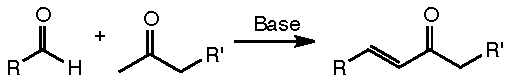
\includegraphics[]{../Schemes/Aldolcondensation.pdf}
%% \caption[Aldol condensation reaction]{Aldol condensation reaction}
%% \label{Aldolcondensation}
%%\end{scheme}
%%
%%%104 kcal mol-1 = ~435 kJmol-1
%%
%%Complex organic molecules are synthetic targets as a result of their potential use as pharmaceuticals.  Currently the synthesis of these target molecules relies on the modification of existing functional groups.  The regio- and stereo-selective activation and functionalisation of C-H bonds within complex organic molecules would result in a major paradigm shift in organic synthesis.\cite{Davies2008}
%%
%%\subsection{Biological systems}
%%
%%As previously discussed, the oxidation of methane to methanol without over-oxidation to carbon dioxide is desirable in order to make use of biogas as a chemical feedstock.\cite{Crabtree2001}  Like many other desirable chemical transformations, enzymes exist that are capable of performing the reaction.  Methane monooxygenase and cytochrome P450 catalyse the oxidation of alkanes to alcohols (Equation \ref{Methanemonooxygenaseequation}).\cite{Crabtree1995}  Although methane monooxygenase is specfic for methane, cytochrome P450 enzymes will catalyse the oxidation of a range of alkanes.\cite{Lipscomb1994, Crabtree2001}
%%
%%\vspace{-0.8 cm}
%%\begin{equation}
%%\ce{NADPH + O2 + RH + H+} \longrightarrow \ce{NADP+ + H2O + ROH}
%%\label{Methanemonooxygenaseequation}
%%\end{equation}
%%
%%Methane monooxygenase is found in bacteria that exist at the interface of aerobic and anaerobic environments found in lakes, oceans and soils.\cite{Lipscomb1994}  These bacteria are described as methanotrophic, they utilise methane as their source of carbon and energy.\cite{Haber1983}  Methane monooxygenase consists of three proteins; component B, reductase and hydroxylase.\cite{Lipscomb1994}  The hydroxylase protein contains a dinuclear iron centre that activates oxygen to form an oxo-bridged system.  This reacts with methane to give methanol and a hydroxo-bridged diiron centre.\cite{Merkx2001}  However, despite numerous studies,\cite{Lipscomb1994, Merkx2001, Tinberg2011} the mechanism of methane monooxygenase has proved elusive with a number of different mechanisms proposed (Scheme \ref{Methanemonooxygenasemechanism}).
%%
%%%The hydroxylase protein contains a hydroxo-bridged dinuclear iron that forms that active catalytic site.  Both iron atoms are reduced to Fe(II) and then react with \ce{O2} The O-O bond is cleaved to give water and a Fe(IV)Fe(IV)=O species which can abstract a hydrogen from methane.  This gives an OH radical and a \ce{CH3} radical which recombine to form methanol.\fixme{SCHEME}
%%
%%%\begin{figure}[h]
%%%\centering
%%%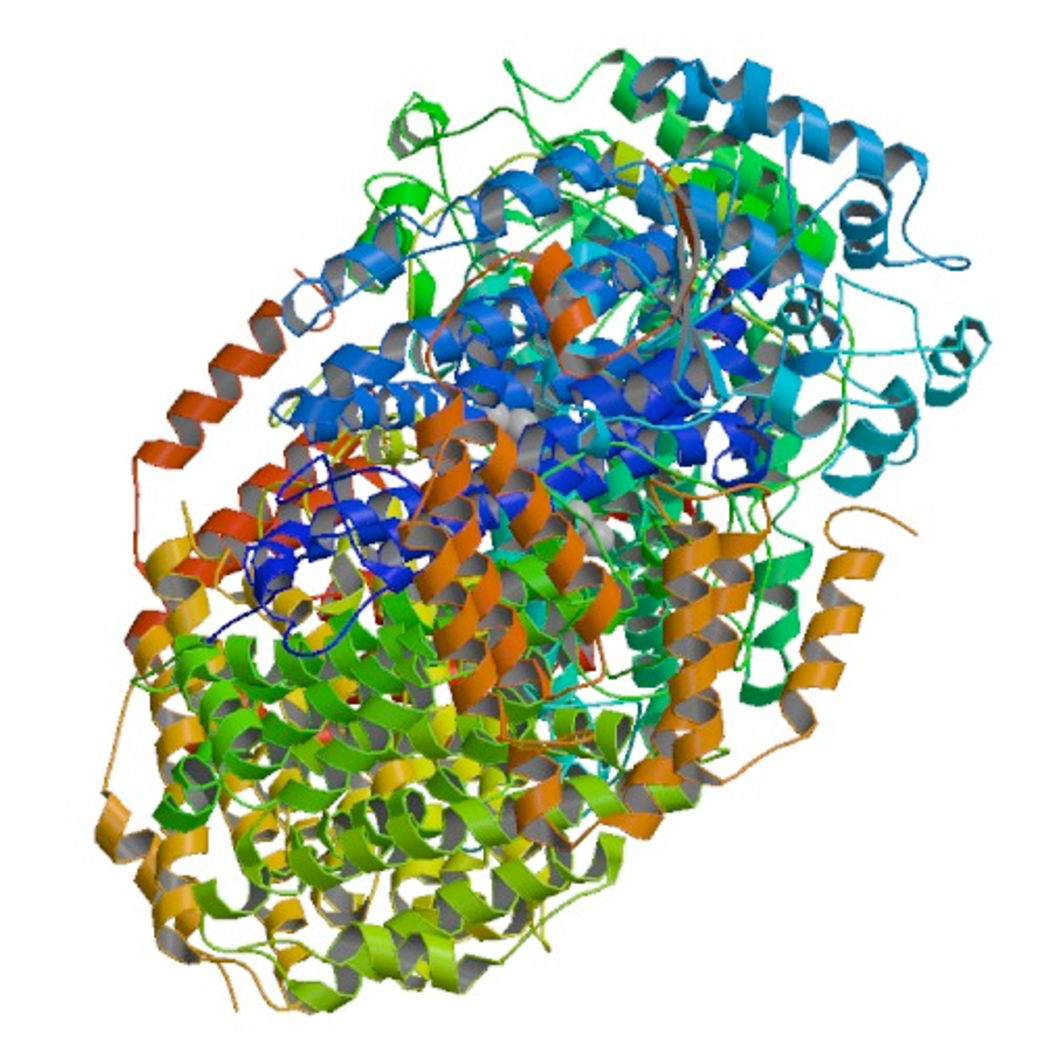
\includegraphics[height = 5cm]{../Figures/Methanemonooxygenase.pdf}
%%%\caption[X-ray crystal structure of methane monooxygenase]{X-ray crystal structure of methane monooxygenase reproduced from \fixme{reference from protein databank}}
%%%\label{Methanemonooxygenase}
%%%\end{figure}
%%
%%\begin{scheme}[h]
%%\centering
%%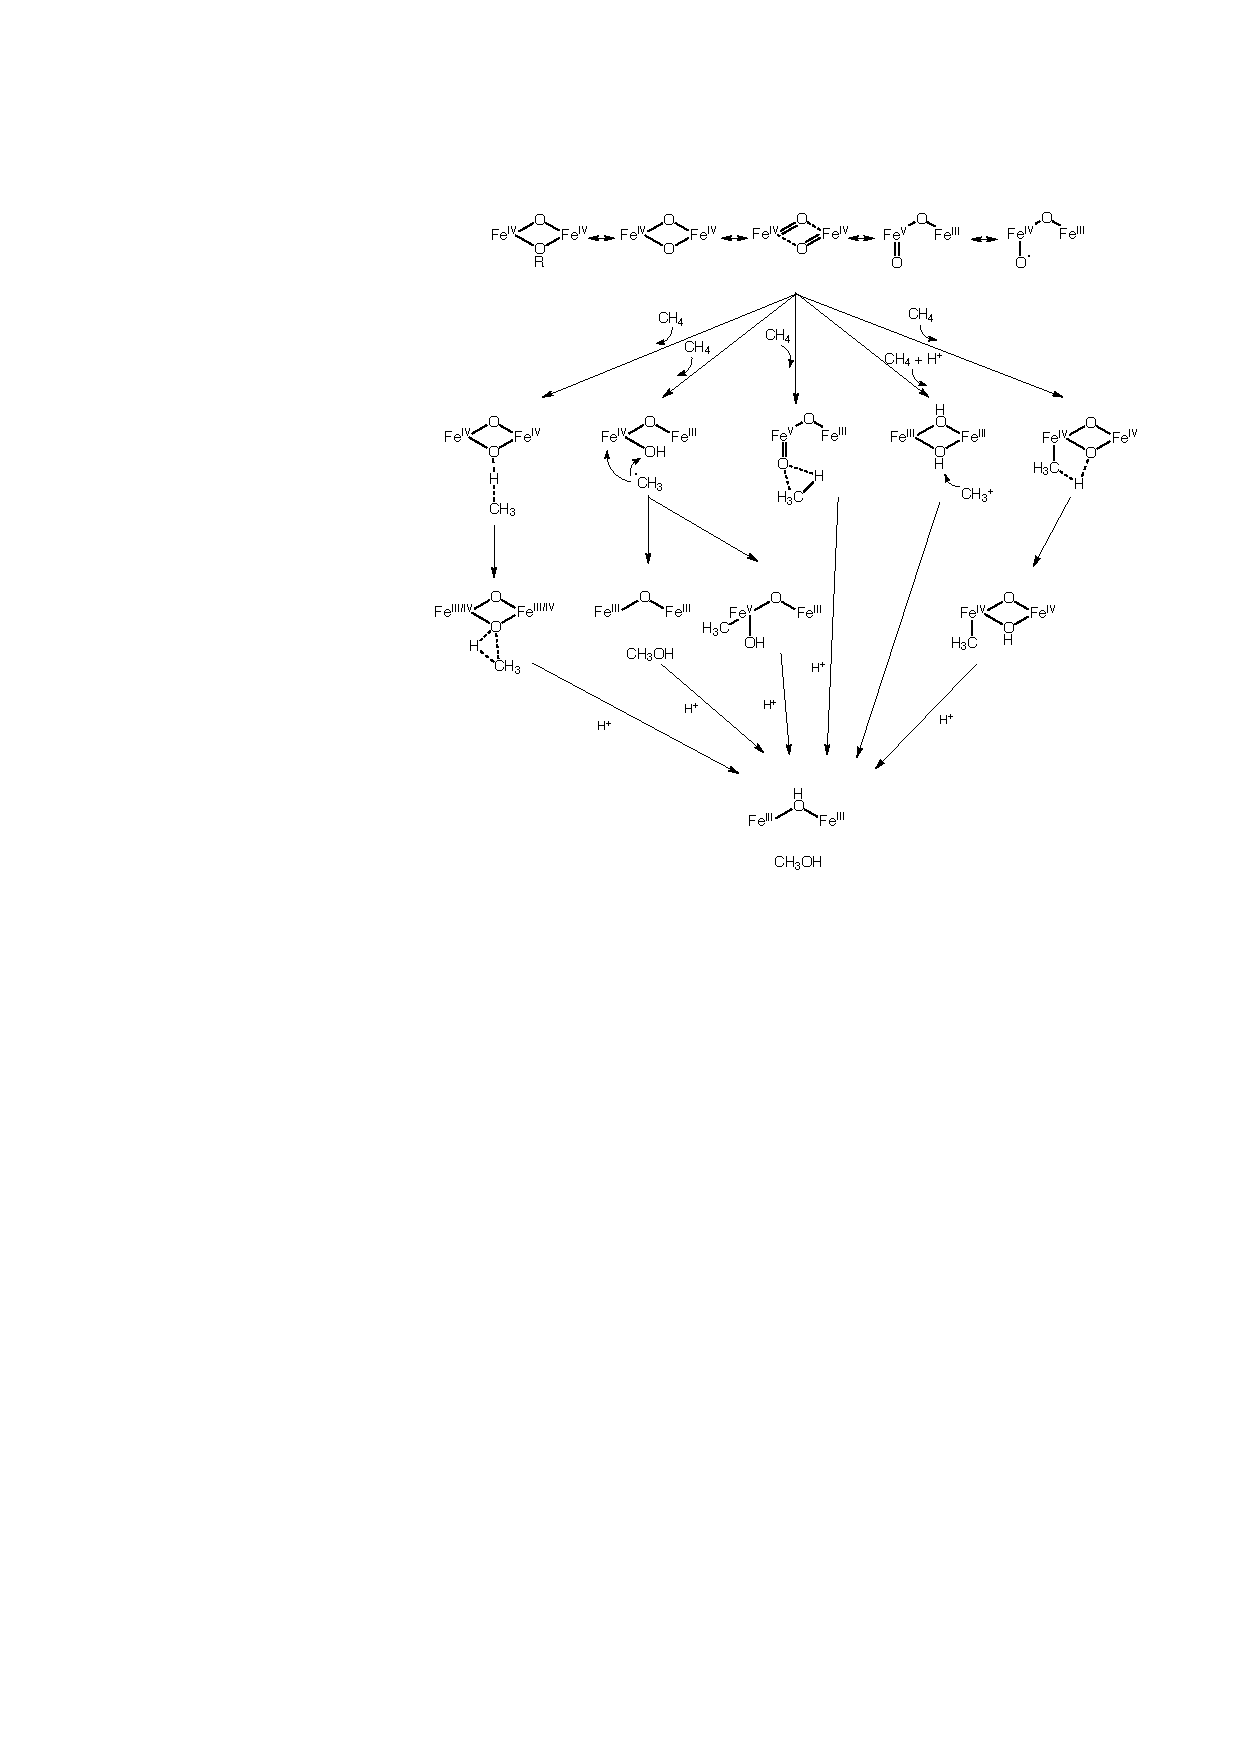
\includegraphics[width = 0.95\textwidth]{../Schemes/Methanemonooxygenasemechanism.pdf}
%%\caption[Proposed mechanisms for the hydroxylation of methane]{Proposed mechanisms for the hydroxylation of methane reproduced from Lippard et al.\cite{Merkx2001}}
%%\label{Methanemonooxygenasemechanism}
%%\end{scheme}
%%
%%Cytochrome P450 enzymes are found in a most classes of organisms including bacteria, fungi, plants, insects and mammals.\cite{Montellano2010}  The consistent feature across all P450 enzymes is the presence of a heme group with a coordinated thiolate ion at the active site of the molecule.\cite{Montellano2010}  The first step in metabolism of pharmaceuticals in the body, phase 1, typically involves oxidation, reduction and hydrolysis reactions.  P450 enzymes are responsible for the phase 1 metabolism of around 75\% of known pharmaceuticals.\cite{Rittle2010}  Although the enzymes perform a number of roles, one of the most interesting is the hydroxylation of C-H bonds.\cite{Rittle2010}
%%
%%The overall catalytic cycle for the hydroxylation of an alkane by a P450 enzyme reported by de Montellano\cite{Montellano2010} is given in Scheme \ref{P450catalyticcycle}.  In the resting state (A) the Fe(III) is bound to a thiolate and the \emph{trans} ligand is typically a water molecule though some P450's do not have a \emph{trans} ligand.  The water is displaced upon binding of an RH group.  Binding of the RH allows electron transfer to occur, reducing the Fe(III) to Fe(II) (C).  Oxygen binds to the Fe(II) resulting in the superoxide complex D.  This undergoes electron transfer and protonation to form the hydroperoxo complex E.  This complex is protonated and undergoes loss of \ce{H2O} to form the porphyrin radical cation F.  F can then react with the substrate to give the alcohol product.  Following product release and rebinding of water the resting state is restored.
%%
%%%\begin{figure}[h]
%%%\centering
%%%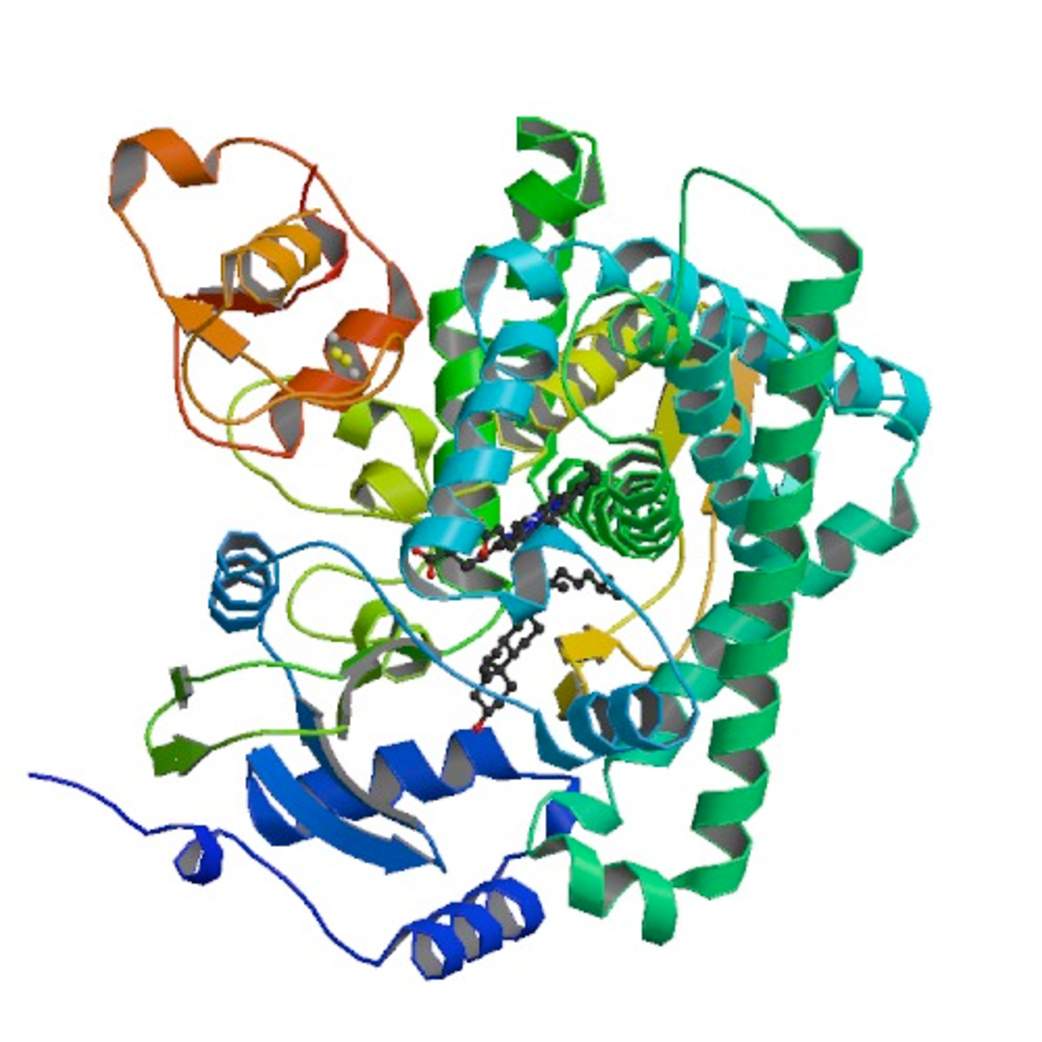
\includegraphics[height = 5cm]{../Figures/P450.pdf}
%%%\caption[X-ray crystal structure of P450]{X-ray crystal structure of P450 reproduced from \fixme{reference from protein databank}}
%%%\label{P450}
%%%\end{figure}
%%
%%\begin{scheme}[ht]
%%\centering
%%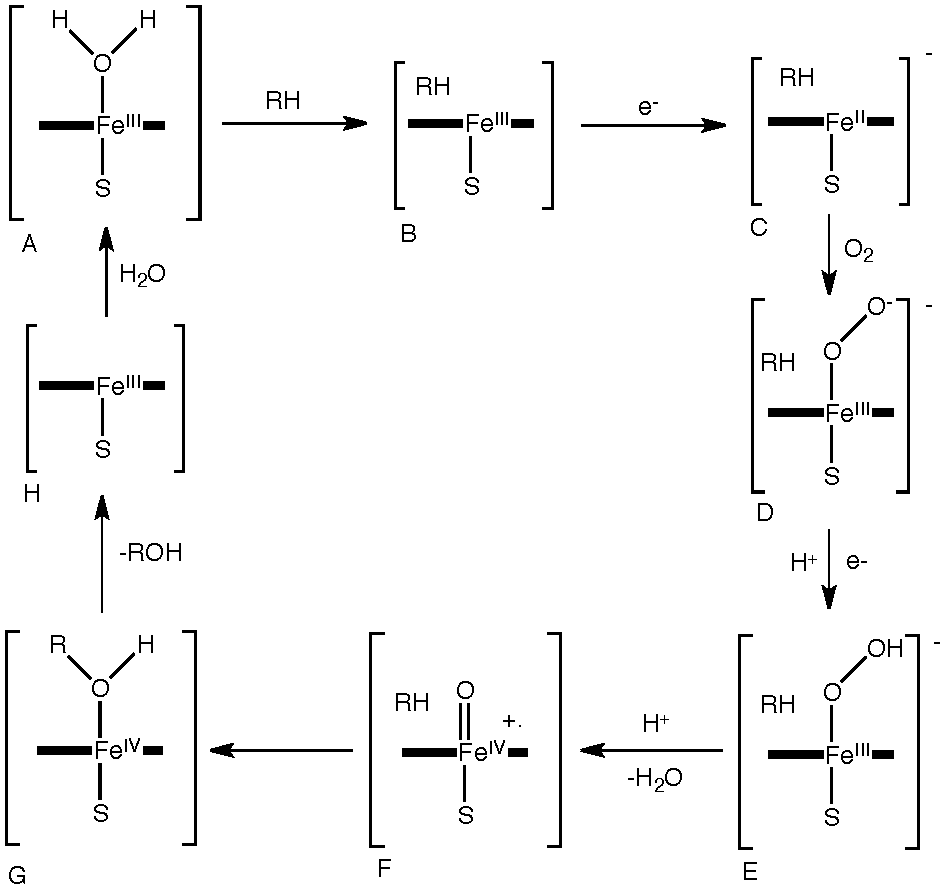
\includegraphics[width = 0.75\textwidth]{../Schemes/P450catalyticcycle.pdf}
%%\caption[Proposed catalytic cycle for hydroxylation by P450]{Proposed catalytic cycle for hydroxylation by P450 reported by de Montellano\cite{Montellano2010}}
%%\label{P450catalyticcycle}
%%\end{scheme}
%%
%%\subsection{Organometallic systems}
%%
%%There are a number of different types of bonds that can form in organometallic systems (Figure \ref{Bondingmodesintro}).  The most common is the donation of a ligand lone pair of electrons to a vacant orbital on the metal (a).  This is typically observed for ligands such as \ce{PR3,~CH3^-~and~H2O} among many others.  Donation of a $\pi$-bonding pair of electrons to the metal (b) is also common, typically among the alkene complexes such as those with ethene.  There are a number of rarer bonding forms including the donation of a $\sigma$-bonding pair of electrons (c) and the alkyl agostic interaction (d).\cite{Bernskoetter2009}  In addition, the metal can donate electron density from filled d orbitals into the LUMO of the ligand (either the $\sigma$* or $\pi$* orbital).\cite{Chatt1955}
%%
%%\begin{figure}[ht]
%%\centering
%%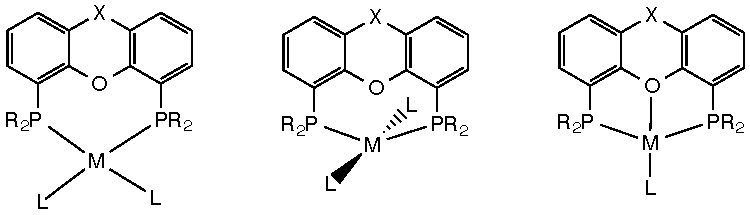
\includegraphics[width = 0.5\textwidth]{../Figures/Bondingmodes.pdf}
%%\caption[Bonding in organometallic complexes]{Bonding in organometallic complexes}
%%\label{Bondingmodesintro}
%%\end{figure}
%%
%%Alkanes are weak $\sigma$-bases and $\pi$-acids.  As such they are very poor ligands for transition metals.\cite{Crabtree1993}  Typically alkanes form $\sigma$-complexes with metals that can $\pi$-backbond.  For successful complexation a low valent metal and the absence of competitive decomposition pathways are required.\cite{Crabtree2001}  Enhanced bonding of alkanes occurs with metals capable of forming enhanced $\pi$-backbonding into the $\sigma$* C-H orbital, similar to that found for molecular hydrogen complexes.\cite{Kubas1988}
%%
%%The activation of C-H bonds is thought occur \emph{via} a stepwise process involving the coordination of the alkane to the metal to form a $\sigma$-complex, followed by the oxidative cleavage of the C-H bond forming metal-alkyl and metal-hydride bonds.\cite{Labinger2002}  The intermediate  $\sigma$-complexes are highly unstable and until recently their existence had only been inferred by isotope scrambling and the inverse kinetic isotope effect in reductive elimination reactions of alkyl hydrides.\cite{Bernskoetter2009, Labinger2002}  In 2009 Brookhart reported the characterisation of a relatively long-lived rhodium(I) $\sigma$-methane complex.\cite{Bernskoetter2009}  The complex was formed by the protonation of a rhodium methyl complex (Scheme \ref{Sigmamethane}).  At -87~\degrees C the methane is displaced by solvent (\ce{CDCl2F}) with a half-life of 83 minutes.
%%
%%\begin{scheme}[ht]
%%\centering
%%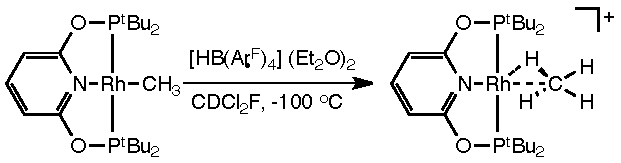
\includegraphics[]{../Schemes/Sigmamethane.pdf}
%%\caption[Formation of a $\sigma$-methane complex]{Formation of a $\sigma$-methane complex.  Ar\ce{^{F}} = \emph{m}-di(trifluoromethyl)phenyl}
%%\label{Sigmamethane}
%%\end{scheme}
%%
%%%$\sigma$-Complexes of methane have been proposed 
%%%The first example of C-H activation was reported by Dimroth in 1902\cite{Dimroth1902}  Reaction of phenol with a solution of mercury acetate on a steam bath replaced the \emph{ortho} and \emph{para}-protons with a mercury acetate group.  \fixme{more info etc}
%%
%%C-H activation has developed significantly since the first example of C-H activation by an organometallic complex was reported by Chatt in 1962. \cite{Chatt1962}  Reduction of metal halides by sodium napthalene in the presence of an excess of \gls{dmpe} produced V, Cr, Mo and W complexes of the form \ce{[M(}\gls{dmpe}\ce{)_3]},  and Fe and Co complexes of the form \ce{[M(}\gls{dmpe}\ce{)_2]}.  However, the \ce{[Ru(}\gls{dmpe}\ce{)_2]} analogue gave a hydride complex ``by taking hydrogen from the napthalene.''\cite{Chatt1962}  
%%
%%Further analysis of the ruthenium system was carried out and published in 1965.\cite{Chatt1965} Reaction of \emph{cis}- or \emph{trans}-\ce{[RuCl2(}\gls{dmpe}\ce{)_2]} with benzene, naphthalene, anthracene and phenylanthracene formed the \emph{cis}-\ce{[RuH(aryl)(}\gls{dmpe}\ce{)_2]} (aryl = phenyl, naphthyl, anthryl and phenanthryl) complexes \emph{via} oxidative addition.\cite{Chatt1965}  The activation is reversible, as reactions of the complexes with hydrochloric acid yielded hydrogen gas, the aromatic starting material and \emph{cis}-\ce{[RuCl2(}\gls{dmpe}\ce{)_2]} (Equation \ref{ChattCH}).  The C-H activation to form the complexes was selective for example, in the reaction with naphthalene the activation occurred exclusively at the 2-position.
%%
%%\vspace{-0.6 cm}
%%\begin{equation}
%%\ce{[RuH(C10H7)(dmpe)2] + 2HCl} \longrightarrow \ce{[RuCl2(dmpe)2] + H2 + C10H8}
%%\label{ChattCH}
%%\end{equation}
%%
%%The naphthyl hydride complex formed by treatment of \ce{[Ru(}\gls{dmpe}\ce{)_2]} with naphthalene thermally decomposed giving a complex with properties consistent with \ce{[Ru(}\gls{dmpe}\ce{)_2]} (Scheme \ref{Chattdmpescheme}).\cite{Chatt1965}  However, infrared spectroscopy showed a signal for a Ru-H at 1791 \percm,  leading to the proposed structure of \ce{[RuH(CH2PMeCH2CH2PMe2)(}\gls{dmpe})], formed by activation of a C-H bond from the \gls{dmpe} ligand.\cite{Chatt1965}  X-ray crystallography later allowed the reformulation of the structure to the analogous dimer.\cite{Crabtree2004}  However, this species remains the first example of cyclometallation of an sp$^3$ C-H bond.
%%
%%\begin{scheme}[ht]
%%\centering
%%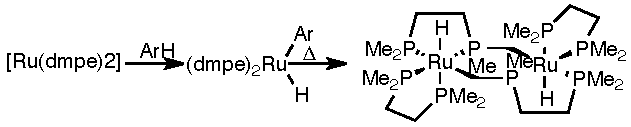
\includegraphics[]{../Schemes/Chattdmpescheme.pdf}
%%\caption[C-H activation reactions reported by Chatt and Davidson]{C-H activation reactions reported by Chatt and Davidson\cite{Chatt1965}}
%%\label{Chattdmpescheme}
%%\end{scheme}
%%
%%The exchange of hydrogen with deuterium in polyalkyl benzenes, polycyclic aromatic hydrocarbons and heterocycles can be catalysed by homogeneous platinum (II) species.\cite{Hodges1968, Hodges1969, Hodges1969b}  Using deutero-acetic acid as a solution in \ce{D2O}, together with DCl or anhydrous tin(IV) chloride to prevent the formation of platinum metal, H/D exchange on the substrate was observed when exposed to \ce{Na2PtCl4} or \ce{K2PtCl4}.\cite{Hodges1968, Hodges1969}  Although the rate of exchange was faster for unhindered aromatic protons, H/D exchange was also observed for alkyl protons.\cite{Hodges1969b}  The rate was fastest for \hbox{\emph{p}-xylene}, \gls{mesitylene}, \emph{m}-xylene and toluene, however exchange of alkyl protons was also observed in \emph{o}-xylene, \gls{hemimellitene} and \gls{durene}.\cite{Hodges1969b}
%%
%%This activation of alkyl protons inspired Shilov to investigate the C-H activation of alkanes by platinum.  The system carries out oxidation of alkanes such as methane \emph{via} electrophilic activation (Scheme \ref{Shilovcatalyticcycle}).\cite{Labinger2002, Crabtree2001}  The first step involves displacement of a chloride ligand on the platinum by a $\sigma$-methyl followed by oxidative addition and loss  of H$^+$ \emph{via} loss of HCl.  The Pt(II) is then  oxidised to Pt(IV) \emph{via} electron transfer to the \ce{PtCl6}$^{2-}$.  Finally, the complexed methyl undergoes nucleophilic attack from water displacing the \emph{trans} chloride ion to form HCl, methanol and regenerate the catalyst.  The system has shown selectivity for terminal C-H bonds.  For example, in the oxidation of ethanol functionalisation occurs at the methyl to yield ethylene glycol (Equation \ref{Ethyleneglycol}) whilst, all other methods of oxidation will oxidise the hydroxyl functionality.\cite{Labinger1993}  This can be utilised for the one-pot synthesis of ethylene glycol from ethanol.\cite{Sen1994}  However, the selectivity is lost in reaction with 2-propanol which gives only acetone.\cite{Labinger1993}
%%\vspace{-1.5cm}
%%\begin{scheme}[ht]
%%\centering
%%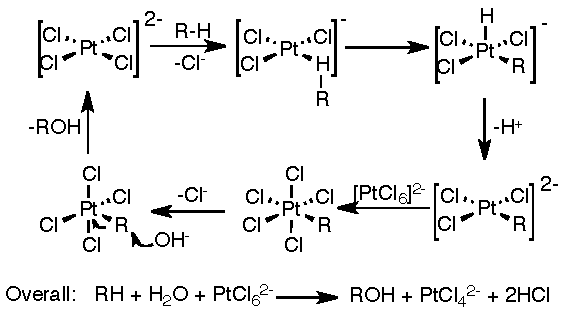
\includegraphics[]{../Schemes/Shilovcatalyticcycle.pdf}
%%\caption[Platinum catalysed oxidation of alkanes]{Platinum catalysed oxidation of alkanes}
%%\label{Shilovcatalyticcycle}
%%\end{scheme}
%%
%%\begin{equation}
%%\ce{CH3CH2OH + H2O + PtCl6}^{2-} \longrightarrow \ce{CH2OHCH2OH + PtCl4}^{2-} + \ce{2HCl} 
%%\label{Ethyleneglycol}
%%\end{equation}
%%
%%Although the Shilov system is catalytic in Pt(II), it requires a stoichiometric amount of Pt(IV).  In addition, the Pt(II) catalyst is unstable in solution and eventually precipitates as platinum metal.\cite{Luinstra1995}  This results in an expensive and thus impractical system for industrial application.  The relatively low yields of the system also reduce its industrial viability.\cite{Periana1993}  Furthermore, the reaction produces two equivalents of hydrochloric acid which require disposal at significant cost.\cite{Poliakoff2001}  A number of attempts have been made to replace the Pt(IV) primary oxidant thus making an economically viable system.\cite{Periana1993, Periana1998, Hashiguchi2010}  However, this has proven challenging as most oxidants tend to convert Pt(II) to the inactive Pt(IV).\cite{Crabtree2001}  Additionally, an oxidant is required that will not attack the product alcohol.  
%%
%%In 1993 Periana reported the use of concentrated sulfuric acid as the primary oxidant and Hg(II) as a catalyst in place of the platinum.\cite{Periana1993}  The Hg(II) is the highest possible oxidation state so further unwanted oxidation of the catalyst is not possible.  Using methane as the feedstock, the system produces methyl bisulfate in a 43\% yield (Scheme \ref{Mercurycatalyticcycle}).  This has the advantage of being highly resistant to oxidation preventing the formation of carbon dioxide. However, the catalysis involves the formation of MeHg(II)$^+$ as an intermediate following activation.  Methyl mercury salts, like most organomercury compounds, are extremely toxic and exhibit accumulation effects in biological systems.\fixme{cite(MethylmercuryMSDS)}  Sulfur dioxide, a significant contributor to acid rain,\cite{Jacobs1999} is also produced as a stoichiometric byproduct of this reaction.  However, the oxidation of sulfur dioxide to sulfuric acid by air is an established industrial process and could be utilised to provide further sulfuric acid for the process.\cite{Periana1993}
%%
%%%\begin{equation}
%%%\ce{CH4 + 2H2SO4} \longrightarrow \ce{CH3OSO3H + 2H2O + SO2} 
%%%\label{Mercuryequation}
%%%\end{equation}
%%
%%%Periana 1993 reaction is carried out at 180 degrees
%%%Periana 1998 reaction is carried out at 100 degrees
%%
%%\begin{scheme}[ht]
%%\centering
%%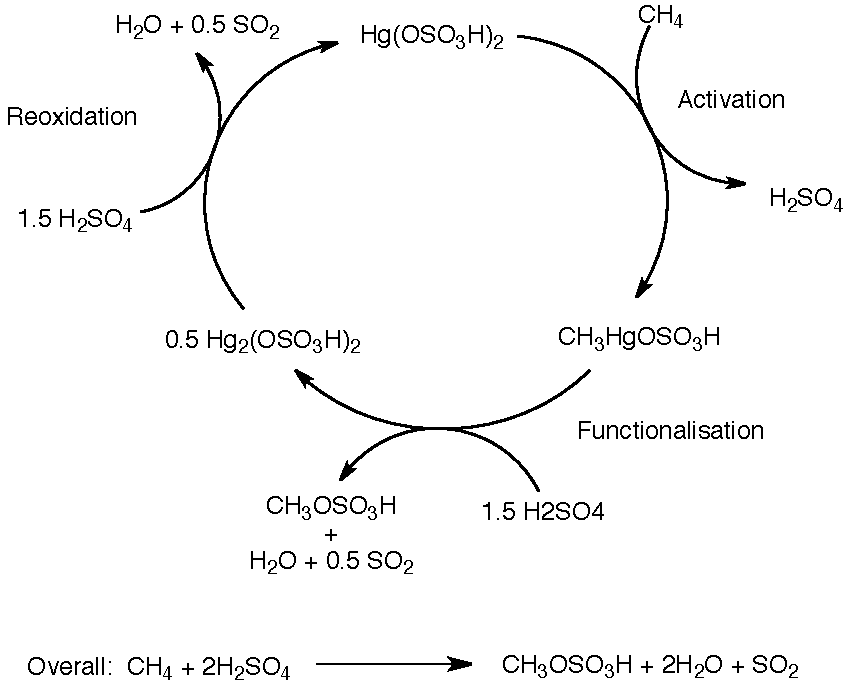
\includegraphics[width = 0.8\textwidth]{../Schemes/Mercurycatalyticcycle.pdf}
%%\caption[Mercury catalysed oxidation of methane]{Mercury catalysed oxidation of methane}
%%\label{Mercurycatalyticcycle}
%%\end{scheme}
%%
%%Further work by Periana investigated changing the Pt(II) system to improve stability, activity and prevent oxidation to Pt(IV).\cite{Periana1998}  Nitrogen donor ligands were utilised as oxygen systems have high kinetic lability on platinum and phosphorus ligands have poor oxidative and thermal stability.  The use of \emph{cis}- or \emph{trans}-\ce{[PtCl2(NH3)2]} in concentrated sulfuric acid at 180~\degrees C gave 90\% selectivity for methyl bisulfate.  However, the catalyst degraded to insoluble \ce{PtCl2} and \ce{NH4HSO4}.  
%%
%%In an extension of this work a $\pi$-acidic chelating donor ligand \gls{bpym} was utilised as $\pi$-donor ligands were expected to have lower proton affinity and form stronger Pt-N bonds than the \ce{NH3} ligands used previously.  The \ce{[PtCl2(}\gls{bpym})] complex was tested in 20 \% \ce{SO3} in \ce{H2SO4} at 200~\degrees C for 50 hours.  Some free ligand and HCl was observed, however the solution remained homogenous showing no formation of platinum metal or other insoluble products.  Using \emph{cis}-\ce{[PtCl2(}\gls{bpym})] in the catalytic system at 220~\degrees C for 2.5 hours resulted in 90\% methane conversion with an 81\% selectivity (carbon dioxide forming the major byproduct).\cite{Periana1998}  However, this reaction requires high temperatures and forms significant amounts of carbon dioxide and sulfur dioxide both of which are environmentally hazardous.\cite{Jacobs1999}  The reaction proceeds \emph{via} a slightly different mechanism to the mercury system (Scheme \ref{PerianaPtcycle}) with oxidation occurring prior to the functionalisation.\cite{Periana1998}
%%
%%%\begin{figure}[h]
%%%\centering
%%%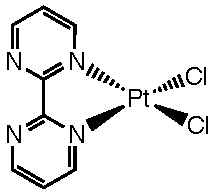
\includegraphics[height = 4cm]{../Figures/bpym.pdf}
%%%\caption[Structure of \ce{[PtCl2(bpym)]}]{Structure of \ce{[PtCl2(bpym)]}}
%%%\label{bpym}
%%%\end{figure}
%%
%%\begin{scheme}[ht]
%%\centering
%%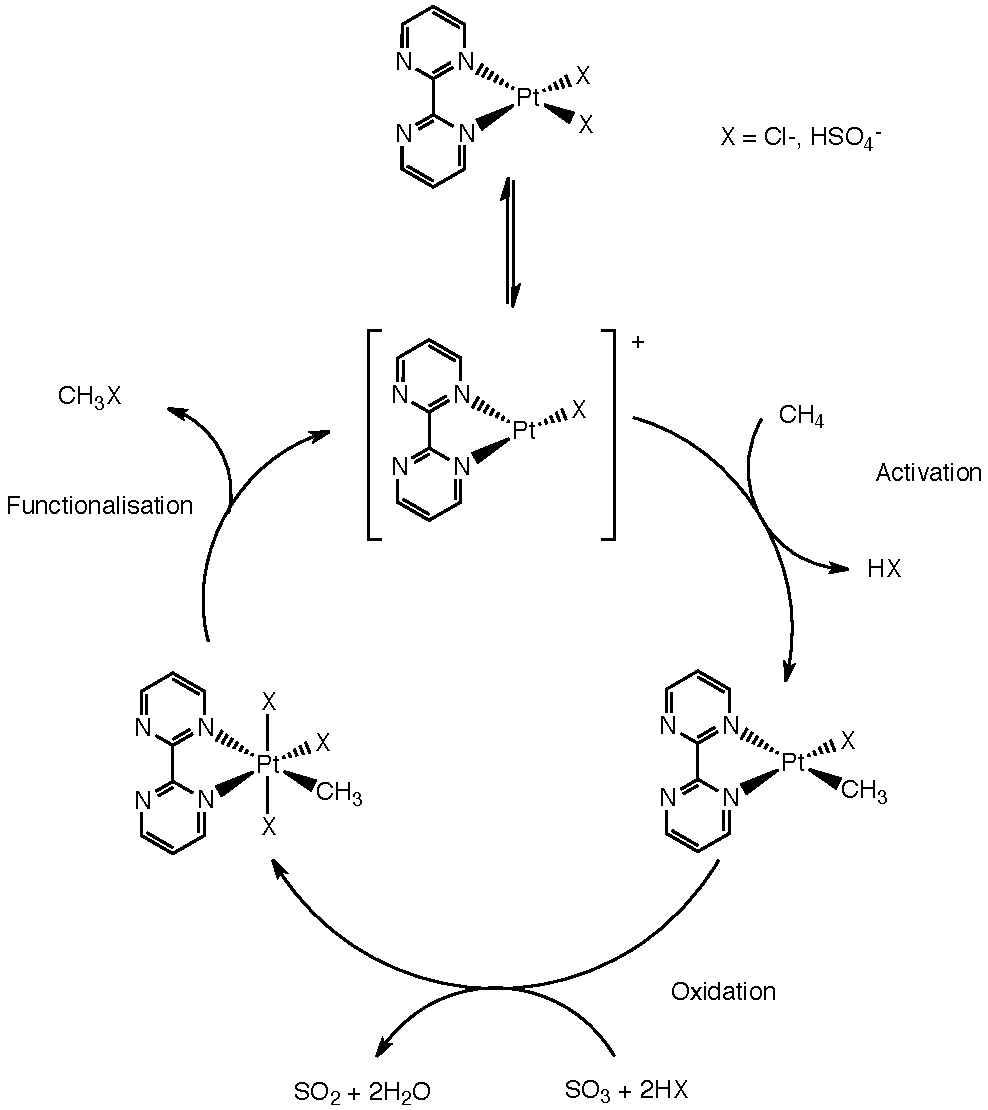
\includegraphics[width = 0.9\textwidth]{../Schemes/PerianaPtcycle.pdf}
%%\caption[Oxidation of methane catalysed by \ce{[PtCl2(bpym)]}]{Oxidation of methane catalysed by \ce{[PtCl2(bpym)]}}
%%\label{PerianaPtcycle}
%%\end{scheme}
%%
%%%Nature of the C-H bond\\ 
%%%Strong\\
%%%Highly non-polar\\
%%%General catalytic attempts\\
%%%Shilov etc.\\
%%
%%\subsection{Alkane dehydrogenation}
%%
%%Alkane dehydrogenation is an alternative approach that combines the activation and functionalisation into a single step.  This methodology was developed from the \hbox{organometallic} complexes such as Wilkinson's\cite{Osborn1966} and Crabtree's\cite{Crabtree1979b} catalysts (Figure \ref{Wilkinsoncrabtree}) that are utilised as homogeneous hydrogenation catalysts.  Wilkinson's catalyst was the first homogeneous hydrogenation catalyst with comparable rates to the heterogeneous counterparts and has become very widely utilised in organic synthesis.\cite{Knowles2003}
%%
%%\begin{figure}[ht]
%%\centering
%%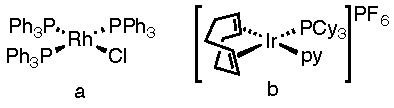
\includegraphics[]{../Figures/Wilkinsoncrabtree.pdf}
%%\caption[Wilkinson's and Crabtree's catalysts]{Wilkinson's (a) and Crabtree's (b) catalysts}
%%\label{Wilkinsoncrabtree}
%%\end{figure}
%%
%%Crabtree reported a number of hydrogenation catalysts based on Wilkinson's catalyst in 1977.\cite{Crabtree1977} The most active of these, \ce{[Ir(cod)(PCy3)(py)]PF6} (Figure \ref{Wilkinsoncrabtree} b, \gls{cod} = 1,5-cyclooctadiene, \gls{Cy}~=~cyclohexyl, \gls{py} = pyridyl) has become known as Crabtree's catalyst.\cite{Cui2005}  This catalyst is active for the hydrogenation of a range of \hbox{mono-,} di-, \hbox{tri-,} and \hbox{tetra-substituted} alkenes with turnover frequencies (\glspl{TOF}) of 6400, 4500, 3800 and 4000 for hex-1-ene, cyclohexene, 1-methylcyclohexene and 2,3-dimethylbut-2-ene respectively.\cite{Crabtree1979b}  Crabtree's catalyst is useful for the hydrogenation of tri- and tetra-substituted alkenes for which Wilkinson's catalyst is inactive.\cite{Cui2005}
%%
%%A catalytic system lowers the activation energy for a reaction, hence both the forward and reverse reactions will be catalysed.\cite{Crabtree2001}  This realisation led Crabtree to test an iridium system for dehydrogenation of alkenes.\cite{Crabtree1979}  The dehydrogenation would normally be strongly endothermic so the substrates were chosen to give products that would bind strongly to the metal to improve the thermodynamics of the reaction.  In the presence of \ce{[IrH2(alkene)2(PPh3)2]+} and 3,3-dimethylbut-1-ene (as hydrogen acceptor) the dehydrogenation of cyclooctene, [2.2.2]bicyclooctene, cyclopentene and cyclohexene were carried out successfully to give complexes of the type \ce{[Ir(diene)(PPh3)2]+} and \ce{[Ir(Cp)H(PPh3)]+} (Cp = cyclopentadienyl).\cite{Crabtree1979}  The dehydrogenation of alkanes was also possible with the system.  The dehydrogenation of cyclopentane to form the cyclopentadienyl complex gave a 30\% yield after 18 hours, whilst the dehydrogenation of cyclooctane to the cyclooctadiene complex gave a 70\% yield after only 4 hours.\cite{Crabtree1979}
%%
%%Felkin reported a rhenium complex capable of dehydrogenating linear alkanes to dienes.\cite{Baudry1982}  In the presence of \ce{[ReH7(PAr3)2]} (Ar = \emph{p}-\ce{MeC6H4}) and 3,3-dimethylbut-1-ene, \emph{n}-pentane was dehydrogenated to form a diene complex (Scheme \ref{Pentanedehydrogenation}).  Treatment of this complex with \ce{P(OMe)3} produced pent-1-ene with a yield of 45\%.  This was extended to the linear isomers of hexane, heptane and octane.\cite{Baudry1984}  Although pentane can form only one conjugated diene complex, hexane and heptane can give two, whilst octane can give three.  However, in all cases upon treatment of the complex with \ce{P(OMe)3} the terminal alkene was formed with a selectivity of over 95\%.\cite{Baudry1984}  
%%
%%\begin{scheme}[ht]
%%\centering
%%\includegraphics[]{../Schemes/Pentanedehydrogenation.pdf}
%%\caption[Dehydrogenation of pentane]{Dehydrogenation of pentane reproduced from Felkin et al.\cite{Baudry1982}}
%%\label{Pentanedehydrogenation}
%%\end{scheme}
%%
%%Wilkinson's catalyst (figure \ref{Wilkinsoncrabtree}b) has also been utilised as a dehydrogenation catalyst.\cite{Fujii1990}  The dehydrogenation of cyclooctane to give cyclooctene by \ce{[RhCl(L)3]} (L = \ce{PPh3} or P(\emph{p}-\ce{tolyl)3}) was carried out at reflux (151~\degrees C) without the need for a hydrogen acceptor.  The high temperature of the reaction mixture is sufficient to allow the removal of molecular hydrogen from the reaction mixture.\cite{Fujii1990}  The reaction rates obtained with this system were low, the highest with L = P(\emph{p}-\ce{tolyl)3} was only 1.24 h\ce{^{-1}} with a L/Rh ratio of 8.\cite{Fujii1990}
%%
%%Crabtree utilised this acceptorless methodology to test the catalytic activity of iridium complexes.\cite{Aoki1993}  \ce{[IrH2L(PCy3)2]} (L = \ce{O2CCF3}, \ce{O2CC2F5} and \ce{O2CPhCH2}) were active for the dehydrogenation of cyclooctane under reflux with initial turnover frequencies of 1.41, 1.05 and 0.22 \ce{h^{-1}} respectively.  However, the complexes were unstable with deactivation half lives of 15, 34 and 14 hours respectively.\cite{Aoki1993}  Alternate methods to remove the hydrogen were also tested.  Using perfluorodecalin as a solvent allowed for more effective hydrogen removal due to the higher volatility compared to cyclooctane.  This resulted in poor activity with a turnover frequency of 0.24 \ce{h^{-1}} using \ce{[IrH2(O2CCF3)(PCy3)2]} as catalyst.  Bubbling inert gas was unsuccessful with cyclooctane as a substrate as a large amount of the substrate was lost.  However, using the less volatile cyclodecane a turnover frequency of 0.48 \ce{h^{-1}}  was obtained.\cite{Aoki1993}
%%
%%%\fixme{Goldman reference 4 from Gupta1996 had an improved non-pincer system}
%%
%%\section{Pincer ligands}
%%
%%Recently, the so-called pincer ligands have attracted a great deal of research attention due to their unique balance of stability and reactivity.\cite{Becerra2009}  Pincer ligands are tridentate ligands that bind in a meridional fashion, examples of which are given in Figure \ref{Pincernaming}.  Pincer ligands are named based on their donor atoms such as, PCP, NCN, and POP.  If the groups between the donor atoms contain heteroatoms then these may be included in the naming also, for example POCOP.  The pincer ligands may be anionic (as with PCP ligands) or neutral (PNP and POP).\cite{Vlugt2009, Kataoka1995}  Although phosphines are the most common donor groups, amines,\cite{Singleton2003} imines,\cite{Takenaka2005} thioethers\cite{Zim2000} and N-heterocyclic carbenes\cite{Hahn2007} have all been reported.
%%
%%\begin{figure}[ht]
%%\centering
%%\includegraphics[]{../Figures/Pincernaming.pdf}
%%\caption[Naming of pincer ligands]{Naming of pincer ligands}
%%\label{Pincernaming}
%%\end{figure}
%%
%%The first reports of pincer ligands were in 1976 by Shaw\cite{Moulton1976} and Alcock.\cite{Alcock1976}  Shaw reported a \emph{tert}-butyl PCP ligand (Figure \ref{Shaw}) and introduced the naming scheme that has become commonplace for pincer ligands.  When reacted with an appropriate metal precursor, complexes formed between the tridentate ligand with nickel, palladium, platinum, rhodium and iridium with chloride, nitrile, hydride and carbon monoxide ligands.\cite{Moulton1976} 
%%
%%\begin{figure}[ht]
%%\centering
%%\includegraphics[]{../Figures/Shaw.pdf}
%%\caption[First reported PCP pincer ligand]{First reported PCP pincer ligand}
%%\label{Shaw}
%%\end{figure}
%%
%%Alcock reported X-ray crystal structures of the first complexes of POP ligands (Figure \ref{Alcock}).\cite{Alcock1976}  These formed rhodium carbonyl complexes that were characterised by X-ray crystallography.  With a single ether group in the backbone it forms a typical pincer complex, bonding through the phosphorus and oxygen atoms.  However, when there are three ether units the phosphorus atoms bond to the rhodium but the oxygen H-bonds to a water molecule that is bound to the rhodium centre.\cite{Alcock1976}
%%
%%\begin{figure}[ht]
%%\centering
%%\includegraphics[]{../Figures/Alcock.pdf}
%%\caption[First reported POP pincer ligand]{First reported POP pincer ligand}
%%\label{Alcock}
%%\end{figure}
%%
%%%Typically the central donor atom E is a carbon from an aromatic ring that binds through C-H activation to form a metallacycle.\cite{Choi2011}  
%%
%%The different components of pincer ligands have significant influence on the steric and electronic properties and hence their reactivity.\cite{Singleton2003}  Altering the group X (Figure \ref{Pincerligands}) can lead to significant electronic effects mostly through the \emph{trans} influence.\cite{Choi2011}  For example, a carbon donor ligand has a greater \emph{trans} influence than an oxygen donor, so ligands \emph{trans} to X in PXP complexes will be bound more strongly when X~=~O than X~=~C.\cite{Zhu2008} The donor group Y controls the steric environment around the metal centre and the electron density.\cite{Choi2011}  Changing the backbone and other remote groups gives control over the electron density on the metal and can be used to improve solubility properties.\cite{Choi2011}
%%
%%\begin{figure}[ht]
%%\centering
%%\includegraphics[]{../Figures/Pincerligands.pdf}
%%\caption[General representation of pincer ligands]{General representation of pincer ligands}
%%\label{Pincerligands}
%%\end{figure}
%%
%%The tridentate coordination of pincer ligands, typically forming two five-membered metallacycles, imparts significant stability to metal complexes with pincer ligands.\cite{Choi2011}  The stability of the complexes is such that the backbone can undergo functionalisation at the 4-position to trimethylsilane \emph{via} lithiation with \emph{tert}-butyllithium and treatment with trimethylchlorosilane without inducing any decomposition of the platinum complex (Scheme \ref{Stability}).\cite{Albrecht2001}  This inherent stability allows the complexes to act as catalysts for highly endothermic reactions that require high temperatures, such as alkane dehydrogenation.\cite{Choi2011}
%%
%%\begin{scheme}[ht]
%%\centering
%%\includegraphics[]{../Schemes/Stability.pdf}
%%\caption[Functionalisation of an NCN pincer ligand]{Functionalisation of an NCN pincer ligand}
%%\label{Stability}
%%\end{scheme}
%%
%%Coordination complexes of pincer ligands have a large number of applications.  Platinum complexes of an NCN pincer ligand have been utilised as sensors for the detection of sulfur dioxide.\cite{Albrecht2000, Albrecht2000c, Albrecht2001}  Palladium and nickel complexes of a number of pincer ligands have shown activity in cross-coupling reactions.\cite{Hahn2007, Bedford2000, Kimura2006, Zim2000, Obora2006} Theoretical studies have shown potential uses for pincer ligands in water-splitting\cite{Sandhya2011} and nitrogen fixation.\cite{Holscher2007}  However, one of the most prominent uses of pincer ligands is the activation of C-H bonds, typically as dehydrogenation catalysts.\cite{Choi2011, Albrecht2001, Crabtree2001}
%%
%%%\subsection{Gas sensors}
%%
%%%Platinum complexes of an NCN pincer (Figure \ref{Gassensors} \fixme{reference the structure correctly}) have been studied in solution or the crystalline state for use in the detection of sulfur dioxide.\cite{Albrecht2000, Albrecht2000c, Albrecht2001b}  In the presence of sulfur dioxide the square planar complex rapidly (less than 50 \si{\micro\second} adsorb the gas to form square pyramidal structures.\cite{Albrecht2000}  The adsorption is accompanied by a dramatic colour change from colourless to bright orange and is reversible upon exposure to a sulfur dioxide free atmosphere.\cite{Albrecht2000}  Dendrimer derivatives (2 and 3, Figure \ref{Gassensors}) can be used to detect sulfur dioxide at concentrations as low as 5 ppm (in a nitrogen atmosphere) \cite{Albrecht2001b}  
%%
%%%\begin{figure}[h]
%%%\centering
%%%\includegraphics[width = \textwidth]{../Figures/Gassensors.pdf}
%%%\caption[NCN platinum complexes used for sensing \ce{SO2}]{NCN platinum complexes used for sensing \ce{SO2}}
%%%\label{Gassensors}
%%%\end{figure}
%%
%%%These sensors have been studied further for physiological applications.  The complex (Figure \ref{Physiologicalgassensors}) is stable in both acidic and basic aqueous solutions for prolonged periods.\cite{Albrecht2000b}  Testing in conditions known to lead to rapid protein degradation (pH < 1, 50 \degrees C, 5 hours) results in no detectable decomposition.\cite{Albrecht2000b}  The coordination of sulfur dioxide to the complex results in a large shift in the $^{195}$Pt NMR of 1150 ppm (from -3150 to -2000 ppm).\cite{Albrecht2000b}  This could be detected by MRI for medical applications.  These complexes are also being developed for use as molecular switches for opto-electronics.\cite{Albrecht2000c}
%%
%%%\begin{figure}[h]
%%%\centering
%%%\includegraphics[height = 4.5cm]{../Figures/Physiologicalgassensors.pdf}
%%%\caption[NCN platinum complexes developed for \ce{SO2} sensing in physiological settings]{NCN platinum complexes developed for \ce{SO2} sensing in physiological settings}
%%%\label{Physiologicalgassensors}
%%%\end{figure}
%%
%%%\subsection{Cross-coupling reactions}
%%
%%%Coordination complexes of pincer ligands also find use as catalysts in carbon-carbon cross-coupling reactions such as the Suzuki, Heck \fixme{etc}.
%%
%%%Pincer ligands with N-heterocyclic carbene (NHC) donors are becoming more common.\fixme{reference}  The palladium complexes found in figure \ref{CCCPincers} are active for the heck cross-coupling reaction of aryl bromides with styrene and the suzuki cross-coupling of aryl bromides with phenylboronic acid.\cite{Hahn2007}  Using a 1 mol \% catalyst loading the reaction of 4-bromobenzaldehyde and 4-bromoacetophenone with styrene quantitative yields were obtained after 24 hours regardless of the substituent on the ligand.  Using the \emph{n}-butyl derivatised ligand after two hours yields of 84.1, and 60.0 \% were obtained for reaction of styrene with 4-bromobenzaldehyde and 4-bromoacetophenone respectively.   The \emph{n}-butyl derived ligand formed an active palladium catalyst for the Suzuki cross-coupling of phenylboronic acid with 4-bromobenzaldehyde and 4-bromoacetophenone.  Using a 0.1 \% catalyst loading  yields of 50.7 and 48.7 \% respectively were obtained after two hours and quantitative conversion obtained in 24 hours.
%%
%%%\begin{figure}[h]
%%%\centering
%%%\includegraphics[height = 6 cm]{../Figures/CCCPincers.pdf}
%%%\caption[Palladium complexes with NHC donor pincer ligands]{Palladium complexes with NHC donor pincer ligands}
%%%\label{CCCPincers}
%%%\end{figure}
%%
%%%The palladium complexes with ferrocene based PCP ligands (figure \ref{Ferrocenepalladium}) have been tested for activity in the Suzuki cross-coupling reaction.\cite{Sheloumov2008}  After 4.5 hours the reaction of 4-bromoacetophenone with phenylboronic acid in the presence of 1 and 3 was almost complete with 84 and 84.5 \% yields respectively under homogeneous conditions and quantitative yields under biphasic conditions (decane/\ce{H2O}).  The reaction was much slower with complex 2 with only 66 \% obtained after 15 hours.  Similar activities for all complexes were obtained for the homogeneous reaction of phenylboronic acid with 4-bromoanisole with yields of 77, 79 and 98 \% after 12, 15 and 15.5 hours for 1, 2 and 3 respectively.  However under biphasic conditions complex 2 was much less reactive obtaining a yield of 9 \% after 15 hours compared to 62 and 63.5 \% for 1 and 3 respectively.  The lower activity for complex 2 is thought to be due to the steric bulk of the \emph{tert}-butyl groups though in complex 3 the steric effect is overcome by the electronic influence of the Fe(III) rather than Fe(II).\cite{Sheloumov2008}
%%
%%%See 
%%
%%%\begin{figure}[h]
%%%\centering
%%%\includegraphics[height = 4.5cm]{../Figures/Ferrocenepalladium.pdf}
%%% \caption[Palladium complexes of ferrocene pincer ligands]{Palladium complexes of ferrocene pincer ligands}
%%%\label{Ferrocenepalladium}
%%%\end{figure}
%%
%%%Definition\\	
%%%Naming\\
%%%Uses of the ligands\\
%%%Gas sensors\\
%%%SO2\\
%%%PCP\\
%%%POCOP\\
%%%PNP\\
%%%POP\\
%%%Nitrogen activation and fixation\\
%%
%%\subsection{C-H activation}
%%%\subsection{Alkane dehydrogenation}
%%
%%The catalytic dehydrogenation of alkanes has the potential to develop into an important industrial process allowing alkanes to be used as a chemical feedstock, without requiring high temperature cracking or other inefficient processes.\cite{Choi2011}  The first use of pincer complexes for alkane dehydrogenation was reported by Gupta in 1996.\cite{Gupta1996}  The rhodium and iridium dihydride complexes in figure \ref{Dehydrogenationligands} were tested for the dehydrogenation of cyclooctane in the presence of 3,3-dimethylbut-1-ene as hydrogen acceptor.  Rates of 0.8 turnovers h$^{-1}$ at 150~\degrees C were obtained for the rhodium complex, whilst the iridium complex was more active with rates of 82 turnovers h$^{-1}$.\cite{Gupta1996}  The catalysts used were highly stable at this temperature for extended periods and the addition of mercury did not inhibit the reaction indicating a homogeneous system.\cite{Gupta1996}  The higher activity of the iridium complex combined with the high thermal stability has led to a focus on iridium complexes for alkane dehydrogenation.\cite{Choi2011}
%%
%%\begin{figure}[ht]
%%\centering
%%\includegraphics[]{../Figures/Dehydrogenationligands.pdf}
%%\caption[Rhodium and iridium pincer complexes used for alkane dehydrogenation]{Rhodium and iridium pincer complexes used for alkane dehydrogenation}
%%\label{Dehydrogenationligands}
%%\end{figure}
%%
%%The iridium complex (Figure \ref{Dehydrogenationligands}) was also active for the dehydrogenation of cyclic alkanes, tetrahydrofuran and ethylbenzene to give arenes, furan and styrene respectively.\cite{Gupta1997, Gupta1997b}  In all cases the presence of excess 3,3-dimethylbut-1-ene as hydrogen acceptor inhibited the reaction so it was necessary to add this periodically.  A nitrogen atmosphere also inhibited reaction indicating competitive binding of nitrogen and alkane to the active site.\cite{Gupta1996, Gupta1997, Gupta1997b}  The iridium complex is also active for the dehydrogenation of cyclooctane and cyclodecane under acceptorless conditions.\cite{Xu1997}  A solution of fresh catalyst could be poisoned by addition of 10\% alkene rendering the catalyst inactive and indicating that the reduction of activity over time is not due to catalyst decomposition.\cite{Xu1997}
%%
%%A mechanism for the alkane transfer dehydrogenation (Scheme \ref{Dehydrogenationcatalyticcycle}) has been elucidated \emph{via} a kinetics study by Goldman.\cite{Renkema2003}  The 3,3-dimethylbut-1-ene inserts into an iridium hydride bond, which is followed by reductive elimination to give the alkane.  The substrate undergoes oxidative addition to the iridium centre, which is followed by $\beta$-hydride elimination to give the alkene product and regenerate the iridium-dihydride.  With a limited concentration of 3,3-dimethylbut-1-ene (as is typical for these reactions) the rate determining step is the hydrogenation of the acceptor rather than C-H activation of the alkane, however with an excess of acceptor the rate determing step is the reaction with the cyclooctane.\cite{Renkema2003}  
%%
%%\begin{scheme}[ht]
%%\centering
%%\includegraphics[]{../Schemes/Dehydrogenationcatalyticcycle.pdf}
%%\caption[Proposed mechanism for transfer dehydrogenation]{Proposed mechanism for transfer dehydrogenation}
%%\label{Dehydrogenationcatalyticcycle}
%%\end{scheme}
%%
%%The three-coordinate [Ir(PCP)] intermediate formed following C-H elimination (Figure \ref{Dehydrogenationcatalyticcycle}) was proposed on the basis of an NMR study showing that the dihydride complex will react with 3,3-dimethylbut-1-ene to give the \emph{trans}-2-(\emph{tert}-butyl)vinyl complex that is in equilibrium with [Ir(PCP)] on an NMR timescale.\cite{Kanzelberger2000}  A more recent study has reported this resting state of the complex as the $\pi$-alkene complex and it is likely that both occur depending on the concentration of the hydrogen acceptor.\cite{Choi2011}  Studies into the acceptorless reaction have shown a similar mechanism.\cite{Krogh2002, Krogh2002b}  In this case the rate determining step is the thermolytic loss of \ce{H2} to give the active dehydrogenation complex [Ir(PCP)].  The inhibition of activity resulting from a build-up of alkene is likely due to the formation of the $\pi$-alkene complex and increased rate of the reverse reaction.\cite{Krogh2002, Krogh2002b}
%%
%%Introduction of electron-donating groups such as \ce{OCH3} in the \emph{para}-position (Figure \ref{DFTpincers}) was shown to favour oxidative addition of an alkane to the 14-electron [Ir(PCP)] complex whilst disfavouring further addition of alkane to the \ce{[(PCP)Ir(R)(H)]} complex.\cite{Krogh2002c}  In the acceptorless dehydrogenation of cyclodecane at reflux (201 \degrees C) the electron-donating \ce{OCH3} pincer complex achieved 820 turnovers in 48 hours compared to 360 with a hydrogen in the \emph{para}-position.\cite{Zhu2004}   However, in dehydrogenation of \emph{n}-undecane at 196 \degrees C little difference was seen between the H and \ce{OCH3} substituted ligands with turnovers of 76 and 91 respectively after 4 hours.  The less sterically bulky isopropyl derivative (with \ce{OCH3} in the \emph{para}-position) was also tested and achieved 2970 turnovers over 48 hours for the dehydrogenation of cyclodecane, indicating that the steric bulk of the ligand has a significant influence of the rate of reaction.\cite{Zhu2004}   In the dehydrogenation of \emph{n}-undecane at 196~\degrees C the isopropyl catalyst was much less active than the \emph{tert}-butyl with only 30 turnovers achieved after 4 hours.  	
%%
%%\begin{figure}[ht]
%%\centering
%%\includegraphics[]{../Figures/DFTpincers.pdf}
%%\caption[Electron-donating pincer ligands]{Electron-donating pincer ligands}
%%\label{DFTpincers}
%%\end{figure}
%%
%%The steric environment imposed by the pincer ligand has a significant impact on the activity towards alkane dehydrogenation.\cite{Choi2011}  A computational and experimental study into this effect was reported by Brookhart in 2009.\cite{Kundu2009}  By exchanging the \emph{tert}-butyl groups on the xylene based PCP complex for methyl groups the impact of the sterically bulky \emph{tert}-butyl groups on alkane dehydrogenation could be studied.  Exchanging a single \emph{tert}-butyl results in a decrease in the transition state for the rate determining step ($\beta$-H elimination) of 42 kJmol$^{-1}$.  This was offset slightly by an increase of 17 kJmol$^{-1}$ in the bond strength of but-1-ene to the iridium centre.  Exchanging a second \emph{tert}-butyl for a methyl was calculated to have a much smaller overall impact as the but-1-ene bonds much more strongly to the metal centre.\cite{Kundu2009}  These results were supported experimentally in the transfer dehydrogenation of \emph{n}-octane using 3,3-dimethylbut-1-ene as the acceptor.  With one and two methyls replacing \emph{tert}-butyl groups, 195 and 140 turnovers were obtained respectively, compared to only 53 for the unmodified ligand.\cite{Kundu2009}
%%
%%Although the PCP iridium complexes are stable at 150 \degrees C for extended periods, significant decomposition becomes apparent after 24 hours at 200 \degrees C.\cite{Gupta1996}  Ligands based on an anthracene backbone (Figure \ref{Anthraphos}) were developed to achieve a higher level of thermal stability.\cite{Haenel2001}  The ``anthraphos'' ligand forms thermally stable complexes with decomposition occurring at 308 \degrees C for the iridium dihydride complex.  However, in the catalytic dehydrogenation of cyclodecane at 150 \degrees C the complex was less active than the xylene-based systems.  It was proposed that the lack of flexibility in the backbone of anthraphos was responsible for the decreased activity.\cite{Haenel2001}
%%
%%\begin{figure}[ht]
%%\centering
%%\includegraphics[]{../Figures/Anthraphos.pdf}
%%\caption[Iridium anthraphos complexes tested for catalytic dehydrogenation]{Iridium anthraphos complexes tested for catalytic dehydrogenation}
%%\label{Anthraphos}
%%\end{figure}
%%
%%The bis-phosphinite (POCOP) pincer ligands in Figure \ref{Phosphinite} were reported independently by Brookhart (R = \ce{^{t}Bu}, X = \ce{OCH3}, \ce{CH3}, H, F, \ce{C6F5}, ArF)\cite{Gottker2004, Gottker2004b} and Jensen (R~=~\ce{^{i}Pr}, X = H) in 2004.\cite{Morales2004}  Brookhart's complexes were tested for activity in the transfer dehydrogenation of cyclooctane at 200 \degrees C using 3,3-dimethylbut-1-ene as hydrogen acceptor.  These complexes displayed high turnover numbers of up to 2041 after 40 hours forming both cyclooctene and 1,3-cyclooctadiene.\cite{Gottker2004}  The cyclooctadiene product spontaneously converts (most likely \emph{via} a disrotatory ring closure of cyclooctatriene) into \emph{o}-xylene and ethylbenzene (Scheme \ref{Benzeneformation}).\cite{Gottker2004}
%%
%%\begin{figure}[ht]
%%\centering
%%\includegraphics[]{../Figures/Phosphinite.pdf}
%%\caption[Iridium POCOP complex]{Iridium POCOP complex}
%%\label{Phosphinite}
%%\end{figure}
%%
%%\begin{scheme}[ht]
%%\centering
%%\includegraphics[]{../Schemes/Benzeneformation.pdf}
%%\caption[Reaction of cyclooctene to form alkylbenzenes]{Reaction of cyclooctene to form alkylbenzenes}
%%\label{Benzeneformation}
%%\end{scheme}
%%
%%The electronic influence of the pincer ligand can also have a dramatic impact on the catalytic activity.  A ruthenium PCP complex with electron-withdrawing \ce{CF3} substituents on the phosphorus atoms (Figure \ref{ElectronwithdrawingPCP}) was tested for transfer and acceptorless dehydrogenation of cyclooctane.\cite{Gruver2011}  The catalyst achieved 186 turnovers at 200 \degrees C after only 30 minutes of transfer dehydrogenation and 10 turnovers in 60 minutes under acceptorless conditions.  This complex was prone to decomposition due to the high temperatures used.  However, the presence of oxygen, nitrogen and water resulted in no significant change to the catalysis which is a significant advantage over other systems.  
%%
%%\begin{figure}[ht]
%%\centering
%%\includegraphics[]{../Figures/ElectronwithdrawingPCP.pdf}
%%\caption[Ruthenium complex of an electron-withdrawing PCP ligand]{Ruthenium complex of an electron-withdrawing PCP ligand}
%%\label{ElectronwithdrawingPCP}
%%\end{figure}
%%
%%Pincer complexes based on metallocenes have also been synthesised and tested for use in alkane dehydrogenation (Figure \ref{Metallocenepincers}).\cite{Kuklin2006}  These complexes have much higher activity than those previously reported.  Turnover numbers of 3300 and 2571 were obtained after eight hours for the iron and ruthenium metallocenes, respectively in the transfer dehydrogenation of cyclooctane with 3,3-dimethylbut-1-ene as hydrogen acceptor at 180 \degrees C.  This compares with 1843 for the iridium POCOP pincer complex (Figure \ref{Phosphinite}) when tested in the same conditions.  The increased activity was proposed as being due to less steric hindrance of the metal centre compared to the POCOP complex.\cite{Kuklin2006}
%%
%%\begin{figure}[ht]
%%\centering
%%\includegraphics[]{../Figures/Metallocenepincers.pdf}
%%\caption[Metallocene based pincer ligands]{Metallocene based pincer ligands}
%%\label{Metallocenepincers}
%%\end{figure}
%%
%%\subsection{Alkane metathesis}
%%
%%Alkene metathesis is a well-known chemical transformation where the groups of two alkenes are exchanged in the presence of an appropriate catalyst.\cite{Astruc2005}  Alkane metathesis follows the same general principle; the exchange of alkane fragments to produce an array of longer and shorter alkanes.\cite{Choi2011}  Although this was first studied from a heterogeneous perspective,\cite{Burnett1973, Vidal1997, Basset2005} more recently homogeneous pincer complexes have been utilised.\cite{Goldman2006}
%%
%%%Shell higher olefins process
%%
%%The first alkane metathesis catalysts were heterogeneous mixtures of dehydrogenation/ hydrogenation and metathesis catalysts.\cite{Burnett1973, Vidal1997}   A mixture of tungsten oxide on silica and platinum metal on alumina formed an active alkane metathesis catalyst.\cite{Burnett1973}  The platinum metal dehydrogenates the alkane, which then reacts in an alkene metathesis reaction, followed by hydrogenation by the platinum to form shorter and longer alkanes.  When exposed to \emph{n}-butane a mixture of 24.7, 37.6, 15.9 and 8.6\% of \ce{C3}, \ce{C4}, \ce{C5} and \ce{C6} linear alkanes was obtained with small amounts of branched and higher alkanes.  However, this system required high temperature (400 \degrees C) and was very sensitive to poisoning by water, ammonia, oxygen and hydrogen sulfide.\cite{Burnett1973}
%%
%%A tantalum hydride catalyst on silica was more successful with catalysis occuring at room temperature.\cite{Vidal1997}  This system followed a slightly different mechanism, shown in Scheme \ref{Tantalumcatalyticcycle}.  The first step involves coordination to the tantalum \emph{via} loss of hydrogen gas.  This is followed by addition of further alkane to form a metallacycle intermediate that rearranges to give the longer chain product and a tantalum methyl species.  This can react with further alkane to form methane and regenerate the catalytic tantalum alkyl species.  This system is active towards a number of alkanes giving a statistical distribution of longer and shorter alkanes, however the turnover numbers obtained were low; 46, 47, 66, 17 and 12 for ethane, propane, butane, isobutane and pentane respectively.\cite{Vidal1997}
%%
%%\begin{scheme}[ht]
%%\centering
%%\includegraphics[width = 0.7\textwidth]{../Schemes/Tantalumcatalyticcycle.pdf}
%%\caption[Catalytic cycle for alkane metathesis by a heterogeneous tantalum catalyst]{Catalytic cycle for alkane metathesis by a heterogeneous tantalum catalyst}
%%\label{Tantalumcatalyticcycle}
%%\end{scheme}
%%
%%The use of pincer complexes for alkane metathesis has typically followed the tandem alkane dehydrogenation and alkene metathesis protocol (Scheme \ref{Tandemmetathesis}).\cite{Choi2011} Combining an iridium pincer dehydrogenation catalyst with the Schrock alkene metathesis catalyst (Figure \ref{PCPSchrock}) gave active catalysts with turnover numbers of 135, 205 and 125 after 24 hours for the conversion of \emph{n}-hexane using pincer complexes (a) (with L = \ce{C2H4}, \ce{H2}) and (b) respectively.\cite{Goldman2006}  The activity was limited by degradation of the alkene metathesis catalyst as reaction resumed upon further addition of Schrock's catalyst.  A major advantage of this catalytic system is the selective formation of linear alkanes as no branched or cyclic alkanes were detected.\cite{Goldman2006}
%%
%%\begin{scheme}[ht]
%%\centering
%%\includegraphics[]{../Schemes/Tandemmetathesis.pdf}
%%\caption[Alkane metathesis \emph{via} transfer hydrogenation and alkene metathesis]{Alkane metathesis \emph{via} transfer hydrogenation and alkene metathesis}
%%\label{Tandemmetathesis}
%%\end{scheme}
%%
%%\begin{figure}[ht]
%%\centering
%%\includegraphics[]{../Figures/PCPSchrock.pdf}
%%\caption[Transfer hydrogenation and alkene metathesis catalysts]{Transfer hydrogenation and alkene metathesis catalysts}
%%\label{PCPSchrock}
%%\end{figure}
%%
%%Replacement of Schrock's catalyst with a heterogeneous alkene metathesis catalyst was tested to increase the stability.  This \ce{Re2O7}/\ce{Al2O3} catalyst was more stable than Schrock's catalyst and showed a higher level of activity with 125 turnovers achieved with complex (b) (Figure \ref{PCPSchrock}) and 180 for complex (c) in 3 hours for the conversion of \emph{n}-decane.\cite{Goldman2006}  However, the activity of the phosphinite complexes was reduced with (a) achieving only 15 turnovers in 3 hours.  Although a high level of selectivity with complexes (b) and (c) for terminal alkenes has been reported for the dehydrogenation,\cite{Liu1999} the product distribution (Figure \ref{GCdistribution})  shows no preference for ethane, which would occur if this was the case.  Either isomerisation of the terminal alkene to form internal alkenes prior to metathesis, or further reaction of the alkane products must occur to account for the observed product distribution.\cite{Goldman2006, Choi2011}
%%
%%\begin{figure}[ht]
%%\centering
%%\includegraphics[width = 0.65\textwidth]{../Figures/GCdistribution.pdf}
%%\caption[GC trace of products obtained from alkane metathesis of \emph{n}-decane]{GC trace of products obtained from alkane metathesis of \emph{n}-decane reproduced from Goldman et al.\cite{Goldman2006}}
%%\label{GCdistribution}
%%\end{figure}
%%
%%\subsection{POP pincer ligands}
%%
%%Although one of the first pincer ligands reported was a POP pincer,\cite{Alcock1976} this type of ligand has not been studied as extensively as the PCP and PNP analogues.  The osmium trichloride complex of \gls{dbf}(P$^i$\ce{Pr2)2} (Figure \ref{Osmiumdbf}) formed in 98\% yield when the ligand was reacted with the commercially available \ce{OsCl3}$\cdot{}$3\ce{H2O} under reflux.\cite{Asensio2010}  When the ligand is reacted with \ce{OsCl2(DMSO)4} (DMSO = dimethylsulfoxide) the \emph{trans}-dichloro \gls{DMSO} complex (Scheme \ref{Osmiumdbfscheme}) is formed.\cite{Esteruelas2011} This complex can be converted to trihydridechloride and tetrahydride osmium complexes upon reaction with hydrogen gas in the presence of triethylamine or sodium hydrid,e respectively.  The tetrahydride complex is an active catalyst for the coupling of amines and alcohols to give imines achieving a 98\% yield after 3 hours for the coupling of benzyl alcohol and aniline.  Lower yields of 49 and 54\% were obtained when the \gls{DMSO} and trihydride complexes were used.\cite{Esteruelas2011}
%%
%%\begin{figure}[ht]
%%\centering
%%\includegraphics[]{../Figures/Osmiumdbf.pdf}
%%\caption[Osmium trichloride complex of \ce{dbf(P^{i}Pr2)2}]{Osmium trichloride complex of \ce{dbf(P^{i}Pr2)2}}
%%\label{Osmiumdbf}
%%\end{figure}
%%
%%\begin{scheme}[ht]
%%\centering
%%\includegraphics[]{../Schemes/Osmiumdbfscheme.pdf}
%%\caption[Reaction of osmium complexes of \ce{dbf(P^{i}Pr2)2}]{Reaction of osmium complexes of \ce{dbf(P^{i}Pr2)2}}
%%\label{Osmiumdbfscheme}
%%\end{scheme}
%%
%%A theoretical study has suggested that POP pincers could be utilised as ligands for ruthenium catalysed synthesis of ammonia from nitrogen and hydrogen gases.\cite{Holscher2007}  The PNP and PSP ligands (Figure \ref{Theoreticalammonia}) have much higher activation barriers for the formation of the active catalytic species than the POP ligands.  Theoretical studies into Shilov chemistry have shown that the presence of an oxygen or nitrogen ligand \emph{trans} to the methane results in much lower activation barriers.\cite{Zhu2009}  The two-step process for C-H activation involves the loss of a ligand followed by coordination of the methane.  The C-H activation has no discernible energy barrier when an oxygen ligand is present in the \emph{trans}-position, however the intial loss of the ligand is much faster for ligands with a higher \emph{trans}-influence making the nitrogen donors much better overall.  Given a system where other factors promoted the loss of the ligand (such as steric bulk) it may be possible that the oxygen-donor ligands are better overall.  
%%
%%\begin{figure}[ht]
%%\centering
%%\includegraphics[]{../Figures/Theoreticalammonia.pdf}
%%\caption[Pincer ligands studied for catalytic ammonia synthesis]{Pincer ligands studied for catalytic ammonia synthesis}
%%\label{Theoreticalammonia}
%%\end{figure}
%%
%%Research into the effect of different phosphorus substituents on the reactivity of ruthenium POP pincer complexes has been reported.\cite{Major2005}  Reaction of \ce{[RuCl2(}\emph{p}-\ce{cymene)]2} (\gls{cymene} = 1-methyl-4-(1-methylethyl)benzene) with the sterically bulky POP-\ce{^{t}}Bu yielded the five-coordinate complex, [Ru\ce{Cl2}(POP)] (Scheme \ref{RutheniumPOP}).  However, the less bulky POP-\ce{^{i}Pr} formed a dimeric species.  Both species were able to form molecular hydrogen complexes however, with the POP-\ce{^{i}}Pr, the \ce{H2} occupies the site \emph{trans} to the ether whilst it occupies the site \emph{trans} to chloride with the bulkier POP-\ce{^{t}}Bu.  The difference was ascribed to the \ce{H2} occupying the most sterically restrained site in the presence of the POP-\ce{^{t}}Bu as it is the smallest ligand (based on van der Waals radii).  
%%
%%\begin{scheme}[ht]
%%\centering
%%\includegraphics[width = \textwidth]{../Schemes/RutheniumPOP.pdf}
%%\caption[Reactivity of ruthenium POP complexes]{Reactivity of ruthenium POP complexes}
%%\label{RutheniumPOP}
%%\end{scheme}
%%
%%The different reactivity was also observed in reaction of the complexes with nitrogen (Scheme \ref{RutheniumPOP}).\cite{Major2005}  The less bulky POP-\ce{^{i}}Pr formed a complex analogous to the molecular hydrogen complex and the two were readily interconverted.  However, the bulky POP-\ce{^{t}}Bu did not react spontaneously with nitrogen and required chloride abstraction using \ce{NaBPh4} in order to form the five-coordinate complex [RuCl\ce{N2}(POP)]\ce{BPh4}.
%%
%%%See crabtree2001 for the use of pincers in alkane dehydrogenation
%%%Cundari papers for methane activation DFT studies
%%	%Methane activation to Ir(PH3)2Cl is 29 kcal mol-1 more exothermic than addition to the hydride complex
%%%Krogh2002 in the conclusion says that the influence of electron donating ancillary is very minor
%%
%%POP ligands also have the potential for hemilability of the central donor group whereby the oxygen can bind reversibly to the metal centre in order to stabilise catalytic intermediates. This has been utilised in the hydroacylation of alkenes and alkynes using a rhodium pincer complex, where the oxygen can bind in order to stabilise important intermediates and prevent the competing decarbonylation reactions from occuring.\cite{Moxham2006, Moxham2008, Pawley2010}  A range of rhodium complexes with \gls{xantphos} or \gls{DPEphos} as ancillary diphosphine ligands were tested for the hydroacylation reaction.\cite{Moxham2006}  The \gls{DPEphos} complexes were more active than the \gls{dppe} complex used for comparison, achieving conversions of 100\% after 30 min and 90 min respectively.  However, the xantphos complex was completely inactive.  The different reactivity is thought to be a result of the flexibility of the backbone.\cite{Pawley2010}  The more flexible \gls{DPEphos} readily exhibits hemilability whilst the less flexible xantphos can form either tridentate or bidentate complexes but does not readily convert between the two.\cite{Moxham2006, Pawley2010}  Utilising a PCP pincer resulted in decomposition whilst a PSP pincer bound too strongly to the metal to allow catalysis to occur.\cite{Moxham2008}
%%
%%\subsection{Xantphos}
%%	
%%First reported in 1995 by Kranenburg et al.,\cite{Kranenburg1995} the diphosphine ligand \gls{xantphos} and its derivatives (Figure \ref{Xantphosligandsintro}) were designed to investigate the influence of the bite angle on catalytic reactions, in particular rhodium catalysed hydroformylation.  The bite angle is the angle between the two phosphorus atoms on the diphosphine and the metal centre as shown in Figure \ref{Biteangle}. Utilising different backbones such as diphenyl ether or dibenzofuran, or varying the group in the xantphos backbone to S, \ce{SiMe2} or \ce{CMe2} altered the sterics of the ligand resulting in a change in the bite angle (Table \ref{Biteangletable}).\cite{Kranenburg1995} 
%%
%%\begin{figure}[ht]
%%\centering
%%\includegraphics[]{../Figures/Xantphos.pdf}
%%\caption[The xantphos class of ligands]{The xantphos class of ligands}
%%\label{Xantphosligandsintro}
%%\end{figure}
%%
%%\begin{figure}[ht]
%%\centering
%%\includegraphics[]{../Figures/Biteangle.pdf}
%%\caption[The bite angle]{The bite angle}
%%\label{Biteangle}
%%\end{figure}
%%
%%\begin{table}[ht]
%%\caption[Calculated bite angles for xantphos-type ligands]{Calculated bite angle for xantphos-type ligands}
%%\label{Biteangletable}
%%\begin{center}
%%    \begin{tabular}{l l l}
%%    \hline
%%Backbone		& Bite angle (\degrees)	& Flexibility range	\\ \hline
%%\ce{CMe2}	& 111.7				& 97 - 135\\
%%S			& 109.4				& 94 - 130\\
%%\ce{SiMe2}	& 108.7				& 93 - 132\\
%%DPEphos		& 102.2				& 86 - 120\\
%%dbfphos		& 131.1				& 117 - 147\\
%%    \hline
%%    \end{tabular}
%%    \end{center} 
%%    \end{table}
%%
%%In the hydrocyanation of styrene, ligands with bite angles close to 105\degrees~resulted in high yields and selectivities whilst decreasing the bite angle to 101\degrees or increasing to 110\degrees~led to a much lower activity.\cite{Kranenburg1995b}  The bite angle is thought to influence the reaction by stabilising preferred reaction intermediates and destabilising inactive species.   In the hydrocyanation reaction the bite angle close to 109\degrees~ destabilises square-planar Ni(II) species and stabilises the tetrahedral Ni(0) species, enhancing the reductive elimination step and resulting in a faster reaction.\cite{Kranenburg1995b}
%%
%%Since the initial studies in hydroformylation and hydrocyanation, transition metal complexes of xantphos and its derivatives have been investigated for use in a range of catalytic systems including allylic alkylation,\cite{Kranenburg1998} CO/ethene copolymerisation,\cite{Freixa2003} and C-C and C-X cross-coupling reactions\cite{Birkholz2009} among others.  In addition, a range of further derivatives of xantphos have been synthesised.  Rhodium complexes of the water-soluble xantham\cite{Buhling1997} and sulfoxantphos (Figure \ref{Xantham}) have been used for biphasic hydroformylation.\cite{Goedheijt1998}
%%
%%\begin{figure}[ht]
%%\centering
%%\includegraphics[]{../Figures/Xantham.pdf}
%%\caption[Water soluble xantphos ligands]{Water soluble xantphos ligands (a) Xantham, (b) Sulfoxantphos}
%%\label{Xantham}
%%\end{figure}
%%
%%Xantphos has a range of potential binding modes (Figure \ref{Xantphosbinding}).  By far the most common is the \emph{cis}-bidentate chelating mode (a) with both phosphorus atoms bonding to the metal.  Less commonly the \emph{trans}-bidentate chelating diphosphine mode (b) is observed.  A third, tridentate binding mode (c) is also possible where the oxygen binds in addition to the two phosphorus atoms.  A recent search of the Cambridge Crystallographic Database revealed 107 X-ray crystal structures of coordination complexes with xantphos derived ligand of these only five exhibited the tridentate binding mode.  A monodentate binding mode is also possible, though it is very rare with only one crystal structure reported to date.\cite{Escalle2009}
%%
%%\begin{figure}[ht]
%%\centering
%%\includegraphics[height = 2.5cm]{../Figures/Xantphosbinding.pdf}
%%\caption[Possible bonding modes of xantphos ligands]{Possible bonding modes of xantphos ligands (a) \emph{cis}-bidentate chelate, (b) \emph{trans}-bidentate chelate, (c) tridentate chelate}
%%\label{Xantphosbinding}
%%\end{figure}
%%
%%Ruthenium complexes of xantphos have been utilised for the activation of dihydrogen to form dihydride complexes (Scheme \ref{Xantphosdihydrogen}).\cite{Lenero2003}  Reaction of [Ru(cod)(cot)] (\gls{cot} = 1,3,5-cyclooctatriene) with the diphosphine in a hydrogen atmosphere led to the formation of the \emph{cis}-dihydride.  Protonation of this complex at low temperature (183 K) formed a molecular hydrogen complex that could eliminate hydrogen gas when allowed to warm to 233 K.  
%%
%%\begin{scheme}[ht]
%%\centering
%%\includegraphics[width = 0.9\textwidth]{../Schemes/Xantphosdihydrogen.pdf}
%%\caption[Reactions of ruthenium hydride complexes]{Reactions of ruthenium hydride complexes}
%%\label{Xantphosdihydrogen}
%%\end{scheme}
%%
%%Xantphos and DPEphos ruthenium complexes displaying the tridentate binding mode exhibit reversible bonding of dihydrogen and dinitrogen, together with irreversible binding of peroxide (Scheme \ref{Gascomplexes}).\cite{Ledger2010}  The molecular hydrogen and nitrogen complexes form upon exposure of a dichloromethane solution of the complex to 1 atm of the appropriate gas at low temperature (180 K).  These complexes were unstable and degraded when exposed to higher temperature.  The peroxide complexes form spontaneously on exposure of a dichloromethane solution to air and are stable under ambient conditions.
%%
%%\begin{scheme}[ht]
%%\centering
%%\includegraphics[]{../Schemes/Gascomplexes.pdf}
%%\caption[Ruthenium xantphos complexes of oxygen, hydrogen and nitrogen]{Ruthenium xantphos complexes of molecular oxygen, hydrogen and nitrogen}
%%\label{Gascomplexes}
%%\end{scheme}
%%
%%\section{Things to add for final thesis}
%%\begin{itemize}
%%\item Trans-spanning diphosphine ligands see Bessel2001
%%\item Miedanar for relationship between bite angle and tetrahedral distortions in Pd and Ni
%%\item Moxham2006 for hemilabile POP catalysis
%%\item Singleton2003 "the use of pincer complexes in organic synthesis"
%%\item Trost1995 "atom economy - homogeneous catalysis leads the way"
%%\end{itemize}
%%
%%
%%%\fixme{xantphos use as a pincer ligand}\\
%%%Osmium, Asensio2010, Esteruelas2011\cite{Asensio2010, Esteruelas2011}\\
%%%Ruthenium, Ledger2010\cite{Ledger2010}

%!TEX root = Thesis.tex

\chapter{Ligand Synthesis and Properties}
\label{ch:ligands}

The \tBuxantphos{} ligand was first reported in 2005.\cite{Mispelaere2005} The original paper and several since then, have tested \tBuxantphos{} for use as an ancillary ligand in a range of different catalytic systems with mixed results.\cite{Dongol2007, Ohshima2009, Cabello2007, Friis2014, Dang2013, Liu2013c, Raoufmoghaddam2013, Haibach2013, Ashcroft2013, Behr2013, Raoufmoghaddam2013b, Zhan2012}  Despite the catalytic attention towards the \tBuxantphos{} ligand very little is known about the coordination chemistry or reasons for the very different catalytic activity compared to \Phxantphos{}.  Only one study comparing the coordination chemistry of the two ligands has been published.\cite{Partyka2010}  This study found that \tBuxantphos{} formed [Au(\tBuxantphos)][\ce{AuX2}] (X = \ce{Cl-}, \ce{Br-}, and \ce{I-}) complexes whereas \Phxantphos{} formed [\ce{(AuX)2}(\Phxantphos)].  A \trans-[Pd(\tBuxantphos)\ce{Cl2}] complex has been reported to the \gls{CSD} (CSD-XARXAR), while the analogous complex with \Phxantphos{} is \cis{}, indicating a difference in the coordination chemistry of the two ligands.\cite{Allen2002}  A series of rhodium complexes with \tBuxantphos{} has been published, though the analogous \Phxantphos{} complexes have not been investigated.\cite{Haibach2013}  

The original study into the \Phxantphos{} ligands investigated the effect of changing the bridging group in the backbone between \ce{CMe2}, \ce{SiMe2}, and \ce{S}.\cite{Kranenburg1995}  Changing this group subtly changes the natural bite-angle of the ligand and has been shown to impact the catalytic activity.\cite{Birkholz2009}  One derivative of \tBuxantphos{} in this position has been previously published with the \ce{CMe2} replaced by a \ce{C=CMe2}\cite{Marimuthu2012}  Given the much larger bite-angle of the \tBuxantphos{} ligands the impact of small changes may be very different to those observed with the \Phxantphos{} ligands.  This chapter presents a study into the synthesis of \tBusixantphos{} and \tButhixantphos, and an alternative synthesis of \tBuxantphos{}, followed by calculation of their natural bite-angles and the synthesis of some non-transition metal derivatives.  The goal of this chapter is to investigate the steric and electronic properties of the three \tBuxantphos{} ligands to form the foundation of knowledge, necessary to understand their coordination chemistry, which will be presented in later chapters.  

%The xantphos class of diphosphine ligands (Figure \ref{Xantphosligands}) are well-known in coordination chemistry and catalysis.  The bis(diphenylphosphino)xanthene ligands were the first ligands to be systematically studied for the impact of their bite-angle on catalysis.\cite{Kranenburg1995}  The derivatives showed significant variations in activity and selectivity for the rhodium catalysed hydroformylation of 1-octene.  Subsequently a large number of derivatives have been reported and they have been studied extensively in different catalytic reactions (for examples see \cite{Kamer2001, Asensio2010, Dieleman2001, Jahromi2012, Birkholz2009, Veen2000b}).  
%
%\begin{figure}[ht]
%\begin{center}
%\vspace{0.5cm}
%\includegraphics{../Figures/Xantphosligands.eps}
%\caption[Examples of the xantphos class of ligands]{Examples of the xantphos class of ligands showing naming and different sites for derivatisation.}
%\vspace{0.2cm}
%\label{Xantphosligands}
%\end{center}
%\end{figure}
%\vspace{0.2cm}
%
%%A vast number of wide bite-angle ligands based on a xanthene backbone have been synthesised since they were first reported in 1995.\cite{Kranenburg1995, Kamer2001, Esteruelas2011}  The bis-(diphenylphosphino)xanthene ligands were the first wide bite-angle ligands to be systematically studied.  Slight variations in the backbone led to changes in the calculated natural bite-angle.  The derivatives showed significant variations in activity in the rhodium catalysed hydroformylation reacti.  They have since been studied extensively in a range of different reactions \fixme{cite a review or something here} and a number of derivatives have been reported.  
%
%Derivatisation of xantphos has focussed mainly on two sites; the bridging group, to access a wider range of bite-angles, and the phosphine groups.  The original phenyl phosphines have been replaced with an array for different phosphines including cyclic groups\cite{Veen2000b}, chiral derivatives{\cite{Kamer2001} or changes for solubility.\cite{Buhling1997}  The phosphines have also been switched for different donors including phosphonites, amines, imines, arsines, thioethers and others.\cite{Veen2000b, Malaise2006, Goertz1998, Haaren2002} Further derivatives with substitutions on the aromatic backbone have also been reported, such as \emph{t}-Bu-(\Phxantphos), or sulfoxantphos.\cite{Goedheijt1998}  
%
%An analogue of xantphos has been reported with sterically bulky \tBu{} groups on the phosphines was first reported in 2005 as a ligand for the palladium catalysed cross-coupling of thiols and aryl bromides or triflates\cite{Mispelaere2005}.  \tBuXantphos{} has since been tested for activity in platinum catalysed amination of allylic alcohols,\cite{Ohshima2009} and the iron catalysed sp$^3$-sp$^3$ cross-coupling reactions of alkyl halides and alkyl Grignard reagents.\cite{Dongol2007}  However, in each of these cases the metal complexes were presumed to be formed in the catalytic mixtures and were not characterised.  
%
%To date, the only characterised transition metal complexes of \tBuxantphos{} are the series of gold halide complexes [Au(\tBuxantphos)\ce{][AuX2]} where X = Cl$^-$, Br$^-$ or I$^-$.\cite{Partyka2010}  In these structures the \tBuxantphos{} complexes were shown to have large bite angles of 143.0, 142.5 and 143.0\degrees{} for Cl$^-$, Br$^-$ and I$^-$ respectively.  When the same reaction was attempted with the \Phxantphos{} ligands, complexes of the type \ce{[(AuX)2}(\Phxantphos)] were formed.\cite{Pintado2004, Partyka2010}  These structures clearly indicate the difference between the phenyl and \tBu{} substituted xantphos ligands and the significant impact of the increased steric bulk of the \tBu{} groups on the bonding mode of the ligands.  
%
%The xantphos ligands are widely used in catalysis, but systems with \tBuxantphos{} have shown little activity.  This is an indication that the chemistry of the \tBuxantphos{} ligand is substantially different, as shown by the only characterised complexes of \tBuxantphos{} reported.\cite{Partyka2010}  Due to this difference in behaviour, further explorations into the coordination chemistry of \tBuxantphos{} and the reasons for this difference was deemed to be of scientific interest.  Furthermore, the difference in the activity of complexes with \Phxantphos{}, \Phsixantphos{} and \Phthixantphos{} has been previously reported.  Although complexes of \tBuxantphos{} have shown little catalytic activity, altering the bridging group, and thus the bite-angle, can have a significant impact on the coordination behaviour and the catalytic activity of the complexes produced.  This chapter reports the synthesis of \tBusixantphos{}, \tButhixantphos{} and \tBuxantphos{} along with some of the non-transition metal reactivity of these diphosphines.  

%As these gold complexes are the only examples of characterised tBu-xantphos metal complexes and the phenyl xantphos ligands are so widely utilised the tBu-xantphos ligand system was chosen for further study.  

\section{Ligand Synthesis}\label{section:ligandsynthesis}

In 2002 van Leeuwen \emph{et al.} reported their unsuccessful attempts to synthese \tBuxantphos{} from either the dilithiated xanthene backbone or starting with 9,9-dimethyl-4,5-bis(dichlorophosphino)xanthene, suggesting that steric crowding from the presence of two \tBu{} groups on a single phosphorus atom prevented the successful coupling.\cite{Zuideveld2002}  However, in 2005 a synthesis of \tBuxantphos{} from the dilithiated backbone was reported.\cite{Mispelaere2005}  This synthesis involves lithiation of the xanthene backbone using \emph{n}-butyllithium and \gls{TMEDA} in heptane, followed by addition of \ce{ClP^{t}Bu2} and heating at 60 \degC{} for 24 hours, generating the product in 38\% isolated yield (Scheme \ref{scheme:Otherligandsynthesis}).

\begin{scheme}[ht]
\begin{center}
\vspace{0.5cm}
\includegraphics{../Schemes/Otherligandsynthesis.eps}
\caption[Literature synthesis of \tBuxantphos]{Literature synthesis of \tBuxantphos{} in heptane.\cite{Mispelaere2005}  \emph{Reagents and conditions:} (i) \emph{n}-BuLi, \gls{TMEDA}, 15 h, heptane. (ii): \ce{ClP^{t}Bu2}, 60 \degC, 24 h.}
\vspace{0.2cm}
\label{scheme:Otherligandsynthesis}
\end{center}
\end{scheme}
\vspace{0.2cm}

%The previously reported synthesis for tBu-xantphos\cite{Mispelaere2005} involved lithiation of the backbone in heptane followed by the addition of chlorodi-\emph{tert}-butyl phosphine and heating to 60\degrees C for 24 hours.  The reportedly air-stable product was obtained and recrystallised from n-propanol in 38\% yield.  Attempts to use this method for the synthesis of tBu-thixantphos yielded a mixture of products.\fixme{check this}

Attempts to utilise the literature method for the synthesis of \tBuxantphos{}\cite{Mispelaere2005} to synthesise \tButhixantphos{} resulted in a number of unidentifiable products.  An alternative method using a potassium \emph{tert}-butoxide$/$\emph{n}-butyllithium ``superbase'' formed a mixture of products from which separation attempts were unsuccessful.  This superbase mixture forms significant amounts of organopotassium compounds, which are more active metallating agents than their organolithium counterparts.  However, organopotassium compounds are also more active in cleavage of ethers.\cite{Bhatt1983}  Hence the mixture of products may result from cleavage of the ether or thioether bridges resulting in undesired compounds.

%This reference doesn't actually cover organopotassium, just sodium and lithium.

The syntheses of \tButhixantphos{}, \tBusixantphos{} and \tBuxantphos{} were successfully achieved by adaptation of the reported synthesis of the \Phxantphos{} ligands\cite{Kranenburg1995}.  This method involves the dilithiation of the backbone using \emph{sec}-butyl\-lithium and \gls{TMEDA}, followed by reaction with chlorodi-\emph{tert}-butyl phosphine (Scheme \ref{Ligandsynthesis}).  Unlike the \Phxantphos{} synthesis which is complete in 16 hours, the synthesis of the \tBu{} ligands required extended periods.  The reactions were allowed to proceed until no further change was determined by NMR spectroscopy (typically seven days).  NMR analysis of the crude reaction mixture showed the presence of both the mono and diphosphine.  The diphosphine was isolated as white crystals by recrystallisation from \emph{n}-propanol.  The remaining \emph{n}-propanol solution of the monophosphine could be reduced to dryness and then reused for a second lithiation and reaction with chlorodi-\emph{tert}-butyl phosphine to produce more of the desired diphosphine.  

 %carried out in diethyl ether with \gls{TMEDA} using \emph{sec}-butyllithium, added at -78\degrees C followed by addition of the chlorodi-\emph{tert}-butyl phosphine and stirring for 16 hours.  After 16 hours of reaction the NMR spectra showed a mixture of mono and di-substituted products.  The reaction was allowed to proceed until no further change was determined by NMR (typically 7 days).  The reaction invariably produced a mixture of mono and diphosphine.  The diphosphine was separated from the monophosphine by-product by recrystallisation from hot n-propanol and cooling at -16\degC.  The diphosphine was obtained in \fixme{yield} as white crystals.  

\begin{scheme}[ht]
\begin{center}
\vspace{0.5cm}
\includegraphics{../Schemes/Ligandsynthesis.eps}
\caption[Ligand synthesis]{Synthesis of \tBuxantphos{} (X = \ce{CMe2}, R = H), \tButhixantphos{} (X = S, R = Me) and \tBusixantphos{} (X = \ce{SiMe2}, R = H).  \emph{Reagents and conditions:} (i)  \emph{sec}-BuLi, \ce{Et2O} -78\degC{} $\rightarrow$ RT, 24 hours(ii) \ce{ClP^{t}Bu2}, -78\degC{} $\rightarrow$ RT, 7 days.}
\vspace{0.2cm}
\label{Ligandsynthesis}
\end{center}
\end{scheme}
\vspace{0.2cm}

The size of the \tBu{} groups leads to difficulties in the synthesis of the \tBuxantphos{} ligands.  Reaction with one equivalent of chlorodi-\emph{tert}-butyl phosphine to form the monophosphine is clean and rapid, occurring overnight.  However, the steric hindrance of the monophosphine results in a much slower second addition, requiring extended reaction times to achieve significant conversion.  When the reaction is allowed to proceed for longer than one week, no additional conversion is observed.  This is likely due to degradation of either the lithiated monophosphine or the \emph{sec}-butyllithium before the second lithiation can occur.  Over extended periods organolithium reagents cleave diethyl ether resulting in alkanes, alkenes, and lithium ethoxide (Scheme \ref{Organolithium}).\cite{Bhatt1983, Gilman1954}  \emph{sec}-Butyllithium has been shown to completely react with diethyl ether in one day.\cite{Gilman1954}  Although the reaction between diethyl ether and phenyllithium is slower (half-time of 100 hours), the extended reaction periods required for the second phosphine addition mean that this degradation pathway may limit the yield of the diphosphine.

%Between \emph{n}-butyllithium the reaction occurs with a half time of 6 days at 25\degC{}.\fixme{ref}  Although an aryl lithium with an ortho oxygen group would be expected to reaction more slowly with the diethyl ether this is one possible pathway for reaction.  \fixme{does this happen in THF}  

%This is likely a result of the steric bulk of the \emph{tert}-butyl groups hindering the second addition reaction.  However, over time organolithium reagents react with diethyl ether generating lithium ethoxide and ethene (Scheme \ref{Organolithium}).  This reaction occurs with a half time of 6 days at 25\degC{} for \emph{n}-butyllithium.  This is likely the reason for the lack of observed reaction after periods of one week.

\begin{scheme}[ht]
\begin{center}
vspace{0.5cm}
\includegraphics{../Schemes/Organolithium.eps}
\caption[Reaction of \emph{n}-butyllithium with diethyl ether]{Reaction of \emph{n}-butyllithium with diethyl ether}
\vspace{0.2cm}
\label{Organolithium}
\end{center}
\end{scheme}
\vspace{0.2cm}

In order to promote the dilithiation, a pre-formed \emph{sec}-butyllithium$/$\gls{TMEDA} complex was added to a solution of the backbone.  An initial colour change to yellow (\tButhixantphos{} and \tBusixantphos) or green (\tBuxantphos) was observed, indicative of monolithiation.  After stirring overnight this changed to red or yellow respectively.  This colour change gives a clear indication of successful dilithiation.  In order to favour the diphosphine over the monophosphine, the lithiated backbone was then added slowly to an ethereal solution of chloro-di-\emph{t}-butylphosphine.  Although a mixture of the mono and diphosphine was always obtained, this order of addition was found to be more successful, resulting in increased yields.

The synthesis of these ligands utilises directed \emph{ortho} metallation as first described independently by Gilman and Wittig in 1939 and 1940 respectively.\cite{Gilman1939, Wittig1940} Directed \emph{ortho} metallation uses a heteroatom that can coordinate to the organolithium reagent, thereby directing it to the \emph{ortho} sites.  In the synthesis of the \tBuxantphos{} ligands the ether linkage can act as a director for the lithiation.  Once lithiated, the electron density on the oxygen stabilises the lithiated site against degradation.  For \tBuxantphos{} and \tBusixantphos{} the oxygen is the only atom present with lone pairs of electrons and thus the lithiation occurs exclusively in the desired positions \emph{ortho} to the oxygen.  However, the precursor to \tButhixantphos{}, phenoxathiin, contains both an ether and a thioether group, both of which can act as \emph{ortho}-directors.\cite{Organolithiummethods}  Previous research has shown that in the presence of both ether and thioether groups the lithiation will occur \emph{ortho} to the oxygen.\cite{Turck1997}  Once the first lithiation has taken place the oxygen is less likely to contribute significantly to the second lithiation.  For \tBuxantphos{} and \tBusixantphos{} the influence of the oxygen is still sufficient for the second lithiation to occur in the other \emph{ortho} position.  However for phenoxathiin the thioether acts as a second directing group and the lithiation occurs \emph{ortho} to the sulfur (Scheme \ref{scheme:transthixantphos}).  The addition of methyl groups in the positions \emph{meta} to the thioether prevents the sulfur atom from acting as a director, resulting in the desired \tButhixantphos{} ligand.  

\begin{scheme}[ht]
\begin{center}
\vspace{0.5cm}
\includegraphics{../Schemes/Transthixantphos2.eps}
\caption[Influence of methyl groups on the synthesis of \tButhixantphos]{Influence of methyl groups on the synthesis of \tButhixantphos. \emph{Reagents and conditions:} (i)  \emph{sec}-BuLi, \ce{Et2O}, 24 hours, (ii) \ce{ClP^{t}Bu2}, 24 hours.}
\vspace{0.2cm}
\label{scheme:transthixantphos}
\end{center}
\end{scheme}
\vspace{0.2cm}

The \tBuxantphos{} ligand obtained using \emph{sec}-butyllithium$/$TMEDA in diethyl ether had \proton{} and \carbon{} NMR spectra consistent with the literature (Table \ref{table:ligandNMRdata}).\cite{Mispelaere2005} However the \phosphorus{} chemical shift differed by 2.2~ppm (10.2~ppm in this study compared to 12.4 ppm).  The NMR spectra for the reported and the synthesised samples were both obtained in \ce{CDCl3} and referenced to an external 85\% \ce{H3PO4} standard.  Hence the reason for this difference is unclear.  However, as the remainder of the NMR and other characterisation data is consistent, it is likely that the two compounds are identical and a typographical error or otherwise was made in the preparation of the earlier paper.



%The methyl groups on the aromatic system of \tButhixantphos{} was found to be important.  The attempted synthesis of a \tButhixantphos{} without methyl groups resulted in substitution ortho to the oxygen and ortho to the sulfur in a transoid configuration (Scheme \ref{Transthixantphos}).  It is likely that using three equivalents of \emph{sec}-butyllithium results in lithiation in three positions, the two ortho to the oxygen and one ortho to the sulfur.  The first addition of phosphine attacks one ortho to the oxygen.  This creates increased steric hindrance at the second site ortho to oxygen so the second equivalent of phosphine preferentially attacks in the least hindered site; ortho to the sulfur.  \fixme{this paragraph may in fact just be lies}.  The oxygen in the bridge of all three ligands acts as a directing group to promote lithiation in the ortho position.  However in the case of \tButhixantphos{} the sulfur can also act as a directing group (though less strongly that the oxygen) this leads to competition for the lithiation site and requires the methyl on the backbone to provide steric hindrance and prevent lithiation ortho to the sulfur.  This difficulty was not encountered with either the \tBuxantphos{} or \tBusixantphos{} ligands.  The carbon and silicon groups are not able to interact with the lithium and promote ortho lithiation so the lithiation occurs exclusively ortho to the oxygen. \fixme{see directed ortho lithiation for more info}



%However, the synthesis of \tBusixantphos{} was not problem free.  Given the extended reaction times necessary to obtain the diphosphines, the formed diphosphine is in solution with large volumes of lithium chloride for a substantial amount of time.  NMR analysis of the synthesis of \tBusixantphos{} showed the formation of a significant amount of a compound with a single peak in the \phosphorus{} NMR spectrum at 15 ppm.  No new peaks were observed in the \proton{} NMR spectrum.  However, due to the similarity in the spectra to those of \tBusixantphos H+ we propose that this compound is [Li\tBusixantphos]Cl.  The compound is unchanged through extensive water washing.  Attempts to remove the lithium ion using the lithium specific chelating agent, 12-crown-4, were unsuccessful.  Reaction with tetrafluoroboric acid in order to exchange the lithium for a proton led to the formation of a new species the nature of which could not be determined.  The formation of [Li\tBusixantphos]Cl results in a significant loss of product for the synthesis of \tBusixantphos{} resulting in lower yields than those for \tBuxantphos{} and \tButhixantphos{}.

%It was found the \tBusixantphos{} tended to capture lithium ions between the two phosphorus atoms.  These lithium ions were tightly bound and were retained through several cycles of washing with water.  The nature of this species was confirmed by reaction with a sample of the pure ligand with lithium chloride, resulting in the same product.  \fixme{do this} Attempts to react the lithiated \tBusixantphos{} with tetrafluoroboric acid to exchange the lithium ion for a proton was unsuccessful and instead resulted in possibly a boron trifluoride bound between the two phosphines.\fixme{check this with boron NMR etc.}  Attempts to remove the lithium using the lithium specific chelating agent, 12-crown-4, were unsuccessful.  Due to the inability to remove the lithium this represents a source of significant loss of product for the synthesis of \tBusixantphos{} resulting in lower yields than those for \tBuxantphos{} and \tButhixantphos{}.

The NMR data of the newly reported \tButhixantphos{} and \tBusixantphos{} ligands are consistent with expectations (Table \ref{table:ligandNMRdata}).  In both cases a plane of symmetry reduces the number of signals, showing a single peak in the \phosphorus{} NMR.  The \phosphorus{} NMR chemical shifts for the \tBusixantphos{} and \tButhixantphos{} ligands are observed as singlets at 8.4 and 9.5 ppm respectively.  The \proton{} NMR signals for the aromatic system are as expected, with two singlets present for \tButhixantphos, and a doublet, a doublet of doublets and a triplet observed for \tBusixantphos{} and \tBuxantphos.  The chemical shift of the methyl substituents differs for each ligand, as expected.  In \tBusixantphos{} the dimethylsilyl group appears at 0.46 ppm, close to the tetramethylsilane reference.  In \tBuxantphos{} the bridgehead methyls appear at 1.57 ppm, within the typical range for organic methyl groups.  The methyl groups in \tButhixantphos{} are evident at 2.25 ppm, consistent with methyl substituents attached to aryl rings.  

\begin{table}[ht]
\small
\caption[Selected NMR data for \tBuxantphos{} ligands]{Selected NMR data for \tBuxantphos{} ligands in \ce{CDCl3}}
\label{table:ligandNMRdata}
\begin{center}
\begin{tabular}{l c c c c c c}
	\toprule
	~ & \bfseries{\phosphorus} & \multicolumn{5}{c}{\bfseries{\proton}} \\
	\cmidrule(lr){2-2} \cmidrule(lr){3-7}
	\bfseries{Diphosphine} & \bfseries{$\delta/$ppm} & \bfseries{$\delta$ \ce{^{t}Bu}$/$ppm} & \bfseries{$\delta$ Me$/$ppm} & \multicolumn{3}{c}{\bfseries{$\delta$ Ar$/$ppm}} \\
	\midrule
	\tBuXantphos\cite{Mispelaere2005}	& 12.4 & 1.21--1.26 & 1.57 & 7.02 & 7.38 & 7.60 \\
	\tBuXantphos{} (this work) 		& 10.2 & 1.21--1.25 & 1.57 & 7.03 & 7.38 & 7.60 \\
	\tBuThixantphos				& 9.5 & 1.22--1.24 & 2.25 & 6.88 & 7.29 & \\
	\tBuSixantphos					& 8.4 & 1.29 vt & 0.46 & 7.12 & 7.53 & 7.87\\ 
	\bottomrule{}
\end{tabular}
\end{center}
\end{table}

The \proton{} NMR data for the \tBuxantphos{} ligands show a complex \ce{X18A}A'\ce{X18}' spin system for the \tBu{} protons. In a system where the two A atoms (in this case the phosphorus atoms) are strongly coupled, this leads to interaction between the three-bond and five-bond couplings (e.g. when the phosphorus atoms are in a \trans configuration in a metal complex) resulting in a virtual triplet.\cite{Harris1964}  In the \tBuxantphos{} ligands there is no atom between the phosphorus atoms so we would expect a three-bond and a nine-bond coupling.  A nine-bond coupling is an extremely remote coupling which we would expect to be negligible.  Based on previous reports,\cite{Harris1964, Abraham1961} this peak shape with two sharp outer lines and a broad inner peak occurs when the difference between the short- and long-range couplings is very small but not zero.  For this to occur the phosphines must have some degree of through-space spin-spin coupling through their lone pairs of electrons (for a review of non-bonded spin-spin coupling see Hierso\cite{Hierso2014}).  This is further supported by the difference in the \proton{} NMR spectra of the three ligands; the central peak is sharpest for \tBusixantphos{} followed by \tButhixantphos{}.  For \tBuxantphos{} some further detail can be seen indicating that this has the weakest through-space coupling.  This trend is consistent with the expected changes in the distance between the phosphines upon varying the backbone, which will impact the degree of through-space coupling that can occur, and therefore the difference in the short and long-range coupling constants.

%include spectra showing the tBu peak?

\section{Bite-Angle Calculations}
\label{section:biteangle}

The steric and electronic properties of diphosphine ligands determine their complexation behaviour with transition metals and can influence the reactivity of the complexes, particularly impacting the activity and selectivity in catalytic transformations.\cite{Freixa2003, Birkholz2009}  The xantphos class of ligands were initially investigated their consistent electronic properties and steric bulk meant that the impact of the bite-angle on rhodium catalysed hydroformylation could be studied exclusively.\cite{Kranenburg1995}  Consequently, a number of studies have investigated the bite-angle impact on a variety of catalytic conversions (for examples see\cite{Kranenburg1995b, Haaren2001b, Dudle2011b, Fanjul2013, Birkholz2009}).  However, it has since been determined that the bite-angle is a result of both the steric and electronic properties of the ligand.\cite{Freixa2003}

The natural bite-angle (\natbiteangle) was first described by Casey and Whiteker\cite{Casey1990} as a theoretically determined parameter to indicate the preferred chelation angle of diphosphine ligands irrespective of the metal they are coordinating to.  These are determined computationally by optimising the geometry of a complex with a rhodium atom at 2.315 \si{\angstrom} and measuring the resulting P-Rh-P angle.  The crystallographic bite-angle for a given complex can be measured from the crystal structure.  The original development of the natural bite-angle parameter included a comparison of the natural bite-angle for seven different ligands and crystallographic bite-angles for one transition metal complex of each ligand.  The two bite-angles were found to be correlated in accordance with the equation $\Theta$\sub{exp} = 0.98\natbiteangle{} + 2.13 (R = 0.92).\cite{Casey1990}  Another study in 2009 showed that for a range of diphosphines the crystallographically determined bite-angles have a narrow range, which is close to the calculated natural bite-angle.\cite{Dierkes1999}  This study did not however, determine a correlation between the two.

Despite the ubiquity of the natural bite-angle within diphosphine chemistry, only two studies have investigated whether the natural bite-angle has proven to be an apt predictor of the crystallographically determined bite-angle.\cite{Casey1990, Dierkes1999}  One of these only used one complex for each ligand and the other did not calculate the mathematical relationship between the two.  A large number of new crystal structures have also been reported since the studies were published in the 1990's.\cite{Allen2002}  In order to establish whether the natural bite-angle is still an apt predictor of the crystallographic bite-angle, almost 25 years after the original publication, the relationship between the two was investigated using data from the 2014 \gls{CSD}.\cite{Allen2002}  The results are summarised in Table \ref{table:biteangles} and Figure \ref{Biteanglegraph}.  The median crystallographic bite-angle was used to decrease the influence of outliers on the results.  The natural and experimental bite-angles show a good correlation described by the equation $\Theta$\sub{exp} = 1.10 \natbiteangle - 5.70 (R\superscript{2} = 0.92).  Some of the experimental and natural bite-angles that are most relevant to this work show significant differences (for example \tBuxantphos{} \natbiteangle{} = 140\degrees, experimental = 153.317\degrees{}, and \Phsixantphos{} \natbiteangle{} = 109\degrees{}, experimental = 99.165\degrees).  This may be due to the low numbers of structures available for these ligands (four and five respectively) at which point the metals used will have a significant impact. 

\begin{table}[htbp]
\small
\caption[Crystallographic bite-angles for diphosphine ligands]{Crystallographic bite-angles for diphosphine ligands, taken from the \gls{CSD}.\cite{Allen2002}} 
\label{table:biteangles}
\begin{center}
\begin{tabular}{c c c c c c}
	\toprule
	~~\bfseries{Diphosphine}~~ & \bfseries{Structures} & \bfseries{P-P ($\si{\angstrom}$)} & \bfseries{Range (\degrees)} & \bfseries{Bite-Angle (\degrees)} & \bfseries{$\beta$\sub{n} (\degrees)}\\
	\midrule
	dppm			& 384	& 2.718	& 62.757--77.706 	& 71.062 	& 73	\\
	dppe				& 1939	& 3.095	& 71.073--92.926	& 83.818	& 78 \\
	dppp				& 3237	& 3.308	& 83.333--105.420	& 92.181	& 86 \\ 
	BINAP			& 146	& 3.296	& 85.9820--115.666	& 91.925	& 92 \\
	dppb				& 127	& 3.391	& 89.447--111.491	& 94.240	& 99 \\
	DPEphos			& 101	& 3.844	& 96.094--158.531	& 112.691	& 102 \\
	\PhXantphos		& 65		& 3.908	& 98.829--153.134	& 108.535	& 111 \\
	BISBI			& 4		& 4.079	& 103.533--151.951	& 124.789 & 123 \\
	\PhSixantphos		& 5		& 3.691 	& 95.250--152.149	& 99.165 & 109 \\
	\PhThixantphos		& 3		& 4.021	& 109.528--155.050	& 111.724	& 110 \\
	\tBuxantphos		& 4		& 4.527	& 152.302--153.456 & 153.317 & 140 \\
	dpp-benzene		& 116	& 3.101	& 74.380--92.499	& 84.900	& 83\\
	dppn				& 25		& 3.176	& 79.867--93.270	& 86.864	& 82 \\
	dppx				& 19		& 3.569	& 90.045--106.186	& 102.636	& 90 \\
	dbpe				& 109	& 3.200	& 83.989--95.949	& 90.369	& 87	\\
	dbpp				& 12		& 3.503	& 94.556--104.857	& 99.175	& 99	\\
	dbpx				& 10		& 3.634	& 98.758--107.255	& 101.881	& 101 \\
	\bottomrule{}
\end{tabular}
\end{center}
\end{table}

\begin{figure}[htb]
\begin{center}
\vspace{0.5cm}
\includegraphics[width=\textwidth]{../Figures/Biteanglegraphorigin.eps}
\caption[Comparison of the natural and crystallographic bite-angles]{Comparison of the natural and crystallographic bite-angles.  Trendline $\Theta$\sub{exp} = 1.10 \natbiteangle - 5.70 (R\superscript{2} = 0.92).}
\vspace{0.2cm}
\label{Biteanglegraph}
\end{center}
\end{figure}
\vspace{0.2cm}

In order to determine the potential differences between the \tBuxantphos{} and \Phxantphos{} ligands, the natural bite-angles of the three \tBuxantphos{} ligands were calculated.  Previously the \tBuxantphos{} bite-angle was calculated using molecular mechanics, however molecular mechanics has previously been reported as overestimating the bite-angles for diphosphines with bulky alkyl substituents, like the \tBu{} groups in the \tBuxantphos{} ligands.\cite{Dierkes1999}  As the bite-angles of the \tBuxantphos{} ligands are an integral part of the current study \gls{DFT} was utilised to reduce the likelihood of overestimation.  The angles for the \Phxantphos{} ligands were also calculated to allow for a comparison between the \gls{DFT} and molecular mechanics methods.  The structures were optimised using the B3LYP functional,\cite{Becke1993, Lee1988, Vosko1980, Stephens1994} with the def2-TZVP basis set.\cite{Andrae1990, Weigend2005} using a Rh-P distance of 2.315 \si{\angstrom}.  The resulting bite-angles along with those published using molecular mechanics are given in Table \ref{table:biteanglescalculated}.  The values calculated using DFT and molecular mechanics are slightly larger for the \Phxantphos{} ligands.  The trend is consistent and molecular mechanics techniques can overestimate the impact of $\pi$-stacking in molecules with phenyl rings.  The value for \tBuxantphos{} using DFT is much smaller than the literature value calculated with molecular mechanics.  However, molecular mechanics is known to overestimate the bite-angles of bulky diphosphines which may account for this difference.\cite{Dierkes1999}

%These show good agreement with those calculated using molecular mechanics.  Given the good agreement of our DFT obtained values and the literature values we continued by calculating the bite-angles for the two new ligands \tButhixantphos{} and \tBusixantphos{}.  A number of different bite-angles have been reported for the \Phxantphos{} series, due to different computational set-ups.  

\begin{table}[ht]
\small
\caption[Natural bite-angles of xantphos ligands]{Natural bite-angles of xantphos ligands.  Molecular mechanics values taken from the literature.\cite{Kranenburg1995}}
\label{table:biteanglescalculated}
\begin{center}
\begin{tabular}{l c c}
	\toprule
	\bfseries{Diphosphine}	&\bfseries{Molecular Mechanics (\degrees)}&\bfseries{DFT (\degrees)}\\
	\midrule		
	\PhSixantphos		&108.7	&111.89	\\
	\PhThixantphos		&109.4	&112.65	\\
	\PhXantphos		&111.7	&114.18	\\	
	\tBuSixantphos		&		&126.80	\\
	\tBuThixantphos	&		&126.98	\\
	\tBuXantphos		&140		&127.56	\\
	\bottomrule{}
\end{tabular}
\end{center}
\end{table}

%  including allylic alkylations\cite{Haaren1999}, rhenium catalysed hydrogenation\cite{Dudle2011b} and the palladium catalysed hydromethoxycarbonylation of ethene.\cite{Fanjul2013}  
%reviews have investigated whether the bite-angle impact is 

The natural bite-angles for the \tBuxantphos{} series of ligands are much larger than for the \Phxantphos{} ligands.  Given that the remainder of the ligands are unchanged, this effect is due to the impact of the \tBu{} groups.  \emph{Tert}-butyl groups are more electron-donating than the phenyl groups so the phosphorus atoms will have more electron density resulting in an electrostatic repulsion of the two phosphorus atoms.  The \tBu{} groups also have a larger steric impact than the planar phenyl rings.  This would result in a larger bite-angle as the steric bulk of the \tBu{} substituents pushes the two phosphorus atoms further apart.  The trend between the two groups is the same with the \ce{CMe2} bridged ligands having the largest \biteangle{}s and the \ce{SiMe2} bridged having the smallest.  However, the range for the \tBuxantphos{} ligands (0.76\degrees{}) is much smaller than for the \Phxantphos{} ligands (2.3\degrees{}).  This suggests that the \tBu{} substituents are the main contributing factor to the bite-angle and the small changes in the bridging group have a smaller effect because the sterics of the \tBu{} groups dominates.  

The bite-angles of the \tBuxantphos{} ligands are likely to have a significant impact on their coordination chemistry.  The phenyl ligands form a range of complexes favouring \cis-chelation in square-planar and octahedral complexes, although \emph{trans} square planar complexes have been reported\cite{Petocz2004}.  With bite-angles of 126.8--127.6\degrees{} the \tBuxantphos{} ligands may prefer bis-equatorial positions in trigonal bipyramidal complexes with angles close to 120\degrees.  However, the bite-angles are halfway between the \cis{}- and \trans{}-coordination angles for square-planar complexes, which may result in mixtures of products.  Mixtures of \cis{} and \trans{} isomers have been reported for palladium \Phxantphos{} complexes, so the ratio between the two geometries may favour \trans{}-coordination for the \tBuxantphos{} ligands.\cite{Zuideveld2002, Petocz2004} Diphosphine ligands that exhibit exclusive \trans-chelation have been described in a review as ``elusive''.\cite{Freixa2008}  

%\PhXantphos{} itself can form \trans-chelates\cite{Petocz2004}, however these form as a mixture of the \cis and \trans isomers rather than forming as the pure \trans isomer.  Only a small number of these \trans-chelates for \Phxantphos{} have been reported compared to the majority of complexes where the \cis-chelate forms.  A limited number of ligands exist that can form \trans-chelates, however, rarer are those that do not form \cis-chelates and rarer still are the truly \trans-chelating ligands with a bite-angle of 180\degrees{} and an undistorted coordination plane. 

%The wide bite-angles of the \tBuxantphos{} ligands may also result in interesting catalytic activity.  Previously reported uses of \tBuxantphos{} have added the ligand to a metal precusor and formed the catalyst in situ.  However platinum(II), palladium(II) and iron prefer either square-planar or octahedral coordination and if the \tBuxantphos{} ligand coordinated in a \trans{} configuration this may prevent the reductive elimination of other ligands.  Hence although \tBuxantphos{} has not shown activity in catalytic systems to date, these ligands may find more use in systems with metals able to form tetrahedral, trigonal planar, or pyramidal structures such as silver or rhodium, or platinum and palladium(0).

%\section{Oxidation}

%Although previous literature reports \tBuxantphos\cite{Mispelaere2005} as an air-stable solid, this was not the case for at least \tButhixantphos.  The ligands are resistant to oxidation and can be handled in the air for short periods.  However, storage in the air leads to slow oxidation.  

%The ligands appear to be more stable to oxidation using hydrogen peroxide than \Phxantphos{}.  Although the \tBuxantphos{} ligands oxidise slowly in the air which \Phxantphos{} does not; attempts to directly oxidise using a large excess of hydrogen peroxide in acetone requires extended periods of reflux while \Phxantphos{} undergoes complete oxidation after only 1 hour at room temperature.\cite{Jahromi2012}

%However problems were encountered with this as the thioether bridge is also susceptible to oxidation.  As such attempts to oxidise the phosphines of \tButhixantphos resulted in oxidation of one of the phosphine arms and the thioether bridge to a sulfoxide or sulfone resulting in a mixture of products.  

\section{Basicity}
\label{section:ligands:basicity}

Spectroscopic analysis of the \tBuxantphos{} ligands in \ce{CDCl3} showed a small amount of an impurity, characterised by a new peak in the \phosphorus{} NMR spectra and an unusual spin system downfield of the aromatic signals in the \proton{} NMR spectra.  The amount of the impurity increased over time, suggesting that the ligands were reacting with the solvent.  Chloroform is known to undergo slow degradation forming hydrochloric acid.\cite{Yano1977}  Tertiary phosphines can act as Br\o nsted bases, forming phosphonium ions that can be used as components in catalytic reactions.\cite{Netherton2001}  Hence, the identity of these compounds as phosphonium salts seemed likely.

%As discovered during the synthesis of \tBusixantphos{} the ligands have the ability to coordinate small cations.  Although only \tBusixantphos{} coordinated lithium to any significant degree during the synthesis, all three of the ligands are significantly acid sensitive and will react with any adventitious proton source resulting in the protonation at one of the phosphines.  Although stable for short periods in deutero-chloroform, over time chloroform produces hydrochloric acid \emph{via} photo-degradation which readily protonates the ligands

The three \tBuxantphos{} ligands react with the strong acids \ce{HCPh(SO2CF3)2} (\pKa = 2.0 in DMSO) or \ce{H2C(SO2CF3)2} (\pKa = 2.4 in DMSO), resulting in immediate formation of a phosphonium salt (Scheme \ref{Protonation}).\cite{Koppel2000}  These acids are useful as they are non-hygroscopic solids allowing for accurate stoichiometry.  Addition of excess acid results in the same product; no evidence for an additional protonation was observed.  The NMR data is consistent with the data for the impurity observed in the synthesis of the \tBuxantphos{} ligands, indicating that the impurity is [(\tBuxantphos)H\ce{]+}.

\begin{scheme}[ht]
\begin{center}
\vspace{0.5cm}
\includegraphics{../Schemes/Protonation.eps}
\caption[Protonation of the ligands using a strong acid]{Protonation of the ligands using a strong acid, in C6D6.}
\label{Protonation}
\end{center}
\end{scheme}
\vspace{0.2cm}

Selected NMR data for the phosphonium salts [(\tBuxantphos)\ce{H]+} with the three ligands is given in Table \ref{table:protonatedNMR}.  A broad singlet is present in the \phosphorus{} NMR spectra for the three phosphonium ions, shifted slightly downfield from the free ligand.  The \proton{} and \carbon{} NMR spectra show half the expected number of aromatic signals, and only one signal for the \tBu{} protons and the quaternary and terminal carbons.  This indicates that although the expected complex is asymmetric the system is undergoing a dynamic process such that the two halves of the molecule are equivalent on the NMR timescale.  The most likely process is the exchange of the proton between the two phosphorus atoms.  The \proton{} NMR spectra all show a complex spin system of the type XAA\textprime{}X\textprime{} for the phosphonium proton, which is further evidence for the dynamic exchange of the proton between the two phosphorus atoms.  

\begin{table}[htbp]
\caption[Selected NMR data for [(\tBuxantphos)H{]}\ce{CH(SO2CF3)2}]{Selected NMR data for the [(\tBuxantphos)H{]}\ce{CH(SO2CF3)2} compounds in \ce{CDCl3}.}
\label{table:protonatedNMR}
\small
\begin{center}
\begin{tabular}{l c c c}
	\toprule{}
	~~ & \multicolumn{2}{c}{\bfseries{\phosphorus}} & \bfseries{\proton}\\
	\cmidrule(lr){2-3} \cmidrule(lr){4-4}
	\bfseries{Ligand}&\bfseries{$\delta/$ppm}&\bfseries{$\Delta\delta/$ppm}& \bfseries{\ce{H+}$\delta/$ppm}\\
	\midrule
	\tBuSixantphos		& 14.3	& 5.9 	& 9.57 \\
	\tBuThixantphos 	& 15.8	& 6.3		& 8.99 \\
	\tBuXantphos		& 17.4	& 7.2		& 8.57 \\
	\bottomrule{}
\end{tabular}
\end{center}
\end{table}

The difference in the rate of exchange of the proton in the three compounds is clearly shown by their \phosphorus{} and \proton{} NMR spectra.  The \phosphorus{} NMR signal is sharpest for \tBusixantphos{} followed by \tButhixantphos{} while \tBuxantphos{} has a very broad signal.  This indicates that the exchange is fastest for \tBusixantphos{} and slowest for \tBuxantphos{}.  The \proton{} NMR spectra (Figure \ref{Protonatedligandsnmr}) show an XAA\textprime{}X\textprime{} spin system for the phosphonium proton.  The signal appears most like a virtual triplet for \tBusixantphos{}, implying very little difference in the coupling constants of the proton with each phosphorus.  For \tButhixantphos{} the central peak has broadened slightly, while in \tBuxantphos{} the central peak is very broad, indicating that the difference in the two coupling constants is increasing.  The chemical shift of the phosphonium proton is different  for the three systems (\tBusixantphos{} = 9.57, \tButhixantphos{} = 8.99 and \tBuxantphos{} = 8.57~ppm).  This indicates that the \tBusixantphos{} proton is less shielded and thus has a faster rate of exchange, while the \tBuxantphos{} proton is the most shielded and has the slowest rate of exchange.  This trend is consistent with the bite-angles of the ligands.  \tBuSixantphos{} has the smallest bite-angle, so the two phosphorus atoms are closer resulting in a lower barrier to exchange, whilst \tBuxantphos{} has the largest bite-angle and thus the slowest exchange.  

%The \phosphorus{} NMR spectrum has a single broad signal at 15.8 ppm showing a downfield shift of 6.3 ppm upon protonation.  In the \proton{} NMR spectrum the phosphonium proton comes at 9.0~ppm much higher than other phosphonium ions.  In addition the proton appears as an unusual signal in a 1:2:1 ratio with two sharp outer peaks and a broad inner peak.  The \phosphorus{}, \proton{} and \carbon{} spectra show half of the expected peaks indicating a plane of symmetry through the central bridge of the molecule.  However, the signal for the phosphonium proton only integrates for a single proton.  Together with the broadness of the \phosphorus{} and some of the \carbon{} signals this indicates a dynamic system in solution with proton exchange between the two phosphorus atoms.   \fixme{this data is for the sulfur bridged ligand should I include stuff for silicon as well?} 

\begin{figure}[htb]
\begin{center}
\vspace{0.5cm}
\includegraphics[scale = 0.8, trim = 1.5cm 10cm 4.5cm 5cm, clip]{../NMR/Phosphoniumstacked.eps}
\caption[\proton{} NMR spectra for the [(\tBuxantphos)H\ce{]+} ions]{\proton{} NMR spectra in \ce{CDCl3} at 20 \degC{} for [(\tBusixantphos)H\ce{]+}, [(\tButhixantphos)H\ce{]+}, and [(\tBuxantphos)H\ce{]+} (Si, S and C respectively) showing the P-H region}
\vspace{0.2cm}
\label{Protonatedligandsnmr}
\end{center}
\end{figure}
\vspace{0.2cm}

%\begin{figure}[htp]
%\begin{center}
%\vspace{0.5cm}
%\includegraphics[scale=0.85]{../Figures/VTNMR/Protonatedligands.pdf}
%\caption[\proton{} NMR spectra for \tBusixantphos, \tButhixantphos{} and \tBuxantphos{} showing the P-H region]{\proton{} NMR spectra in \ce{CDCl3} at 20\degC{} for \tBusixantphos, \tButhixantphos{} and \tBuxantphos{} (Si, S and C respectively) showing the P-H region}
%\vspace{0.2cm}
%\label{Protonatedligandsnmr}
%\end{center}
%\end{figure}
%\vspace{0.2cm}

The dynamic behaviour of the phosphonium ions was further investigated using variable temperature \phosphorus{} and \proton{} NMR experiments on [(\tButhixantphos)H]\ce{CH\-(SO2CF3)2} (Figure \ref{VTStBuH}).  At room temperature a single peak is present in the \phosphorus{} NMR spectrum.  When heated this peak shifts slightly to higher ppm and becomes sharper.  This single peak indicates that the exchange of the proton between the two phosphorus atoms is occurring rapidly enough that the two phosphorus atoms appear to have the same environment on the NMR timescale.  Cooling below room temperature causes the singlet to broaden significantly, with coalescence occurring around -40\degC{}.  At -60\degC{} two broad signals are present.  One of these signals resolves into a doublet at -80\degC, however the other peak is still very broad ranging from 11--23 ppm.  Given that the protonation results in a downfield shift at room temperature, it is likely that the sharp doublet belongs to the unprotonated phosphorus and the broad peak is the protonated phosphorus.

%This is also consistent with the shift of the peaks at higher temperature where we observe a shift to higher ppm as the rate of exchange is increased.  \fixme{Kathryn says it's not likely)

\begin{figure}[h!]
\begin{center}
\vspace{0.5cm}
\includegraphics[scale=0.8, trim = 0cm 6.8cm 0cm 2cm]{../NMR/PhosphoniumVTNMRboth.eps}
\caption[VT-NMR for {[}(\tButhixantphos)H\ce{]+}]{Variable temperature \phosphorus{} (left) and \proton{} (right) NMR data for [(\tButhixantphos)H]\ce{CH(SO2CF3)2} in \ce{CD2Cl2}.}
\vspace{0.2cm}
\label{VTStBuH}
\end{center}
\end{figure}
\vspace{0.2cm}

%\begin{figure}[h!]
%\begin{center}
%\vspace{0.5cm}
%\includegraphics[scale=0.8]{../Figures/VTNMR/StBuHboth.pdf}
%\caption[Variable temperature \phosphorus{} and \proton{} NMR data for {[}(\tButhixantphos)H{]}\ce{CH(SO2CF3)2}]{Variable temperature \phosphorus{} (right) and \proton{} (left) NMR data for [(\tButhixantphos)H]\ce{CH(SO2CF3)2}}
%\vspace{0.2cm}
%\label{VTStBuH}
%\end{center}
%\end{figure}
%\vspace{0.2cm}

The variable temperature \proton{} NMR data for [(\tButhixantphos)\ce{H]CH(SO2CF3)2} (Figure \ref{VTStBuH}) shows similar changes to the \phosphorus{} NMR spectra.  At low temperature the proton is static on a single phosphorus atom so we observe a large doublet due to coupling with the phosphorus.  As the temperature increases to -20 \degC{}, a broad signal begins to appear in the centre of the doublet as exchange begins to occur and the signal changes from a simple doublet to a XAA\textprime{}X\textprime{} spin system.  The intensity of the central peak increases and at 20 \degC{} all three peaks begin to broaden again with coalescence at 50 \degC. This broadening may be the result of the proton no longer being isolated on a single molecule but delocalised across the entire system.   

Typically \phosphorus{} NMR spectra are proton decoupled.  However, with very strongly coupled systems such as phosphonium ions the decoupler is not able to fully decouple the spin system, resulting in broadening and side bands.  To further investigate the [(\tButhixantphos)\ce{H]CH(SO2CF3)2} system, proton-coupled phosphorus NMR spectra were obtained at room temperature and -80\degC{} (Figure \ref{VTStBuHcoupled}).  At room temperature a simple doublet appears, indicating rapid movement of the proton between the two phosphorus atoms thus coupling with both.  When cooled to -80\degC{}, the \phosphorus\{\proton\} spectrum showed a doublet and a broad singlet.  In the proton-coupled phosphorus spectrum, the doublet is retained confirming that this signal is for the non-protonated phosphorus which couples to the protonated phosphorus atom.  The broad singlet resolves into a doublet of doublets with coupling constants consistent with coupling to the proton and the other phosphorus.  This further confirms that no exchange of the proton is occurring at low temperature.  

\begin{figure}[htp]
\begin{center}
\vspace{0.5cm}
\includegraphics[scale = 0.8, trim = 0cm 8cm 0.5cm 10cm, clip]{../NMR/Coupledstacked.eps}
\caption[VT \proton-coupled \phosphorus{} NMR for [(\tButhixantphos\ce{)H]+}]{Variable-temperature proton coupled \phosphorus{} NMR data for [(\tButhixantphos\ce{)H]+} in \ce{CD2Cl2}.}
\vspace{0.2cm}
\label{VTStBuHcoupled}
\end{center}
\end{figure}  
\vspace{0.2cm}


%\begin{figure}[htp]
%\begin{center}
%\vspace{0.5cm}
%\includegraphics[scale=0.8]{../Figures/VTNMR/StBuHcoupled.pdf}
%\caption[Variable temperature proton coupled \phosphorus{} NMR spectra for (\tButhixantphos)H+]{Variable temperature proton coupled \phosphorus{} NMR data for (\tButhixantphos)H+}
%\vspace{0.2cm}
%\label{VTStBuHcoupled}
%\end{center}
%\end{figure}  
%\vspace{0.2cm}

%The protonation of the ligands was carried out using either or .  These are both strong acids with \pKa s of 2.0 and 2.4 in DMSO.\cite{Koppel2000}  The direct protonation of the ligands using a strong acid resulted in the phosphonium ions shown in Scheme \ref{Protonation}. 

%The degree of dynamism changes between the three ligands.  The sulfur bridged ligand with the smallest \biteangle{} has the greatest degree of exchange between the systems \fixme{can I get temperatures for coalescence as this would prove it nicely}.  \fixme{the S has the middle one need to check how much coupling in the carbon one}  The sulfur bridged ligand has very little coupling evident in the NMR spectra compared to the silicon bridged ligand which has a number of clearly defined coupled peaks.  The silicon bridged ligand has the largest degree of exchange at room temperature as the phosphorus atoms are held much closer - as shown by the smaller \biteangle{} which would indicate a greater degree of interaction between the tertiary phosphine and the phosphonium ion and thus much more rapid exchange.  As such at room temperature we are below coalescence and thus the NMR peaks resolve into much clearer signals than those found with the sulfur or carbon bridged systems.

%Likewise the carbon bridged system with the largest \biteangle{} will have the smallest degree of exchange at room temperature.  Hence we are closer to coalescence than in the other two so the NMR spectra are very broad and unable to be fully assigned.  \fixme{check the NMR data for 3013 on 600 MHz}

%Variable temperature phosphorus and proton NMR data for is shown in Figures \ref{VTStBuHphosphorus} and \ref{VTStBuHproton}

Single colourless crystals of [\tButhixantphos(H)]\ce{CPh(SO2CF3)2} suitable for X-ray diffraction were grown from the reaction mixture in benzene.  The compound crystallised with a benzene solvate, as 2[\tButhixantphos{}\ce{(H)]CPh(SO2CF3)2}$\cdot{}$\ce{C6D6} in the monoclinic space group \emph{P}2\sub{1}/\emph{n}.  Selected bond lengths and angles are summarised in Table \ref{table:crystalprotonated:lengths}, and crystallographic data is given in Table \ref{table:crystalprotonated:data}.  Although the cationic portion was well refined, one of the counterions is disordered with two positions for the \ce{SO2CF3} chains.  The proton on the phosphonium ion was able to be found and is exclusively located on a single phosphorus atom.  As a result the \gls{esd} on the bond lengths and angles involving this proton are relatively high.  The distances from the proton to the other phosphorus or to the oxygen atom are both too long to indicate any degree of interaction.  The crystal structure was collected at 284.87 K, and based on the variable temperature NMR data significant exchange of the proton is expected at this temperature.  However, this is not apparent in the X-ray structure suggesting that the exchange does not occur in the solid state.  

\begin{figure}[hp!]
\begin{center}
\includegraphics{../Crystalstructures/mrmnb.eps}
\caption[X-ray crystal structure of {[}(\tButhixantphos)H{]}\ce{CPh(SO2CF3)2}]{X-ray crystal structure of 2{[}(\tButhixantphos)H{]}\ce{CPh(SO2CF3)2}$\cdot{}$ \ce{C6D6} (50\% probability thermal ellipsoids).  Selected hydrogen atoms omitted for clarity.}
\label{Crystalprotonated}
\end{center}
\end{figure}

\begin{table}[htp]
\small
\caption[Selected bond distances (\AA) and angles (\degrees) of 2[(\tButhixantphos)\ce{H]\\CPh(SO2CF3)2}$\cdot{}$ \ce{C6D6}]{Selected bond distances (\AA) and angles (\degrees) of 2[(\tButhixantphos)\-\ce{H]CPh(SO2CF3)2}$\cdot{}$ \ce{C6D6}.}
\vspace{1em}
\label{table:crystalprotonated:lengths}
\begin{center}
\begin{tabular}{l l l l l}
	\toprule
	\multicolumn{2}{l}{\bfseries{~Bond distances (\si{\angstrom})}} &~~~& \multicolumn{2}{l}{\bfseries{Bond angles (\degrees)}} \\
	\midrule		
	P1-H1	& 1.22(3)		&~~~& P1-H1...P2	& 160(2)\\
	P2...H1	& 2.96(3)		&~~~& P1...O1...P2	& 89.19(6)\\
	P1...P2	& 4.1290(11)	&~~~& P3-H2...P4	& 154(2)\\
	O1...H1	& 2.44(3)		&~~~& P3...O2...P4	& 86.40(5)\\
	P3-H2	& 1.22(3)		&~~~& Ring 1...Ring 2 & 18.28(10)\\
	P4...H2	& 2.91(3)		&~~~& Ring 3...Ring 4 & 26.67(10)\\
	P3...P4	& 4.0372(11)	&~~~& ~			& ~\\
	O2...H2	& 2.43(3)		&~~~& ~			& ~\\
	\bottomrule{}
\end{tabular}
\end{center}
\end{table}

\begin{table}[htp]
\small
\caption[Crystallographic data of 2[\tButhixantphos(H){]}\ce{CPh(SO2CF3)2}$\cdot{}$\ce{C6D6}]{Crystallographic data and structure refinement of 2[\tButhixantphos(H)]\ce{CPh(SO2CF3)2}$\cdot{}$\ce{C6D6}} 
\vspace{1em}
\label{table:crystalprotonated:data}
\small
\begin{center}
\begin{tabular}{l l}
	\toprule
	\bfseries{Empirical formula}~~& \bfseries{\ce{C84H110F12O10P4S6}}\\
	\midrule
	Formula weight	 							& 1823.95\\
	Temperature/K	 							& 284.87(10)\\
	Crystal system	 							& monoclinic\\
	Space group	 							& P21/n\\
	a$/$\si{\angstrom}							& 14.19615(12)\\
	b$/$\si{\angstrom} 							& 39.4563(3)\\
	c$/$\si{\angstrom}							& 16.35832(15)\\
	$\alpha/$\degrees							& 90\\
	$\beta/$\degrees							& 100.1751(8)\\
	$\gamma/$\degrees							& 90\\
	Volume$/$\si{\angstrom\cubed}  				& 9018.64(13)\\
	Z	 									& 4\\
$\rho$\sub{calc} \si{\milli\gram}$/$\si{\milli\metre\cubed} 	& 1.343\\
\si{\metre}$/$\si{\milli\metre} 							& 2.749\\
F(000)	 									& 3832.0\\
Crystal size$/$\si{\milli\metre\cubed}	 				& 0.49 x 0.16 x 0.14\\
Radiation	 									& CuK$\alpha$ ($\lambda$ = 1.54184)\\
2$\theta$ range for data collection					& 5.928 to 147.832\degrees\\
Index ranges	 								& -17 $\leq$ h $\leq$ 17, -48 $\leq$ k $\leq$ 48, -20 $\leq$ l $\leq$ 20\\
Reflections collected	 							& 69203\\
Independent reflections	 						& 17960 [R\sub{int} = 0.0261, R\sub{sigma} = 0.0219]\\
Data$/$restraints$/$parameters					& 17960$/$291$/$1221\\
Goodness-of-fit on F$^{2}$	 					& 1.068\\
Final R indexes [I$>$=2$\sigma$ (I)]	 				& R\sub{1} = 0.0549, wR\sub{2} = 0.1473\\
Final R indexes [all data]	 						& R\sub{1} = 0.0623, wR\sub{2} = 0.1531\\
Largest diff. peak/hole / e \si{\per\angstrom\cubed}		& 1.11/-0.56	\\
	\bottomrule
\end{tabular}
\end{center}
\end{table}

\section{Selenides}
\label{section:selenides}

The electronic properties of phosphine ligands can be investigated in a number of different ways.  The most well-known quantification is the Tolman electronic parameter.\cite{Tolman1970}  This involves the measurement of the carbonyl stretching frequency in a \ce{[Ni(CO)3L]} complex.  Related approaches use [Mo\ce{(CO)5L}] or [Rh(CO)Cl\ce{L2}] complexes.\cite{Roodt2003, Banger2009}  The value of the phosphorus-metal coupling constants in platinum or rhodium complexes have also been used to quantify the electronic properties of phosphine ligands.\cite{Mann1980, Pregosin2012, Roodt2003, Banger2009}  The values of the carbonyl stretching frequency and the phosphorus-metal coupling constants are dependent on the geometries of the metal complexes and these can be influenced significantly by steric properties, such as those imposed by large diphosphine ligands.  The \JPSe{} spin-spin coupling constants of phosphine selenides are a convenient and accurate measure of the electronic properties of tertiary phosphines.\cite{Beckmann2011, Muller2008c, Anderson2001} In this case the more electron donating the phosphorus substituents are, the lower the resulting \JPSe{}.  

The phosphine selenides are air-stable solids that are generally relatively straightforward to synthesise by reaction of the phosphine with either elemental selenium or potassium selenocyanide (with or without heating).\cite{Beckmann2011, Bungu2007}  The value of \JPSe{}, as with all coupling constants, is governed by interactions between the s-orbitals.  According to Bent's rule ``atomic s-character concentrates in orbitals directed towards electropositive substituents''.\cite{Bent1961}  Thus the greater the value of \JPSe{} the more s-character is present in the P-Se bond, indicating a greater degree of electronegative substituents, and thus the less electron donating the phosphine ligand will be.

% It is not possible to completely eliminate steric influences on the \JPSe{}, as selenium has a significant steric and electronic impact resulting in repulsion of the two phosphino-selenides.  This has been noted as the mono- and di-selenides of diphosphines often have different coupling constants.  In these cases the mono-selenide generally gives a better description of the electronic influence of the diphosphine.  

%Numerous approaches to studying the steric influence of tertiary mono and diphosphine ligands exist, the most prolific are the Tolman cone angle\cite{Tolman1977} and the natural bite-angle\cite{Casey1990}.  The electronic influence are less well defined, typical approaches involve the CO stretching frequency of metal carbonyl complexes, or analysis of \oneJPM{} spin-spin coupling constants.  However, the coupling constants are highly dependent on the geometries of metal complexes and this can be influenced significantly by steric properties, such as those imposed by large diphosphine ligands.  

%The \JPSe{} coupling constant has shown to correlate relatively well with the Tolman electronic parameter.\cite{Allman1982}  Furthermore the phosphino-selenides are 
%
%Using the phosphino-selenides to investigate the electronic properties of the phosphine also avoids the expensive transition metals used in other methods.  The resulting phosphino-selenides are air-stable as compared to metal carbonyl complexes which often decompose if not stored under carbon monoxide.   Using elemental selenium in the synthesis also avoids the use of toxic gases (although this is not the case for potassium selenocyanide which produces potassium cyanide as a by-product which will react rapidly with any proton source to form hydrogen cyanide).  

In addition to the use of \JPSe{} as a measure of the electronic influence of a phosphine, it can also be used to measure the Br\o{}nsted basicity of a given phosphine.  A correlation between the experimentally measured \pKb{} and the \JPSe{} value has been reported with linear regression: \JPSe{} = 7.60 $\times{}$ \pKb{}~+~646~(R\superscript{2} = 0.9492).\cite{Beckmann2011}  As such, determining the value of \JPSe{} allows for calculation of the \pKb{} and has shown good agreement with the experimentally determined data.  One limitation of this method is the impact that sterically bulky groups can have.  For \ce{P^{t}Bu3} the correlation suggests a \pKb{} value of 6.0 however the experimentally determined value is 2.60.\cite{Beckmann2011}  This is the result of the \tBu{} groups increasing the C-P-C angles, thus decreasing the s-character of the lone pair of electrons.

The \tBuxantphos{} ligands showed significant resistance to selenation.  Reaction directly with elemental selenium has been reported as preferable to potassium selenocyanide as the latter reacts slowly and gives lower yields.\cite{Beckmann2011}  The previously reported \Phxantphos{} diselenide was synthesised by refluxing \Phxantphos{} and red selenium in toluene overnight resulting in diselenation.\cite{Jahromi2012}  Attempting this method with the \tBuxantphos{} ligands reported here showed little reaction.  Attempts were also made using KSeCN similar to those previously reported, \cite{Bungu2007} however these were also unsuccessful.  Successful monoselenation was obtained by refluxing the ligands with a large excess of grey selenium in toluene for three days (Scheme \ref{Selenation}).  Extending the reaction period did not result in the formation of any diselenide.  This is likely due to the steric restraints of these ligands.

\begin{scheme}[htbp]
\begin{center}
\vspace{0.5cm}
\includegraphics{../Schemes/Selenation.eps}
\caption[Selenation of \tBuxantphos{} ligands]{Selenation of \tBuxantphos{} ligands, (X = \ce{CMe2}, R = H), \tButhixantphos{} (X = S, R = Me) and \tBusixantphos{} (X = \ce{SiMe2}, R = H).  \emph{Reagents and conditions:} (i) Se, reflux, toluene, 3 days.}
\vspace{0.2cm}
\label{Selenation}
\end{center}
\end{scheme}
\vspace{0.2cm}

%The \phosphorus{} NMR spectra of the three phosphino-selenides showed significant differences.  For \tBuxantphos{} selenide two clear peaks were observed in a 1:1 ratio clearly indicating the formation of the monoselenide.  For \tButhixantphos{} and \tBusixantphos{} multiple peaks were observed though only one in the region expected for an non-selenated phosphine.  There were two moderately broad peaks at higher ppm close to where the selenated phosphorus of \tBuxantphos{} selenide appeared.  Variable temperature \phosphorus{} NMR showed that the ratio of these peaks changed at low temperature \fixme{add the spectra} leading us to propose the presence of two distinct rotamers.  

%These rotomers were investigated using density functional theory (DFT) using the B3LYP functional and TZVP basis set.  Two rotamers (representative structures shown for \tButhixantphos{} shown in Figure \ref{Seleniderotomers} were found as minima for all three ligands, with very close energy values thus indicating little difference between the two.  However, it is likely the a significant barrier to interconversion exists due to the steric restraints of the system.  

% The \JPSe{} values vary across a range of 12 Hz.  The \JPSe{} values for \tBuxantphos{} and \tButhixantphos{} are similar, with a difference of 1.4 Hz; whilst \tBusixantphos{} has a much smaller \JPSe{} value (Table \ref{table:selenides}).  

The cleanest reaction was observed between \tBuxantphos{} and selenium, with a single asymmetric product observed.  For \tButhixantphos{} and \tBusixantphos{} a single major product was observed, again consistent with monoselenation. Selected NMR data for the selenides is given in Table \ref{table:selenides}.  The \phosphorus{} NMR spectra each show two peaks in a 1:1 ratio.  One peak is shifted only slightly (0.4--7.5 ppm) from the starting material while the other peak is shifted significantly (91.7--94.3 ppm upfield).  The asymmetry and the change in chemical shift of only one of the \phosphorus{} NMR signals indicates the formation of the monoselenide.  The \JPSe{} values are similar for the three ligands with a range of 12 Hz.  The monoselenated \tButhixantphos{} derivative was found to have \JPSe{} = 698.5 Hz, while the monoselenated \tBuxantphos{} has \JPSe{} = 696.3 Hz.  These are much lower than that reported for xantphos selenide (749 Hz)\cite{Jahromi2012}.  This lower coupling constant is expected as \emph{tert}-butyl groups are more electron donating than phenyl substituents.

\begin{sidewaystable}[htbp]
\caption[Selected \phosphorus{} NMR data for \tBuxantphos{} selenides]{Selected \phosphorus{} NMR data for \tBuxantphos{} selenides in 1:1 CDCl3:CD2Cl2}
\vspace{1em}
\label{table:selenides}
\small
\begin{center}
\begin{tabular}{l c c c c c c}
	\toprule
	\bfseries{Diphosphine} & \bfseries{\phosphorus{} (P $/$ppm)} & \bfseries{P $\Delta\delta/$Hz} &\bfseries{\phosphorus{} (P=Se $/$ppm)} & \bfseries{P=Se $\Delta\delta/$Hz} & \bfseries{\JPSe (Hz)} & \bfseries{\pKb} \\
	\midrule		
	\tBuSixantphos		&15.9	& 7.5 	& 102.7	& 94.3	& 689.1	& 5.67\\
	\tBuThixantphos	&11.7	& 2.2		& 103.7	& 94.2	& 698.5	& 6.90\\
	\tBuXantphos		&10.6	& 0.4		& 101.9	& 91.7	& 697.1	& 6.72\\
	\bottomrule{}
\end{tabular}
\end{center}
\end{sidewaystable}

Using the correlation reported by Beckmann \emph{et al.,} it is possible to convert the values of \JPSe{} for the \tBuxantphos{} selenides and the previously reported \Phxantphos{} diselenide into \pKb{} values.\cite{Jahromi2012}  The \pKb{} values for the \tBuxantphos{} ligands range between 5.67 and 6.90 which fall between the \ce{PPhMe2} and \ce{PMe3}.\cite{Beckmann2011}  This is consistent with expectations as \tBu{} groups are more electron donating than methyl groups while the phenyl still results in a higher \pKb{} than those for the trialkyl phosphines.  The \pKb{} value for \Phxantphos{} is 13.55, indicating that the \tBuxantphos{} ligands are significantly more basic.  This significant difference is expected as tert-butyl groups are strongly electron donating whilst phenyl substituents are electron withdrawing.\cite{Tolman1977}  This effect will dominate any other subtle effects that may arise due to bite-angle or steric considerations.  
  
The bite-angle may play a role in the value for the \JPSe{} coupling constant as monoselenide diphosphines have shown through space coupling to the other phosphorus.\cite{Hierso2014}  This would result in a lower \JPSe{} value than otherwise expected and the effect would be more pronounced with smaller bite-angles.  In this case \tBusixantphos{} has the lowest \pKb{} of the three ligands and also the smallest bite-angle, so a bite-angle effect may be present.  However, the differences cannot be purely the result of the bite-angle as \tButhixantphos{} has the largest \JPSe{} value but \tBuxantphos{} has the largest bite-angle.

In addition to the influence of the bite-angle on the \JPSe{} coupling constant there must exist another electronic effect contributing to the difference between the ligands.  Both \tButhixantphos{} and \tBuxantphos{} groups have an \emph{ortho} ether and a \emph{meta} alkyl group, in addition \tButhixantphos{} has the thioether bridge.  Thioethers are electron donating by resonance, but being in the \emph{meta} position to the phosphorus the negative charge that could be generated is unable to interact with the phosphorus atom.  With sulfur being slightly more electronegative than carbon, a thioether is also slightly inductively electron withdrawing, which would result in the phosphorus being very slightly less basic in the case of \tButhixantphos{} when compared to \tBuxantphos{}.

\section{Concluding Remarks}

Two new \tBuxantphos{} ligands, \tBusixantphos{} and \tBuxantphos{} have been synthesised and an alternate synthesis of \tBuxantphos{} has been reported by lithiation of the appropriate backbone using \emph{sec}-butyllithium with \gls{TMEDA} and treatment with \ce{P^{t}Bu2Cl}.  Although this method requires long reactions times the only by-product is the mono-phosphine which can undergo the same process again to generate higher yields.  NMR analysis of the three ligands showed a XAA\textprime{}X\textprime{} spin system for the \tBu{} protons, suggestive of through-space coupling of the two phosphorus atoms.

Natural bite-angles of 126.80, 126.98, and 127.56\degrees{} were calculated using DFT for the \tBusixantphos{}, \tButhixantphos, and \tBuxantphos{} respectively.  For comparative purposes the bite-angles for the \Phxantphos{} ligands were also calculated: \Phsixantphos{} (111.89\degrees), \Phthixantphos{} (112.65\degrees), and \Phxantphos{} (114.18\degrees).  The values for the \Phxantphos{} ligands are slightly larger than those calculated using molecular mechanics, though the value for \tBuxantphos{} is lower than the previously reported value (140\degrees) calculated with molecular mechanics.  This is likely due to the molecular mechanics value overestimating the steric impact of the \tBu{} substituents.  A comparison of the natural and median crystallographic bite-angles for a range of different diphosphine ligands showed a good correlation between the two, indicating that the natural bite-angles can be excellent predictors of coordination behaviour.  

The three \tBuxantphos{} ligands react rapidly with one equivalent of acid to generate [(\tBuxantphos)H]\ce{CH(SO3CF3)2}.  The proton moves between the two phosphorus atoms at in room temperature solutions.  This process was investigated using proton-coupled \phosphorus{} NMR spectroscopy and low temperature \proton{} and \phosphorus{} NMR spectroscopy, revealing that the proton is isolated on a single phosphorus below -40\degC.  The X-ray crystal structure of [(\tButhixantphos)H]\ce{CPh(SO3CF3)2} was obtained, and the phosphonium proton was able to be located: isolated on a single phosphorus.  

The electronic properties of the \tBuxantphos{} ligands were investigated by the synthesis of phosphine selenides.  In all cases the monoselenide formed with no evidence for a diselenide.  The values of \JPSe{} ranged from 689.1--698.5 Hz, which was converted into \pKb{} values of 5.67--6.90.  These fall between the values of \ce{PPh2Me} and \ce{PMe3} which is consistent with the strong electron donation from the \tBu{} substituents and the electron withdrawing nature of the aryl backbone.  The \pKb{} value for \Phxantphos{} is 13.55 showing the difference in the electrons behaviour of the \tBuxantphos{} ligands.

Overall this chapter provides an interesting introduction into the chemistry of the \tBuxantphos{} ligands and suggests that the coordination chemistry may be different to that of the \Phxantphos{} ligands as a result of the much larger natural bite-angles and more electron-rich phosphorus atoms.  















%!TEX root = Thesis.tex

\chapter{Coordination Complexes with Silver}
\chaptermark{Silver}
\label{ch:silver}

Silver has been used as a precious metal, used in coins, jewellery and other ornamentation at least since 4000\BC, coins, tableware and other utensils.  Silver halides are used in photographic film and other silver salts have a wide range of health and food applications, such as wound dressings and water storage tanks.\cite{Enghag2004Ag}  Silver coordination complexes also display biological activity.  \emph{Bis}-diphosphine silver complexes were reported to show anti-tumour and anti-fungal activity.\cite{Berners-Price1988, Liu2008}  Silver is also used industrially as a catalyst for the conversion of ethene to ethylene glycol and silver salts are occasionally used as co-catalysts in cross-coupling reactions.\cite{Suzuki1999}  Complexes of silver have gained attention recently as potential catalysts in a number of transformations including Si-H activation\cite{Iglesias2012} asymmetric aldol conversions \cite{Sawamura1990} and allylation of benzaldehyde\cite{Malaise2006, Yanagisawa1999}.

% \fixme{find the article from wikipedia to cite here}  Silver coordination complexes have also show biological activity.  \emph{Bis}-diphosphine silver complexes have shown anti-tumour and anti-fungal activity.\cite{Berners-Price1988, Liu2008}

%Silver is used industrially as a catalyst to convert ethene to ethylene glycol on an industrial scale.  It is also often used in the control rods of nuclear reactors.  Silver has also found use as a component in the Oddy test.  This test is used to determine if materials give off gases which may be harmful to art and historical artefacts, specifically the silver is used to detect reduced sulfur and sulfur carbonyl compounds.  \fixme{this needs some citations}

%Furthermore  silver complexes have gained attention recently as potential catalysts in a number of transformations including Si-H activation\cite{Iglesias2012} asymmetric aldol conversions \cite{Sawamura1990} and allylation of benzaldehyde\cite{Malaise2006, Yanagisawa1999}.

The coordination chemistry of silver is interesting due a high degree of geometrical flexibility. The bite angle, electronic influence of the diphosphine, and the coordination mode of ancillary ligands can all impact the type of complex formed.  Some of the possible structures formed for an equimolar reaction of a silver salt with a diphosphine range from the straightforward monometallic complex to multi metallic clusters with bridging diphosphines (Figure \ref{Silverstructures}).  For a good overview of silver coordination chemistry see Meijboom et al.\cite{Meijboom2009}.  

\begin{figure}[h] 
\begin{center}
\vspace{0.5cm}
\includegraphics[scale=0.8]{../Figures/Possiblesilverstructures.eps}
\caption[Possible general structures for 1:1 silver diphosphine complexes]{Possible general structures for 1:1 silver diphosphine complexes, reproduced from Meijboom et al.\cite{Meijboom2009}}
\vspace{0.2cm}
\label{Silverstructures}
\end{center}
\end{figure}
\vspace{0.2cm}

%In addition to forming unusual coordination environments silver complexes have also been extensively studied due to their biological activity.  Bisdiphosphine silver complexes have shown anti-tumour and anti-fungal activity.\cite{Berners-Price1988, Liu2008} A recent study (Liu2008) showed that silver complexes of bidentate pyridyl phosphines showed in vitro anti-tumour activity.  

Silver complexes of xanthene backboned ligands have been reported previously.\cite{Malaise2006, Balakrishna2008}  In all cases the complexes are monometallic and the majority of these structures are tetrahedral complexes of the type [Ag(diphosphine)(NN)] where NN represents a bidentate nitrogen ligand such as 2,2'-bipyridine.\fixme{cite Japanese patents}.  These [Ag(diphosphine)(NN)] complexes have been patented for their luminescent properties.\fixme{cite Japanese patents}  Other tetrahedral complexes include other chelating ligands \fixme{structure with PO} or two monodentate ligands such as \fixme{refer to thiopyridine structure}.  Only one trigonal silver xantphos complex \fixme{structure AgBr} has been reported to date.\cite{Kaltzoglou2007}.  However, this is likely due to a lack of research rather than synthetic difficulties as trigonal silver complexes with a chiral xantphos derivative have also been reported.\cite{Malaise2006}

%The more flexible backbone of DPEphos allows the formation of triflate or iodide bridged dimers.\cite{Balakrishna2008}, \fixme{find the iodide reference}  Silver complexes of a chiral xantphos derivative \fixme{reference} have also been reported.  

%A trigonal silver complex [AgBr(xantphos)] was synthesised by direct reaction of silver bromide and xantphos in refluxing acetone or acetonitrile.\cite{Kaltzoglou2007}

Crystals structures of the previously mentioned \fixme{refer to structures} [AgBr(Ph-xantphos)] and [Ag(HpyS)(Ph-xantphos)] have been reported.  In the trigonal structure the P-Ag-P angle is 109.371\degrees{} which increases to 111.507\degrees{} for [Ag(HpyS)(Ph-xantphos)].  Pyridine thiol can act as a bidentate chelating ligand, however in this case monodentate coordination is observed.  The natural bite-angle for Ph-xantphos (111.7\degrees) is very close to the observed bite-angle (111.51\degrees).  In order for the pyridine thiol to chelate the P-Ag-P angle would need to decrease significantly, the rigidity and steric bulk of the Ph-xantphos prevents this from happening.\cite{Kaltzoglou2007}

\begin{figure}[h] 
\begin{center}
\vspace{0.5cm}
\begin{minipage}[c]{0.5\textwidth}
\includegraphics[width=0.8\textwidth]{../Othercrystals/AgxantphosBr.eps}
\end{minipage}%
\begin{minipage}[c]{0.4\textwidth}
\includegraphics[width=0.8\textwidth]{../Othercrystals/AgxantphosBrside.eps}
\end{minipage}
\caption[Ortep diagrams of Ag(Ph-xantphos)Br]{Ortep diagrams of [Ag(Ph-xantphos)Br] showing the front and side views.\cite{Kaltzoglou2007}  Phenyl rings, and hydrogen atoms omitted for clarity.}
\vspace{0.2cm}
\label{AgxantphosBr}
\end{center}
\end{figure}
\vspace{0.2cm}

\begin{figure}[htb] 
\begin{center}
\vspace{0.5cm}
\includegraphics[width=0.45\textwidth]{../Othercrystals/AgxantphosBrHpyS.eps}
\caption[Ortep diagram of Ag(Ph-xantphos)(HpyS)Br]{Ortep diagram of [Ag(Ph-xantphos)(HpyS)Br].\cite{Kaltzoglou2007} Phenyl rings, and hydrogen atom omitted for clarity}
\vspace{0.2cm}
\label{AgxantphosBrHpyS}
\end{center}
\end{figure}
\vspace{0.2cm}

%The reported complexes are all trigonal geometries with the general formula \ce{[Ag(diphosphine)X]} where X = a negatively charged ligand OTf-, BF4 for Malaise2006.  Of most relevance to this work is the complex [AgBr(xantphos)] reported by Kaltzoglou.\cite{Kaltzoglou2007}  This complex exists as a monomeric species with a P-Ag-P angle of 109.38\degrees{}, very close to the natural bite-angle for xantphos (111.7\degrees).\cite{Kranenburg1995}  The complex reacted with a heterocyclic thione forming the tetrahedral species [AgBr(xantphos)(py2SH)].  The P-Ag-P angle for this is increased slightly to 111.51\degrees{}.  The steric bulk of the xantphos ligand was proposed as the reason for the lack of chelation.\fixme{chelation SN}

%\fixme{Why don't the commas and full-stops look nice under the degrees symbol?}

Given the propensity of silver to form a wide range of different coordination geometries depending on the ligands and the number of potential applications for silver complexes, together with the tendency to coordinate xantphos close to the natural bite-angle, made silver an excellent metal to begin our investigation of the coordination chemistry of the \tBuxantphos{} ligands.  Furthermore silver consists of two spin \nicefrac{1}{2} isotopes, \Agseven{} and \Agnine{} with abundances of 51.8 and 48.2\% respectively.  This allows for further information to be obtained from the value of \JAgP{}.

\section{Silver Chloride Complexes}

Silver chloride complexes were synthesised by addition of the \tBuxantphos{} ligand to a suspension of silver chloride in deutero-chloroform (Scheme \ref{Silverchloride}), resulting in [AgCl(diphosphine)] compexes.  In all cases the mass spectrum showed a clear peak for \ce{[M-Cl]+} with no peaks observed for dimers or higher oligomers.  The \phosphorus{} NMR spectra (See Figure \ref{NMRAgCl} for an example) showed the expected pair of doublets in all cases, as summarised in Table~\ref{table:silverchlorides}.  No relationship is observed between the natural bite-angle and the values of \JAgP.  However the change in the phosphorus chemical shift ($\Delta\delta$) increases with decreasing bite-angle.  This indicates that the increase in shielding is larger the smaller the bite-angle.  As discussed in Section \ref{section:ligandsynthesis} the free \tBuxantphos{} ligands exhibit a  \ce{X18A}A'\ce{X18}' spin system owing to through-space coupling of the phosphorus atoms, which is larger for the smaller bite-angle ligand \tBusixantphos{}.  Hence the phosphorus atoms are less shielded in \tBusixantphos{} than \tButhixantphos{} which is less shielded than \tBuxantphos.  However, when the ligands coordinate to the silver atom the through-space coupling no longer exits and is instead replaced by coupling across the silver.  

\begin{scheme}[htbp]
\begin{center}
\vspace{0.5cm}
\includegraphics{../Schemes/Silverchloridescheme.eps}
\caption[Reaction of silver chloride with \tBuxantphos\ ligands]{Reaction of silver chloride with \tBuxantphos\ ligands}
\vspace{0.2cm}
\label{Silverchloride}
\end{center}
\end{scheme}
\vspace{0.2cm}

\begin{figure}[htbp] 
\begin{center}
\vspace{0.5cm}
\includegraphics[trim = 2cm 6cm 2cm 2.5cm, clip]{../NMR/SitBuAgCl.eps}
\caption[NMR spectra for {[}Ag(tBu-sixantphos)Cl{]}]{\phosphorus{} (inset), \proton{} (middle) and \carbon{} (bottom) NMR spectra of {[}Ag(tBu-sixantphos)Cl{]}. Arrows indicate impurities, \ce{CH2Cl2} indicated in red.}
\vspace{0.2cm}
\label{NMRAgCl}
\end{center}
\end{figure}
\vspace{0.2cm}

\begin{table}[htbp]
\caption[Selected NMR data of silver diphosphine complexes]{Selected NMR data of silver diphosphine complexes} 
\vspace{1em}
\label{table:silverchlorides}
\small
\begin{center}
\begin{tabular}{ c c c c c}
	\toprule{}
	\bfseries{Compound}&\bfseries{$\delta$\phosphorus{}$/$ppm}&\bfseries{$\Delta\delta$}&\bfseries{\JAgPseven{}$/$Hz}&\bfseries{\JAgPnine{}$/$Hz}\\
	\midrule{}
	SitBu	&	24.2	&	15.8	&	408.1	&	471.1\\
	StBu		& 	21.8	&	12.3	&	406.7	&	469.6\\
	CtBu		&	20.7	&	10.5	&	409.3	&	472.2\\
	\bottomrule{}
\end{tabular}
\end{center}
\end{table}

The \proton{} NMR spectra (representative example, [Ag(\tBusixantphos)Cl], Figure \ref{NMRAgCl}), shows the expected three aromatic signals and a singlet for the silyl methyl protons.  The \tBu{} protons appear as a second order multiplet of the \ce{X18A}A'\ce{X18}' type, similarly to the free ligand.  The \carbon{} NMR spectra (Figure \ref{NMRAgCl} bottom) display some very distinctive signals.  The \emph{ipso} phosphorus carbon on the aryl ring and the quaternary \tBu{} carbon appear as apparent quartets, while the methyl \tBu{} carbons' signal is an apparent triplet of doublets.  For each of these signals we would expect a doublet of virtual triplets or virtual triplet of doublets for each of the silver isotopologues.  Owing to this complex spin system the nature of these multiplets was unable to be determined in more detail.  

%Similar complexes to \fixme{insert reference to the xantphos one} were synthesised for the sulfur, silicon and carbon bridged tBu-xantphos ligands.  The ligands were reacted with silver chloride in the dark and generated the expected [AgCl(L)] complexes.  The \phosphorus{} NMR spectra showed the expected pair of doublets in all cases as summarised in Table~\ref{table:silverchlorides}.  All had mass spectra that showed a clear peak for [M-Cl-]+ with no sign of any dimeric species, clearly indicating a monomeric species.  

Colourless crystals of [Ag(\tButhixantphos)Cl] suitable for single-crystal X-ray diffraction were obtained \fixme{by inwards diffusion of \ce{Et2O} into a \ce{CH2Cl2} solution of the complex.}  The structure of \fixme{compound number} is shown in Figure \ref{Crystalthixantphossilverchloride} confirming the proposed monomeric trigonal structure.  Selected bond lengths and angles, and crystallographic data are given in Tables \ref{table:crystalthixantphossilverchloride:lengths} and\ref{table:crystalthixantphossilverchloride:data} respectively.  \fixme{compound number} crystallised in the P2\sub{1} space group, while the similar complex [Ag(Ph-xantphos)Br] crystallised in the higher symmetry P2\sub{1}/\emph{m} space group.  The bite-angle P-Ag-P of 130.50(7) is larger than the bite-angle for [Ag(Ph-xantphos)Br] (109.37(1)).  The silver oxygen distance of 3.007(6) \si{\angstrom} indicates no interaction. 

A side view of [Ag(\tButhixantphos)Cl] in Figure \ref{Crystalthixantphossilverchloride:sideview} shows the angle of the P-Ag-Cl relative to the ligand backbone.   The chloride is not centred evenly, with a difference in the P-Ag-Cl angles of 3.49\degrees.  This difference is likely the result of the backbone twisting with the chloride occupying the least sterically hindered site.  The backbone is bent resulting in two distinct faces of the molecule.  In [Ag(tBu-thixantphos)Cl] the chloride sits on the convex face of the ligand while in [Ag(Ph-xantphos)Br] (Figure \ref{AgxantphosBr}) the bromide ligand occupies the concave face.  In addition the dihedral angles C(aryl)-P-Ag-Cl of 159.8(3) and 147.4(3) are significantly different from the corresponding dihedral angle in [Ag(Ph-xantphos)Br] of 109.6(4).  This difference in the coordination plane is likely the result of the steric influence of the \tBu{} groups compared to the phenyl rings; the chloride prefers to sit below the \tBu{} groups rather than intercalating with the phenyl rings.  The backbone bending would result in two different sets of \tBu{} groups, which would have different NMR properties.  However, this is not apparent in the NMR (Figure \ref{NMRAgCl}) indicating that in solution the backbone is likely inverting on the NMR timescale.  

\fixme{should I include a figure of the inversion?}

\fixme{compare bite-angle to the nature bite-angle calculated for tBu-thixantphos}

%Silver thixantphos chloride was successfully crystallised as colourless crystals in the \fixme{P21} space group (Figure \ref{crystalthixantphossilverchloride}).  Selected bond lengths and angles, and crystallographic data are given in Tables \ref{table:crystalthixantphossilverchloride:lengths} and \ref{table:crystalthixantphossilverchloride:data} respectively.  The X-ray crystal structure shows a trigonal planar structure with the P-Ag-P angle of 130.4\degrees moderately distorted from the ideal trigonal planar structure.  The Ag-O distance is well outside the sum of the van der waals radii indicating no interaction between the two atoms.  The bite-angle is very close to the natural bite-angle calculated for tBu-thixantphos as 131.4\degrees.  As such the coordination geometry is likely driven very much by ligand effects rather than the silver or the chloride.  Silver can form a huge array of different coordination geometries and generally the preferred structure is controlled by ligand effects.\fixme{get a citation}

\begin{figure}[htbp]
\begin{center}
\vspace{0.5cm}
\includegraphics[scale=0.8]{../Figures/Crystalthixantphossilverchloride.eps}
\caption[X-ray crystal structure of \ce{[Ag(tBu-thixantphos)Cl]}]{X-ray crystal structure of \ce{[Ag(tBu-thixantphos)Cl]}, hydrogen atoms omitted for clarity}
\vspace{0.2cm}
\label{Crystalthixantphossilverchloride}
\vspace{0.2cm}
\end{center}
\end{figure}
\vspace{0.2cm}

\begin{figure}[htbp]
\begin{center}
\vspace{0.5cm}
\includegraphics[scale=0.8]{../Figures/Crystalthixantphossilverchloridesideview.eps}
\caption[X-ray crystal structure of \ce{[Ag(tBu-thixantphos)Cl]}, side view]{X-ray crystal structure of \ce{[Ag(tBu-thixantphos)Cl]}, side view}
\vspace{0.2cm}
\label{Crystalthixantphossilverchloride:sideview}
\end{center}
\end{figure}
\vspace{0.2cm}

\begin{table}[htbp]
\caption[Selected bond distances (\AA) and angles (\degrees) of \ce{[Ag(tBu-thixantphos)Cl]}]{Selected bond distances (\AA) and angles (\degrees) of \ce{[Ag(tBu-thixantphos)Cl]}} 
\vspace{1em}
\label{table:crystalthixantphossilverchloride:lengths}
\small
\begin{center}
\begin{tabular}{l l l l}
	\toprule
	\multicolumn{2}{l}{\bfseries{~Bond distances (\si{\angstrom})}} & \multicolumn{2}{c}{\bfseries{Bond angles (\degrees)}} \\
	\midrule		
	~P1-P2		~~&~~4.416(3)~~	&~~P1-Ag-P2			&~~130.50(7)~~	\\	
	~P1-Ag		~~&~~2.430(2)~~	&~~P1-Ag-Cl			&~~116.46(8)~~	\\
	~P2-Ag		~~&~~2.433(2)~~	&~~P2-Ag-Cl			&~~112.95(8)~~	\\
	~Ag-O		~~&~~3.007(6)~~	&~~Ring 1-Ring 2		&~~35.7(3)~~		\\
	~Ag-Cl		~~&~~2.491(2)~~	&~~					&~~		~~		\\
	\bottomrule{}
\end{tabular}
\end{center}
\end{table}

\begin{table}[htbp]
\small
\caption[Crystallographic Data and Structure Refinement of \ce{[Ag(\tButhixantphos)Cl]}]{Crystallographic Data and Structure Refinement of \ce{[Ag(\tButhixantphos)Cl]}} 
\vspace{1em}
\label{table:crystalthixantphossilverchloride:data}
\small
\begin{center}
\begin{tabular}{l l}
	\toprule
	\bfseries{Empirical formula}~~& \bfseries{\ce{C30H46AgClOP2S}}\\
	\midrule
	Formula weight	 							& 659.99\\
	Temperature/K	 							& 285.47(10)\\
	Crystal system	 							& monoclinic\\
	Space group	 							& P2\sub{1}\\
	a$/$\si{\angstrom}							& 8.6697(3)\\
	b$/$\si{\angstrom} 							& 15.4417(6))\\
	c$/$\si{\angstrom}							& 11.9482(4)\\
	$\alpha/$\degrees							& 90\\
	$\beta/$\degrees							& 99.700(3)\\
	$\gamma/$\degrees							& 90\\
	Volume$/$\si{\angstrom\cubed}  				& 1576.70(10)\\
	Z	 									& 2\\
$\rho$\sub{calc} \si{\milli\gram}$/$\si{\milli\metre\cubed} 	& 1.390\\
\si{\metre}$/$\si{\milli\metre} 						& 7.636\\
F(000)	 									& 688.0\\
Crystal size$/$\si{\milli\metre\cubed}	 				& 0.3842 x 0.3421 x 0.1062\\
Radiation	 									& CuK$\alpha$ ($\lambda$ = 1.54184)\\
2$\theta$ range for data collection					& 7.506 to 147.890\degrees\\
Index ranges	 								& -10 $\leq$ h $\leq$ 10, -19 $\leq$ k $\leq$ 16, -14 $\leq$ l $\leq$ 14\\
Reflections collected	 							& 12454\\
Independent reflections	 						& 5818 [R\sub{int} = 0.0724, R\sub{sigma} = 0.0651]\\
Data$/$restraints$/$parameters					& 5818$/$1$/$339\\
Goodness-of-fit on F$^{2}$	 					& 1.138\\
Final R indexes [I$>$=2$\sigma$ (I)]	 				& R\sub{1} = 0.0545, wR\sub{2} = 0.1579\\
Final R indexes [all data]	 						& R\sub{1} = 0.0563, wR\sub{2} = 0.1618\\
Largest diff. peak/hole / e \si{\per\angstrom\cubed}		& 0.88/-1.78	\\
Flack parameter								& -0.016(13)	\\
	\bottomrule
\end{tabular}
\end{center}
\end{table}

%In the solid state structure of silver tBu-thixantphos chloride the backbone shows a significant degree of twisting \fixme{get some info about how much twisting is present} and is bent to give two distinct halves of the molecule.  The chloride is on the convex side of the molecule rather than the \fixme{less sterically hindered - check this} concave side and is not perfectly centred with a difference in the P-Ag-Cl angles of 3.49\degrees{}.  This difference is likely due to the backbone twisting and the chloride occupying the least sterically hindered space.  This structure would result in two distinct sets of t-Bu groups, the two on the convex face and the two on the concave face.  However, this is not observed in the NMR spectra.\fixme{the NMR of the tBu is a bit of a mess and I need to look at it again}  This indicates that the backbone is not static in solution but is inverting on the NMR timescale such that the signals for the two t-Bu environments average and only a single t-Bu \proton{} resonance and two t-Bu \carbon{} resonances are observed.  

The spectroscopic data for the three [Ag(diphosphine)Cl] diphosphine = \tBuxantphos, \tButhixantphos, \tBusixantphos, complexes indicates significant similarities, with no major discrepancies between the three.  Hence it is likely that all three complexes have the similar trigonal geometries with no silver-oxygen interaction as determined by the crystal structure for [Ag(tBu-thixantphos)Cl].

\section{Reactions with Silver Tetrafluoroborate}

Complexes of the type \ce{[Ag(L)]BF4} were synthesised in order to investigate the coordination of the diphosphine ligands in the absence of other ligands.  Although tetrafluoroborate can coordinate to silver, it is unusual for it to do so, \fixme{ref} and numerous examples exist of silver complexes with free coordination sites that have a non-coordinated \ce{BF4-} counterion (Figure \ref{Linearsilver}).  In addition, if the tetrafluoroborate coordinates to the silver this will be easily determined by \fluorine{} NMR spectroscopy.  Previous reports have shown that in the presence of an ether group and a tetrafluoroborate ion a linear diphosphine complex with mutually \emph{trans} phosphorus atoms and no other ligands was synthesised.  

\begin{figure}[htbp]
\begin{center}
\vspace{0.5cm}
\includegraphics{../Figures/Linearsilvercomplexes.eps}
\caption[Examples of silver complexes with free coordination sites and non-coordinating \ce{BF4-} counterions]{Examples of silver complexes with free coordination sites and non-coordinating \ce{BF4-} counterions.\cite{Ainscough2011, Bayler1996, Vlugt2009b, Heuer2000}}
\vspace{0.2cm}
\label{Linearsilver}
\vspace{0.2cm}
\end{center}
\end{figure}
\vspace{0.2cm}

The reaction between \ce{AgBF4} and the \tBuxantphos{} ligands proceeded at room temperature in \ce{CH2Cl2}, going to completion in under one hour (Scheme \ref{SilverBF4}).  The resulting complexes are light-sensitive in solution and a \ce{CDCl3} solution of the complexes shows complete degradation in 12 hours.  For all three diphosphine ligands the mass spectra showed a molecular ion peak corresponding to \ce{[Ag(diphosphine)]+}. In all cases the \phosphorus{} NMR spectra (for an example see Figure \ref{NMRAgBF4}) show the expected pair of doublets, indicating a chelation to a single silver atom.  No relationship between the bite-angle and the \JAgPseven{} or \JAgPnine{} coupling constants was observed.  The \JAgPseven{} or \JAgPnine{} coupling constants are larger than those for the silver chloride complexes (Table \ref{table:silverchlorides}).  This is consistent with their formulation as two-coordinate silver complexes as the values of M-P coupling constants for \ce{d10} metals generally increase with decreasing coordination number.  

The \fluorine{} NMR spectrum shows a single resonance between -151.3 and -151.9 ppm, indicating a non-coordinating \ce{BF4-}.  In the \proton{} NMR spectra the \tBu{} resonance appears as a virtual triplet.  Virtual triplets commonly occur for X\sub{n}AA'X'\sub{n} when A and A' are strongly coupled such that \JXX{AA'} is very much larger than the difference in \JXX{AX} and \JXX{AX'}.  In coordination compounds this condition is typically met if the two phosphorus atoms are in a \emph{trans} configuration resulting in a strong coupling of the spin system.  In this case as the triplet is not a perfect 1:2:1 triplet it is likely that the phosphines are not strictly \emph{trans} but instead a slightly bent complex is formed.  

%With the tBu-xantphos ligands a single resonance in the \fluorine{} NMR spectrum (with two signals due to the \Bten{} and \Beleven{} isotopomers) was observed in the position expected for a non-coordinating \ce{BF4-}.  However no evidence for oxygen coordination was found.  As such it is likely that similar to previous reports the structure is an electron-deficient 14-electron silver diphosphine linear complex.  

\begin{scheme}[h]
\begin{center}
\vspace{0.5cm}
\includegraphics{../Schemes/SilverBF4scheme.eps}
\caption[Reaction of silver tetrafluoroborate with \tBuxantphos\ ligands]{Reaction of silver tetrafluoroborate with \tBuxantphos\ ligands}
\vspace{0.2cm}
\label{SilverBF4}
\end{center}
\end{scheme}
\vspace{0.2cm}

\begin{figure}[htbp] 
\begin{center}
\vspace{0.5cm}
\includegraphics[trim = 2.3cm 2.2cm 2cm 5cm, clip]{../NMR/SitBuAgBF4_2.eps}
\caption[NMR spectra for {[}Ag(tBu-sixantphos){]BF4}]{NMR spectra for \ce{[Ag(tBu-sixantphos)]BF4}.  Arrows indicate impurities, \ce{CH2Cl2} indicated in red.}
\vspace{0.2cm}
\label{NMRAgBF4}
\end{center}
\end{figure}
\vspace{0.2cm}


\begin{table}[h]
\caption[Selected NMR data of silver tetrafluoroborate complexes]{Selected NMR data of silver tetrafluoroborate complexes} 
\vspace{1em}
\label{table:silverBF4}
\small
\begin{center}
\begin{tabular}{ c c c c c c}
	\toprule{}
	~~\bfseries{Compound}~~&~~\bfseries{$\delta$\phosphorus{}$/$ppm}~~&~~\bfseries{$\Delta\delta$ ppm}~~&~~\bfseries{\JAgPseven{}$/$Hz}~~&~~\bfseries{\JAgPnine{}$/$Hz}~~&~~\bfseries{$\delta$\fluorine{}$/$ppm}~~\\
	\midrule{}
	~~SitBu~~&~~31.5~~&~~23.1~~&~~482.9~~&~~557.4~~&~~-151.9\\ 
	~~StBu~~&~~28.4~~&~~18.9~~&~~486.7~~&~~562.2~~&~~-151.3\\
	~~CtBu~~&~~27.6~~&~~17.4~~&~~486.3~~&~~561.1~~&~~-151.9\\
	\bottomrule{}
\end{tabular}
\end{center}
\end{table}

Similarly to the silver chloride complexes, the \ce{[Ag(diphosphine)]BF4} complexes show distinctive peaks in their \carbon{} NMR spectra (see Figure \ref{NMRAgBF4} for a representative example).  The most downfield signal is the \emph{ipso} carbon attached to the oxygen.  This signal appears as a virtual triplet, as expected for a XAA'X' system with strongly coupled phosphorus atoms.  The signals for the \emph{ipso} carbon attached to phosphorus, and the quaternary and methyl \tBu carbons, all appear as triplets of doublets.  We would expect these signals to appear as a pair of virtual triplets of doublets, if the two left most peaks of one triplet of doublets overlapped with the two central peaks of the other triplet of doublets this could result in an apparent triplet of doublets (assuming that the virtual triplet is not a strict 1:2:1 triplet, which is likely applicable here as the \proton{} NMR signal for the \tBu{} protons was not a 1:2:1 triplet).

The \ce{[Ag(diphosphine)]BF4} complexes have two free coordination sites; however, there is no evidence for either the ligand oxygen atom or the \ce{BF4-} acting as another ligand.  This is likely due to the steric constraints of the larger bite-angle ligands and the bulky \tBu{} groups.  Attempts were made to react the analogous \ce{[Ag(diphosphine)]PF6} (diphosphine = \tBuxantphos{}, \tBusixantphos{}, \tButhixantphos{}) complexes with ethene, ethyne and carbon monoxide, however no reaction was observed.\fixme{cite Bill's 306 project}

Silver acetylide complexes have gained attention recently due to their luminescent properties.\cite{Yam1997, Yam1998, Xu2013}  Silver acetylides supported by phosphine ligands tend to form cluster complexes with no monomeric structures currently reported in the \fixme{abb. CCDC}.  Attempts to synthesise a silver acetylide complex by reaction of \ce{[Ag(\tBuxantphos)]BF4} with lithium phenylacetylide was marred by difficulties.  The reaction was carried out in freshly distilled THF under argon, in the dark.  After 12 hours the THF was removed in vacuo and the residue was extracted into a deuterated solvent and analysed by NMR spectroscopy.  In \ce{CDCl3} or \ce{d6-acetone} a significant amount of \ce{DCCPh} was observed in the \carbon{} NMR spectrum, indicating reaction between the solvent and any acetylide complex that may have formed, or no reaction had occurred and the solvent was quenching the lithium acetylide.  The \phosphorus{} NMR spectra showed a pair of doublets with different chemical shift and coupling constants to the starting material showing that a reaction had indeed occurred. 

When the reaction was repeated and extracted into \ce{C6D6} the resulting NMR spectra were broad, with a pair of multiplets present in the \phosphorus{} NMR as we would expect if a silver cluster was formed.  The \proton{} and \carbon{} NMR spectra were also broad, however no peaks for free phenyl acetylene were observed, indicating that reaction had occurred with likely coordination.  Unfortunately this complex was unstable and degraded completely in 24 hours to an insoluble black material.  This material may be a higher order cluster, oligomer or polymeric species which commonly form with silver acetylide complexes.  Further characterisation of the intermediate complex or the resulting degradation product were unsuccessful.

\section{Conclusions}

%14-electron silver complexes are relatively unusual due to the ability of silver to form a large number of different coordination geometries including a large number of possible dimers.  We do not see any evidence of a dimer, trimer or higher order oligiomer in the mass spectrum \fixme{would this have the same m/z though?} or in the \phosphorus{} NMR spectrum as we may expect to see additional silver coupling.  As such a monomeric 14-electron diphosphine complex is proposed as the product of the reaction between \ce{AgBF4} and the tBu-xantphos ligands.  





%!TEX root = Thesis.tex

\chapter{Coordination Complexes with Platinum and Palladium}
\label{ch:platinum}

Previous work with wide bite-angle ligands based on xanthene backbones has encountered difficulties when attempting coordination to Pt and Pd(II).  The reactions proceed giving either a mixture of products\cite{Malaise2006, Veen2000b} or dynamic processes \cite{Veen2000b}.  The square planar geometries preferred by these metals allows for either \emph{cis} or \emph{trans} coordination allowing for bite-angles of 90 or 180\degrees{}.  The xanthene based ligands have bite-angles of generally around 120\degrees{} and limited flexibility.  Hence often both \emph{cis} and \emph{trans} complexes form or an interconversion between the two is observed.  As such more work has been carried out with metals that are less rigid in their coordination geometries, such as Rh.  

Platinum xantphos complexes have shown particular activity in the allylation of amines.\cite{Mora2008}

Petocz2004 for information on cis and trans platinum xantphos complexes

\section{Reactions with Platinum(0) Precursors}
A number of different platinum(0) precursors have been utilised in this work.  Due to the lack of characterised platinum(0) complexes of the widely used xantphos ligands a reaction between thixantphos and \emph{tris}-norborneneplatinum was carried out.  When an equimolar ratio of the ligand and the metal precusor were combined a mixture of products were formed, together with remaining \emph{tris}-norborneneplatinum (Scheme \ref{thixantphos+Pt(nb)3}).  This led to the proposal that one of the complexes was \emph{bis}-thixantphosplatinum.  The reaction was repeated with two equivalents of ligand and this complex was formed exclusively, allowing for full characterisation.  The remaining complex was formulated as thixantphos platinum norbornene.  

\begin{scheme}[h]
\begin{center}
\includegraphics{../Schemes/ThixantphosPtnb3.pdf}
\caption[Reaction of thixantphos with \emph{tris}-norborneneplatinum]{Reaction of thixantphos with \emph{tris}-norborneneplatinum}
\label{thixantphos+Pt(nb)3}
\end{center}
\end{scheme}

\emph{bis}-Thixantphosplatinum shows an unusual pattern in the \phosphorus{} NMR spectrum.  At room temperature a single broad signal is present.  When cooled this resolves into two triplets.  This indicates that there are two different phosphorus environments in the molecule that couple to each other, however in solution at room temperature the sufficient energy is present to allow interconversion. \fixme{add some values for coupling constants etc}.

Single yellow crystals of \fixme{bis-thixantphosplatinum} suitable for X-ray crystallography were grown by inwards diffusion of diethyl into a dichloromethane solution of \fixme{bis-thixantphosplatinum} in the air.  \fixme{some stuff about similar structures}  The complex crystallised as \ce{[Pt(thixantphos)2]}$\cdot$2.5 \ce{CH2Cl2} with 2$\nicefrac{1}{2}$ molecules of dichloromethane as solvate.  The X-ray crystal structure (Figure \ref{Crystal:bisthixantphosplatinum}) is in the monoclinic space group C2/c.  Selected bond lengths and angles are given in Table \ref{table:crystalbisthixantphosplatinum:lengths} and crystallographic data is given in Table \ref{table:crystalbisthixantphosplatinum:data}. 

The platinum shows a distorted tetrahedral environment with angles ranging from 103.73 to 119.321\degrees.  There are two different phosphorus environments present in the crystal structure, such that each ligand has each of the two environments.  One phosphine on each ligand is nearer to the adjacent ligand backbone whilst the other phosphine is nearer to the adjacent phenyl substituents.  The backbone is bent away from planarity to allow the ligand to coordinate with bite angles of 106.37 and 108.06\degrees. These angles are relatively close to the natural bite angle calculated for this ligand of 109.4\degrees and well within the calculated flexibility range of 94 - 130\degrees.  At room temperature the molecule will have sufficient energy to invert the backbone which would result in the phosphorus environments switching.  Hence in the \phosphorus{} NMR spectrum we only see the average of the two environments.  

\fixme{get ratios of the two complexes that are formed}

\begin{figure}[ht]
\begin{center}
\includegraphics[width=0.8\textwidth]{../Figures/Crystalbisthixantphosplatinum.pdf}
\caption[X-ray crystal structure of \ce{[StBu-xantphos(H)]CPh(SO2CF3)2}]{X-ray crystal structure of \ce{[StBu-xantphos(H)]CPh(SO2CF3)2}$\cdot{}$ \nicefrac{1}{2}\ce{C6D6}.  Benzene solvent of crystallisation and hydrogen atoms omitted for clarity}
\label{Crystal:bisthixantphosplatinum}
\end{center}
\end{figure}

\begin{table}[ht]
\caption[Selected bond distances (\AA) and angles (\degrees) of \ce{StBu-xantphos(H)]CPh(SO2CF3)2}$\cdot{}$ \nicefrac{1}{2}\ce{C6D6}]{Selected bond distances (\AA) and angles (\degrees) of \ce{StBu-xantphos(H)]CPh(SO2CF3)2}$\cdot{}$ \nicefrac{1}{2}\ce{C6D6}} 
\label{table:crystalbisthixantphosplatinum:lengths}
\begin{center}
\begin{tabular}{l l l l}
	\toprule
	\multicolumn{2}{l}{\bfseries{~Bond distances (\si{\angstrom})}} & \multicolumn{2}{c}{\bfseries{Bond angles (\degrees)}} \\
	\midrule		
	~P1-P2		~~&~~3.722~~	&~~P1-Pt-P2			&~~106.36(5)~~	\\	
	~P3-P4		~~&~~3.766~~	&~~P3-Pt-P4			&~~108.06(0)~~	\\
	~P1-Pt		~~&~~2.325~~	&~~P1-Pt-P3			&~~103.72(6)~~	\\
	~P2-Pt		~~&~~2.324~~	&~~P1-Pt-P4			&~~119.321~~		\\
	~P3-Pt		~~&~~2.322~~	&~~P2-Pt-P3			&~~114.239~~		\\
	~P4-Pt		~~&~~2.331~~	&~~P2-Pt-P4			&~~105.506~~		\\
	~O1-Pt		~~&~~3.565~~	&~~Ring 1-Ring 2		&~~XXXX~~		\\
	~O2-Pt		~~&~~3.497~~	&~~Ring 3-Ring 4		&~~XXXX~~		\\
%	~P1-O2		~~&~~XXXX~~	&~~					&~~XXXX~~	\\
%	~P2-O2		~~&~~XXXX~~	&~~					&~~XXXX~~	\\
%	~P3-O1		~~&~~XXXX~~	&~~					&~~XXXX~~	\\
%	~P4-O1		~~&~~XXXX~~	&~~					&~~XXXX~~	\\
	\bottomrule{}
\label{table:crystalprotonated:lengths}
\end{tabular}
\end{center}
\end{table}

\begin{table}[htp]
\caption[Crystallographic data of \ce{StBu-xantphos(H)]CPh(SO2CF3)2}$\cdot{}$ \nicefrac{1}{2}\ce{C6D6}]{Crystallographic data of \ce{StBu-xantphos(H)]CPh(SO2CF3)2}$\cdot{}$ \nicefrac{1}{2}\ce{C6D6}} 
\label{table:crystalbisthixantphosplatinum:data}
\begin{center}
\begin{tabular}{l l}
	\toprule
	~~\bfseries{Empirical formula}~~&~~\fixme{XXXXX}\\
	\midrule	
	~~Formula weight~~		&~~XXX~~	\\
	~~Crystal system~~		&~~XXX~~	\\
	~~Space group~~		&~~XXX~~	\\
	~~a$/$\si{\angstrom}~~	&~~XXX~~	\\
	~~b$/$\si{\angstrom}~~	&~~XXX~~	\\
	~~c$/$\si{\angstrom}~~	&~~XXX~~	\\
	~~$\alpha/$\degrees~~	&~~XXX~~	\\
	~~$\beta/$\degrees~~	&~~XXX~~	\\
	~~$\gamma/$\degrees~~	&~~XXX~~	\\
	~~V$/$\si{\angstrom\cubed}&~~XXX~~	\\
	~~Z					&~~XXX~~	\\
	~~Cell determination reflections &~~XXX~~	\\
	~~Cell determination range, $\theta{}$\textsubscript{min} $\longrightarrow \theta{}$\textsubscript{max}/\degrees &~~XXX~~	\\
	~~Temperature $/$\si{\kelvin}	&~~XXX~~	\\
	~~Radiation type			&~~XXX~~	\\
	~~Radiation ($\lambda$) $/$\si{\angstrom}	&~~XXX~~	\\
	~~Crystal size $/$\si{\milli\metre}			&~~XXX~~	\\
	~~D\textsubscript{\emph{calc}} $/$ \si{\gram\per\metre\cubed}	&~~XXX~~	\\
	~~F(000)				&~~XXX~~	\\
	~~$\mu /$	\si{\per\milli\metre}		&~~XXX~~	\\
	~~Experimental absorption correction type	&~~XXX~~	\\
	~~T\textsubscript{max}, T\textsubscript{min}	&~~XXX~~	\\
	~~Reflections collected					&~~XXX~~	\\
	~~Index range \emph{h}		&~~XXX~~	\\
	~~Index range \emph{k}		&~~XXX~~	\\
	~~Index range \emph{l}		&~~XXX~~	\\
	~~$\theta$ range $/$\degrees	&~~XXX~~	\\
	~~Independent reflections		&~~XXX~~	\\
	~~Reflections $[\emph{I} > 2\sigma(\emph{I})]$	&~~XXX~~	\\
	~~Restraints $/$ parameters	&~~XXX~~	\\
	~~GOF					&~~XXX~~	\\
	~~R\textsubscript{1} $[\emph{I} > 2\sigma(\emph{I})]$	&~~XXX~~	\\
	~~wR2 $[\emph{I} > 2\sigma(\emph{I})]$	&~~XXX~~	\\
	~~R\textsubscript{1} [all data]	&~~XXX~~	\\
	~~wR2 [all data]			&~~XXX~~	\\
	~~Residual density $/$e \si{\per\angstrom\cubed}	&~~XXX~~	\\
	\bottomrule{}
\end{tabular}
\end{center}
\end{table}

\fixme{check if tris should be italicised}
\fixme{replaced this horrible structure with a better one}

When the reaction between \emph{tris}-norbornene platinum was carried out with the tertiary butyl substituted thixantphos a different result was observed.  Similarly to the reaction with the phenyl derivative an initial mixture of products was obtained.  In this case both are 1:1 complexes tBu-thixantphos:platinum.  Like the phenyl derivative one of the products is platinum thixantphos norbornene.  The other product is the two-coordinate 14-electron complex platinum thixantphos (Scheme \ref{scheme:StBuPtnb}).  \fixme{give references to these things}  

%The platinum norbornene complex exists only in the presence of excess norbornene and can readily be converted to the 14-electron complex by removing the norbornene \emph{in vacuo}.  

\begin{scheme}[ht]
\begin{center}
\includegraphics{../Schemes/StBuPtnb.pdf}
\caption[Reaction between tBu-thixantphos and \emph{tris}-norborneneplatinum]{Reaction between tBu-thixantphos and \emph{tris}-norborneneplatinum.}
\label{scheme:StBuPtnb}
\end{center}
\end{scheme}

%\fixme{Why is there a random black spot between my scheme and my caption?}

The initially formed norbornene complex \fixme{reference} exhibits a broad resonance at 55.63 ppm in the \phosphorus{} NMR spectrum with platinum satellites of 3612 Hz.  This value is typical for tridentate platinum alkene complexes. As this complex exists in an equilibrium with the 14-electron complex and is only present with excess norbornene the norbornene NMR signals are broad and some are obscured by other peaks.  The alkene protons appear at 2.37 ppm as a broad singlet with no discernable phosphorus coupling but platinum coupling of 67.8 Hz, and a similarly broad singlet in the \carbon{} NMR spectrum at 51.91 ppm with \JPtC{} = 343.9 Hz.  Half of the expected number of norbornene NMR signals are observed indicating a symmetrical complex.  Removing the excess norbornene \fixme{in vacuo} from the reaction mixture results in the exclusive formation of the two-coordinate, 14-electron platinum tBu-thixantphos complex.\fixme{ref}

The 14-electron complex \fixme{give a reference thing here} exhibits a single peak in the \phosphorus{} NMR spectrum at 78.5 ppm with a very large platinum coupling constant of 4809.5 Hz.  This value is indicative of a two-coordinate platinum(0) complex.  Several previous examples of 14-electron platinum(0) complexes have been reported.\cite{Goel1981c, Otsuka1976}  They typically form with large sterically bulky phosphines such as P\textsuperscript{t}\ce{Bu3} or P\textsuperscript{t}\ce{Bu2Ph}.  The reported complex \fixme{give a reference} has a virtual triplet for the tertiary butyl protons which is indicative of \emph{trans} coordination \cite{Harris1964}.  For a diphosphine this structure is particularly unusual as the bite-angle needs to be sufficiently large and the phosphines sufficiently bulky to prevent the coordination of solvent or other small molecules.  

Ligand \fixme{ref} tBu-Thixantphos was reacted with platinum \emph{tris}-ethene In order to investigate the role of sterics on the position of the equilibrium between the norbornene complex and the 14-electron complex.  The ligand was added to freshly synthesised \emph{tris}-ethene platinum and reacted under an ethene atmosphere.  A single product was observed in the \phosphorus{} NMR spectrum at 55.7 ppm (\JPtP{} = 3899.1 Hz) which was identified as a tBu-thixantphos platinum ethene complex (Scheme \ref{scheme:StBuPtethene}).  A single signal for the ethene was observed in the \proton{} and \carbon{} NMR spectra at 2.50 ppm (\JPtH{} = 59.5 Hz) and 34.2 ppm (\JPtC{} = 223.2 Hz).  This indicates that either the ethene is freely rotating in solution or the backbone of the ligand is inverting resulting in averaged identical averaged proton environments.  

\begin{scheme}[ht]
\begin{center}
\includegraphics{../Schemes/StBuPtethene.pdf}
\caption[Reaction between tBu-thixantphos and \emph{tris}-ethene platinum]{Reaction between tBu-thixantphos and \emph{tris}-ethene platinum.}
\label{scheme:StBuPtethene}
\end{center}
\end{scheme}

A reaction between \emph{bis}-1,5-cyclooctadiene platinum and tBu-thixantphos resulted in exclusively the 14-electron complex.  However, upon completion of the reaction peaks were observed in the \proton{} and \carbon{} NMR spectra corresponding to 1,3- and 1,4-cyclooctadiene as well as 1,5-cyclooctadiene, this was further confirmed by gas chromatography mass spectrometry analysis of the sample.\fixme{get relative ratios?}  An intermediate was observed with a high field triplet in the \proton{} NMR at -18.2 ppm (\JPH{} = 13.7, \JPtH = 1100).  This indicates that the cyclooctadiene was likely undergoing a C-H activation reaction followed by isomerisation of the double bonds and then reductive elimination to give the different isomers.  

The three reactions with the alkenes show markedly different results.  With norbornene an equilibrium forms between the norbornene complex and the 14-electron complex, with \emph{bis}-COD platinum only the 14-electron complex forms and with \emph{tris}-ethene platinum only the ethene complex results.  This is contrary to what is expected given that COD is the strongest binding of the three alkenes due to the chelate effect and the NMR data for the ethene and norbornene complexes indicates that the ethene is less strongly bound to the platinum than the norbornene (\JPtC{} = 223.2 and 343.9 Hz respectively).  The presence of a large excess of ethene by working under an ethene atmosphere may be sufficient to push the equilibrium towards the ethene complex, however the reaction in both cases would produce two equivalents of excess alkene so this is unlikely to make a significant difference.  

The reason for this distinct difference between the three alkenes is likely to be predominantly sterics.  The COD is the largest of the three followed by norbornene then ethene \fixme{get cone angles or a reference or something}.  The thixantphos ligand has a calculated natural bite-angle of 131\degrees and has large tertiary butyl groups resulting in a large cone angle\fixme{probably best to get some data on this}.  As such the molecule is put under strain by the addition of larger alkenes which offset the additional stability that the alkenes afford by contributing electron density to the metal centre.  As COD is the largest of the three the final complex shows none of the alkene complex whilst the ethene as the smallest is exclusively the ethene complex.  However, norbornene being of an intermediate size forms an equilibrium with both the norbornene complex and the 14-electron complex coexisting.  

 %so there is more strain present in the molecule when the norbornene is bound compared to ethene which counteracts the added stability from having a 16-electron metal centre.  This strain results in a higher energy complex with little barrier to norbornene loss and little energy different between the norbornene complex and the 14-electron complex, thus resulting in an equilibrium.  In the ethene there is very little strain induced from the ethene and the additional electron density on the platinum results in the ethene complex being much lower in energy and thus no equilibrium is present between the ethene and the 14-electron complex.  

The tBu-thixantphos platinum alkene complexes and the 14-electron tBu-thixantphos platinum all react rapidly and irreversibly with oxygen to form the dioxygen complex \fixme{reference}.  The slow diffusion of oxygen into a benzene solution of the tBu-thixantphos platinum ethene complex resulted in crystals of the dioxygen complex suitable for X-ray diffraction whilst crystallisation of a solution of the 14-electron complex under argon resulted in crystals containing a mixture of the 14-electron and the dioxygen complex.  This is either a result of co-crystallisation or due to molecules at the surface of the crystal reacting with oxygen during mounting and data collection.  The dioxygen complex crystallised in the Pbca space group as [Pt(tBu-thixantphos)\ce{O2}] $\cdot{}$ \ce{2C6D6} (Figure \ref{crystal:dioxygen}).  Selected bond lengths and angles for the pure dioxygen crystals and the dioxygen and 14-electron crystals are summarised in Tables \ref{table:crystaldioxygen:lengths} and \ref{table:crystal14electron:lengths} respectively and crystallographic data is given in Tables \ref{table:crystaldioxygen:data} and \ref{table:crystal14electron:data}.

%Crystals suitable for X-ray crystallography were obtained from a benzene solution of the 14-electron complex.  The crystals were found to contain a mixture of the 14-electron and the dioxygen complex, either co-crystallised or due to the surface of the crystal reacting with oxygen during mounting and data collection.  The data quality was poor preventing anisotropic refinement.  

\begin{figure}[ht]
\begin{center}
\includegraphics[width=0.8\textwidth]{../Figures/Crystaldioxygen.png}
\caption[X-ray crystal structure of [Pt(tBu-thixantphos)\ce{O2}{]} $\cdot{}$ \ce{2C6H6}]{[Pt(tBu-thixantphos)\ce{O2}] $\cdot{}$ \ce{2C6H6}.  Hydrogen atoms omitted for clarity}
\label{crystal:dioxygen}
\end{center}
\end{figure}

%dioxygen
\begin{table}[ht]
\caption[Selected bond distances (\AA) and angles (\degrees) of [Pt(tBu-thixantphos)\ce{O2}{]} $\cdot{}$ \ce{2C6H6}]{Selected bond distances (\AA) and angles (\degrees) of [Pt(tBu-thixantphos)\ce{O2}{]} $\cdot{}$ \ce{2C6H6}} 
\label{table:crystaldioxygen:lengths}
\begin{center}
\begin{tabular}{l l l l}
	\toprule
	\multicolumn{2}{l}{\bfseries{~Bond distances (\si{\angstrom})}} & \multicolumn{2}{c}{\bfseries{Bond angles (\degrees)}} \\
	\midrule		
	~P1-Pt		~~&~~1.838~~	&~~P1-Pt-P2			&~~117.25(4)~~	\\	
	~P2-Pt		~~&~~1.850~~	&~~P1-Pt-O1			&~~100.11(8)~~	\\
	~O1-Pt		~~&~~2.022~~	&~~P2-Pt-O2			&~~101.25(1)~~	\\
	~O2-Pt		~~&~~2.023~~	&~~Ring 1 - Ring 2		&~~XXXXX~~		\\
	~O3-Pt		~~&~~3.382~~	&~~					&~~		~~		\\
	~O1-O2		~~&~~1.429~~	&~~					&~~		~~		\\
	~O1-H1		~~&~~2.100~~	&~~					&~~		~~		\\
	~O2-H2		~~&~~2.160~~	&~~					&~~		~~		\\
	\bottomrule{}
\end{tabular}
\end{center}
\end{table}

%14-electron
\begin{table}[ht]
\caption[Selected bond distances (\AA) and angles (\degrees) of [Pt(tBu-thixantphos)\ce{O2}{]} and [Pt(tBu-thixantphos){]}]{Selected bond distances (\AA) and angles (\degrees) of [Pt(tBu-thixantphos)\ce{O2}{]} and [Pt(tBu-thixantphos)]} 
\label{table:crystal14electron:lengths}
\begin{center}
\begin{tabular}{l l l l}
	\toprule
	\multicolumn{2}{l}{\bfseries{~Bond distances (\si{\angstrom})}} & \multicolumn{2}{c}{\bfseries{Bond angles (\degrees)}} \\
	\midrule		
	~P1-Pt		~~&~~1.838~~	&~~P1-Pt-P2			&~~117.25(4)~~	\\	
	~P2-Pt		~~&~~1.850~~	&~~P1-Pt-O1			&~~100.11(8)~~	\\
	~O1-Pt		~~&~~2.022~~	&~~P2-Pt-O2			&~~101.25(1)~~	\\
	~O2-Pt		~~&~~2.023~~	&~~Ring 1 - Ring 2		&~~XXXXX~~		\\
	~O3-Pt		~~&~~3.382~~	&~~					&~~		~~		\\
	~O1-O2		~~&~~1.429~~	&~~					&~~		~~		\\
	~O1-H1		~~&~~2.100~~	&~~					&~~		~~		\\
	~O2-H2		~~&~~2.160~~	&~~					&~~		~~		\\
	\bottomrule{}
\end{tabular}
\end{center}
\end{table}

%dioxygen
\begin{table}[htp]
\caption[Crystallographic data of [Pt(tBu-thixantphos)\ce{O2}{]} $\cdot{}$ \ce{2C6H6}]{Crystallographic data of [Pt(tBu-thixantphos)\ce{O2}{]} $\cdot{}$ \ce{2C6H6}} 
\label{table:crystaldioxygen:data}
\begin{center}
\begin{tabular}{l l}
	\toprule
	~~\bfseries{Empirical formula}~~&~~\ce{C30H46O3P2PtS} $\cdot{}$ 2\ce{C6H6}\\
	\midrule	
	~~Formula weight~~		&~~899.97~~	\\
	~~Crystal system~~		&~~orthorhombic~~	\\
	~~Space group~~		&~~Pbca~~	\\
	~~a$/$\si{\angstrom}~~	&~~17.7892(3)~~	\\
	~~b$/$\si{\angstrom}~~	&~~15.8129(3)~~	\\
	~~c$/$\si{\angstrom}~~	&~~28.4025(5)~~	\\
	~~$\alpha/$\degrees~~	&~~90.00~~	\\
	~~$\beta/$\degrees~~	&~~90.00~~	\\
	~~$\gamma/$\degrees~~	&~~90.00~~	\\
	~~V$/$\si{\angstrom\cubed}&~~7989.6(2)~~	\\
	~~Z					&~~8~~	\\
	~~Cell determination reflections &~~XXX~~	\\
	~~Cell determination range, $\theta{}$\textsubscript{min} $\longrightarrow \theta{}$\textsubscript{max}/\degrees &~~XXX~~	\\
	~~Temperature $/$\si{\kelvin}	&~~XXX~~	\\
	~~Radiation type			&~~XXX~~	\\
	~~Radiation ($\lambda$) $/$\si{\angstrom}	&~~XXX~~	\\
	~~Crystal size $/$\si{\milli\metre}			&~~XXX~~	\\
	~~D\textsubscript{\emph{calc}} $/$ \si{\gram\per\metre\cubed}	&~~XXX~~	\\
	~~F(000)				&~~XXX~~	\\
	~~$\mu /$	\si{\per\milli\metre}		&~~XXX~~	\\
	~~Experimental absorption correction type	&~~XXX~~	\\
	~~T\textsubscript{max}, T\textsubscript{min}	&~~XXX~~	\\
	~~Reflections collected					&~~XXX~~	\\
	~~Index range \emph{h}		&~~XXX~~	\\
	~~Index range \emph{k}		&~~XXX~~	\\
	~~Index range \emph{l}		&~~XXX~~	\\
	~~$\theta$ range $/$\degrees	&~~XXX~~	\\
	~~Independent reflections		&~~XXX~~	\\
	~~Reflections $[\emph{I} > 2\sigma(\emph{I})]$	&~~XXX~~	\\
	~~Restraints $/$ parameters	&~~XXX~~	\\
	~~GOF					&~~XXX~~	\\
	~~R\textsubscript{1} $[\emph{I} > 2\sigma(\emph{I})]$	&~~XXX~~	\\
	~~wR2 $[\emph{I} > 2\sigma(\emph{I})]$	&~~XXX~~	\\
	~~R\textsubscript{1} [all data]	&~~XXX~~	\\
	~~wR2 [all data]			&~~XXX~~	\\
	~~Residual density $/$e \si{\per\angstrom\cubed}	&~~XXX~~	\\
	\bottomrule{}
\end{tabular}
\end{center}
\end{table}

%\begin{figure}[ht]
%\begin{center}
%\includegraphics[width=0.8\textwidth]{../Figures/Crystaldioxygen.png}
%\caption[X-ray crystal structure of [Pt(tBu-thixantphos)\ce{O2}{]} $\cdot{}$ \ce{2C6H6}]{[Pt(tBu-thixantphos)\ce{O2}] $\cdot{}$ \ce{2C6H6}.  Hydrogen atoms omitted for clarity}
%\label{crystal:dioxygen}
%\end{center}
%\end{figure}

%14-electron
\begin{table}[htp]
\caption[Crystallographic data of [Pt(tBu-thixantphos)\ce{O2}{]} and [Pt(tBu-thixantphos){]}]{Crystallographic data of [Pt(tBu-thixantphos)\ce{O2}{]} and [Pt(tBu-thixantphos){]}} 
\label{table:crystal14electron:data}
\begin{center}
\begin{tabular}{l l}
	\toprule
	~~\bfseries{Empirical formula}~~&~~\ce{C30H46O3P2PtS} $\cdot{}$ 2\ce{C6H6}\\
	\midrule	
	~~Formula weight~~		&~~XXX~~	\\
	~~Crystal system~~		&~~XXX~~	\\
	~~Space group~~		&~~XXX~~	\\
	~~a$/$\si{\angstrom}~~	&~~XXX~~	\\
	~~b$/$\si{\angstrom}~~	&~~XXX~~	\\
	~~c$/$\si{\angstrom}~~	&~~XXX~~	\\
	~~$\alpha/$\degrees~~	&~~XXX~~	\\
	~~$\beta/$\degrees~~	&~~XXX~~	\\
	~~$\gamma/$\degrees~~	&~~XXX~~	\\
	~~V$/$\si{\angstrom\cubed}&~~XXX~~	\\
	~~Z					&~~XXX~~	\\
	~~Cell determination reflections &~~XXX~~	\\
	~~Cell determination range, $\theta{}$\textsubscript{min} $\longrightarrow \theta{}$\textsubscript{max}/\degrees &~~XXX~~	\\
	~~Temperature $/$\si{\kelvin}	&~~XXX~~	\\
	~~Radiation type			&~~XXX~~	\\
	~~Radiation ($\lambda$) $/$\si{\angstrom}	&~~XXX~~	\\
	~~Crystal size $/$\si{\milli\metre}			&~~XXX~~	\\
	~~D\textsubscript{\emph{calc}} $/$ \si{\gram\per\metre\cubed}	&~~XXX~~	\\
	~~F(000)				&~~XXX~~	\\
	~~$\mu /$	\si{\per\milli\metre}		&~~XXX~~	\\
	~~Experimental absorption correction type	&~~XXX~~	\\
	~~T\textsubscript{max}, T\textsubscript{min}	&~~XXX~~	\\
	~~Reflections collected					&~~XXX~~	\\
	~~Index range \emph{h}		&~~XXX~~	\\
	~~Index range \emph{k}		&~~XXX~~	\\
	~~Index range \emph{l}		&~~XXX~~	\\
	~~$\theta$ range $/$\degrees	&~~XXX~~	\\
	~~Independent reflections		&~~XXX~~	\\
	~~Reflections $[\emph{I} > 2\sigma(\emph{I})]$	&~~XXX~~	\\
	~~Restraints $/$ parameters	&~~XXX~~	\\
	~~GOF					&~~XXX~~	\\
	~~R\textsubscript{1} $[\emph{I} > 2\sigma(\emph{I})]$	&~~XXX~~	\\
	~~wR2 $[\emph{I} > 2\sigma(\emph{I})]$	&~~XXX~~	\\
	~~R\textsubscript{1} [all data]	&~~XXX~~	\\
	~~wR2 [all data]			&~~XXX~~	\\
	~~Residual density $/$e \si{\per\angstrom\cubed}	&~~XXX~~	\\
	\bottomrule{}
\end{tabular}
\end{center}
\end{table}

The bite-angle of 117.25(4)\degrees{} is much smaller than the calculated bite angle \fixme{insert a reference here} due to the backbone bending and the \emph{cis} coordination in order to accommodate the dioxygen coordinating in an $\eta$\sub{2} fashion.  The oxygen-oxygen bond length is typical for platinum dioxygen complexes \fixme{refer to the crystallographic database and maybe give examples} and shows a slight lengthening upon coordination from 1.21 \si{\angstrom} in free \ce{O2} to 1.429 \si{angstrom} in the complex.  The oxygen atoms have close interactions with some of the tertiary butyl protons with the closest being 2.100 and 2.160 \si{\angstrom}.  This is within the sum of the van der waals radii (\fixme{1.20 or 1.09 \si{\angstrom}} for hydrogen and 1.52 \si{\angstrom} for oxygen).   

Comparing the two crystals structures for the dioxygen and the \fixme{co-crystallised} 14-electron and dioxygen complex we can see that the dioxygen complex is very similar in both cases.  \fixme{are they in the same space group?}.   For the dioxygen complex the platinum is planar with four substituents coplanar.  In the 14-electron complex we observe a bent configuration of the platinum.  Two-coordinate platinum complexes typically form linear configurations \fixme{check CCD} so the bent configuration is likely a result of the backbone restricting the bite-angle.  

\fixme{compare (overlap perhaps?) the dioxygen complexes obtained from each crystal structure}

The differences between the 14-electron and the dioxygen complexes are of particular interest.  The ligands share the same sites in the disordered structure indicating that little ligand rearrangement is necessary for the dioxygen to coordinate.  The 14-electron complex has a much larger bite-angle \fixme{value?} with the platinum sitting much closer to the ether bridge.  This nicely shows how a metal centre and the presence of other ligands can influence the bite-angle of a diphosphine, these effects are not accounted for in the widely used, theoretically obtained, natural bite-angle as defined by Casey and Whiteker\cite{Casey1990} and it is notable here that we have two complexes with very similar ligand positions have bite-angles of \fixme{this and this} while the natural bite angle was calculated as \fixme{this}.

\fixme{check the above paragraphs once the crystal structure is back from Martyn}

\fixme{Need to check consistency of bite-angle vs. bite angle}

In order to investigate the activation of the oxygen that occurred upon coordination a number of reactions were carried with the dioxygen complex and other small molecules.  It is unreactive towards ethene and ethyne.  The reaction with 1,3,5-triaza-7-phosphaadamantane (PTA) yielded uncoordinated tBu-thixantphos and \ce{[Pt(PTA)4]} with consistent spectroscopic data to previous reports.\fixme{citation} 

A number of palladium dioxygen complexes have been reported to be reduced to palladium (0) 14-electron complexes using hydrogen, either as the pure gas or as a mixture with carbon monoxide such as in formylations and alkoxy carbonylations.\cite{Sergeev2010}  However, metal dioxygen complexes have been reported as reacting rapidly with carbon monoxide yielding a metal carbonate.\cite{Goel1983b}  This indicates that in general palladium dioxygen complexes preferentially react with hydrogen rather than carbon monoxide.  As such, we decided to investigate the reactivity of the platinum dioxygen complexes with both carbon monoxide and with hydrogen.  \fixme{I should actually react it with hydrogen at some point...}
  
The dioxygen complex \fixme{reference} reacts with carbon monoxide and forms a series of intermediates before a stable final product is observed (Scheme \ref{scheme:StBuPtO2andCO}).  The reaction was carried out with enriched \textsuperscript{13}CO and a number of intermediates were able to be identified.  The first product is the expected carbonate complex \fixme{reference?} \ce{[Pt(tBu-thixantphos)CO3]} with the carbonate appearing in the \carbon{} NMR spectrum at 167.85 ppm (t, 3.9 Hz, \JPtC{} = 64.4 Hz).  This is associated with a single environment in the \phosphorus{} NMR spectrum at 15.6 ppm with \JPtP{} = 4055.4 Hz.

\begin{scheme}[ht]
\begin{center}
\includegraphics{../Schemes/StBuPtO2andCO.pdf}
\caption[Reaction between \ce{[Pt(tBu-thixantphos)O2{]}} and CO]{Reaction between \ce{[Pt(tBu-thixantphos)O2{]}} and CO.}
\label{scheme:StBuPtO2andCO}
\end{center}
\end{scheme}

Unlike previously reported carbonate complexes \ce{[Pt(tBu-thixantphos)CO3]} reacts further. 
A down-field peak is observed in the proton NMR at 17.6 ppm indicating the presence of an acidic proton.  There are also two phosphorus peaks at 50.5 ppm and -38.7 ppm with satellites of 1893 and 2854 respectively.  The upfield shift of one phosphorus is commonly associated with metallation of a tertiary butyl group.\cite{Garrou1981}  Based on this data intemediate \fixme{reference} is proposed. 

Intermediate \fixme{give a reference} then loses carbon dioxide (enriched when using \carbon{}O) to give the final product \fixme{reference}.  The final product is asymmetric and retains the metallacycle from the \fixme{reference} previous compound.  The two phosphines appear at 38.2 (\JPtP{} = 1794 Hz) and -49.6 ppm (\JPtP{} = 3943 Hz).  The small coupling constant for the non-metallated carbon indicates that it is trans to a ligand with a strong trans influence, in this case the metalled t-butyl group.  The metalled phosphorus shows the significant downfield shift expected for metallation.  The identity of the final ligand has not been conclusively identified.  The large coupling constant for the metallated carbon suggests a ligand with a weak trans influence such as a halide or an oxygen donor.  The mass spec gives a signal for [M-L]\textsuperscript{+} so is of little assistance.  A hydroxyl ligand is the likely by-product from the loss of \ce{CO2} from fix me{reference}, and we would expect that a hydroxyl may well exchange with deuterium and be broad in the \proton{} NMR thus explaining the absence of the signal.  

The final two structures are particularly note-worthy due to the cis-coordination of the phosphines.  Such sterically bulky ligands show a distinct preference for trans-coordination (as we will see in \fixme{reference to platinum(II) stuff}).  The metallacyclobutane must be cis, however the ligand could still maintain a trans coordination.  It is likely that the coordination plane is distorted and the phosphines are not perfectly 90 \degrees{} thus allowing for pseudo-cis coordination.  In addition the metallation of the t-butyl may hold that part of the molecule in a particular geometry resulting in less steric hindrance for the other phosphine.  

\fixme{check if metallacycles can include phosphines or just carbons and metals}

\section{Reactions with Palladium(0) Precursors}

Attempts to synthesise palladium(0) complexes were much less successful than the work with platinum(0).  Reaction between \ce{Pd2dba3} and tBu-thixantphos resulted in a single complex which showed similarities to the platinum xantphos dioxygen complexes that formed from the 14-electron complex.  A single product at 40.0 ppm in the \phosphorus{} NMR spectrum was observed and did not appear to have any associated dba.  However, the was unable to be separated from the uncoordinated dibenzylideneactone by-product. \fixme{my Pt(O2) complex is insoluble in benzene and dba probably is soluble so maybe washing with some toluene might be enough? Or crystallisation from toluene}

Cyclopentadiene palladium allyl is often used as a palladium(0) precursor in catalytic reactions as the reductive elimination of the cyclopentadiene and the allyl generates a palladium(0) and an inert \fixme{C8H8?} alkyl which is generally unreactive towards the catalyst.  Reaction between cyclopentadiene palladium allyl and tBu-thixantphos was attempted with little success.  A number of products were observed with peaks appearing at 33.5, 42.9 and 51.9 ppm in the \phosphorus{} NMR spectrum in addition to the dioxygen complex which forms over times at 40.0 ppm.  The major product is the broad signal at 42.9 ppm which may be an allyl complex or something?

The \carbon{} NMR spectrum showed signals at 147.2 and 145.1 ppm which have previously been seen with this ligand for the proton adjacent to the phosphine selenide.  This significant shift is a result of close proximity to a heavy atom so it may be that a very unusual coordination has formed including perhaps dimers or oligomers?  It is also possible that there may be an allyl or something strange forming \fixme{check for free cp} perhaps some sort of propene structure?

An alternative route to palladium(0) could include the reaction with trisnorbornene palladium which would be an exact analogue of the successful reaction with trisnorbornene platinum.  Another attempt could be via the reduction of the relatively easy to synthesise dichloropalladium tBu-xantphos complexes.  However reduction of palladium dichlorides requires a cis-coordination of the chlorides if this is not the case then the chlorides are often substituted for hydride ligands.\fixme{try this and see what happens with [Pd(tBu-thixantphos)Cl]}.  In this case however, due to the lability of palladium and one of the chloride ligands it may be that it can reorganise to a pseudo-cis configuration for the reduction or I may form a dihydride.  It is also possible that this is atmosphere dependent and that doing the reaction in the air may result in the Pd(0) dioxygen complex.  

\section{Reactions with Platinum(II) Precursors}

The coordination chemistry with platinum(0) was shown to produce a number of platinum(II) complexes upon reaction.  Metal(II) complexes are often used as precatalysts so we decided to investigate the coordination behaviour of the tBu-xantphos ligands with metal(II) precursors.  

\subsection{Reactions with platinum dichloride starting materials}

Metal halide complexes are ubiquitous in coordination chemistry.  They form a number of catalytic complexes and are widely used as starting points for more complex systems.  Platinum halide complexes are also of interest due to their potential for use as chemotherapeutics such as the commonly employed cis-platin, now an important part of a wide range of treatment protocols.\fixme{reference?}  

The reaction with platinum dichloride starting materials formed exclusively the \emph{trans}-dichloride platinum diphosphine complexes regardless of the geometry of the starting material and no evidence for \emph{cis}-chelation was observed at any point throughout the reaction.  \fixme{reference}  This is highly unusual for diphosphine ligands.  The ability to form \emph{trans}-chelates is rare for diphosphines and those that can typically form a mixture of \emph{cis} and \emph{trans}-geometries.\cite{Freixa2008}  Xantphos itself almost exclusively forms \emph{cis} chelates and the few examples of \emph{trans}-chelation of xantphos that do exist are unstable or form as mixtures with the \emph{cis}-chelates. \fixme{references and structures?}

The trans- platinum tBu-thixantphos dichloride complex that formed shown a solvent dependent NMR spectrum.  In \ce{C6D6} a single sharp peak was observed at 32.9 ppm (\JPtP = 2700 Hz) in the \phosphorus{} NMR spectrum.  However, in \ce{CD2Cl2} or \fixme{acetone?} this peak became very broad.\fixme{check this stuff}  The polar solvent would be likely to stabilise an ionic species more than nonpolar benzene, we theorised that an equilibrium was present between the dichloride and a mono chloride species (Scheme \ref{scheme:chloridedissociation})

\begin{scheme}[ht]
\begin{center}
\includegraphics{../Schemes/Chloridedissociation.pdf}
\caption[Equilibrium between \ce{[Pt(tBu-thixantphos)Cl2]} and \ce{Pt(tBu-thixantphos)Cl]Cl}]{Equilibrium between \ce{[Pt(tBu-thixantphos)Cl2]} and \ce{Pt(tBu-thixantphos)Cl]Cl}}
\label{scheme:chloridedissociation}
\end{center}
\end{scheme}

The choice of starting material was shown to be very important to the speed of the reaction.  A large number of different starting materials were investigated with nitrile, thioether, alkene and chloride leaving groups.  An overview of reaction conditions and results are given in Table \ref{table:dichloridestartingmaterials}.  The fastest of the dichloride materials investigated was \ce{[Pt(hex)Cl2]} this starting material is often used as alkene bind weakly to platinum and are readily displaced by phosphines.  Interestingly although this is a \emph{cis}-dichloride and the product is a \emph{trans}-dichloride the \ce{[Pt(hex)Cl2]} reacted much faster than any of the other precursors.  This is likely a result of the ease of substitution of platinum alkenes relative to platinum nitriles or thioethers.  \fixme{try Zeise�s dimer?}

\begin{table}[ht]
\caption[Reaction of tBu-thixantphos with various platinum dichloride precursors]{Reaction of tBu-thixantphos with various platinum dichloride precursors}
\label{table:dichloridestartingmaterials}
\begin{center}
\begin{tabular}{l l l l l}
	\toprule
	~~Starting Material~~ 	&~~Solvent~~	&~~Temperature~~	&~~Time~~	&~~Yield (by NMR)~~\\
	\midrule		
~~Pt(hex)Cl2			&		&		&		&	\\
~~Pt(hex)I2			&		&		&		&	\\
~~PtCl2(SEt2)2			&		&		&		&	\\
~~PtCl2(MeCN)2 -cis?	&		&		&		&	\\
~~PtCl2(MeCN)2 - trans	&		&		&		&	\\
~~PtCl2(tBuCN)2 - trans	&		&		&		&	\\
~~K2[PtCl4]			&		&		&		&	\\
	\bottomrule{}
\end{tabular}
\end{center}
\end{table}

Although a vast number of platinum dichloride starting materials were investigated the reactions were generally carried out in CDCl3 so they mostly just formed the protonated ligand.  However it looks like PtCl2(tBuCN) reacted with the protonated ligand that formed - maybe worth trying this again in something like benzene or acetone. 

In order to test the chloride dissociation theory we dissolved the complex in acetone and reacted with ammonium hexafluorophosphate.  The solution changed over 30 minutes from deep orange to yellow and a precipitate of ammonium chloride formed.  The product appeared at 46.4 ppm (\JPtP = 2347 Hz) in the \phosphorus{} NMR spectrum with an associate septet at -144.5 ppm indicative of \ce{PF6}.  The platinum phosphorus coupling constant had dropped from the dichloride complex by 353 Hz.  This indicates that the phosphorus atoms are still in a trans configuration but they are more strongly bound to the platinum \fixme{?}  As the platinum has lost a chloride ligand it will have less electron density and thus will bond more strongly to the phosphines to compensate.  A shift in the \carbon{} NMR spectrum for the carbon adjacent to the ether bridge also occurred from 155.8 ppm to 157.4 ppm.  This downfield  shift is indicative of a deshielding of the carbon centre.  This deshielding may be the result of oxygen coordination as the oxygen donates electron density to the platinum it will pull electron density from the surrounding carbons resulting in deshielding of those carbons.  The \carbon{} NMR resonance for the aromatic carbon \emph{ipso} to phosphorus has shifted significantly upfield from 124.5 to 119.1 ppm.\fixme{why?}

The relationship between these two compounds was further studied by variable temperature \phosphorus NMR analysis \fixme{figure?}.  A sample of \ce{[Pt(tBu-thixantphos)Cl2]} in \ce{CD2Cl2} was analysed down to -80 \degC.  At room temperature a single broad resonance at 32.9 ppm was observed.  Upon cooling down to -20 \degC this resolved into a single sharp peak, however cooling further led to the conversion of this dichloride into the monochloride appearing at 46.4 ppm.  The mono chloride became the major product below approx -60 \degC.  This may be due to the steric influence of the chlorides and the diphosphine.  At room temperature and above the complex has sufficient energy to exchange between the dichloride and monochloride complexes resulting in a single broad peak.  However upon lowering the temperature the dichloride is preferred.  Lowering further preferences the monochloride.  This effect is likely sterics, at the lower temperature the complex has less energy to move and thus prefers a structure with sufficient space to for all of the ligands around the platinum.  

\subsubsection{Reactions of Pt(POP)Cl}

Hybrid ligands have attracted attention recently due to their combination of different bonding atoms which can lead to differing activity in the trans positions.  If one of the ligating atoms is a weak donor group then the ligand can also exhibit hemilability where the weakly bonding ligand can be displaced by something else (such as a reagent in a catalytic reaction) but the ligand still remains anchored to the metal centre and can thus still influence the reaction and can recoordinate rapidly once the reaction is complete thus stabilising the resting state for the catalyst.  

The complex \ce{[Pt(POP)Cl]PF6} where POP = tBu-thixantphos bonding through the two phosphines and the oxygen.  Has the potential for hemilability of the ether bridge.  This was investigated by reaction with carbon monoxide (Scheme \fixme{draw a scheme}).  The first complex is as expected where the carbon monoxide displaces the oxygen and coordinates to the platinum centre.  However, this then reacts (most likely with adventitious water) to displace the chloride and form a hydride complex.  This complex is only stable under an excess of carbon monoxide and readily loses CO and the oxygen recoordinates thus demonstrating hemilability.  Using \carbon{} enriched carbon monoxide allowed for further characterisation.  Selected NMR data for these compounds are summarised in Table \fixme{put a table here}.

\subsection{Reactions with platinum dimethyl starting materials}

Metal alkyl complexes form as intermediates in a wide range of catalytic transformations including polymerisation reactions and C-H activation.  If methane underwent C-H activation on a platinum centre then a platinum methyl complex would be formed.  These complexes are also interesting for their potential protonation to form a sigma-methane complexes similar to that reported by Brookhart.\cite{Bernskoetter2009}  

tBu-Thixantphos was reacted with \ce{[Pt(hex)Me2]} in a benzene solution.  Even with high temperatures \fixme{check what they were} and extended reaction times no reaction was observed.  An equivalent of acid was added to attempt to promote loss of methane and coordination of the diphosphine, however the acid reacted exclusively with the diphosphine instead of \ce{[Pt(hex)Me2]}.  In order to form a complex, Initial reaction between the diphosphine and \ce{[Pt(hex)Me2]} may form a complex with a dimethyl and a monodentate phosphine and hexadiene (Scheme \ref{scheme:dimethyl}).  If this forms then the steric bulk resulting from two bidentate ligands in monodentate coordination may destabilise the complex thus favouring loss of the monodentate phosphine to reform the starting materials rather than rearrangement of the strongly bound methyls into a trans configuration.

\begin{scheme}[ht]
\begin{center}
\includegraphics{../Schemes/Dimethyl.pdf}
\caption[Proposed reaction between \ce{[Pt(hex)Me2]} and a diphosphine ligand]{Proposed reaction between \ce{[Pt(hex)Me2]} and a tBu-xantphos diphosphine ligand (abbreviated PP)}
\label{scheme:dimethyl}
\end{center}
\end{scheme}

\subsection{Reactions with Platinum Chloro Methyl starting materials}

Reaction with \ce{[Pt(hex)ClMe]} is much faster than either the \ce{[Pt(hex)Cl2]} or \ce{[Pt(hex)Me2]}.  This may be due to the faster reorganisation to a \emph{trans} geometry as a result of the stronger \emph{trans} influence of the methyl to promote loss of the chloride.  A single product is observed as a single sharp peak in \ce{d6-acetone} at 50.5 ppm (\JPtP{} = 2793 Hz).  This indicates \emph{trans}-coordination of the diphosphine.  Contrary to the reaction with \ce{[Pt(hex)Cl2]}, the complex that forms exclusively is a tridentate methyl complex (Scheme \ref{scheme:platinumchloromethyl}).  Due to the high \emph{trans} influence of the methyl the loss of the chloride is promoted and this is the only product even without the addition of \ce{NH4PF6} to promote the reaction.  

\begin{scheme}[ht]
\begin{center}
\includegraphics{../Schemes/Platinumchloromethyl.pdf}
\caption[Reaction between \ce{[Pt(hex)ClMe]} and tBu-thixantphos]{Reaction between \ce{[Pt(hex)ClMe]} and tBu-thixantphos}
\label{scheme:platinumchloromethyl}
\end{center}
\end{scheme}

The platinum methyl appears in the \proton{} NMR spectrum at 1.56 ppm as a triplet (coupling to both phosphorus atoms) with platinum satellites of 97.4 Hz.  This is very large for a two-bond platinum coupling and is indicative of a very weakly bound group \emph{trans} to the methyl.  Similar complexes reported previously include \fixme{reference ingleson2004 and others?} which have similar platinum couplings.  However the resonance for the methyl in the \carbon{} NMR spectrum is present at -23.8 ppm as a triplet with platinum satellites of 777.2 Hz.  To the best of our knowledge this is the largest reported platinum coupling constant to a methyl carbon.  All of this data supports the structure proposed as not having an interaction between the oxygen and the platinum.  Although there may be one present it is very weakly bound.  The most similar NMR data has platinum methyls \emph{trans} to weakly bound agostic interactions of isopropyl or t-butyl groups.  In these cases no evidence of the agostic interaction was seen in the NMR spectra it was only observed in the X-ray crystal structure.  Low temperature NMR down to -80~\degC{} showed no evidence for an agostic interaction.  It is also likely that as t-Bu thixantphos has an oxygen present close to the platinum that this would coordinate preferentially to forming an agostic.  

\fixme{make sure that all of this is good}  

\section{Reaction with palladium(II) precursors}








 %!TEX root = Thesis.tex

\chapter{Coordination Complexes with Rhodium}
\chaptermark{Rhodium}
\label{ch:rhodium}

Rhodium is a very rare element forming only 0.001 ppm of the earth's crust.\cite{Enghag2004Rhabundance}  The majority of the extracted rhodium (81\%) is used in catalytic converters in cars to reduce harmful nitrogen oxides to nitrogen and oxygen.\cite{Heck2001}  Another important use of rhodium is in thermocouples where a rhodium-platinum alloyed wire is used, together with a pure platinum wire for use in high-temperature furnaces.\cite{Enghag2004Rh}  Rhodium coordination complexes form active catalysts, most commonly for hydroformylation and hydrogenation.\cite{Leeuwenbook2000, Cui2005, Pospech2013}  Wilkinson's catalyst, \ce{[RhCl(PPh3)3]}, is one of the most widely known rhodium catalysts, used mainly for the hydrogenation of alkenes, but also for hydroboration of alkenes and selective hydrosilylation of $\alpha$,$\beta$-unsaturated carbonyl compounds.\cite{Osborn1966, Evans1988, Ojima1982}

The 2001 Nobel Prize in Chemistry was awarded to Knowles,\cite{Knowles2002} Noyori\cite{Noyori2002} and Sharpless\cite{Sharpless2002} for their work in asymmetric catalysis, including several examples of rhodium catalysts.  A derivative of Wilkinson's catalyst, where triphenylphosphine was replaced by the chiral phosphine ($-$)-\ce{PMePh^iPr}, was reported by Knowles and Sabacky in 1968\cite{Knowles1968}.  This chiral version of Wilkinson's catalyst was the first asymmetric hydrogenation catalyst yielding an enantiomeric excess of 15\% when hydrogenating $\alpha$,$\beta$-unsaturated carbonyls (Scheme \ref{Knowlesscheme}).  This was improved by the development of the CAMP ligand (Figure \ref{chiralrhodiumligands}), which gives an enantiomeric excess of 80\% in the hydrogenation of dehydroamino acids, a key step in the commercial production of \iupac{\L-DOPA}, a drug used in the treatment of Parkinson's disease.\cite{Noyori2007}  Rhodium complexes containing chiral diphosphines also form active catalysts, for example a [Rh(\acrshort{cod})\iupac{\cip{S}-BINAP}] (Figure \ref{chiralrhodiumligands}) catalyst is active for the asymmetric isomerisation of allylic amines, a key step in the industrial synthesis of ($-$)-menthol generating over 1000 tons per year.\cite{Noyori2002}

\begin{scheme}[h]
\begin{center}
\vspace{0.5cm}
\includegraphics{../Schemes/Knowlesscheme.eps}
\caption[Asymmetric catalytic hydrogenation developed by Knowles]{Asymmetric catalytic hydrogenation developed by Knowles.\cite{Knowles2002}}
\vspace{0.2cm} 
\label{Knowlesscheme}
\end{center}
\end{scheme}
\vspace{0.2cm}

\begin{figure}[h]
\begin{center}
\vspace{0.5cm}
	\begin{subfigure}{0.2\textwidth}
		\includegraphics{../Structures/CAMP.eps}
	\end{subfigure}
	~~~~~~~~~~~~~~~~~~
	\begin{subfigure}{0.2\textwidth}
		\includegraphics{../Structures/BINAP.eps}
	\end{subfigure}
\caption[Chiral phosphine ligands used in asymmetric catalysis]{Chiral phosphine ligands CAMP (left) and \iupac{\cip{S}-BINAP} (right), used in asymmetric catalysis.\cite{Noyori2007, Noyori2002}}
\vspace{0.2cm}
\label{chiralrhodiumligands}
\end{center}
\end{figure}
\vspace{0.2cm}

%The xantphos class of ligands have long been studied for their role as ancillary ligands in  rhodium catalysed hydroformylation.  

The xantphos class of ligands were first studied for potential use as ancillary ligands in rhodium-catalysed hydroformylation\cite{Kranenburg1995}.  Small changes in the bite-angle can result in changes in reactivity and selectivity.  For hydroformylation the larger bite-angle ligand, \Phxantphos{}, showed a greater selectivity for the linear aldehyde than \Phsixantphos{} or \Phthixantphos{}.  Xantphos ligands have the ability to coordinate to a metal centre in a number of different modes.  The most common is the diphosphine \dento{}\emph{PP\textprime} mode.  Tridentate \POP{} complexes of the xantphos ligands are also relatively common, especially in octahedral complexes.  In this \POP{} coordination mode, the xantphos ligand typically coordinates to the metal in a meridional manner, although facial complexes have also been reported.\cite{Dallanegra2012, Pawley2012}  

The xantphos class of ligands particularly the \Phxantphos{} ligands have been extensively-studied for their reactivity towards rhodium.  Since the research reported in this chapter was carried out, one paper has been published, reporting the coordination chemistry of the \tBuxantphos{} ligand with rhodium.\cite{Haibach2013}  \tBuXantphos{} was shown to react with [Rh(coe)(\hapto{}-Cl\ce{]2} forming a [Rh(\tBuxantphosk)Cl] complex.  This complex readily splits hydrogen to form a [Rh(\tBuxantphosk)Cl(H\ce{)2}] complex.  Both of these complexes were also synthesised as part of the present study and comparison of the results will be discussed where relevant.  Chloride abstraction from  [Rh(\tBuxantphosk)Cl(H\ce{)2}] using \ce{AgBF4} or \ce{AgSbF6} generates the trigonal bipyramidal dihydride complex [Rh(\tBuxantphosk)\ce{(H)2]+}.  This dihydride reacts with ethene to give ethane and [Rh(\tBuxantphosk)\ce{(C2H4)}], however no reaction with the commonly used hydrogen acceptors \emph{t}-butylethylene or norbornene was observed, nor was any reaction with terminal alkenes.  [Rh(\tBuxantphosk)Cl(H\ce{)2}] reacts with \ce{KO^{t}Bu} resulting in a four coordinate mono-hydride species [Rh(\tBuxantphos)H].  Addition of ethene to this rhodium(I) hydride resulted in the reversible formation of an ethyl complex.  [Rh(\tBuxantphos)H] is an active catalyst for the isomerisation of 1-hexene, with a TON of 2000 after 16 hours.  This paper shows some of the interesting chemistry of \tBuxantphos{} with rhodium.  However, to date the coordination chemistry of \tBusixantphos{} and \tButhixantphos{} has not been reported.  

This chapter presents research into the coordination chemistry of \tBusixantphos, \tButhixantphos, and \tBuxantphos{} with rhodium.  The goal was the synthesis and characterisation of complexes that may form as part of catalytic reactions.  As such, this work focusses on the reactivity of a simple rhodium(I) complex towards small molecules will be presents, particularly the chemistry towards hydrogen and carbon monoxide, as these are common components of catalytic systems.  

\section{Synthesis of [Rh(\POP)Cl] Complexes}
\label{section:rhodiumchloride}

Rhodium alkene dimers are commonly used starting materials for the formation of rhodium phosphine complexes.  These dimers can react in a number of different ways depending on the phosphine ligand used (Figure \ref{RhcoeClcomplexes}).  When two equivalents of a monophosphine react with [Rh(\acrshort{coe}\ce{)2Cl]2}, (\acrshort{coe} = \acrlong{coe}) the phosphine displaces one \acrshort{coe} molecule from each rhodium forming a symmetric dimer.\cite{Canepa2003}  These complexes are typically unstable.  Further addition of phosphine displaces the remaining two \acrshort{coe} molecules, while retaining the chlorido-bridged rhodium core.\cite{Bleeke1986}  Analogous complexes form when the reaction is carried out with diphosphines.\cite{Fryzuk1989}  In some cases, bidentate ligands can cleave the dimer resulting in a [Rh(LL)(\acrshort{coe})Cl] complex.\cite{Hashimoto2010}  Tridentate ligands are also able to cleave the dimer and result in the mononuclear complexes \ce{[Rh(LLL)Cl]}\cite{Khan1988, Hermann2002}.  With negatively charged tridentate ligands, a trigonal bipyramidal hydride chloride complex is formed (where the hydride forms \emph{via} X-H activation of the central ligating atom).\cite{Boom1998, Winter2003, Salem2008}  Alternatively, the ligand can be reacted first with a strong base or a silver salt to remove the chloride and break the dimer.  In this case the remaining coordination site is occupied either by the anion from the silver salt, or by a cyclooctene molecule if a non-coordinating counterion is used.\cite{Fryzuk1986, Hanson2008}

\begin{figure}[h!]
\begin{center}
\vspace{0.5cm}
\includegraphics{../Figures/RhCOEClcomplexes.eps}
\caption[Complexes formed by reaction of \ce{[Rh(coe)2Cl]2} and phosphine ligands]{Complexes formed by reaction of \ce{[Rh(coe)2Cl]2} and phosphine ligands.  First row: monophosphines in 2:1 and 4:1 ligand:\ce{[Rh(coe)2Cl]2}, second row: bidentate ligands, third row: tridentate ligands in the absence of other reagents, fourth row: tridentate ligands using lithiated ligand (left) or a silver salt (right).}
\vspace{0.2cm}
\label{RhcoeClcomplexes}
\end{center}
\end{figure}
\vspace{0.2cm}

Reaction between [Rh(\acrshort{coe}\ce{)2Cl]2} and the three \tBuxantphos{} ligands was carried out on an NMR scale in \ce{C6D6}.  No reaction occurred at room temperature overnight except in the case of \tBuxantphos{}, which displays a small amount of conversion, evident from the \proton{} and \phosphorus{} NMR spectra.  Upon heating to 60 \degC{} the reaction proceeds, going to completion after 24 hours.  For all three \tBuxantphos{} ligands the product is the expected [Rh(\tBuxantphosk)Cl] mononuclear complex (Scheme \ref{RhodiumI}).  This complex is directly analogous to an \iPrxantphos{} complex reported in 2013\cite{Esteruelas2013}, which was synthesised in the same manner.  The \tBuxantphos{} ligands have a number of different possible coordination modes.  In this case a meridional \POP{} pincer coordination is observed.  It is likely that the reaction proceeds by substitution of one cyclooctene ligand with one of the phosphorus atoms, followed by a second to form a chlorido-bridged dimer.  However, as the \tBuxantphos{} ligands have such large bite-angles and the potentially coordinating ether bridge, this can readily split the dimer resulting in the desired product.  None of these intermediates were observable, indicating low activation barriers once the first substitution had occurred.

\begin{scheme}[htb]
\begin{center}
\vspace{0.5cm}
\includegraphics{../Schemes/RhodiumI.eps}
\caption[Reaction of \ce{[Rh(coe)2Cl]2} and \tBuxantphos{} ligands]{Reaction of \ce{[Rh(coe)2Cl]2} and \tBuxantphos{} ligands.}
\vspace{0.2cm} 
\label{RhodiumI}
\end{center}
\end{scheme}
\vspace{0.2cm}

% taken out from the scheme caption \tBuxantphos: R = H, X = \ce{CMe2}. \tButhixantphos: R = Me, X = S. \tBusixantphos: R = H, X = \ce{SiMe2}

The \proton{}, \carbon{} and \phosphorus{} NMR spectra for the three [Rh(\tBuxantphosk)Cl] complexes are consistent with the proposed structures.  Representative \proton{} and \phosphorus{} NMR spectra for [Rh(\tBuxantphos)Cl] are shown in Figure \ref{RhClnmr} and selected NMR data for all three complexes is given in Table \ref{table:rhodiumchloride}.  In the \phosphorus{} NMR spectra the signals shift downfield by 35.8--37.5 ppm upon coordination, with the peaks for the complexes appearing at 44.2--47.7 ppm.  The signals for the complexes are doublets with rhodium coupling of 140.0--142.3 Hz.  This coupling is consistent with a rhodium(I) complex and is similar to the coupling constant for [Rh(\iPrxantphosk)Cl] (142.4 Hz).\cite{Esteruelas2013}  The \proton{} and \carbon{} NMR spectra support the proposed structure, as the \tBu{} proton and carbon signals all appear as virtual triplets, indicating strongly coupled phosphorus atoms, which typically occurs in a \trans{} coordination geometry.\cite{Harris1964, Pregosin2012}  In the \carbon{} NMR spectrum the peak corresponding to the \emph{O}-\emph{ipso} carbon has shifted downfield relative to the free ligand, unlike the equivalent [Ag(\tBuxantphos)Cl] complexes where the oxygen is known to be non-coordinating (Table \ref{table:oxygenbindingrh}).  This downfield shift is consistent with a coordinated oxygen.  As the oxygen donates electron density to the metal this will inductively decrease electron density on the \emph{O}-\emph{ipso} carbon resulting in decreased shielding and thus a downfield shift of the NMR signal.  %The coupling on the O-ipso carbon decreases from the free ligand to a \dento{2}-\emph{PP\textprime} complex, but increases in the [Rh(\tBuxantphosk)Cl] complexes.  \fixme{why}

\begin{figure}[htbp]
\begin{center}
\vspace{0.5cm}
\includegraphics[trim = 2.5cm 4.0cm 2.5cm 15cm, clip]{../NMR/7004B.eps}
\caption[\phosphorus{} and \proton{} NMR spectra for [Rh(\tBuxantphos)Cl{]}]{\phosphorus{} and \proton{} NMR spectra for [Rh(\tBuxantphos)Cl].  Blue arrows indicate displaced \acrshort{coe}, asterisks denote impurities.}
\vspace{0.2cm}
\label{RhClnmr}
\end{center}
\end{figure}
\vspace{0.2cm}

\begin{table}[htbp]
\caption[Selected NMR data of [Rh(\tBuxantphos)Cl{]} complexes]{Selected NMR data of [Rh(\tBuxantphos)Cl] complexes.}
\vspace{1em}
\label{table:rhodiumchloride}
\small
\begin{center}
\begin{tabular}{ c c c c c c}
	\toprule{}
	~ & \multicolumn{3}{c}{\bfseries{\phosphorus}} & \multicolumn{2}{c}{\bfseries{\proton{} \emph{t}-Bu}}\\
	\cmidrule(lr){2-4} \cmidrule(lr){5-6} 
	\bfseries{Compound}&\bfseries{$\delta/$ppm}&\bfseries{$\Delta\delta/$ppm}&\bfseries{\JRhP{}$/$Hz}&\bfseries{$\delta/$ppm}&\bfseries{\J $/$Hz}\\
	\midrule{}
	\tBuSixantphos		&	44.2	&	35.8	&	140.0	& 1.69	& 13.5\\
	\tBuThixantphos	& 	46.5	&	37.0	&	141.5	& 1.67	& 13.7\\
	\tBuXantphos		&	47.7	&	37.5	&	142.3	& 1.68	& 13.4\\
	\bottomrule{}
\end{tabular}
\end{center}
\end{table}

\begin{table}[htbp]
\caption[\carbon{} Chemical shift and coupling of the \emph{O}-\emph{ipso} carbon when in the free ligand, [Ag(\tBuxantphos)Cl{]} and [Rh(\tBuxantphos)Cl{]} complexes]{\carbon{} Chemical shift and coupling of the \emph{O}-\emph{ipso} carbon in the free ligand, [Ag(\tBuxantphos)Cl] and [Rh(\tBuxantphos)Cl] complexes.}
\vspace{1em}
\label{table:oxygenbindingrh}
\small
\begin{center}
\begin{tabular}{ c c c c c c c c c}
	\toprule{}
	~&\multicolumn{2}{c}{\bfseries{Free ligand}} &\multicolumn{3}{c}{\bfseries{[Ag(\tBuxantphos)Cl]}}&\multicolumn{3}{c}{\bfseries{[Rh(\tBuxantphos)Cl]}}\\
	\cmidrule(lr){2-3} \cmidrule(lr){4-6} \cmidrule(lr){7-9}
	\bfseries{Ligand}&\bfseries{$\delta/$ppm}&\bfseries{\J{}$/$Hz}&\bfseries{$\delta/$ppm}&\bfseries{$\Delta\delta$}&\bfseries{\J{}$/$Hz}&\bfseries{$\delta/$ppm}&\bfseries{$\Delta\delta$}&\bfseries{\J{}$/$Hz}\\
	\midrule{}
	\tBuSixantphos	&	164.3	& 11.3	&	163.9	& -0.4	& 5.2		& 169.5	& 5.2 	& 14.4 \\
	\tBuThixantphos&	155.3	& 13.0	&	155.5	& 0.2 	& 6.6 	& 157.4	& 2.1 	&16.8 \\
	\tBuXantphos	&	155.8	& 12.0	&	156.5	& 0.7		& 6.5		& 158.9	& 3.1		& 16.3 \\
	\bottomrule{}
\end{tabular}
\end{center}
\end{table}

Subsequent to this work the [Rh(\tBuxantphosk)Cl] complex and X-ray crystal structure has been reported in the literature.\cite{Haibach2013}  The literature also used [Rh(\acrshort{coe}\ce{)2Cl]2} as the starting material in benzene however, their reaction was complete in 24 hours at room temperature, which may suggesting that the heating to 60 \degC{} is unnecessary.  The NMR data reported herein is consistent with the literature values.  The X-ray crystal structure of [Rh(\tBuxantphosk)Cl] (Figure \ref{crystal:RhCl}) shows a square-planar geometry with a \tBuxantphosk{} coordination mode.  

\fixme{Insert the crystal structure here}

%A reaction occurs rapidly with all three diphosphine to form complexes \fixme{compound reference} (Scheme \ref{RhodiumI}).  These complexes have \JRhP{} coupling constants of around 142 Hz, consistent with rhodium(I).  The complexes are direct analogues of those reported for \iPrxantphos{} which has a \JRhP{} coupling constant of 142.4 Hz.\cite{Esteruelas2013}  The \tBuxantphos ligands are coordinated in a tridentate manner with the oxygen binding.  In the \carbon{} NMR spectrum this can be seen as the O-ipso carbon carbon has shifted to downfield.  For example in \tBuxantphos{} this carbon resonants at 155.8 ppm, in the complex \ce{[(tBu-xantphos)AgCl]} the carbon shifted to 156.5 although the oxygen was not binding.  In the tridentate rhodium complex this carbon has moved downfield again to 158.9 ppm.  This shift in the resonant frequency of this carbon is a result of the oxygen donating electron density to the rhodium, which in turn makes the oxygen withdraw electron density from the ipso carbons.  

\section{Reaction with Hydrogen}
\label{section:rhodiumhydride}

Rhodium complexes are well-known as homogeneous hydrogenation and hydroformylation catalysts.  Both of these processes involve the activation of molecular hydrogen at the rhodium centre.  The catalytic cycle for hydrogenation using monophosphine ligands (Scheme \ref{Hydrogenationcycle}) involves the addition of molecular hydrogen to \ce{[Rh(PR3)2Cl]} generating a rhodium dihydride, which then coordinates an alkene and undergoes hydride-migration then reductive elimination to generate the starting rhodium complex and the alkane. In hydroformylation (Scheme \ref{Hydroformylationcycle}) the alkene coordinates to an existing rhodium hydride complex.  Hydride migration, occurs followed by carbon monoxide coordination and migratory insertion into the rhodium alkyl bond.  This is followed by the oxidative addition of dihydrogen, generating a rhodium(III) dihydride complex.  The cycle concludes by reductive elimination, generating the aldehyde and the starting rhodium(I) complex.  The influence of the bite-angle of \Phxantphos{} complexes on the reactivity and selectivity of catalytic process was first studied for hydroformylation.\cite{Kranenburg1995}  Since then hydroformylation has been studied extensively using a variety of xantphos derivatives.\cite{Bronger2002, Bronger2003, Bronger2004, Bronger2004b, Bronger2004c, Buhling1997, Buhling1997b, Dieleman2001, Dierkes1999, Freixa2003, Goedheijt1998b, Kamer2001, Leclercq2005, Leeuwen1999, Leeuwen2000, Mora2007, Sandee1999, Silva2003, Veen1999, Veen2000, Vlugt2004, Zuidema2007, Zuidema2008, Zuidema2010}  Given the importance of the oxidative addition of molecular hydrogen for both hydrogenation and hydroformylation, and to investigate any possible differences of the wide bite-angle and steric bulk of the \tBuxantphos{}, ligands we investigated the reactivity of the [Rh(\tBuxantphosk)Cl] complexes with dihydrogen.  

\begin{scheme}[htbp]
\begin{center}
\vspace{0.5cm}
\includegraphics{../Schemes/Homogeneoushydrogenation.eps}
\caption[Catalytic cycle for homogeneous hydrogenation]{Catalytic cycle for homogeneous hydrogenation using a rhodium chloride complex with monophosphine ligands.}
\vspace{0.2cm}
\label{Hydrogenationcycle}
\end{center}
\end{scheme}

\begin{scheme}[htbp]
\begin{center}
\vspace{0.5cm}
\includegraphics{../Schemes/Hydroformylationcycle.eps}
\caption[Catalytic cycle for homogeneous hydroformylation using diphosphine ligands]{Generic catalytic cycle for homogeneous hydroformylation using diphosphine ligands.}
\vspace{0.2cm}
\label{Hydroformylationcycle}
\end{center}
\end{scheme}

\fixme{Kathryn had changes for these}

The [Rh(\tBuxantphosk)Cl] complexes react readily with hydrogen, forming octahedral rhodium(III) dihydride complexes (Scheme \ref{Rhodiumhydride}).  The dihydrogen is split forming two classical hydride ligands with a \cis{} configuration.  The \tBuxantphos{} ligands retain their meridional coordination, meaning that the hydride ligands are in different environments, one \trans{} to the chloride and the other \trans{} to the oxygen donor atom.  As a result, the two faces of the \tBuxantphos{} ligands are now different causing two different environments for the bridgehead methyls in both \tBusixantphos{} and \tBuxantphos{}, and the \tBu{} groups for all three \tBuxantphos{} ligands.  However, the plane of symmetry perpendicular to the \tBuxantphos{} backbone is retained, such that the methyl substituents of \tButhixantphos{} are in the same environment.  

\begin{scheme}[htbp]
\begin{center}
\vspace{0.5cm}
\includegraphics{../Schemes/Rhodiumhydride.eps}
\caption[Reaction of [Rh(\tBuxantphos)Cl] with hydrogen]{Reaction of the Rh(\tBuxantphos)Cl] complexes with hydrogen.}
\vspace{0.2cm} 
\label{Rhodiumhydride}
\end{center}
\end{scheme}
\vspace{0.2cm}

%tBu-xantphos: R = H, X = \ce{CMe2}. tBu-thixantphos: R = Me, X = S. tBu-sixantphos: R = H, X = \ce{SiMe2}}

Two hydride resonances are evident in the \proton{} NMR spectra of the three [Rh(\tBuxantphosk)Cl\ce{(H)2}] complexes.  The signals appear upfield as well defined doublets of triplets of doublets, coupling to the rhodium, two phosphorus atoms and each other (Figure \ref{rhodiumhydridenmr}, Table \ref{table:dihydrides}).  The hydride \emph{trans} to the chloride ligand (-16.92 to -17.04 ppm) shows very little difference in either the chemical shift or coupling constants between the three complexes.  The hydride \trans{} to the \tBuxantphos{} oxygen (-20.51 to -21.12 ppm) shows more variance in the chemical shift and coupling.  The value of \JRhH{} decreases with increasing natural bite-angle, such that the \tBuxantphos{} complex has the lowest value and \tBusixantphos{} the largest.  This
suggests that the \trans{} influence of the ether bridge is highest for \tBuxantphos{} and lowest for \tBusixantphos, which may be related to the amount of strain required for the ligand to achieve tridentate coordination.  

% indicates that the \trans{} influenceAs the bite-angle for the \tBuxantphos{} ligand increases, the ligand will require less energy to adopt a pincer coordination mode.  

%Thereby, the \trans{} influence of the ether donor will be related to the bite-angle of the ligand 

%This results in the larger bite-angle ligands adopting a mode closer to the ideal T-shaped pincer coordination causing a smaller Rh-O bond length.  This stronger bond in the \trans{} position results in a decreased coupling constant for the hydride ligand.  

\begin{figure}[htbp]
\begin{center}
\vspace{0.5cm}
\includegraphics[trim = 2.5cm 8.5cm 2.5cm 0cm, clip]{../NMR/7006E.eps}
\caption[NMR spectra for \ce{[Rh(\tButhixantphos)Cl(H)2]}]{NMR spectra for \texorpdfstring{[Rh(\tButhixantphos)\ce{Cl(H)2]}} R.  Impurities are indicated by asterisks, \ce{CH2Cl2} is indicated by a red arrow and cyclooctane by a blue arrow.}
\vspace{0.2cm}
\label{rhodiumhydridenmr}
\end{center}
\end{figure}
\vspace{0.2cm}

\begin{sidewaystable}
\caption[Hydride \proton{} NMR data for [Rh(\tBuxantphosk)Cl(\ce{H)2]}]{Hydride \proton{} NMR data for \texorpdfstring{Rh(\tBuxantphosk)Cl(H\ce{)2]}}R complexes.}
\vspace{1em}
\label{table:dihydrides}
\small
\begin{center}
\begin{tabular}{c c c c c c c c c}
\toprule{}
	~~ & \multicolumn{4}{c}{\bfseries{\ce{H-} \trans-\ce{Cl-}}} & \multicolumn{4}{c}{\bfseries{\ce{H-} \trans-O}}\\
	\cmidrule(lr){2-5} \cmidrule(lr){6-9} 
	\bfseries{Diphosphine}&\bfseries{$\delta/$ppm}&\bfseries{\JRhH$/$Hz}&\bfseries{\JPH$/$Hz}&\bfseries{\JHH$/$Hz}&\bfseries{$\delta/$ppm}&\bfseries{\JRhH$/$Hz}&\bfseries{\JPH$/$Hz}&\bfseries{\JHH$/$Hz}\\
	\midrule{}
	\tBuSixantphos & -16.92 & 22.7 & 13.5 & 9.4 & -21.12 & 30.9 & 12.1 & 9.2 \\
	\tBuThixantphos & -17.00 & 22.6 & 13.5 & 9.4 & -21.13 & 30.5 & 12.4 & 9.4 \\
	\tBuXantphos & -17.04 & 22.8 & 13.4 & 9.4 & -20.51 & 28.8 & 12.2 & 9.4 \\
	\bottomrule{}
\end{tabular}
\end{center} 
\end{sidewaystable}

The \phosphorus{} NMR spectra (example in Figure \ref{rhodiumhydridenmr} for \tButhixantphos) for the [Rh(\tBuxantphosk)Cl\ce{(H)2]} complexes each display a single resonance, downfield relative to the starting [Rh(\tBuxantphosk)Cl] complexes, as a doublet of doublets with some further coupling evident.  Although \phosphorus{} NMR is \proton{} decoupled, the decoupler is sometimes unable to fully decouple resonances that are so far outside the typical \proton{} NMR range (-2 to 15 ppm) resulting in residual coupling.  The values of \JRhP{} in the [Rh(\tBuxantphosk)Cl\ce{(H)2]} complexes are 116.1--117.8 Hz, a decrease of 23.7--25.3 Hz from the starting [Rh(\tBuxantphosk)Cl] complexes.  This decrease is consistent with a change in the oxidation state from rhodium(I) to rhodium(III).\cite{Pregosin2012} Two signals are observed in the \proton{} NMR spectra for the \tBu{} protons in all three complexes consistent with the proposed geometry.  Both signals are virtual triplets, confirming the mutually \trans{} coordination of the phosphorus atoms, consistent with the proposed meridional coordination of the ligands.  Two signals were also observed in the \proton{} NMR spectra for the bridgehead methyls in [Rh(\tBuxantphosk\ce{)Cl(H)2]} and [Rh(\tBusixantphosk\ce{)Cl(H)2]}, again consistent with the proposed structure.  

The [Rh(\tBuxantphosk\ce{)Cl(H)2]} complexes are similar to previously reported rhodium xantphos dihydride complexes,  [Rh\ce{(H)2}(\iPrxantphos)X] (X = Cl, OTf)\cite{Esteruelas2013} and [Rh\ce{(H)2}(\Phxantphos)X] (X = P\ce{(\acrshort{Cyp})3} \acrshort{Cyp} = \acrlong{Cyp}, \ce{(Me3)2CO}, NCMe, \ce{H3BNMe3}-\dento{}\emph{H})\cite{Dallanegra2012, Johnson2013, Pawley2010}.   In these cases the hydride \trans{} to the oxygen atom was located in the \proton{} NMR between -22.19 and -19.00 ppm with a rhodium coupling constant of 27.0--33.8 Hz.  The \proton{} NMR signals for the hydride ligands in the [Rh(\tBuxantphosk\ce{)Cl(H)2]} complexes are encompassed within these ranges (Table \ref{table:dihydrides}).  For the reported \tBuxantphos{} complexes the \phosphorus{} NMR chemical shift is 77.8--79.0 ppm (\JRhP{} = 116.1--117.8 Hz).  In comparison, the literature complexes appear at 36.9--45.4 ppm (\JRhP{} = 114--121 Hz) for \Phxantphos{} and 64.8--67.2 ppm (\JRhP{} = 113--114 Hz) for \iPrxantphos{}.  The coupling constants are consistent for the complexes, and although the absolute chemical shift varies significantly, the change in chemical shift from the [Rh(\tBuxantphos)Cl] complexes is consistent (28.7--31.1 ppm for \iPrxantphos{} compared to 31.3--34.0 ppm for \tBuxantphos{}, [Rh(\Phxantphos)Cl] has not been reported in the literature).  

The [Rh\ce{(H)2}(\Phxantphos)X] (X = P\ce{(Cyp)3}, \ce{H3BNMe3}-\dento{}\emph{H}) complexes were reportedly only stable under a hydrogen atmosphere.\cite{Johnson2013, Dallanegra2012}  However, the three [Rh(\tBuxantphos)Cl(\ce{H)2}] complexes were able to be placed under vacuum overnight with no evidence for loss of hydrogen.  This difference is likely the result of the different electronics between \tBuxantphos{} and \Phxantphos{}.  The electron donating nature of the \tBu{} groups on \tBuxantphos{} enhances electron donation from the rhodium centre into the $\sigma$* orbital of a dihydrogen ligand, thus favouring oxidative addition and the formation of two discrete hydrides.  As the \Phxantphos{} has two electron-withdrawing phenyl substituents on each phosphorus atom together with the aromatic backbone of the ligand, this will have less back-bonding and thus less of a barrier towards the reformation of a dihydrogen ligand, which could dissociate under vacuum.

The synthesis of [Rh(\tBuxantphosk)Cl] from \ce{[Rh(coe)2Cl]2} generates free cyclooctene as a by-product.  This reaction mixture was used without further purification to determine the potential for the [Rh(\tBuxantphosk)Cl] complexes to act as hydrogenation catalysts.  Hydrogen gas was bubbled through a mixture of [Rh(\tBuxantphosk)Cl] and cyclooctene for 10 minutes before the reaction was sealed and allowed to proceed at room temperature.  After \fixme{some amount of time} no evidence for cyclooctene was observed by \proton{} NMR spectroscopy in the reaction mixture and a peak for cyclooctane was apparent (Figure \ref{rhodiumhydridenmr}).  While further work to determine the activity of these complexes needs to be performed, this result indicates the potential for the [Rh(\tBuxantphosk)Cl] complexes to act as precatalysts for the hydrogenation of alkenes.  

The [Rh(\tBuxantphos)Cl(H\ce{)2}] complex and its X-ray crystal structure have subsequently been published by another research group.\cite{Haibach2013}.  The X-ray crystal structure confirms the \tBuxantphos{} ligand coordinates in a \POP{} meridional geometry with mutually \cis{} hydrides.  The spectroscopic data contained herein is consistent with the published values.  

\fixme{put the crystal structure here}

%The hydrides appear as two signals in the \proton{} NMR spectrum upfield at -17.12 ppm and -20.54 ppm (dtd, \JRhH = 28.7, \JPH = 12.1, \JHH = 9.1) \fixme{give coupling constants} as doublets of triplets of doublets coupling to the rhodium, two phosphorus' and the other hydride.  \fixme{put in a picture of this because it's kind of awesome}  This downfield shift of the O-ipso carbon is retained at \fixme{value} indicating that the tridentate coordination of the xantphos ligand is retained.  This reaction appears to be reversible an equilibrium such that at 1 atm of hydrogen a ratio of \fixme{value} between the two species is observed.  Over time as the hydrogen dissipates out of the NMR tube the reaction returns to starting material.  In addition this complex does convert to the unknown rhodium(III) species over time.  This is likely due to the hydrogen dissipating resulting in return to the rhodium(I) species which then reacts to the unknown rhodium(III) complex.

\subsection{Protonation of \texorpdfstring{[Rh(\tButhixantphos)\ce{Cl(H)2]}} R Complexes}

In order for molecular hydrogen to oxidatively add to the rhodium centre it must first coordinate as an \hapto{2}-dihydrogen ligand.  Since their discovery by Kubas in 1984,\cite{Kubas1984} several hundred dihydrogen complexes have been reported.\cite{McGrady2003}  However, despite their implication as intermediates in a number of catalytic processes including hydrogenation and hydroformylation, rhodium complexes of \hapto{2}-dihydrogen are surprisingly rare.  Dihydrogen coordinates to a metal centre by donation from the H-H $\sigma$-bonding orbital to the metal centre and back-donation from the metal into the H-H $\sigma^*$ orbital.  Thus, complexes of the late transition metals, especially those with strongly electron-donating phosphines such as \tBuxantphos{} result in the oxidative addition of hydrogen rather than coordination as a dihydrogen moiety.  However, dihydrogen complexes can also be synthesised by protonation of pre-formed metal hydride complexes.  First reported as a synthetic method by Crabtree and coworkers in 1986,\cite{Crabtree1986} this method has since been used to create numerous dihydrogen complexes\cite{Janak2004, Oldham1997, Pons2004, Heinekey1993}.

%The rhodium dihydride complexes are stable and do not need to be stored under a hydrogen atmosphere, showing no degradation after storing under argon.  These complexes are not air-stable however as will be discussed in Section \ref{section:rhodium oxygen}. 

As previously discussed, the addition of molecular hydrogen to the [Rh(\tBuxantphosk)Cl] complexes resulted in cleavage of the H-H bond and formation of the dihydride complexes [Rh(\tBuxantphosk)\ce{Cl(H)2]}.  These dihydride complexes were treated with one equivalent of the strong acid, \ce{CH2(SO2CF3)2}, or \ce{HBF4.OEt2}.  With either acid and with all three \tBuxantphos{} ligands the \phosphorus{} NMR spectra shows negligible change (Table \ref{table:dihydrogen}).  In the \proton{} NMR spectrum the aromatic signals are unchanged.  However, the \tBu{} resonances changed from two virtual triplets to a broad singlet.  A similar effect was observed in the NMR signals for the bridgehead methyls in \tBuxantphos{} and \tBusixantphos{}.  The methyl groups on the backbone of \tButhixantphos{} remained as a singlet as their different position means they were already equivalent in the dihydride complexes.  The resonances attributed to the hydride signals in [Rh(\tBuxantphosk)\ce{Cl(H)2]} were well-resolved doublets of triplets of doublets.  Upon protonation these were replaced by two broad resonances with essentially no change in chemical shift.  When protonation was carried out with \ce{CH2(SO2CF3)2}, the \fluorine{} NMR showed a singlet peak at between -76.2 and -76.4 ppm indicative of the non-coordinated \ce{CH(SO2CF3)2-} anion.

The NMR data from the protonation of [Rh(\tBuxantphosk)\ce{Cl(H)2}] with \ce{CH2(SO2CF3)2} shows very little change except for some broadening of parts of the spectrum.  This suggests the possibility of   an equilibrium between a number of different species.  However, this equilibrium heavily favours the initial dihydride complex (Scheme \ref{rhodiumdihydrogen}).  Dihydrogen complexes with additional hydride ligands frequently display exchange of the dihydrogen and hydride sites in the complex.\cite{Crabtree1986, Findlater2012, Hamilton1988, Heinekey1993, Janak2004}  

\begin{scheme}[htbp]
\begin{center}
\vspace{0.5cm}
\includegraphics{../Schemes/Rhodiumdihydrogen.eps}
\caption[Dynamic behaviour of rhodium dihydrogen complexes]{Dynamic behaviour of rhodium dihydrogen complexes.}
\vspace{0.2cm}
\label{rhodiumdihydrogen}
\end{center}
\end{scheme}
\vspace{0.2cm}

\fixme{Kathryn thinks I should use the full ligand in all of them.}

When \ce{HBF4.OEt2} was used instead of \ce{CH2(SO2CF3)2}, a peak for the free \ce{BF4-} counterion was not observed in the fluorine NMR spectra (expected at -151 ppm\cite{Feller2007})  Instead, the \fluorine{} NMR spectra show a number of peaks between -142 and -156 ppm, some of which are of similar intensities indicating the possibility of coupling to a rhodium centre.  In this case the \proton{} NMR spectra are very similar to the reaction with \ce{CH2(SO2CF3)2} indicating that an equilibrium has likely been established.  In this case however, once the chloride has dissociated a \ce{BF4-} ligand may coordinate in its place resulting in the mixture of species observed in the \fluorine{} NMR spectra.   However, rhodium complexes with monodentate \ce{BF4-} ligands coordinated through one of the fluorine atoms generally appear between -164 and -160 ppm in the \fluorine{} NMR spectrum.\cite{Feller2007, Salem2006, Salem2008, Gandelman2003}

%Negligible difference was observed in the \phosphorus{} NMR spectrum and the aromatic resonances of the \proton{} and \carbon{} NMR spectra (Table \ref{table:dihydrogen}).  However, the resonances for the \tBu{} and hydridic protons and carbons are very broad, coalescing to a single broad peak for the \tBu{} protons and two broad peaks for the \tBu{} carbons.  The hydridic protons appear in the same position as the dihydride however the well-resolved doublets-of-triplets-of-doublets have been replaced by two very broad singlets. 

\begin{table}[htbp]
\caption[Selected NMR data of rhodium dihydride and dihydrogen complexes]{Selected NMR data of rhodium dihydride and dihydrogen complexes} 
\vspace{1em}
\label{table:dihydrogen}
\small
\begin{center}
\begin{tabular}{l c c c c}
	\toprule{}
	~~ & \multicolumn{2}{c}{\bfseries{Dihydride}} & \multicolumn{2}{c}{\bfseries{Protonated}}\\
	\cmidrule(lr){2-3} \cmidrule(lr){4-5}
	\bfseries{Diphosphine}&\bfseries{$\delta$\phosphorus{}$/$ppm}&\bfseries{\JRhP$/$Hz}&\bfseries{$\delta$\phosphorus{}$/$ppm}&\bfseries{\JRhP$/$Hz}\\
	\midrule{}
	\tBuSixantphos	&	78.2	&	116.1	&	78.1		&	115.6\\
	\tBuThixantphos& 	77.8	&	117.8	&	77.7		&	115.7\\
	\tBuXantphos	&	79.0	&	117.0	&	78.9		&	115.6\\
	\bottomrule{}
\end{tabular}
\end{center}
\end{table}

\section{Rhodium Carbonyl Complexes}

Metal carbonyl complexes are some of the most well-studied transition metal complexes for many reasons.  Metal carbonyls are used in a number of different catalytic processes including hydroformylation, hydroesterification and hydrocarboxylation to introduce oxygen functionality.\cite{Leeuwenbook2000, Guiu2006, Bertoux1999}  These reactions are of great synthetic importance and numerous industrial examples are known, such as the conversion of a benzylic alcohol to a carboxylic acid using a palladium catalyst in the synthesis of ibuprofen\cite{Kjonaas2011} and the hydroformylation of 1,3-butadiene to adipaldehyde, an intermediate for producing caprolactam and \gls{HMDA}, key monomers for nylon-6.6 and nylon-6 manufacture.\cite{Franke2012}  These catalytic processes involve the terminal coordination of the carbonyl to the metal centre.  However, carbonyls can also act as bridging ligands, either solely through the carbon atom, or involving the oxygen as a terminal ligand or the side-on \hapto{2} mode involving the $\pi$-system.  

%hexamethylene-1,6-diamine (HMDA)

Transition metal carbonyl complexes have also been studied to investigate the electronic influence of other ligands.  The stretching frequency of the \ce{C#O} bond is a good measure of the electronic environment as carbonyl ligands are strong $\pi$-acceptor ligands, meaning that the metal centre will donate electron density into the $\pi^*$-orbital.  This weakens the \ce{C#O} bond and results in a shift of the infrared \ce{C#O} stretch to lower frequency.  The degree to which the back-bonding occurs is related to the nature of the metal centre and the other ligands.  As such, a number of series exist where this stretch has been used to quantify the electron donor capabilities of various ligands.  These include the well-known Tolman Electronic Parameter using \ce{[Ni(CO)3L]} complexes,\cite{Tolman1977, Tolman1970} and \ce{[Mo(CO)5L]} and \ce{[Rh(CO)ClL2]} series,\cite{Banger2009}  although other methods are utilised such as the phosphine selenide coupling constants (see Section \ref{section:selenides}) and the \JPtP{} coupling in \cis-\ce{[PtCl2P2]} complexes.\cite{Pregosin2012}

The typical method for producing rhodium carbonyl complexes is to react the free phosphine or diphosphine ligand with either the chloro-bridged dicarbonyl dimer, \ce{[Rh(CO)2Cl]2}, or by reaction with a chloro-bridged rhodium alkene dimer such as \ce{[Rh(C2H4)2Cl]2} or \ce{[Rh(coe)2Cl]2} under an atmosphere of carbon monoxide.  The reaction is then purified either in the air or under inert atmosphere and in the majority of cases the product is \trans-\ce{[Rh(CO)(PP)Cl]} where PP is either two monophosphine ligands or a \trans-spanning diphosphine.  Using smaller bite-angle diphosphine ligands results in the \cis{} isomer.  

The reactivity of the [Rh(\tBuxantphosk)Cl] complexes towards carbon monoxide was investigated on an NMR scale by bubbling CO through a \ce{C6D6} solution of the complex for 10 minutes before sealing the NMR tube with a J. Young tap.  An immediate colour change was observed, with the dark brown starting material changing to yellow (\tBusixantphos) or orange (\tButhixantphos{} and \tBuxantphos).  NMR analysis of these samples showed the reaction was complete, forming a single product in under 15 minutes with no evidence of the starting material.

The NMR spectra for the three resulting products show some differences.  The \proton{} and \carbon{} NMR spectra for the reaction of [Rh(\tButhixantphosk)Cl] with CO is broad, while the \phosphorus{} NMR spectrum shows only slight broadening.  This indicates possible dynamic behaviour.  However, the spectra for the reaction of [Rh(\tBusixantphosk)Cl] and [Rh(\tBuxantphosk)Cl] with CO are both well resolved (Figure \ref{Rhcarbonylnmr} shows a selection of the NMR spectra for the \tBuxantphos{} complex).  In all cases the \phosphorus{} NMR spectrum show a single peak at 69.3--71.6 ppm, split into a doublet by rhodium coupling of 120.0--122.2 Hz (Table \ref{table:rhodiumcarbonyl}).  These are shifted downfield relative to the [Rh(\tBuxantphosk)Cl] starting material.  The value of \JRhP{} has decreased from the starting [Rh(\tBuxantphosk)Cl] complexes from 140--142.3 Hz to 120.0--122.2 Hz.

\begin{figure}[htbp]
\begin{center}
\vspace{0.5cm}
\includegraphics[trim = 2.5cm 7.2cm 2.5cm 5.0cm, clip]{../NMR/7017.eps}
\caption[NMR spectra of [Rh(\tBuxantphos)Cl{]} with CO]{\phosphorus, \carbon{} and \proton{} NMR spectra of the reaction of [Rh(\tBuxantphos)Cl] with CO in \ce{C6D6}.}
\vspace{0.2cm}
\label{Rhcarbonylnmr}
\end{center}
\end{figure}
\vspace{0.2cm}

\fixme{Check that these spectra are all for the same compound}

\begin{table}[htbp]
\caption[Selected NMR data of [Rh(\tBuxantphos)\ce{(CO)2Cl}{]} complexes]{Selected NMR data of [Rh(\tBuxantphos)\ce{(CO)2Cl]} complexes.}
\vspace{1em}
\label{table:rhodiumcarbonyl}
\small
\begin{center}
\begin{tabular}{l c c c c c c}
	\toprule{}
	~ & \multicolumn{3}{c}{\bfseries{\phosphorus}} & \multicolumn{3}{c}{\bfseries{\carbon{} CO}} \\
	\cmidrule(lr){2-4} \cmidrule(lr){5-7}
	\bfseries{Ligand}&\bfseries{$\delta/$ppm}&\bfseries{$\Delta\delta$ ppm}&\bfseries{\JRhP{}$/$Hz}&\bfseries{$\delta/$ppm}&\bfseries{\JRhC $/$Hz}&\bfseries{\JPC $/$Hz}\\
	\midrule{}
	\tBuSixantphos	&	70.8	&	26.6 & 120.0	&	195.5	& 84.4	& 13.0\\
	\tBuThixantphos	& 	69.3	&	22.8	& 122.2	&	not observed	& 	& \\
	\tBuXantphos	&	71.6	&	23.9	& 120.0	&	194.9	& 84.4	& 12.4\\
	\bottomrule{}
\end{tabular}
\end{center}
\end{table}

%\fixme{talk about the coupling constant relative to other rhodium carbonyl complexes}

The NMR spectra of the products from the reaction of the [Rh(\tBuxantphos)Cl] complexes with CO, indicate a high level of symmetry in the products.  In the \proton{} NMR spectra a single peak was observed for the \tBu{} groups and a singlet for the methyl groups for each of the three ligands.  Half the expected number of signals for the aromatic protons were observed.  This indicates that two mirror planes exist, parallel to the backbone of the ligand and perpendicular to it (running through the oxygen and other bridging atom).  For \tBusixantphos{} and \tBuxantphos{} the \tBu{} groups appear as a virtual triplet indicating a \trans{} or pseudo \trans{} coordination geometry.  For \tButhixantphos{} the \tBu{} resonance displays some broadening, resulting in a singlet.

The \carbon{} NMR spectra are also suggestive of a highly symmetric product.  Half of the expected number of peaks were observed for the aromatic backbone and only one quaternary and one terminal peak was observed for the \tBu{} groups in all cases.  Although the peaks were well resolved for the \tBusixantphos{} and \tBuxantphos{} complexes, in the \tButhixantphos{} complex all of the \carbon{} NMR peaks were broad except two, which can be attributed to the methyl groups and the aromatic carbon they are attached to, indicating that these carbons are unaffected by the dynamic process.  

The reaction of the [Rh(\tBuxantphos)Cl] complexes with carbon monoxide was carried out with natural abundance CO.  Despite this, a peak was observed for the coordinated carbonyl in the \carbon{} NMR spectra for the \tBusixantphos{} and \tBuxantphos{} products (Table \ref{table:rhodiumcarbonyl} and Figure \ref{Rhcarbonylnmr}).  This peak occurs at 195.5 ppm for \tBusixantphos{} and 194.9 ppm for \tBuxantphos{} as a well resolved doublet of triplets indicating coupling to rhodium (\JRhC{} = 84.4 Hz for both) and two equivalent phosphorus atoms (\JPC{} = 13.0 and 12.4 Hz for \tBusixantphos{} and \tBuxantphos{} respectively).  These values are within the expected ranges for rhodium carbonyl complexes.  

%As coupling constants are heavily influenced by the ligand in the \trans{} position it is likely that the carbonyl is in the same environment in both complexes likely a \cis{} position relative to the phosphorus atoms as a \trans{} coordination to either the phosphorus or oxygen donor atoms would likely result in a change in the value of \JRhC{}.  However, in this particular case the \phosphorus{} NMR spectrum for the \tBusixantphos{} and \tBuxantphos{} complexes display identical \JRhP{} values.  

% \fixme{talk about the position of the carbonyl peak and the values of the coupling constants}

There are a number of different possible products for the reaction of the [Rh(\tBuxantphosk)Cl] complexes with carbon monoxide, due to the ability of rhodium(I) to form both square planar and trigonal bipyramidal structures, combined with the potential hemilability of the \tBuxantphos{} oxygen resulting in a \dento{}\emph{P,P}\textprime{} bonding geometry.  In addition, it is possible for either one or two carbonyl ligands to coordinate, displacing either the oxygen or the chloride ligand.  The number of possibilities is decreased by the inability for the \tBuxantphos{} ligands to coordinate in a \cis{} geometry on square planar centres (See Chapter \ref{ch:platinumII} for further discussion) thus also eliminating trigonal bipyramidal products with the \tBuxantphos{} complex coordinated in a \dento{}\emph{P,P}\textprime{} axial-equatorial position.  Possible products from the reaction are outlined in Figure \ref{RhCOpossibilities}.

\begin{figure}[htb]
\begin{center}
\vspace{0.5cm}
\includegraphics{../Figures/RhCOpossibilities.eps}
\caption[Possible products from reaction of \texorpdfstring{[Rh(\tBuxantphosk)Cl{]} complexes with CO} R]{Possible products from reaction of \texorpdfstring{[Rh(\tBuxantphosk)Cl] complexes with CO} R.  First row: square planar complexes, second row: trigonal bipyramidal complexes with \POP{} \tBuxantphos{}, and third row: trigonal bipyramidal complexes with \dento{}\emph{P,P}\textprime{} \tBuxantphos{} ligands.}
\vspace{0.2cm}
\label{RhCOpossibilities}
\end{center}
\end{figure}
\vspace{0.2cm}

\fixme{Fix second row left most structure}

The majority of the possible structures outlined in Figure \ref{RhCOpossibilities} can be discounted as they do no meet the symmetry requirements determined from the NMR spectra.  The only complexes which are consistent with the NMR spectra, are the square planar complexes, [Rh(\tBuxantphosk)CO]Cl and [Rh(\tBuxantphos-\dento{}\emph{P,P}\textprime)\ce{(CO)2]Cl}, and the trigonal bipyramidal complexes \trans-[Rh(\tBuxantphos-\dento{}\emph{P,P}\textprime)\ce{(CO)2Cl]} and [Rh(\tBuxantphosk)\ce{CO2]+}.  The mass spectra of the products from the reaction of the [Rh(\tBuxantphos)Cl] complexes with CO show a single major ion cluster.  This cluster only differs for the three ligands due to the differences in the ligand structure.  The cluster is consistent with a [Rh(\tBuxantphos)\ce{(CO)]+} ion in both mass/charge ratio and isotopic distribution.  While this supports the formulation of the product as a monocarbonyl entity, this ion cluster could result from any of the possible structures given in Figure \ref{RhCOpossibilities} as mass spectrometry is performed under high vacuum, which may result in loss of CO from the dicarbonyl structures, and ionisation by loss of chloride ligands is very common for coordination complexes.\cite{Henderson1998}

As previously discussed (Section \ref{section:rhodiumchloride}) the position of the \emph{O}-\emph{ipso} carbon peak in the \carbon{} NMR spectra for \tBuxantphos{} complexes can be used as a guide for the bonding mode of the ligand.  A peak for the  \emph{O}-\emph{ipso} carbon that has not shifted significantly from the \emph{O}-\emph{ipso} carbon peak for the free ligand is indicative of a \dento{}\emph{P,P}\textprime{} coordination, while a peak shifted downfield by more than 2.0 ppm is indicative of a \dento{}P,O,P\textprime{} coordination.   The products from this reaction show very little change in the position of the \emph{O}-\emph{ipso} peak compared to the free ligand (Table \ref{table:RhcarbonylOpeak}).  Thus indicating that the  coordination mode of the three \tBuxantphos{} ligands in these carbonyl complexes is most likely to be a bidentate \dento{}\emph{P,P}\textprime mode.

\begin{sidewaystable}[htbp]
\caption[Chemical shift and coupling for the \emph{O}-\emph{ipso} carbon in \tBuxantphos{}, [Rh(\tBuxantphos)Cl{]} and carbonyl complexes]{\carbon{} Chemical shift and coupling for the \emph{O}-\emph{ipso} carbon in \tBuxantphos{}, [Rh(\tBuxantphos)Cl{]} and carbonyl complexes.}
\vspace{1em}
\label{table:RhcarbonylOpeak}
\small
\begin{center}
\begin{tabular}{ c c c c c c c c c}
	\toprule{}
~&\multicolumn{2}{c}{\bfseries{Free ligand}} &\multicolumn{3}{c}{\bfseries{[Rh(\tBuxantphos)Cl]}}&\multicolumn{3}{c}{\bfseries{[Rh(\tBuxantphos)\ce{(CO)2Cl]}}}\\  
	\cmidrule(lr){2-3} \cmidrule(lr){4-6} \cmidrule(lr){7-9}
	\bfseries{Ligand}&\bfseries{$\delta$\carbon{}$/$ppm}&\bfseries{\J{}$/$Hz}&\bfseries{$\delta$\carbon{}$/$ppm}&\bfseries{$\Delta\delta$}&\bfseries{\J{}$/$Hz}&\bfseries{$\delta$\carbon{}$/$ppm}&\bfseries{$\Delta\delta$}&\bfseries{\J{}$/$Hz}\\
	\midrule{}
	\tBuSixantphos	&	164.3	& 11.3	&	169.5	& 5.2		& 14.4	& 164.3	& 0.0 	& 8.1 \\
	\tBuThixantphos	&	155.3	& 13.0	&	157.4	& 2.1 	& 16.8 	& 154.9	& -0.4 &n.o. \\
	\tBuXantphos	&	155.8	& 12.0	&	158.9	& 3.1		& 16.3	& 155.6	& -0.2	& 10.4 \\
	\bottomrule{}
\end{tabular}
\end{center}
\end{sidewaystable}
%\fixme{make some note about the delta delta values being from the free ligand}

The two possible square planar complexes [Rh(\tBuxantphosk)CO]Cl and [Rh(\tBuxantphos-\dento{}\emph{P,P}\textprime)\ce{(CO)2]Cl} and one of the trigonal bipyramidal structures [Rh(\tBuxantphosk)\ce{(CO)2]Cl} are positively charged.  As such, we would expect them not to be soluble in \ce{C6D6}.  However, the product of this reaction remains in a \ce{C6D6} solution with no signs of precipitation over a period of several weeks.  This supports the formulation of the product as the trigonal bipyramidal \trans-[Rh(\tBuxantphos)\ce{(CO)2}Cl].  Rhodium dicarbonyl complexes are typically only stable below room temperature and under an atmosphere of carbon monoxide, readily losing CO under vacuum.\cite{Sanger1984, Sanger1985}  No change was observed in the \phosphorus{} or \proton{} NMR spectra for the complexes in a \ce{C6D6} solution under an argon atmosphere after being under vacuum overnight.  Likewise no change was observed for these samples after several weeks in a \ce{C6D6} solution under argon.  

The \gls{IR} spectra of the [Rh(\tBuxantphos)\ce{(CO)2}Cl] complexes were obtained to determine any differences in the electronic properties of the three ligands.  The \ce{C#O} stretching frequency is sensitive to changes in the electron density on the metal centre.  More electron rich metal centres will enhance the back-donation from the metal into the $\pi^*$-orbital on the carbonyl.  As this is an anti-bonding orbital, increased electron density will result in decreased bond order observed as a lower \ce{C#O} stretching frequency in the \gls{IR} spectra.  The \gls{IR} spectra for the three [Rh(\tBuxantphos)\ce{(CO)2}Cl] complexes showed multiple stretches in the region where \ce{C#O} stretches are observed.  Although only one stretch is expected for these complexes, it is possible that the trigonal bipyramid is distorted, or converting into a square pyramidal structure,\cite{Sanger1985} which may result in multiple bands.  The major \ce{C#O} stretch occurs at 1979 \si{\per\centi\metre} for all of the complexes irrespective of the \tBuxantphos{} ligand present.  This indicates that the ligands are comparable in their electron donation capabilities in the \dento{}\emph{P,P}\textprime{} coordination mode.  The presence of multiple carbonyl stretches in the \gls{IR} is further evidence for a dicarbonyl complex.  

Previous reports of the reaction of \Phxantphos{} and DPEphos with \ce{[Rh(CO)2Cl]2} showed the rapid formation of \trans-{[Rh(CO)Cl(diphosphine)]} complexes.\cite{Deb2010}  These complexes appeared in the \phosphorus{} NMR spectra at 27.3 and 22.6 ppm with \JRhP{} = 119.2 and 123.5 Hz for \Phxantphos{} and DPEphos respectively.  In the \carbon{} NMR spectra singlets were observed for the carbonyl ligands at 180.9 and 183.3 ppm for \Phxantphos{} and DPEphos respectively.  The position of the carbonyl carbon in the \tBuxantphos{} complexes is at 195.5 or 194.9 ppm, indicating less shielding, which may be a result of the more electron rich rhodium centre in a five-coordinate complex.  The rhodium chemistry of a more sterically demanding version of \Phxantphos{} where the phenyl rings are replaced with \emph{o}-tolyl groups has also been reported.\cite{Williams2011}  Again, this complex forms a \trans-[Rh(CO)Cl(diphosphine)] complex.  However, the analogous complexes with an iodide replacing the chloride ligand forms a square pyramidal structure with the oxygen coordinated to the rhodium.  The \ce{C#O} stretching frequencies for the \tBuxantphos{} carbonyl complexes (1979 \si{\per\centi\metre}) occur between those for the \trans-[Rh(CO)Cl(\Phxantphos)] (1974 \si{\per\centi\metre}) and \trans-[Rh(CO)Cl(DPEphos)] (1985 \si{\per\cm}).  The \ce{C#O} stretch is similar to [Rh(CO)Cl\ce{(PR3)}2] with \ce{PR3} = \ce{PPh3} (1979 \si{\per\centi\metre}) however, the strongly electron donating \tBu{} substituents on the \tBuxantphos{} ligands should result in a lower stretching frequency such as that where \ce{PR3} = \ce{PPhMe2} (1968 \si{\per\cm}).\cite{Banger2009}  This is further evidence that the \tBuxantphos{} complexes are not \trans-[Rh(\tBuxantphos)(CO)Cl].  

\fixme{Kathryn may disagree with this logic}

Based on this evidence we propose that the reaction of the [Rh(\tBuxantphos)Cl] complexes results in a trigonal bipyramidal structure with the \tBuxantphos{} ligand occupying two of the equatorial sites in a \dento{}\emph{P,P}\textprime{} coordination mode.  The remaining equatorial site is occupied by a chloride ligand and carbonyl ligands take up the two axial positions (Scheme \ref{RhodiumCOscheme}).  Trigonal bipyramidal structures (particularly those with carbonyl ligands) are known to undergo facile rearrangement to square pyramids.\cite{Sanger1985} This may be the cause of the broadening of the spectra for the \tButhixantphos{} system, and the multiple peaks observed in the \gls{IR} spectra.  \Phxantphos{} and DPEphos both form \trans{}-[Rh(CO)Cl(diphosphine)], which would have a larger P-Rh-P angle than the [Rh(\tBuxantphos)(\ce{CO)2}Cl] complexes.  This is counterintuitive as the natural bite-angle is larger for the \tBuxantphos{} ligands than for \Phxantphos{}.  However, it is possible that the \trans{}-[Rh(CO)Cl(diphosphine)] are actually square pyramidal complexes with a weak interaction of the ether bridge in the diphosphine ligands, thus relieving the strain of such a wide bite-angle.

%Read Koga1988 about Berry pseudorotation

\begin{scheme}[htb]
\begin{center}
\vspace{0.5cm}
\includegraphics{../Schemes/Rhodiumcarbonyl.eps}
\caption[Reaction of \texorpdfstring{[Rh(\tBuxantphos)Cl{]}} R with carbon monoxide]{Reaction of \texorpdfstring{[Rh(\tBuxantphos)Cl{]}} R with carbon monoxide.}
\vspace{0.2cm}
\label{RhCOscheme}
\end{center}
\end{scheme}
\vspace{0.2cm}

Dicarbonyl complexes do exist for \Phxantphos{} ligands with [Rh\ce{(CO)2H(\Phxantphos)]} complexes known for \Phsixantphos{}, \Phthixantphos{} and \Phxantphos{}.\cite{Kranenburg1995}  The diphosphine ligands coordinate in a \emph{bis}-equatorial-\dento{}\emph{P,P}\textprime{} mode, while the hydride occupies an axial site and the two carbonyls are in one equatorial and one axial site.  Little difference is observed between the three ligands with the \phosphorus{} NMR peaks between 21.1 and 23.4 ppm (\JRhP = 123.9--127.9 Hz).  Interestingly, although the two carbonyl ligands are inequivalent, only one carbonyl peak was reported despite use of \carbon O, occurring as a doublet of triplets at 201.1 ppm with \JRhC{} = 65.7 Hz, and \JPC = 10.6 Hz for the \Phxantphos{} complex.  No explanation was given for this but it may be due to the rapid exchange of one of the carbonyl ligands with free CO leading to broadening of the second \carbon{} peak.  

\fixme{Kathryn think I need to justify why I don't have elemental analysis}

%\fixme{Still to come: Carbonyl IR results and theoretical analysis of the different structures}

\section{Dioxygen and Oxo Complexes}

The reaction of rhodium(I) complexes with oxygen is well established with numerous examples published.\cite{Valentine1973, Choy1972}  Many aspects of the oxidation of Wilkinson's complex (\ce{[RhCl(PPh3)3]}) to form a distorted octahedral complex with a side-on \hapto{2}-\ce{O2} ligand have been reported, including the synthesis\cite{Baird1966, Atlay1980}, degradation\cite{Atlay1983} and use as an oxidation catalyst.\cite{Carlton1983, Read1985}  Numerous other rhodium dioxygen complexes have been reported with monophosphine \cite{Ahijado2005, Aresta1987, Bennett1977, Busetto1977, Gaal1977, Richter2000, Selke1993, Selke1995, Teets2012, Wakatsuki1990} and diphosphine\cite{Banwell2003, James1980,  Mague1977, McGinnety1969, Miller1975, Morvillo1986, Pettinari2002, Slack1979} ligands.  Reports of rhodium dioxygen complexes with heterobidentate\cite{Kashiwabara1997, Lindner1993, Perera1995, Yu2006} and tridentate\cite{Doux2003, Frech2006, Hayashi2013, Lanci2006, Vasapollo1981, Verat2008, Vigalok1996} ligands are also numerous.  However, despite the number of rhodium complexes of \Phxantphos{} and other xantphos derivatives, no rhodium dioxygen complexes of these ligands have been reported.  To address this, the reactivity of 
the [Rh(\tBuxantphos)Cl] and [Rh(\tBuxantphos)Cl\ce{(H)2}] complexes with all three ligands towards oxygen was investigated.  

Bubbling air through a \ce{C6D6} solution of each of the [Rh(\tBuxantphosk)Cl] complexes resulted in the rapid formation of a new complex as expected (Scheme \ref{Rhodiumdioxygen}).  The dihydride complexes, [Rh(\tBuxantphosk)Cl\ce{(H)2}], also reacted rapidly with air to form the same complexes.  The \phosphorus{} NMR spectra of the resulting [Rh(\tBuxantphos)Cl(\hapto{2}-\ce{O2})] complexes showed a single doublet (39.4--40.5) shifted upfield from the [Rh(\tBuxantphos)Cl] complex by between 4.8 and 7.5 ppm (Table \ref{table:dioxygennmr}).  The value of \JRhP{} decreased by 37.8--41.6 Hz, to 100.7--102.2 Hz.  This is consistent with a change in the oxidation state from rhodium(I) to rhodium(III) and the corresponding decrease in the s-character of the metal hybrid orbital, resulting from the change in coordination geometry from square planar to octahedral.  

\begin{scheme}[htb]
\begin{center}
\vspace{0.5cm}
\includegraphics{../Schemes/Rhodiumdioxygen.eps}
\caption[Reaction of \texorpdfstring{[Rh(\tBuxantphos)Cl{]}} R complexes with oxygen]{Reaction of \texorpdfstring{[Rh(\tBuxantphos)Cl{]}} R complexes with oxygen.}
\vspace{0.2cm}
\label{Rhodiumdioxygen}
\end{center}
\end{scheme}
\vspace{0.2cm}

\fixme{Kathryn says needs a clearer line between the oxygens}

\begin{sidewaystable}[htbp]
\caption[Selected NMR data for [Rh(\tBuxantphosk)Cl($\eta^2$-\ce{O2}){]}]{Selected NMR data for [Rh(\tBuxantphosk)Cl($\eta^2$-\ce{O2})].}
\vspace{1em}
\label{table:dioxygennmr}
\small
\begin{center}
\begin{tabular}{l c c c c c c c}
\toprule{}
	~~ & \multicolumn{4}{c}{\bfseries{\phosphorus}} & \multicolumn{3}{c}{\bfseries{\carbon{} \emph{O}-\emph{ipso}}}\\
	\cmidrule(lr){2-5} \cmidrule(lr){6-8}
	\bfseries{Diphosphine}&\bfseries{$\delta/$ppm}&\bfseries{$\Delta\delta/$ppm}&\bfseries{\JRhP$/$Hz}&\bfseries{$\Delta$ \JRhP$/$Hz}&\bfseries{$\delta/$ppm}&\bfseries{$\Delta\delta/$ppm}&\bfseries{\J{}$/$Hz} \\
	\midrule
	\tBuSixantphos 		& 39.4 & 4.8 & 102.2 & 37.8 & 166.7 & 2.4 & 9.8\\
	\tBuThixantphos 	& 39.0 & 7.5 & 101.5 & 40.0 & 155.9 & 0.6 & 12.5\\
	\tBuXantphos		& 40.5 & 7.2 & 100.7 & 41.6 & 157.3 & 1.5 & 11.5\\
	\bottomrule{}
\end{tabular}
\end{center} 
\end{sidewaystable}

The \proton{} and \carbon{} NMR spectra for the three [Rh(\tBuxantphos)Cl(\hapto{2}-\ce{O2})] complexes showed a loss of symmetry compared to the starting [Rh(\tBuxantphos)Cl] complexes.  A single peak was observed for the methyl substituents on the aromatic rings of the \tButhixantphos{}.  However, two peaks were present for the methyl substituents on the carbon or silicon bridging atoms in the \tBuxantphos{} and \tBusixantphos{} complexes.  In all three complexes, two different sets of peaks for the \tBu{} groups were observed.  Together, this data indicates the presence of a plane of symmetry perpendicular to the backbone through the bridging atoms, and the absence of a plane of symmetry parallel to the backbone.  Interestingly, the two methyl groups in the \tBusixantphos{} and \tBuxantphos{} complexes occur in very different positions.  Compared to the [Rh(\tBuxantphosk)Cl] starting material and [Rh(\tBuxantphosk)\ce{Cl(H)2]}, one of the methyl groups is shifted upfield and the other downfield in both the \proton{} and \carbon{} NMR spectra.  The effect is more pronounced for \tBuxantphos{} than \tBusixantphos{}.  In addition, one of the \tBu{} groups in each of the three \tBuxantphos{} ligands is well resolved as a virtual triplet for all the \proton{} and \carbon{} NMR environments, while the other \tBu{} group has a well resolved virtual triplet for the quaternary carbon while the terminal carbon and protons are broad.
%
%\begin{table}[htbp]
%\caption[Comparison of the NMR data for the methyls in \tBusixantphos{} and \tBuxantphos{} rhodium complexes]{Comparison of the NMR data for the methyls in \tBusixantphos{} and \tBuxantphos{} rhodium complexes}
%\vspace{1em}
%\label{table:dioxygennmrmethyls}
%\small
%\begin{center}
%\begin{tabular}{ l c c c c}
%\toprule{}
%	~~ & \multicolumn{2}{c}{\bfseries{\proton}} & \multicolumn{2}{c}{\bfseries{\carbon}}\\
%		\cmidrule(lr){2-3} \cmidrule(lr){4-5}
%	\bfseries{Complex}&\bfseries{$\delta/$ppm}&\bfseries{$\delta/$ppm}&\bfseries{$\delta/$ppm}&\bfseries{$\delta/$ppm}\\
%		\midrule{}
%		{[}Rh(\tBuSixantphosk)Cl]			& 0.07&~ & -0.7~ &~ \\
%		{[}Rh(\tBuSixantphosk)Cl(H)\sub{2}]	& 0.17 & 0.10 & -0.7 & -0.9 \\
%		{[}Rh(\tBuSixantphosk)\ce{(CO)2}Cl]	& 0.18 & ~&-1.5 & ~\\
%		{[}Rh(\tBuSixantphosk)\hapto{2}-\ce{(O2)}Cl] & 0.19 & 0.01 & 0.8 & -4.2 \\
%		{[}Rh(\tBuXantphosk)Cl]			& 1.16 & ~ & 33.8 &~\\
%		{[}Rh(\tBuXantphosk)\ce{Cl(H)2}]		& 1.25 & 1.22 & 32.4 & 30.4 \\
%		{[}Rh(\tBuXantphosk)\ce{(CO)2}Cl]	& 1.24 & ~ & 31.4 &~ \\
%		{[}Rh(\tBuXantphosk)\hapto{2}-\ce{(O2)}Cl] & 1.43 & 1.00 & 35.5 & 24.2 \\
%	\bottomrule{}
%\end{tabular}
%\end{center} 
%\end{table}

%Unlike the complexes with iPr-xantphos the complexes \ce{[Rh($\eta^3-$tBu-xantphos)Cl]} were unstable in solution over prolonged periods.  Overnight a new resonance appeared in the \phosphorus NMR spectrum, shifted upfield with a much smaller coupling constant (\JRhP{} = 101.5 Hz).  This decrease in coupling constant is consistent with an increase in the oxidation state to rhodium(III).  However, this occurred in dry, degassed \ce{C6D6} which should not be reactive towards the complex.  No signals other than those expected for the ligand were observed in the \proton, \carbon, or \phosphorus{} NMR spectra.  

In the \carbon{} NMR spectra for the [Rh(\tBuxantphos)Cl(\hapto{2}-\ce{O2)}] complexes, the shift in the position of the \emph{O}-\emph{ipso} carbon peak from the free ligand was lower than for the [Rh(\tBuxantphos)Cl] complexes (Table\ref{table:dioxygennmr}).  In particular, the \tButhixantphos{} dioxygen complex exhibited a shift in position of only 0.6 ppm.  However, the effect is typically reduced for the \tButhixantphos{} ligand system, in fact for [Rh(\tButhixantphos)Cl\ce{(H)2}] a shift of only 0.1 ppm was observed despite a \POP{} coordination geometry.  This difference may be due to the electron donation from the methyl groups on the aromatic system of \tButhixantphos{}, which may mitigate the loss of electron density in the O-\emph{ipso} carbon upon oxygen coordination.  The shifts for \tBusixantphos{} and \tBuxantphos{} are both consistent with \POP{} coordination in the [Rh(\tBuxantphos)Cl(\hapto{2}-\ce{O2)}] complexes.  

Slow evaporation of a \ce{C6D6} solution of [Rh(\tBuxantphosk)Cl(\hapto{2}-\ce{O2})] produced dark red crystals suitable for X-ray diffraction.  The crystal structure (Figure \ref{Crystal:rhodium}) displayed some substitutional disorder with the dioxygen ligand replaced in approximately 15\% of the sites by an oxo ligand (Figure \ref{Crystal:rhodiumoxo}).  The complexes co-crystallised in the orthorhombic space group \emph{Pbca}.  Crystallographic data is given in Table \ref{crystal:rhodium:data} and selected bond lengths and angles are given in Table \ref{crystal:rhodium:lengths}.

%rhodium(III) complex.  The crystal structure (Figures \ref{Crystal:rhodium}) revealed the presence of a coordinated dioxygen molecule.  The complex crystallised as \ce{[Rh(tBu-xantphos)Cl(}$\eta_2$\ce{-O2})] in the orthorhombic space group \emph{Pbca}.  Selected bond lengths and angles are given in Table \ref{crystal:rhodium:lengths} and crystallographic data is given in Table \ref{crystal:rhodium:data}.  This complex likely formed by slow diffusion of oxygen through the septum sealing the NMR tube.  The crystal structure showed some substitutional disorder with the peroxo ligand substituted for an oxo ligand in approximately 15\% of the sites.  Selected bond lengths and angles for the oxo complex are given in Table \ref{crystal:rhodium:lengths:oxo}.

\begin{figure}[htbp]
\begin{center}
\includegraphics[scale=0.55]{../Crystalstructures/MRMN-Ga-dioxygen.eps}
\caption[X-ray crystal structure of [Rh(\tBuxantphos)Cl($\eta^2$-\ce{O2}){]}]{X-ray crystal structure of [Rh(\tBuxantphos)Cl($\eta^2$-\ce{O2})], hydrogen atoms omitted for clarity.}
\label{Crystal:rhodium}
\end{center}
\end{figure}

\begin{figure}[hbtp]
\begin{center}
\includegraphics[scale=0.55]{../Crystalstructures/MRMN-Ga-oxo.eps}
\caption[X-ray crystal structure of [Rh(\tBuxantphosk)Cl(O)]{X-ray crystal structure of [Rh(\tBuxantphosk)Cl(O)], hydrogen atoms omitted for clarity.}
\label{Crystal:rhodiumoxo}
\end{center}
\end{figure}

%\begin{figure}[htp]
%\begin{center}
%\vspace{0.5cm}
%\includegraphics[width=0.4\textwidth]{../Figures/Crystalrhodiumside.pdf}
%\caption[X-ray crystal structure of \ce{[Rh(tBu-xantphos)Cl(}$\eta^2$\ce{-O2}){]} - side view]{X-ray crystal structure of \ce{[Rh(tBu-xantphos)Cl(}$\eta^2$\ce{-O2})], hydrogen atoms omitted for clarity - side view}
%\vspace{0.2cm}
%\label{Crystal:rhodiumside}
%\end{center}
%\end{figure}
%\vspace{0.2cm}

\begin{table}[htbp]
\small
\caption[Crystallographic data and structure refinement of [Rh(\tBuxantphos)Cl(\hapto{2}-\ce{O2}){]}]
{Crystallographic Data and Structure Refinement of [Rh(\tBuxantphos)Cl(\hapto{2}-\ce{O2})].}
\vspace{1em}
\label{crystal:rhodium:data}
\small
\begin{center}
\begin{tabular}{l l}
	\toprule
	\bfseries{Empirical formula}~~& \bfseries{\ce{C31H48ClO_{2.85}P2Rh}}\\
	\midrule
	Formula weight	 							& 666.53\\
	Temperature/K	 							& 120.01(10)\\
	Crystal system	 							& orthorhombic\\
	Space group	 							& Pbca\\
	a$/$\si{\angstrom}							& 11.84223(17)\\
	b$/$\si{\angstrom} 							& 20.2961(3)\\
	c$/$\si{\angstrom}							& 26.8069(4)\\
	$\alpha/$\degrees							& 90\\
	$\beta/$\degrees							& 90\\
	$\gamma/$\degrees							& 90\\
	Volume$/$\si{\angstrom\cubed}  				& 6443.06(17)\\
	Z	 									& 8\\
$\rho$\sub{calc} \si{\milli\gram}$/$\si{\milli\metre\cubed} 	& 1.374\\
\si{\metre}$/$\si{\milli\metre} 						& 6.206\\
F(000)	 									& 2790.0\\
Crystal size$/$\si{\milli\metre\cubed}	 				& 0.1092 x 0.0738 x 0.0159\\
Radiation	 									& CuK$\alpha$ ($\lambda$ = 1.54184)\\
2$\theta$ range for data collection					& 6.594 to 147.8\degrees\\
Index ranges	 								& -14 $\leq$ h $\leq$ 13, -25 $\leq$ k $\leq$ 21, -30 $\leq$ l $\leq$ 33\\
Reflections collected	 							& 45616\\
Independent reflections	 						& 6481 [R\sub{int} = 0.0631, R\sub{sigma} = 0.0332]\\
Data$/$restraints$/$parameters					& 6481$/$399$/$367\\
Goodness-of-fit on F$^{2}$	 					& 1.035\\
Final R indexes [I$>$=2$\sigma$ (I)]	 				& R\sub{1} = 0.0439, wR\sub{2} = 0.1145\\
Final R indexes [all data]	 						& R\sub{1} = 0.0550, wR\sub{2} = 0.1226\\
Largest diff. peak/hole / e \si{\per\angstrom\cubed}		& 1.40/-0.78	\\
	\bottomrule
\end{tabular}
\end{center}
\end{table}

\begin{table}[htp]
\caption[Selected bond distances (\AA) and angles (\degrees) of [Rh(tBu-xantphos)Cl($\eta^2$-\ce{O2}){]}]{Selected bond distances (\AA) and angles (\degrees) of [Rh(\tBuxantphos)Cl($\eta^2$-\ce{O2})].}
\vspace{1em}
\label{crystal:rhodium:lengths}
\small
\begin{center}
\begin{tabular}{l l l l}
	\toprule
	\multicolumn{2}{l}{\bfseries{~Bond distances (\si{\angstrom})}} & \multicolumn{2}{c}{\bfseries{Bond angles (\degrees)}} \\
	\midrule		
	P1-Rh & 2.3391(8)	& P1-Rh-P2 & 166.01(3) \\
	P2-Rh & 2.3237(9)	& Cl1-Rh-O2 & 158.18(10)\\
	O1-Rh & 2.193(2)	& Cl1-Rh-O4 & 161.2(3)\\
	O2-Rh & 2.016(3)	& O1-Rh-O3 & 161.33(12)\\
	O3-Rh & 1.962(3)	& Ring1-Ring2 & 26.65(12)\\
	Cl1-Rh & 2.3871(9)	& O1-C(bridge)-\ce{CH3} & 165.9(3)\\
	O2-O3 & 1.424(5)	& O1-C(bridge)-\ce{CH3} & 94.7{3}\\
	O4-Rh & 1.669(10)	& & \\
	\bottomrule{}
\end{tabular}
\end{center}
\end{table}

The O-O bond lengthens upon coordination due to back-bonding from the metal into the anti-bonding $\pi^*$-orbital of the ligand.  In the crystal structure of [Rh(\tBuxantphos)Cl($\eta^2$-\ce{O2})], the O2-O3 bond length is 1.424(5) \si{\angstrom}, lengthened by 0.21 \si{\angstrom} from the bond length in molecular oxygen of 1.21 \si{\angstrom}.\fixme{reference}  This length is typical for rhodium dioxygen complexes with the average O-O bond length being 1.423 \A.\cite{Allen2002}  The Rh-O bond lengths for the dioxygen ligand are different, with the oxygen \trans{} to chloride having a longer bond by 0.054 \A.  The oxygen \trans{} to chloride has a typical Rh-O bond length for rhodium dioxygen complexes (average = 2.017 \A), while the oxygen \trans{} to the ether bridge is shorter than average with a length of 1.962(3) \A.  This shorter bond results from the low \trans-influence of the ether oxygen.\cite{Appleton1978, Rigamonti2010}  Only three complexes with shorter Rh-O bonds in a dioxygen complex have been reported (Figure \ref{ShorterRhOcomplexes}).\cite{Lindner1993b, Penner2011, Wechsler2012} These complexes have the dioxygen atoms \trans{} to nitrogen or oxygen donor atoms, which are known to have low \trans-influences.\cite{Appleton1978, Rigamonti2010}  

%Of the 1384 crystal structures in the \gls{CSD} with Rh-O bonds of any type, only 19 have Rh-O bonds shorter than the Rh-O bond \trans{} to the ether bridge in this structure.  All of the crystal structures with shorter Rh-O bond lengths for any oxygen environment have the oxygen \trans{} to ligands with a low \trans-influence with nitrogen or oxygen donor atoms.

\begin{figure}[htp]
\begin{center}
\vspace{0.5cm}
\includegraphics{../Figures/OtherRhO2complexes.eps}
\caption[Rhodium dioxygen complexes with shorter Rh-O bonds than \texorpdfstring{[Rh(\tBuxantphos)(\hapto{2}-\ce{O2})Cl{]}} R]{Rhodium dioxygen complexes with shorter Rh-O bonds than \texorpdfstring{[Rh(\tBuxantphos)Cl(\hapto{2}-\ce{O2}){]}} R.}
\vspace{0.2cm}
\label{ShorterRhOcomplexes}
\end{center}
\end{figure}
\vspace{0.2cm}

The [Rh(\tBuxantphos)Cl(\hapto{2}-\ce{O2)}] complexes, with \tBusixantphos{} or \tBuxantphos{}, show two distinct methyl environments in the \proton{} and \carbon{} NMR spectra for the bridgehead methyls.  This indicates a loss of symmetry, giving two distinct faces of the \tBuxantphos{} ligands.  From the crystal structure (Figure \ref{Crystal:rhodium}) the chloride ligand sits on the same side as the concave face of the ligand while the dioxygen ligand occupies the position pseudo-\emph{trans} to the oxygen bridge of the ligand.  This geometry leaves more space \emph{trans} to the chloride, resulting in the curvature of the ligand to occupy this free space and the tipping of the methyl groups away from the chloride.  The angle O1-C(bridge)-\ce{CH3} is very different for the two methyl groups; 165.9(3) and 94.7(3)\degrees{} for the concave and convex methyls, respectively and dihedral angles to the first C-H in the aromatic ring of 24.8 and 42.8\degrees.  This positioning results in quite different chemical environments for the two methyl groups, resulting in the different chemical shifts in the NMR spectra.  

%Discussion of xantphos dioxygen complexes.
Although rhodium xantphos{} complexes are well studied due to their high catalytic activity and selectivity for hydroformylation, to the best of our knowledge, no rhodium dioxygen complexes have been reported with any xantphos ligands.  Only one transition metal complex with a xantphos related ligand and an \hapto{2} dioxygen ligand has been reported; [Ru(\Phxantphos)\ce{(PPh3})(\hapto{2}-\ce{O2)H]BAr4^F}.\cite{Ledger2010}  This complex was formed by reaction of [Ru(\Phxantphos)\ce{(PPh3)HCl]} with \ce{NaBAr4^F} followed by filtration then stirring in the air for 10 minutes.  Similarly to the rhodium \tBuxantphos{} complexes, the \emph{mer}-\POP{} coordination is retained upon reaction with oxygen.  The dioxygen ligand occupies the site \trans{} to the hydride, where the chloride had previously been located.  

The X-ray crystal structure of [Rh(\tBuxantphos)Cl(\hapto{2}-\ce{O2})] contains substitutional disorder with approximately 15\%{} of the dioxygen molecules replaced by an oxo group (Figure \ref{Crystal:rhodiumoxo}).  The oxo complex shows a slightly distorted square-based pyramid structure with the ether bridge of the \tBuxantphos{} ligand occupying the apex, and \trans{} coordination of the phosphorus atoms.  The rhodium oxo bond (1.669(10) \A) is much shorter than the rhodium oxygen bond lengths in [Rh(\tBuxantphos)Cl(\hapto{2}-\ce{O2})], consistent with a higher bond order.  In addition, the rhodium oxo bond is the shortest crystallographically determined Rh-O bond.  

To the best of our knowledge, this is the first example of crystallographic evidence for a rhodium(III) oxo complex.  Only one crystal structure for a rhodium oxo complex has been reported, which is a rhodium(V) system (Figure \ref{Kaczul}).\cite{Gangopadhyay2010}  The literature structure contains a rhodium(V) dimer with each rhodium atom coordinated to two oxo ligands, a DMSO ligand and an oxygen-nitrogen-sulfur heterotridentate ligand.  The oxo \trans{} to the DMSO ligand has a bond length of 1.701(5) \A, while the oxo \trans{} to the nitrogen donor is slightly longer at 1.712(5) \A.  Both of these are slightly longer than the Rh-O bond length in the [Rh(\tBuxantphos)Cl(O)] structure (1.669(10) \A).  The average bond length for a transition metal oxo is 1.689 \A{} with a lower quartile at 1.671 \A.\cite{Allen2002}  This indicates that the bond length for the rhodium(III) oxo is in the lowest quarter of crystallographically determined bond lengths for transition metal oxo complexes; however, the bond is well within the range (1.106--2.956 \A).  

\begin{figure}[htb]
\begin{center}
\includegraphics[scale=0.7]{../Othercrystals/KACZUL.eps}
\caption[Previously reported rhodium oxo crystal structure]{Previously reported rhodium oxo crystal structure.\cite{Gangopadhyay2010} Hydrogen atoms omitted for clarity.}
\vspace{0.2cm}
\label{Kaczul}
\end{center}
\end{figure}
\vspace{0.2cm}

Transition metal oxo complexes have long been studied as they have been implicated to have roles in  biological systems,\cite{Lipscomb1994, Merkx2001, Tinberg2011, Montellano2010} C-H activation\cite{Balcells2010, Borovik2011} and various oxidation reactions\cite{Holm1987, Atlay1983, Poverenov2008}.  A terminal oxo ligand is a very strong $\pi$-donor ligand, thus the strongest coordination occurs with high oxidation state, early transition metals\cite{Anderson2004}.  A review of transition metal oxo complexes published in 1987 stated that ``M=O groups are stabilised at metal centres with an oxidation state of no less than +4 and no more than four d electrons''.\cite{Holm1987}  This has led to the proposition of an "oxo-wall," a barrier between groups 8 and 9 of the periodic table, explaining the lack of tetragonal oxo complexes for group 9--11 transition metals.\cite{Winkler2011}  This effect arises as the orbital splitting in an octahedral oxo complex lowers the symmetry of the t\sub{2g} orbitals to b\sub{2}(d\sub{xy}) and e(d\sub{xz},d\sub{yz}) and the metal-ligand anti-bonding e\sub{g} orbitals to b\sub{1}(d\sub{x\superscript{2}-y\superscript{2}}) and a\sub{1}(d\sub{z\superscript{2}}).  with the e(d\sub{xx},d\sub{yz}) and d\sub{z\superscript{2}}, orbitals destabilised.\cite{Betley2008}  The more d-electrons that are present, the lower the bond order to the oxo, resulting in decreased stability.  The [Rh(\tBuxantphos)Cl(O)] complex is of square pyramidal geometry so does not violate the oxo-wall proposition.  The poor electron donation from the central ether bridge may lead to increased stability compared to other square pyramidal structures.  

Despite the instability of terminal oxo complexes of the late transition metals, some examples do exist (Figure \ref{Rhodiumotheroxo}).  A platinum(II) complex with a PCN pincer ligand was reacted with a freshly prepared acetone solution of dioxirane, resulting in formation of a platinum(IV) oxo complex.\cite{Poverenov2008}  This complex degrades over a period of 7--10 hours \emph{via} an intramolecular oxygen transfer reaction from the platinum to the phosphorus atom.  The oxo also readily reacts with water (forming a bishydroxy, aquo complex), hydrogen (liberating water), carbon monoxide (forming \ce{CO2} and a carbonyl complex), potassium hydride (to form a hydroxy complex) and oxidises triphenyl phosphine.  This demonstrates a range of different potential uses for late transition metal oxo complexes.  An iridium(V) oxo complex has also been reported, in this case the oxo complex was synthesised by reaction of \ce{[Ir(mes)3]} (mes = mesityl) with trimethylamine oxide (Figure \ref{Rhodiumotheroxo}).\cite{Motherwell1993}  A rhodium(I) oxo complex was recently reported by Caulton \emph{et al.} from reaction of rhodium(III) hydride complex containing a metalled PNP ligand reacting with trimethylamine oxide, pyridine \emph{N}-oxide or \ce{N2O}.\cite{Verat2008, Tsvetkov2013}  This complex undergoes oxo transfer reactions with trimethylphosphine and carbon monoxide.

\begin{figure}[htb]
\begin{center}
\vspace{0.5cm}
\includegraphics{../Figures/Rhodiumotheroxo.eps}
\caption[Previously reported late transition metal oxo complexes]{Previously reported late transition metal oxo complexes, mes = 2,4,6-trimethylphenyl.\cite{Poverenov2008, Verat2008, Tsvetkov2013}}
\vspace{0.2cm}
\label{Rhodiumotheroxo}
\end{center}
\end{figure}
\vspace{0.2cm}

Given the novelty of a rhodium(III) oxo complex, the synthesis of [Rh(\tBuxantphos)Cl(O)] complexes with all three \tBuxantphos{} ligands was attempted using trimethylamine oxide, as this has been used previously in the synthesis of late transition metal oxo complexes,\cite{Motherwell1993, Tsvetkov2013} and the by-product (trimethylamine) should be a poor ligand and result in little reactivity.    Reaction between [Rh(\tBusixantphos)Cl] and trimethylamine oxide resulted in the immediate formation of the [Rh(\tBusixantphos)Cl(\hapto{2}-\ce{O2})] complex, together with a small amount of the ligand oxide, and over time peaks due to the [Rh(\tBusixantphos)Cl] complex began to reappear.  This result may be due to the incomplete dissolution of [Rh(\tBusixantphos)Cl] in the \ce{CD2Cl2} reaction solvent, meaning that the amount in solution was over-oxidised before the remainder dissolved.  Unfortunately, as [Rh(\tBusixantphosk)Cl] is a dark brown colour it is challenging to gauge full dissolution.  

Reaction between [Rh(\tButhixantphosk)Cl] and trimethylamine oxide also resulted in a mixture of compounds.  Analysis by \phosphorus{} NMR showed 22.9\%{} free \tButhixantphos{} ligand indicating possible degradation of the rhodium complexes formed, 8.6\%{} [Rh(\tBusixantphosk)Cl(\hapto{2}\ce{O2})], 64.4\% [Rh(\tButhixantphosk)Cl] starting material, and the remaining 4.1\% was a new complex at 40.9 ppm (\JRhP{} = 90.4 Hz).  After 10 days no [Rh(\tButhixantphosk)Cl] or unidentified complex remained and the reaction mixture was primarily the dioxygen complex and a further new complex at 74.1 ppm (\JRhP{} = 116.3 Hz).  

The reaction of [Rh(\tBuxantphosk)Cl] with trimethylamine oxide was initially carried out at -80 \degC{} in order to prevent over-oxidation.  However, initially the slow generation of the dioxygen species was observed with no evidence for any intermediate or otherwise.  The reaction was allowed to warm to room temperature and after 24 hours a small amount of a complex at 42.6 ppm (\JRhP{} = 90.4 Hz).  However, around 50\%{} of the reaction mixture was the dioxygen complex and the remainder was the Rh(I) starting material.  Addition of further trimethylamine oxide resulted in the slow (one week) conversion of the Rh(I) chloride into the unknown complex.  Similarly to the \tButhixantphos{} reaction, this reaction slowly converted into a species at 75.1 ppm (\JRhP{} = 116.3 Hz).  

The NMR spectra of the first unknown complex (appearing at 40.9 or 42.6 ppm) for the oxidation of [Rh(\tBuxantphosk)Cl] and [Rh(\tButhixantphosk)Cl] are very similar.  In the \phosphorus{} NMR spectra a doublet was observed slightly downfield of the dioxygen complex.  The values of \JRhP{} were identical with either ligand (90.4 Hz).  The decrease from the values in the rhodium(I) starting materials (142.3 and 140.0 Hz for \tBuxantphos{} and \tButhixantphos{} respectively) clearly indicates oxidation to a rhodium(III) species.  Mass spectrometry was performed on the reaction mixtures for all three \tBuxantphos{} ligands.  In all cases a molecular ion peak was observed consistent in both mass$/$charge ratio and isotopic pattern, indicative of an oxo complex ionising \emph{via} loss of a chloride ligand.

Phosphine ligands can act as $\pi$-acceptor ligands with back-donation into P-C $\sigma^*$ bonds which have $\pi$ symmetry.  While the bonding of \tBu{} phosphines is generally dominated by $\sigma$-donation, the \tBuxantphos{} ligands also have an aromatic substituent which enhances the back-bonding relative to trialkylphosphines.  Terminal oxo ligands are strong $\pi$-donor ligands\cite{Betley2008} so we would expect that coordination of an oxo ligand would increase the electron density on the metal, thereby increasing the back-donation to the phosphorus atoms.  This would result in a longer P-M bond and thus lower Rh-P coupling constants are observed in the oxo complexes than in the dioxygen or dihydrogen complexes.  Hence, based on the data discussed we tentatively postulate the identity of the first unknown complex as a square pyramidal rhodium(III) oxo complex (Scheme \ref{Rhodiumoxo}).

\begin{scheme}[htb]
\begin{center}
\vspace{0.5cm}
\includegraphics{../Schemes/Rhodiumoxo.eps}
\caption[Reaction of \texorpdfstring{[Rh(\tBuxantphos)Cl{]}} R with trimethylamine oxide]{Reaction of \texorpdfstring{[Rh(\tBuxantphos)Cl{]}} R with trimethylamine oxide.}
\vspace{0.2cm}
\label{Rhodiumoxo}
\end{center}
\end{scheme}
\vspace{0.2cm}

Late transition metal oxo complexes are generally considered unstable and likely to undergo further reaction.  The reactions of [Rh(\tBuxantphosk)Cl] with trimethylamine oxide were performed in \ce{CD2Cl2}.  As previously discussed (see Section \ref{section:ligands:basicity}) halocarbon molecules are not stable for extended periods of time in the light, undergoing a photo-catalysed degradation forming small amounts of hydrochloric acid (deuterium chloride in the case of NMR solvents).\cite{Yano1977}  Hereby we propose that the oxo complex likely reacted with the small amounts of deuterium chloride that formed over time, thus producing a hydroxy ligand (Scheme \ref{Rhodiumhydroxy}).  The remaining coordination site on the metal would then likely be occupied by the chloride ion.  The platinum oxo complex reported by Milstein \emph{et al.} underwent reaction with water to form a bishydroxy complex while the rhodium oxo reported by Caulton \emph{et al.} underwent metallation of one of the \tBu{} substituents on the phosphorus donor also forming a hydroxy ligand.\cite{Verat2008}  

\begin{scheme}[htb]
\begin{center}
\vspace{0.5cm}
\includegraphics{../Schemes/Rhodiumhydroxy.eps}
\caption[Reaction of \texorpdfstring{[Rh(\tBuxantphos)Cl(O){]}} R with hydrochloric acid]{Reaction of \texorpdfstring{[Rh(\tBuxantphos)Cl(O){]}} R with hydrochloric acid.}
\vspace{0.2cm}
\label{Rhodiumhydroxy}
\end{center}
\end{scheme}
\vspace{0.2cm}

Unfortunately, due to time constraints, the formation of the rhodium oxo complexes was unable to be studied in more depth.  

\section{Conclusion}

The coordination chemistry of \tBuSixantphos{}, \tButhixantphos{}, and \tBuxantphos{} with rhodium in both the +1 and +3 oxidation states was explored.  The three ligands reacted readily with [Rh(coe\ce{)2Cl]2} forming [Rh(\tBuxantphosk)Cl] complexes.  These complexes readily split hydrogen to form  [Rh(\tBuxantphosk)Cl\ce{(H)2}] complexes with a meridional \tBuxantphos{} ligand and \cis{} hydrides.  Little difference in the position and coupling constants of the hydride \trans{} to the chloride was observed in the \proton{} NMR spectra of the three complexes.  The values of \JRhH{} for the hydride \trans{} to the oxygen donor decreased with increasing bite-angle.  Suggesting a \trans{} influence series of \tBuxantphos{} \textgreater{} \tButhixantphos{} \textgreater{} \tBusixantphos{}.  This difference may be related to the ease with which the ligands form wide bite-angle complexes.

The three [Rh(\tBuxantphosk)Cl] complexes were also reactive towards carbon monoxide.  Unlike \Phxantphos{} and DPEphos{} which form \trans-[Rh(CO)Cl(diphosphine)] complexes, the \tBuxantphos{} ligands formed [Rh(\tBuxantphos\dento{}-\emph{P,P}\textprime{})(CO\ce{)2}Cl].  The \tBuxantphos{} ligands were coordinated in a \dento{}-\emph{P,P}\textprime{} bisequatorial mode with an equatorial chloride and two axial carbonyl ligands.  This shows a clear difference in the reactivity of the \tBuxantphos{} ligands when compared with \Phxantphos.

The rhodium dioxygen, [Rh(\tBuxantphos)Cl(\hapto{2}-\ce{O2})] complexes with xantphos-type ligands were synthesised by reaction of  [Rh(\tBuxantphosk)Cl] with the air.  These are the first rhodium dioxygen complexes with xantphos ligands and only the second with any transition-metals.  The X-ray crystal structure of [Rh(\tBuxantphos)Cl(\hapto{2}-\ce{O2})] was reported showing a distorted octahedral configuration with a meridional coordination of the \tBuxantphos{} ligand.  The O-O bond length was typical for rhodium dioxygen complexes.  The Rh-O bond length for the oxygen \trans{} to the oxygen donor of the \tBuxantphos{} ligand was the fourth shortest Rh-O length for a dioxygen complex that have been reported, indicating the low \trans-influence of the \tBuxantphos{} oxygen.  

The X-ray crystal structure of [Rh(\tBuxantphos)Cl(\hapto{2}-\ce{O2})] was disorder with the dioxygen ligand replaced in around 15\% of sites by an oxo ligand.  To the best of our knowledge this is the first crystallographic evidence of a rhodium(III) oxo complex.  The Rh-O bond length was 1.669(10) \si{\angstrom} which is the shortest reported rhodium oxo bond length.  The complex is a distorted square pyramid, so does not violate the ``oxo-wall'' theory.  Attempts to synthesise [Rh(\tBuxantphosk)Cl(O)] by reaction of [Rh(\tBuxantphosk)Cl] with trimethylamine oxide were promising for \tButhixantphos{} and \tBuxantphos{}, showing a new peak in the \phosphorus{} NMR spectra, which slowly converted into a different species, and mass spectra consistent with [Rh(\tBuxantphosk)(O)\ce{]+}.  Future work is required to characterise these species.  

Overall a number of new rhodium complexes have been synthesised including the \tBuxantphos{} ligands in \POP{} square planar and trigonal bipyramidal complexes, and \dento{}-\emph{P,P}\textprime{} coordination modes in trigonal bipyramidal geometries.  

%\section{Iridium Complexes}
%\label{section:experimental:iridium}

%Reaction between \ce{[Ir(COE)2Cl]2} and iPr-xantphos resulted in an iridium(III) complex with the iPr-xantphos coordinating tetradentate through the phosphines, oxygen and a metalled methyl of an isopropyl group.\cite{Esteruelas2013}  Also coordinated are the original chloride ligand and a hydride formed in the metallation.  The reaction likely proceeds via a \ce{[Ir($\eta^3-$iPr-xantphos)Cl]} and then metallation occurs.  However, no spectroscopic evidence for the \ce{Ir($\eta^3-$iPr-xantphos)Cl]} was reported.  Given that metallation occurs on platinum for the reaction between the dioxygen complex and carbon monoxide \fixme{reference} it was expected that metallation should occur in a relatively facile manner when the tBu-xantphos ligands were reacted with \ce{[Ir(COE)2Cl]2}.  

%However, when the reactions were carried out they proved to be very slow, and gave intractable mixtures of products.  In each case a large number of hydride resonances were observed indicating that metallation had occurred however, the nature of the complexes was unable to be determined.  The reactions became dark relatively rapidly though they continued to react after this colour change was observed.  The \ce{[Rh($\eta^3-$tBu-xantphos)Cl]} complex was dark red so the colour change is not necessarily a sign of degradation of the iridium starting material.  















%!TEX root = Thesis.tex

\chapter{Conclusion}
\chaptermark{Conclusion}
\label{ch:conclusion}

%- General intro - why is this interesting

The \tBuxantphos{} ligand has been tested in a number of catalytic reactions with varying results.\fixme{references}  The conversions are typically very different to those obtained with \Phxantphos{} suggesting differences in their coordination behaviour.  However, few studies had investigated the coordination chemistry of the \tBuxantphos{} ligand.  This thesis aimed to address that deficit by synthesising two new \tBuxantphos{} ligands, and investigating the properties and coordination chemistry of the three ligands, with a particular focus on transition metals used in catalysis.  

%The xantphos class of ligands have been studied to investigate the impact of subtle changes in their bite-angle on the coordination chemistry and catalytic activity of their complexes.  Changing the bridging group in the \Phxantphos{} ligands has been shown to have an effect on the catalytic activity of their late-transition metal complexes.  Recently the \tBuxantphos{} ligand has gained attention in the literature.  \tBuXantphos{} has been tested as an ancillary ligand in a range of different catalytic reactions with varying results.  The outcomes were typically drastically different to those for \Phxantphos{} indicating a potential difference in the coordination chemistry of the two ligands.  Prior to the start of this research the only complexes of \tBuxantphos{} were [Au(\tBuxantphos)][Au\ce{X2}] (X = Cl, Br, I).  Since then other groups have published a palladium complex featuring a monodentate \tBuxantphos{} ligand and a number of rhodium complexes.  An X-ray crystal structure of \trans{}-[Pd(\tBuxantphos)\ce{Cl2}] had also been reported to the \gls{CSD}.  However, while interesting, these studies have not given much insight into the changes that occur as a result of the large bite-angle of \tBuxantphos{}.  Furthermore, changing the bridging group in \Phxantphos{} was shown to have a significant impact on the catalytic activity of its complexes.  The current study has investigated three \tBuxantphos{} ligands, with different bridging groups, in order to gain an understanding of the coordination chemistry of the \tBuxantphos{} ligands including the changes that can result from small differences in the bite-angles despite all of the ligands having very large bite-angles.

Two new \tBuxantphos{} ligands with a \ce{SiMe2} (\tBusixantphos) or a sulfur atom (\tButhixantphos) in place of the \ce{CMe2} bridging group in \tBuxantphos.  The synthetic method for \tBusixantphos{} and \tButhixantphos{} was also used successfully to synthesise \tBuxantphos{}.  This synthetic method is advantageous as the only by-products are the monophosphines, which can be re-used in a further cycle to produce additional diphosphine.  The bite-angles of the \tBuxantphos{} and \Phxantphos{} were calculated using \gls{DFT} methods with the \tBuxantphos{} ligands found to be larger (\fixme{range}) than the \Phxantphos{} ligands (\fixme{range}).  The values calculated for the \Phxantphos{} ligands using DFT are consistent with the literature values calculated using molecular mechanics.  

The \tBuxantphos{} ligands are both Br\o nsted and Lewis bases.  The three ligands reacted rapidly with strong acids forming (\tBuxantphos)\ce{H+} with a single proton that exchanged rapidly between the two phosphorus atoms at room temperature.  This process has a coalescense temperature of around -40 \degC{} in solution.  Synthesis of the \tBuxantphos{} selenides and analysis of their \JPSe{} values gave \pKb{} values of 5.67 for \tBusixantphos, 6.90 for \tButhixantphos{}, and 6.72 for \tBuxantphos{}.  These are much lower than the value for \Phxantphos{} of 13.55, as expected due to greater electron density on the phosphorus atoms in \tBuxantphos{} resulting from the \tBu{} substituents.  

The coordination chemistry of the \tBuxantphos{} ligands was investigated with silver, rhodium, platinum, and palladium.  Two types of silver complexes were reported, [Ag(\tBuxantphos)Cl] and [Ag(\tBuxantphos)]\ce{BF4}.  Both are monomeric despite the free-coordination site in [Ag(\tBuxantphos)]\ce{BF4}.  The \tButhixantphos{} ligand in the x-ray crystal structure of [Ag(\tButhixantphos)Cl] had a bite-angle of 130.50(7)\degrees{}, which is larger than the bite-angle in the previously reported [Ag(\Phxantphos)Br] complex (109.37(1)\degrees{}).  Both of these are close to the natural bite-angle of the xantphos ligand.  Indicating that the coordination geometry around the silver is controlled by the diphosphine ligand.  Although the crystal structure of [Ag(\tButhixantphos)Cl] suggested that the \tBu{} substituents should have different NMR signals, this was not observed spectroscopically, likely due to the rapid inversion of the xantphos backbone.  

Rhodium complexes are used as catalysts for hydrogenation and hydroformylation which are performed under hydrogen or a mixed hydrogen/carbon monoxide atmosphere.  [Rh(\tBuxantphosk)Cl] complexes were formed for all three \tBuxantphos{} ligands and the reactivity towards hydrogen, carbon monoxide and oxygen was investigated, forming [Rh(\tBuxantphosk)Cl(\ce{H)2}], [Rh(\tBuxantphos)(\ce{CO)2Cl]}, and [Rh(\tBuxantphosk)Cl(\hapto{2}-\ce{O2})] complexes.  The value of the \JRhH{} coupling constant for the hydride \trans{} to the oxygen atom in the [Rh(\tBuxantphosk)Cl(\ce{H)2}] complexes was largest for the \tBusixantphos{} complex, followed by \tButhixantphos{} then \tBuxantphos{}.  This shows that the ligands have differing \trans{} influences; \tBuxantphos{} \textless{} \tButhixantphos{} \textless{} \tBusixantphos.  The X-ray crystal structure of [Rh(\tBuxantphosk)Cl(\hapto{2}-\ce{O2})] was disordered with the dioxygen ligand replaced in 15\% of the sites by an oxo.  This is the first crystallographic evidence for a rhodium(III) oxo complex, and only the third rhodium oxo complex that has been reported.  Attempts to synthesis the oxo complex directly were promising, with a new peak present in the \phosphorus{} NMR spectrum for a short-lived species.  However, further research and characterisation is necessary.

Upon reaction of \Phthixantphos{} with [Pt(nb\ce{)3}] or [Pt(\ce{C2H4)3}] the major product was [Pt(\Phthixantphos\ce{)2}], this was the only product observed in a 2:1 reaction, and was characterised crystallographically.  The coordination chemistry with platinum(0) and palladium(0) showed some differences between the three \tBuxantphos{} ligands.  \tBuThixantphos{} reacts with [Pt(nb\ce{)3}] to form a mixture of [Pt(\tButhixantphos)] and [Pt(\tButhixantphos)(nb)].  Analogues of these complexes were formed in the reaction between [Pt(nb\ce{)3}] and \tBusixantphos{}.  However, over time a complex with NMR data consistent with platinum(II) is observed.  Using \tBuxantphos{} small amounts of [Pt(\tBuxantphos)] forms, but the final product is [Pt(\tBuxantphos)H]X, possibly through reaction of the 14-electron complex with a component of the reaction mixture.  The ability to isolate [Pt(\tButhixantphos)], indicates the protection that the wide bite-angle and size of the \tBu{} substituents can impart to a metal centre.  Isolatable complexes of the type [Pt(diphosphine)] are rare, although numerous examples with monophosphines are known.  Upon reaction of the \tBuxantphos{} ligands with [Pd(nb\ce{)3}], [Pd(\tBuxantphos)] and [Pd(\tBuxantphos)(nb)] complexes were formed for all three ligands.  [Pt(\tBuxantphos)(\ce{C2H4})] complexes \emph{via} reaction with [Pt(\ce{C2H4)3}].  [Pd(\tButhixantphos)], [Pt(\tButhixantphos)], and [Pt(\tButhixantphos)(\ce{C2H4})] all react with oxygen.  On palladium the oxygen is readily removed \emph{in vacuo}, whereas the platinum complex does not lose oxygen under vacuum.  [Pt(\tButhixantphos)(\hapto{2}-\ce{O2})] is unreactive towards \fixme{be specific} a number of small molecules.  However, CO can insert into the O-O bond forming a carbonate, complex which progresses through two intermediates resulting in [Pt(\tButhixantphos-H-\dento{}-\emph{C,P,P}\textprime)OH].  This reactivity is unprecedented in the literature.  

The coordination chemistry of the \tBuxantphos{} ligands with platinum(II) and palladium(II) starting materials was also explored.  Regardless of the geometry of the starting material exclusively \trans{}-[M(\tBuxantphos)\ce{Cl2}] (M = Pd, Pt) complexes were formed.  The reaction of \tBusixantphos{} with [Pt\ce{(C6H10)Cl2}] was hindered due to the competing protonation of the ligand due to the higher basicity of \tBusixantphos{} compared to \tButhixantphos{} and \tBuxantphos{}.  The X-ray crystal structure of [Pt(\tBuxantphos)\ce{Cl2}] is unique among [Pt\ce{Cl2}(PP)] complexes, with a P-Pt-P angle of 151.722(15)\degrees{}, with no similar angles reported in the \gls{CSD}.  The platinum dichloride complexes underwent solvent-dependent dissociation of a chloride ligand, forming [Pt(\tBuxantphosk)Cl\ce{]+} in \ce{CDCl3} and \ce{CD2Cl2}.  The solvent-dependent behaviour was not observed for the palladium complexes.  Computational investigations showed that, although the pincer complexes are consistently higher in energy that the dichloride complexes the energy difference is much lower in polar solvents.  Entropy would also promoted the dissociation of the reaction leading to the experimentally observed spontaneity.  No reaction occurred between \tButhixantphos{} and [Pt(\ce{C6H10)Me2}], likely due to the stronger coordination of the methyl ligands.  The reactions of the \tBuxantphos{} ligands with [Pt(\ce{C6H10})ClMe] formed only [Pt(\tBuxantphos)Me\ce{]+} pincer complexes with no chlorido-methyl species observed.  This is likely the result of the high \trans{}-influence of the methyl ligand promoting loss of the chloride.  Computational investigation showed that the fourth coordination site is occupied by the oxygen in the backbone of the \tBuxantphos{} ligands.  The value of the \JPtC{} coupling constant is largest for \tBusixantphos{}, then \tButhixantphos{}, then \tBuxantphos{} consistent with the O-\trans{} influence series observed in the rhodium complexes; \tBuxantphos{} \textless{} \tButhixantphos{} \textless{} \tBusixantphos.  

Overall this thesis provides an account into the synthesis, properties and coordination chemistry of \tBusixantphos, \tButhixantphos{}, and \tBuxantphos{} with four late-transition metals; silver, rhodium, platinum, and palladium.  The ligands showed: formation of monomeric silver complexes with \dento{}-\emph{P,P}\textprime{} coordination; rhodium complexes with meridional \POP{} coordination in square-planar, octahedral and trigonal bipyramidal complexes, and \dento{}-\emph{P,P}\textprime{} coordination in trigonal bipyramidal species; platinum(0) and palladium(0) complexes with \dento{}-\emph{P,P}\textprime{} coordination in the presence and absence of other ligands and; exclusive \trans{}-\dento{}-\emph{P,P}\textprime{}coordination to platinum(II) and palladium(II) and \POP{} bonding modes.  The final mode observed was the metallation of the \tBu{} group on platinum to form a \dento{}-\emph{C,P,P}\textprime{} ligand.  X-ray crystallography showed that the \tButhixantphos{} ligand can achieve \dento{}-\emph{P,P}\textprime{} coordination with bite-angles ranging from 117--151\degrees{}.  

%Ligands chapter
%- Synthesis of the new ligands - including a new method of forming \tBuxantphos
%- Bite-angle calculations - use of DFT
%- Basicity
%	- Selenides pKb stuff
%Silver
%- Two complexes
%- Both monomeric
%- Crystal structure bite-angle close to natural
%Rhodium
%- Pincer chloride complexes
%- Split hydrogen
%- Different \trans{} influence of the ligands
%- Form carbonyl complexes
%- Dioxygen and oxo
%	- First rhodium(III) oxo
%- Pincer in square-planar and trigonal bipyramidal structures
%Platinum and palladium(0)
%- Different reactivity with the nb complexes
%- Formation of ethene species
%- Synthesis of dioxygen complexes
%	- Reversible on Pd not on Pt
%- Reaction of pt(tButhixantphos)O2 with CO
%- Computational results
%Platinum(II)
%- Formation of exclusively trans Pt and Pd dichlorides
%- Solvent dependent dissociation of a chloride ligand
%	- Computational results
%- Formation of the methyl pincer immediately
%	- Computational results
%- Difference in the \trans{} influence of the ligands

%!TEX root = Thesis.tex

\chapter{Experimental}
\label{ch:expt}

\section{General procedures}
\label{section:generalprocedures}

\fixme{copied from Almas, check that the necessary info is here, everything is correct and everything unneccessary is removed}

All reactions and manipulation of products and reagents were carried out under an inert nitrogen atmosphere using standard Schlenk line techniques unless otherwise stated.  Analytical grade reagents and high purity solvents were degassed and purged with nitrogen before use, except for diethyl ether and tetrahydrofuran which were dried by refluxing over sodium/benzophenone ketyl.  

NMR spectra were recorded using a Varian Unity Inova 300 (300~MHz for \proton, 75~MHz for \carbon, 121~MHz for \phosphorus{} and 282~MHz for \fluorine), a Varian Unity Inova 500 (500~MHz for \proton{} and 125~MHz for \carbon), or a Varian DirectDrive 600 (600~MHz for \proton and 150~MHz for \carbon{}) spectrometers.   The 600~MHz instrument was equipped with a Varian inverse-detected triple-resonance HCN cold probe operating at 25~K.  All direct-detected \proton{} and \carbon{} chemical shifts were referenced to the residual solvent peak.\cite{Fulmer2010}  NMR samples were prepared under an inert nitrogen or argon atmosphere unless otherwise stated, using \ce{C6D6}, \ce{CDCl3}, \ce{CD2Cl2}, acetone-\ce{d6} and toluene-\ce{d8}.  All NMR solvents were degassed before use and stored under inert atmosphere over molecular sieves.  Variable temperature NMR was carried out in toluene-\ce{d8} or \ce{CD2Cl2} using Varian Unity Inova 300~MHz NMR spectrometer.  Infrared spectra were recorded with a PerkinElmer Spectrum One FT-IR spectrophotometer using pressed KBr discs.  Microanalyses were performed by The Campbell Microanalytical Laboratory at Otago University.  Melting points were recorded on a Gallenkamp Melting Point Apparatus under vacuum unless otherwise stated. Single crystal \textit{X}-ray diffraction data were recorded by the \textit{X}-ray Crystallography Laboratory at the University of Canterbury.  Electrospray ionisation mass spectra were either recorded on a PE Biosystem Mariner 5158 TOF mass spectrometer at Victoria University, or performed by the GlycoSyn QC laboratory at Industrial Research Limited using a Waters Q-TOF Premier Tandem mass spectrometer.  Calculated \proton{} NMR spectra were obtained from gNMR spectral simulation programme, version 5.0.6.0 written by P. H. M. Budzelaar, IvorySoft 2006.

\fixme{All reactions with silver were performed in tinfoil wrapped vessels to prevent degradation due to light}
\fixme{In the case of a 1:1 CDCl3:CD2Cl2 solvent mixing being used for NMR the spectra were referenced to the CD2Cl2 residual solvent peak}
%\subsection*{Crystallography} 
%\label{subsec:X-ray}

%Diffraction data\footnote{Bruker {\scriptsize{SMART}} (Version 5.054), {\scriptsize{SADABS}} (Version 2.03), and {\scriptsize{SAINT}} (Version 6.02A), Bruker AXS Inc., Madison, Wisconsin, USA, 1997.} (see Tables \ref{tab:dataPN582}, \ref{tab:dataPdPNCl2}, \ref{tab:datanbagostic}, \ref{tab:datadimer} for details) were collected using Bruker CCD diffractometers with Mo K$\alpha$ radiation (0.71073~\AA) from fine-focus sealed tubes with graphite monochromators, using phi and omega scans.  Multi-scan absorption corrections were applied.  The structures were solved by direct methods and full-matrix least squares refinement,\footnote{G. M. Sheldrick, {\scriptsize{SHELX-97}}.  Programmes for the Solution and Refinement of Crystal Structures, 1997.} with anisotropic thermal parameters for all non-H atoms.\cite{Sheldrick}  Hydrogen atoms are in calculated positions and refined using a riding model with {\scriptsize{SHELXL}} defaults.  The agostic hydrogen atom in \ce{Pt-H-C} interaction was located and its position refined, and all relevant bond distances and angles were calculated using Mercury, version 1.4.2.  Molecular drawings were made using ORTEP3.\cite{ORTEP}

\section{Ligands and Non-Transition Metal Derivatives}
\label{section:experimental:ligands}

%\pagevalues

%%%%%
%S-tBu %
%%%%%
%\newpage{}
\subsection*{2,8-Dimethyl-4,6-bis(di-\emph{tert}-butylphosphino)phenoxathiin \\(\emph{t}-Bu-thixantphos)}

\begin{structure}
\begin{center}
\includegraphics{../Structures/StBuligand.pdf}
\end{center}
\end{structure}

\noindent{}\emph{sec}-Butyllithium (29.8 mL, 1.0 M in cyclohexane, 29.8 mmol) was added dropwise to a stirred solution of 2,8-dimethylphenoxathiin (2.27 g, 9.94 mmol) and TMEDA (4.47 mL, 29.8 mmol) in diethyl ether (96 mL) at -78\degC{}.  The resulting yellow solution was warmed to at room temperature and stirred for a further 16 hours over which time a dark red colour developed.  The reaction was cooled to -78\degC{} and chlorodi-\emph{t}-butylphosphine (5.67 mL, 29.8 mmol) was added dropwise.  The reaction mixture was stirred for a further seven days resulting in a yellow solution with a white precipitate of lithium chloride.  The solvent was removed \emph{in vacuo} giving an orange oil.  This oil was taken up in dichloromethane (25 mL) and washed with water (3 x 15 mL).  The organic layer was passed through a column of magnesium sulfate and solvent was removed \emph{in vacuo}.  The product was purified by dissolving in hot \emph{n}-propanol and cooling at \fixme{temperature} giving small white crystals (1.33 g, 26\%).  This compound can be handled in the air for short periods however, should be stored under an inert atmosphere.
\Phosphorusintro{CDCl3}
\NMRPsinglet{9.5}.
\Protonintro{500}{\fixme{CDCl3}}
\NMRsinglet{7.29}{\StBucH},
\NMRsinglet{6.88}{\StBuaH},
\NMRsinglet{2.25}{\StBugH},
\NMRmultiplet{1.22-1.24}{\StBuiH}.
\Carbonintro{125}{\fixme{CDCl3}}
\NMRPC{155.3}{vt}{13.0}{\StBueC},
\NMRsinglet{134.6}{\StBucC},
\NMRsinglet{131.9}{\StBubC},
\fixme{something at 128?},
\NMRsinglet{127.4}{\StBuaC},
\NMRPC{120.1}{vt}{2.4}{\StBufC},
\fixme{tBu groups},
\NMRPC{30.8}{vt}{9.1}{\StBuiC},
\NMRsinglet{20.9}{\StBugC}.
HRMS calcd for \ce{C30H47OP2S} [M+H]$^+$ \emph{m/z} = 517.2817; found = 517.2819.
\fixme{IR, EA}

%%%%%
%Si-tBu%
%%%%%
%\newpage{}
\subsection*{4,6-bis(di-\emph{tert}-butylphosphino)-10,10-dimethylphenoxasilin \\(\emph{t}-Bu-sixantphos)}

\begin{structure}[h]
\begin{center}
\includegraphics{../Structures/SitBuligand.pdf}
\end{center}
\end{structure}

This compound was prepared similarly to \fixme{reference to S-tBu ligand} using 10,10-dimethylphenoxasilin (0.40 g, 1.8 mmol) giving white crystals (0.127 g, 14\%).
\Phosphorusintro{CD2Cl2}
8.42 (s, \XJXX{4}{PSi} = 4.8 Hz).
%\NMRPsinglet{8.42} \fixme{it has silicon satellites? should I add them?}.
\Protonintro{500}{CD2Cl2}
\NMRcoupled{7.87}{d}{7.4}{\SitBucH},
\NMRcoupled{7.53}{d}{7.1}{\SitBuaH},
\NMRcoupled{7.12}{t}{7.5}{\SitBubH},
\NMRPH{1.29}{vt}{5.6}{\SitBuiH},
\NMRsinglet{0.46}{\SitBugH},
\Carbonintro{125}{CD2Cl2}
\NMRPC{164.3}{vt}{11.3}{\SitBueC},
\NMRsinglet{138.5}{\SitBucC},
\NMRsinglet{134.8}{\SitBuaC},
\NMRsinglet{\fixme{128}}{\SitBudC},
\NMRsinglet{121.4}{\SitBubC},
\NMRsinglet{119.4}{\SitBufC},
\NMRPC{33.2}{\fixme{dd}}{16.3, 13.9}{\SitBuhC},
\NMRPC{31.0}{vt}{9.6}{\SitBuiC},
\NMRsinglet{-0.09}{\SitBugC}.
HRMS calcd for \ce{C30H49OP2Si} [M + H]$^+$ \emph{m/z} = 515.3022; found = 515.3021.
\fixme{IR, EA}

\fixme{change the NMR data so it goes from large to small}

%%%%%
%C-tBu%
%%%%%

\subsection*{9,9-Dimethyl-4,6-bis(diphenylphosphino)xanthene \\(\tBuxantphos)}

\begin{structure}[h]
\begin{center}
\includegraphics{../Structures/CtBuligand.pdf}
\end{center}
\end{structure}

Dissolved 9,9-dimethylxanthene (0.50 g, 2.38 mmol) and \gls{TMEDA} (1.07 mL, 7.13 mmol) in diethyl ether (20 mL).  Added s-BuLi drop wise causing the reaction to change to yellow then a deep red.  After stirring for 24 hours chlorodi-(\emph{tert}-butyl)phosphine (1.36 mL, 7.13 mmol) was added dropwise.  After six days of stirring a white precipitate had formed and a pale yellow solution remained.  The solvent was removed \emph{in vacuo} and the resulting yellow oil was taken up in dichloromethane (20 mL) and washed with degassed water (10 mL).  The aqueous layer was further extracted with dichloromethane (20 mL) and the combined organic layers were washed with water (3 x 10 mL).  The organic layers were dried over magnesium sulfate and the solvent was removed \emph{in vacuo}.  The resulting pale yellow solid was recrystallised from n-propanol yielding the title compound as fine white needles (0.44 g, 37\%).

The \proton{} and \carbon{} NMR data are consistent with the literature values.\cite{Mispelaere2005}  However, the literature reported \phosphorus{} chemical shift is 12.4 ppm.  Due to this discrepancy full characterisation data for this compound is given below.

\Phosphorusintro{CDCl3}
\NMRPsinglet{10.2},
\Protonintro{500}{CDCl3}
\NMRcoupled{7.60}{d}{7.6}{\CtBucH},
\NMRdd{7.38}{7.8}{1.5}{\CtBuaH},
\NMRcoupled{7.03}{t}{7.6}{\CtBubH},
\NMRsinglet{1.57}{\CtBuhH},
\NMRmultiplet{1.21-1.25}{\CtBujH}.
\Carbonintro{125}{CDCl3}
\NMRPC{155.8}{vt}{12.0}{\CtBueC},
\NMRbsinglet{133.7}{\CtBucC},
\NMRPC{130.7}{vt}{2.0}{\CtBufC},
\NMRPC{126.6}{dd}{21.6, 15.4}{\CtBudC},
\NMRsinglet{125.5}{\CtBuaC},
\NMRsinglet{121.5}{\CtBubC},
\NMRbsinglet{35.0}{\CtBugC},
\NMRPC{32.7}{dd}{16.1, 12.7}{\CtBuiC},
\NMRsinglet{31.1}{\CtBuhC},
\NMRPC{30.8}{vt}{9.4}{\CtBujC}.
HRMS calcd for \ce{C31H49OP2} [M+H]$^+$ \emph{m/z} = 499.3253; found = 499.3241.

%%%%%%%%
% C-tBu acid %
%%%%%%%%
\subsection*{Protonated 4,6-bis(di-\emph{tert}-butylphosphino)-9,9-dimethylxanthene\\(\emph{t}-Bu-xantphos) with \ce{CH2(SO2CF3)2}}

\begin{structure}[h]
\begin{center}
\includegraphics{../Structures/CtBuH.pdf}
\end{center}
\end{structure}

%Reaction3013

%Phosphorus
\Phosphorusintro{CDCl3}
\NMRbsinglet{17.4}
%Proton

\Protonintro{600}{CDCl3}
\NMRPH{8.57}{vt}{470.6}{P\emph{H}}, \fixme{kind of not really}
\NMRmultiplet{7.67-7.74}{4H, Ar},
\NMRbsinglet{7.39}{2H, Ar},
\NMRbsinglet{4.06}{C\emph{H}\ce{(SO2CF3)2}}, \fixme{check this is there},
\NMRsinglet{1.65}{\CtBuhH},
\NMRmultiplet{1.37-1.43}{\CtBujH}.
%Fluorine
\Fluorineintro{CDCl3}
\NMRsinglet{-80.9}{C\emph{F}\sub{3}}
%Carbon
\Carbonintro{150}{CDCl3}
\NMRmultiplet{153.6-153.8}{\CtBueC},
\NMRbcarbon{132.5},
\NMRbcarbon{130.3},
\NMRbcarbon{125.0},
\NMRCF{121.0}{quartet}{317.9}{CH\ce{(SO2}\emph{C}\ce{F3)2}},
\NMRsinglet{54.1}{\emph{C}H\ce{(SO2CF3)2}},
\NMRsinglet{35.5}{\CtBugC},
\NMRbsinglet{34.0}{\CtBuiC},
\NMRsinglet{30.8}{\CtBuhC},
\NMRbsinglet{29.4}{\CtBujC}.
HRMS calcd for \ce{C31H49OP2} [M]$^+$ \emph{m/z} = 499.3253; found = 499.3254.



%%%%%%%
%S-tBu acid%
%%%%%%%
\subsection*{Protonated 2,8-Dimethyl-4,6-bis(di-\emph{tert}-butylphosphino)phenoxathiin \\(\emph{t}-Bu-thixantphos) with \ce{CH2(SO2CF3)2}}

\begin{structure}[h]
\begin{center}
\includegraphics{../Structures/StBuH.pdf}
\end{center}
\end{structure}

%Reaction 1093
2,8-Dimethyl-4,6-bis(di-\emph{tert}-butylphosphino)phenoxathiin \\(\emph{t}-Bu-thixantphos) and \ce{CH2(SO2CF3)2} were combined in an NMR tube and dissolved in \ce{CD2Cl2}.  

\Phosphorusintro{CD2Cl2}
\NMRPsinglet{15.8}
\Protonintro{500}{CD2Cl2}
\NMRmultiplet{8.99}{P\emph{H}},
\NMRsinglet{7.29}{\StBuaH},
\NMRsinglet{7.22}{\StBucH},
\NMRsinglet{3.83}{\ce{C\emph{H}(SO2CF3)}},
\NMRsinglet{2.36}{\StBugH},
\NMRmultiplet{1.41-1.44}{\StBuiH}.
\Carbonintro{125}{\fixme{CD2Cl2}}
\NMRsinglet{152.9}{\StBueC},
\NMRsinglet{136.2}{\StBubC},
\NMRsinglet{132.5}{\StBuaC},
\NMRsinglet{131.8}{\StBucC},
\NMRsinglet{122.2}{\StBufC},
\NMRCF{121.5}{quartet}{325.6}{\ce{CF3}},
\NMRsinglet{115.3}{\StBudC},
\NMRsinglet{34.4}{\StBuhC},
\NMRsinglet{29.5}{\StBuiC}.
One peak (\emph{C}\ce{H(SO2CF3)}) obscured by solvent.
HRMS calcd for \ce{C30H47OP2S} [M]$^+$ \emph{m/z} = 517.2817; found = 517.2817.

\fixme{IR, EA, MS}

%%%%%%%%
% Si-tBu acid %
%%%%%%%%
\subsection*{Protonated 4,6-bis(di-\emph{tert}-butylphosphino)-10,10-dimethylphenoxasilin\\(\emph{t}-Bu-Sixantphos) with \ce{CH2(SO2CF3)2}}

\begin{structure}[h]
\begin{center}
\includegraphics{../Structures/SitBuH.pdf}
\end{center}
\end{structure}

%Reaction4010\\
4,6-bis(di-\emph{tert}-butylphosphino)-10,10-dimethylphenoxasilin (\emph{t}-Bu-Sixantphos) and \ce{CH2(SO2CF3)2} were combined in an NMR tube and dissolved in \ce{CDCl3}.  

%Phosphorus
\Phosphorusintro{CDCl3}
\NMRPsinglet{14.3}
%Proton
\Protonintro{500}{CDCl3}
\NMRmultiplet{9.57}{P\emph{H}},
\NMRmultiplet{7.85-7.87}{\SitBucH},
\NMRHH{7.79}{d}{6.6}{\SitBuaH},
\NMRHH{7.41}{t}{7.5}{\SitBubH},
\NMRbsinglet{4.06}{C\emph{H}\ce{(SO2CF3)2}},
\NMRPH{1.43}{vt}{7.5}{\SitBuiH},
\NMRsinglet{0.53}{\SitBugH}.
%Fluorine
\Fluorineintro{CDCl3}
\NMRsinglet{-80.8}{C\emph{F}\sub{3}}
%Carbon
\Carbonintro{125}{CDCl3}
\NMRPC{161.5}{vt}{5.3}{\SitBueC},
\NMRsinglet{139.1}{\SitBuaC},
\NMRsinglet{136.9}{\SitBucC},
\NMRPC{124.0}{vt}{2.4}{\SitBubC},
\NMRsinglet{121.1}{\SitBufC},
\NMRCF{121.1}{quartet}{327.2}{CH\ce{(SO2}\emph{C}\ce{F3)2}},
\NMRbsinglet{115.0}{\SitBudC},
\NMRsinglet{53.6}{\emph{C}H\ce{(SO2CF3)2}},
\NMRPC{34.2}{vt}{3.9}{\SitBuhC},
\NMRPC{29.5}{vt}{4.3}{\SitBuiC},
\NMRsinglet{-0.4}{\SitBugC}.
HRMS calcd for \ce{C30H49OP2Si} [M]$^+$ \emph{m/z} = 515.3022; found = 515.3023.


\fixme{IR, EA, MS}

%%%%%%
%CtBu Se%
%%%%%%

%Reaction4031, 6010
\subsection*{9,9-Dimethyl-4,6-bis(di\emph{tert}-butylphosphino)xanthene selenide}
\fixme{Correct this name}
\begin{structure}[h]
\begin{center}
\includegraphics{../Structures/CtBuSe.pdf}
\end{center}
\end{structure}

A solution of \tBuxantphos{} (0.041 g, 0.082 mmol) in toluene (5 mL) was added to grey selenium (0.130 g, 1.65 mmol) in toluene (5 mL).  The reaction was heated to reflux with stirring for 3 days.  The resulting yellow solution was allowed to cool, filtered and reduced \emph{in vacuo} to give a pale yellow solid (0.038 g, 80\%).    

\Phosphorusintro{1:1, CDCl3:CD2Cl2}
\NMRPsinglet{10.2},
\NMRPasysinglet{10.6}{P},
\NMRPasysinglet{101.9}{P=Se}.
\Protonintro{500}{1:1 CDCl3:CD2Cl2}
\NMRdd{9.26}{17.4}{7.8}{P(=Se)CC\emph{H}},
\NMRcoupled{7.67}{d}{7.6}{\CtBucH},
\NMRcoupled{7.60}{d}{7.5}{P(=Se)CCCC\emph{H}},
\NMRcoupled{7.50}{d}{7.5}{PCCCC\emph{H}},
\NMRcoupled{7.24}{t}{7.8}{P(=Se)CCC\emph{H}},
\NMRcoupled{7.19}{t}{7.6}{\CtBubH},
\NMRcoupled{1.66}{d}{16.6}{\ce{P(=Se)C(C\emph{H3})3}},
\NMRsinglet{1.57}{\CtBuhH},
\NMRcoupled{1.19}{d}{11.8}{\CtBujH}.
\Carbonintro{125}{1:1, CDCl3:CD2Cl2},
\NMRPC{157.0}{d}{21.1}{\CtBueC},
\NMRsinglet{154.2}{P(=Se)C\emph{C}O},
\NMRPC{143.5}{d}{11.6}{P(=Se)C\emph{C}H},
\NMRsinglet{136.0}{\CtBucC},
\NMRsinglet{132.8}{PCC\emph{C}C(bridge)},
\NMRPC{132.0}{d}{4.8}{P(=Se)CC\emph{C}C(bridge)},
\NMRPC{129.2}{d}{2.4}{P(=Se)CCC\emph{C}H},
\NMRsinglet{126.3}{PCCC\emph{C}H},
\NMRPC{125.3}{d}{35}{\CtBudC},
\NMRsinglet{123.2}{2C, P(=Se)CC\emph{C}H, PCC\emph{C}H},
\NMRPC{115.4}{d}{39.8}{P(=Se)\emph{C}(Ar)},
\NMRPC{39.2}{d}{34.6}{P(=Se)\emph{C}(CH3)3},
\NMRsinglet{35.3}{\emph{C}(bridge)},
\NMRPC{33.5}{d}{26.9}{\CtBuiC},
\NMRPC{31.2}{d}{15.4}{\CtBujC}.
\NMRdd{30.9}{7.7}{2.0}{P(=Se)C(\emph{C}\ce{H3)3}},
\NMRsinglet{30.8}{C(bridge)\emph{C}\ce{H3}}.
HRMS calcd for \ce{C31H49OP2Se} [M+H]$^+$ \emph{m/z} = 579.2421; found = 579.2381.

\section{Silver Complexes}
\label{section:experimental:silver}

%%%%%%
%StBu Se%
%%%%%%

%Reaction4026, 6009
\subsection*{2,8-Dimethyl-4,6-bis(di-\emph{tert}-butylphosphino)phenoxathiin \\(\emph{t}-Bu-thixantphos) selenide}
\fixme{Correct this name}
\begin{structure}[h]
\begin{center}
\includegraphics{../Structures/StBuSe.pdf}
\end{center}
\end{structure}

A solution of \tButhixantphos{} (0.042 g, 0.081 mmol) in toluene (5 mL) was added to grey selenium (0.128 g, 1.62 mmol) in toluene (5 mL).  The reaction was heated to reflux with stirring for 3 days.  The resulting yellow solution was allowed to cool, filtered and reduced \emph{in vacuo} to give the title compound as a yellow solid (0.047 g, 98\%).   
HRMS calcd for \ce{C31H49OP2SSe} [M+H]$^+$ \emph{m/z} = 597.1984; found = 597.1919.

%%%%%%
%SitBu Se%
%%%%%%

%Reaction6008
\subsection*{4,6-bis(di-\emph{tert}-butylphosphino)-10,10-dimethylphenoxasilin \\(\emph{t}-Bu-sixantphos) selenide}
\fixme{Correct this name}
\begin{structure}[h]
\begin{center}
\includegraphics{../Structures/SitBuSe.pdf}
\end{center}
\end{structure}

A solution of \tBuXantphos{} (0.031 g, 0.060 mmol) in toluene (5 mL) was added to grey selenium (0.095 g, 1.20 mmol) in toluene (5 mL).  The reaction was heated to reflux with stirring for 3 days.  The resulting yellow solution was allowed to cool, filtered and reduced \emph{in vacuo} to give a pale yellow solid (0.036 g, 100\%).
HRMS calcd for \ce{C30H49OP2SeSi} [M+H]$^+$ \emph{m/z} = 595.2190; found = 595.2172.


%%%%%%
%AgCl StBu%
%%%%%%

%Reaction3002
%\newpage{}

\subsection*{\emph{t}-Bu-thixantphossilverchloride, 3003} \fixme{check name}

\begin{structure}[h]
\begin{center}
\includegraphics{../Structures/StBuSilverChloride.pdf}
\end{center}
\end{structure}

This reaction was carried out in the dark.  \fixme{StBu ligand} (88 mg, 0.17 mmol) and silver chloride (24 mg, 0.17 mmol) were combined \ce{CH2Cl2} (4 mL) in a Schlenk tube.  After 5 days stirring the solution was passed through a plug of alumina, washing with dichloromethane (4 x 1 mL).  The solvent was removed in vacuo giving a cloudy oil.  The oil was triturated with hexane (2 mL) yielding the title compound as a white powder (94 mg, 84\%).  The resulting silver complex is light sensitive and care should be taken to exclude light.

\fixme{check if in vacuo should be italicised} 

%Phosphorus
\Phosphorusintro{CDCl3}
\NMRAgP{21.81}{406.7}{469.6}.
%Proton
\Protonintro{600}{CDCl3}
\NMRPH{7.39}{d}{1.0}{\StBucH},
\NMRPH{7.11}{d}{1.6}{\StBuaH},
\NMRsinglet{2.31}{\StBugH}
\NMRmultiplet{1.41}{\StBuiH}.
%Carbon
\Carbonintro{150}{CDCl3}
\NMRPC{155.5}{vt}{6.6}{\StBueC},
\NMRPC{134.8}{d}{4.9}{\StBucC},
\NMRPC{133.1}{d}{1.5}{\StBubC},
\NMRsinglet{130.3}{\StBuaC},
\NMRPC{122.8}{vt}{3.0}{\StBufC},
\NMRmultiplet{120.9}{\StBudC}, \fixme{virtual quartet?}
\NMRmultiplet{35.3}{\StBuhC}, \fixme{virtual quartet?}
\NMRPC{30.9}{vt}{5.6}{\StBuiC},
\NMRsinglet{20.8}{\StBugC}.
HRMS calcd for \ce{C30H46OP2SAg} [M-Cl]$^+$ \emph{m/z} = 623.1796; found = 623.1805.

\fixme{IR, EA, MS}
\fixme{Check frequency of 13C on 600 MHz}

%%%%%%%%
% AgCl SitBu %
%%%%%%%%

%Reaction3003
%\newpage{}
\subsection*{\emph{t}-Bu-Sixantphossilverchloride} \fixme{check name}
\begin{structure}[h]
\begin{center}
\includegraphics{../Structures/SitBuSilverChloride.pdf}
\end{center}
\end{structure}

This reaction was carried out in the dark.  Combined \fixme{SitBu ligand} and silver chloride in an NMR tube and dissolved in \ce{CDCl3} and sonicated for 5 mins.  After four days the reaction was sonicated for 6 x 5 mins.  Decanted the solution and washed the solid with dichloromethane (3 x 1 mL).  The solution was removed \emph{in vacuo} yielding the title compound as a white solid (31 mg, 97\%).  The resulting silver complex is light sensitive and care should be taken to exclude light.

%Phosphorus
\Phosphorusintro{CDCl3}
\NMRAgP{24.2}{408.1}{471.1}
%Proton
\Protonintro{600}{CDCl3}
\NMRmultiplet{7.88}{\SitBucH},
\NMRdd{7.61}{7.0}{1.8}{\SitBuaH},
\NMRHH{7.21}{t}{7.3}{\SitBubH},
\NMRmultiplet{1.42}{\SitBuiH},
\NMRsinglet{0.46}{\SitBugH}.
%Carbon
\Carbonintro{150}{CDCl3}
\NMRPC{163.9}{vt}{5.2}{\SitBueC},
\NMRPC{138.2}{d}{4.4}{\SitBucC},
\NMRsinglet{136.3}{\SitBuaC},
\NMRsinglet{122.2}{\SitBufC},
\NMRsinglet{122.1}{\SitBubC},
\NMRmultiplet{120.5}{\StBudC}, \fixme{quartet?}
\NMRmultiplet{35.5}{\StBuhC}, \fixme{quartet?}
\NMRPC{31.0}{vt}{5.6}{\StBuiC},
\NMRsinglet{-1.3}{\StBugC}.
HRMS calcd for \ce{C30H48OP2Ag} [M-Cl]$^+$ \emph{m/z} = 621.2001; found = 621.2021.

\fixme{IR, mass spec, EA}


%%%%%%%
%AgCl CtBu%
%%%%%%%

%Reaction3017
%\newpage{}
\subsection*{\emph{t}-Bu-xantphossilverchloride} \fixme{check name}

\begin{structure}[h]
\begin{center}
\includegraphics{../Structures/CtBuSilverChloride.pdf}
\end{center}
\end{structure}

This reaction was carried out in the dark as silver chloride and the product are light sensitive.  Combined \fixme{CtBu ligand} (17 mg, 0.034 mmol) and silver chloride (5 mg, 0.035 mmol) in an NMR tube and dissolved in \ce{CDCl3}.  After 48 hours sonicated 10 x 5 mins, decanted the solution from the solid and vacced to dryness leaving a white powder.  \fixme{yield}

%Phosphorus
\Phosphorusintro{CDCl3}
\NMRAgP{20.7}{409.3}{472.2}
%Proton
\Protonintro{500}{CDCl3}
\NMRPH{7.68}{d}{6.9}{\CtBucH},
\NMRdd{7.53}{7.6}{1.2}{\CtBuaH},
\NMRHH{7.19}{t}{7.7}{\CtBubH},
\NMRsinglet{1.56}{\CtBuhH},
\NMRmultiplet{1.40-1.43}{\CtBujH}.
%Carbon
\Carbonintro{125}{CDCl3}
\NMRPC{156.5}{vt}{6.5}{\CtBueC},
\NMRmultiplet{133.7}{\CtBucC},
\NMRPC{130.7}{vt}{\CtBufC},
\NMRsinglet{126.8}{\CtBuaC},
\NMRPC{122.7}{d}{\fixme{?}}{\CtBubC},
\NMRsinglet{119.3}{\CtBudC},
\NMRPC{35.6}{\fixme{?}}{vt}{\CtBugC},
\NMRPC{35.1}{\fixme{?}}{vt}{\CtBuiC},
\NMRPC{30.8}{vt}{5.6}{\CtBujC},
\NMRsinglet{28.5}{\CtBuhC}.
HRMS calcd for \ce{C31H48OP2Ag} [M-Cl]$^+$ \emph{m/z} = 605.2226; found = 605.2163.


\fixme{Need to check and get all of the couplings}
\fixme{Make sure that all of the proton couplings around all of the rings have consistent PH or HH}
\fixme{Consider using numbering}

%%%%%%%%%
% AgBF4 SitBu %
%%%%%%%%%

%Reaction3009
\subsection*{(\tBuSixantphos)silver tetrafluoroborate}
\begin{structure}[h]
\begin{center}
\includegraphics{../Structures/SitBuSilverBF4.pdf}
\end{center}
\end{structure}
Combined \tBusixantphos{} (0.027 g, 0.052 mmol) and silver tetrafluoroborate (0.010, 0.052 mmol) in an NMR tube and dissolved in \ce{CDCl3}.  After 3 days the reaction was complete by NMR.  Decanted the solution into a Schlenk flask and removed the solvent in vacuo yielding the title compound as a white solid (0.024 g, 0.034 mmol, 64\%)

%Phosphorus
\Phosphorusintro{CDCl3}
\NMRAgP{31.5}{482.9}{557.4}
%Proton
\Protonintro{500}{CDCl3}
\NMRbsinglet{7.84}{\SitBucH},
\NMRHH{7.73}{d}{6.8}{\SitBuaH},
\NMRHH{7.34}{t}{7.3}{\SitBubH},
\NMRPH{1.40}{vt}{15.9}{\SitBuiH},
\NMRsinglet{0.49}{\SitBugH}.
%Carbon
\Carbonintro{125}{CDCl3}
\NMRPC{162.3}{vt}{8.7}{\SitBueC},
\NMRsinglet{138.2}{\SitBuaC},
\NMRPC{138.1}{d}{6.7}{\SitBucC},
\NMRPC{123.1}{d}{1.9}{\SitBubC},
\NMRsinglet{122.1}{\SitBufC},
\NMRmultiplet{118.4}{\SitBudC},
\NMRmultiplet{35.7}{\SitBuhC}, %Virtual triplet of doublet?
\NMRmultiplet{30.9}{\SitBuiC},
\NMRsinglet{-0.6}{\SitBugC}.
%Fluorine
\Fluorineintro{CDCl3}
\NMRsinglet{-152.2}{\ce{BF4-}}.
HRMS calcd for \ce{C30H48OP2AgSi} [M-\ce{BF4-}]$^+$ \emph{m/z} = 621.2001; found = 621.2032.

%%%%%%%%
%AgBF4 StBu%
%%%%%%%%

%Reaction3008
%\newpage{}

\subsection*{(\tBuThixantphos)silver tetrafluoroborate}

\begin{structure}[h]
\begin{center}
\includegraphics{../Structures/StBuSilverBF4.pdf}
\end{center}
\end{structure}

A solution of \tButhixantphos{} (0.026 g, 0.050 mmol) in 0.5 mL of deutero-chloroform was added to silver tetrafluoroborate (0.010 g, 0.051 mmol) in an NMR tube.  After 3 days the reaction NMR showed complete conversion into the title complex.  Decanted the solution into a Schlenk flask and removed the solvent in vacuo yielding the product as a white solid (0.030 g, 0.042 mmol, 84\%).

%Phosphorus
\Phosphorusintro{CDCl3}
\NMRAgP{28.4}{486.7}{562.2}.
%Proton
\Protonintro{500}{CDCl3}
\NMRsinglet{7.32}{\StBucH},
\NMRsinglet{7.16}{\StBuaH},
\NMRsinglet{2.33}{\StBugH},
\NMRPH{1.40}{vt}{15.8}{\StBuiH}.
%Carbon
\Carbonintro{125}{CDCl3}
\NMRPC{153.9}{vt}{11.0}{\StBueC},
\NMRPC{134.4}{d}{\fixme{??}}{\StBubC},
\NMRPC{134.2}{d}{6.30}{\StBucC},
\NMRsinglet{131.1}{\StBuaC},
\NMRsinglet{122.3}{\StBufC},
\NMRmultiplet{119.4}{\StBudC}, %virtual triplet of doublets?
\NMRmultiplet{35.5}{\StBuhC},
\NMRmultiplet{30.8}{\StBuiC},
\NMRsinglet{20.7}{\StBugC}.
HRMS calcd for \ce{C30H46OP2SAg} [M-\ce{BF4-}]$^+$ \emph{m/z} = 623.1796; found = 623.1826.

\fixme{IR, EA}

%%%%%%%%
%AgBF4 CtBu%
%%%%%%%%

%Reaction3016
%\newpage{}
\subsection*{(\tBuXantphos)silver tetrafluoroborate} %\fixme{check name}

\begin{structure}[h]
\begin{center}
\includegraphics{../Structures/CtBuSilverBF4.pdf}
\end{center}
\end{structure}
This reaction was carried out in the dark as silver compounds are typically light sensitive.  Combined \tBuxantphos{} (0.017 g, 0.034 mmol) and silver tetrafluoroborate (0.008 g, 0.041 mmol) in an NMR tube and dissolved in \ce{CDCl3}.  After 48 hours the reaction was complete by NMR.  Decanted the solution into another flask and removed the solvent in vacuo yielding a white solid in quantitative yield.  

%Phosphorus
\Phosphorusintro{CDCl3}
\NMRAgP{27.6}{486.3}{561.1}
%Proton
\Protonintro{500}{CDCl3}
\NMRmultiplet{7.63-7.67}{\CtBuaH, \CtBucH},
\NMRHH{7.29}{t}{7.7}{\CtBubH},
\NMRsinglet{1.59}{\CtBuhH},
\NMRmultiplet{1.39-1.42}{\CtBujH}.
%Carbon
\Carbonintro{125}{CDCl3}
\NMRPC{154.9}{vt}{5.6}{\CtBueC},
\NMRPC{133.5}{vt}{1.9}{\CtBucC},
\NMRPC{133.5}{d}{5.8}{\CtBufC},
\NMRsinglet{128.4}{\CtBuaC},
\NMRsinglet{123.8}{\CtBubC},
\NMRsinglet{117.8}{\CtBudC},
\NMRPC{35.6}{vtd}{5.3, 2.4}{\CtBugC},
\NMRPC{35.3}{\fixme{d,d,d?}}{4.8, 2.7, 7.6}{\CtBuiC},
\NMRPC{30.6}{\fixme{d,d,d?}}{5.3, 4.4, 6.5 }{\CtBujC},
\NMRsinglet{29.4}{\CtBuhC}.
%Fluorine
\Fluorineintro{CDCl3}
\NMRsinglet{-152.0ppm}{\ce{BF4-}}
HRMS calcd for \ce{C31H48OP2Ag} [M-Cl]$^+$ \emph{m/z} = 605.2226; found = 605.2217.


%\fixme{Need to check and get all of the couplings}
%\fixme{Make sure that all of the proton couplings around all of the rings have consistent PH or HH}
%\fixme{Consider using numbering}
%\fixme{check how on earth to write up all of the tBu couplings...}

%%%%%%%%
%PdCl2 StBu %
%%%%%%%%
%\newpage{}
%\subsection*{\emph{t}-Bu-thixantphospalladiumdichloride, 2020} \fixme{check name}
%\begin{structure}[h]
%\begin{center}
%\includegraphics{../Structures/PdCl2(s(tBu)2)_complex.pdf}
%\end{center}
%\end{structure}

%\fixme{StBu ligand} (36 mg, 0.070 mmol) and \ce{[Pd(COD)Cl2]} (20 mg, 0.070 mmol) were combined in an NMR tube and dissolved in \ce{C6D6} and heated to 60\degC{} for 48 hours.  The solvent was removed in vacuo yielding the title compound as a dark red solid (37 mg, 77\%).

%Phosphorus
%\Phosphorusintro{C6D6}
%\NMRPsinglet{41.9}
%Proton
%\Protonintro{500}{C6D6}
%\NMRsinglet{7.17}{PC(Ar)\emph{H}},
%\NMRsinglet{7.15}{SCC\emph{H}}
%\NMRsinglet{2.33}{C(Ar)\ce{C\emph{H}3}}
%\NMRPH{1.59}{vt}{7.1}{PCC\emph{H}\sub{3}}
%Carbon
%\Carbonintro{125}{CDCl3}
%\NMRPC{155.1}{vt}{4.8}{\emph{C}O}
%\NMRsinglet{134.4}{PC(Ar)\emph{C}H}
%\NMRPC{133.4}{vt}{\fixme{?}}{\emph{C}(Ar)\ce{CH3}}
%\NMRsinglet{130.4}{SC\emph{C}H})
%\NMRmultiplet{123.5}{P\emph{C}(Ar)}
%\NMRPC{123.1}{vt}{3.0}{\emph{C}S}
%\NMRPC{39.5}{vt}{5.8}{P\emph{C}C\ce{H3}}
%\NMRsinglet{31.2}{PC\emph{C}\ce{H3}}
%\NMRsinglet{20.7}{C(Ar)\emph{C}\ce{H3}}

%\fixme{IR, EA, 1H, 31P, 13C, MS}
%\fixme{Redraw complex with new parameters}
%\fixme{Check solvent}

\section{Platinum Complexes}
\label{section:experimental:platinum}

%%%%%%
% PtStBu %
%%%%%%

\subsection*{\emph{t}-Bu-Thixantphosplatinum}
\begin{structure}[h]
\begin{center}
\includegraphics{../Structures/StBuPlatinum.pdf}
\end{center}
\end{structure}

\subsubsection{Starting from Pt(COD)2}
\subsubsection{Starting from Pt(nb)3}

\Phosphorusintro{C6D6}
\NMRPPt{78.6}{4809.5}
\Protonintro{600}{C6D6}
\NMRPH{7.32}{d}{1.8}{\StBucH},
\NMRsinglet{6.87}{\StBuaH},
\NMRsinglet{1.95}{\StBugH},
\NMRPH{1.52}{vt}{13.8}{\StBuiH}.
\Carbonintro{150}{C6D6}
\NMRPC{155.9}{vt}{10.4}{\StBueC},
\NMRsinglet{133.3}{\StBucC},
\NMRPC{132.1}{vt}{5.2}{\StBubC},
\NMRsinglet{128.8}{\StBuaC},
\NMRPC{126.6}{vt}{28.9}{\StBudC},
\NMRPC{126.1}{vt}{5.8}{\StBufC},
\NMRPC{37.8}{vt}{15}{\StBuhC},
\NMRPC{31.7}{vt}{10.4}{\StBuiC},
\NMRsinglet{20.5}{\StBugC}.
\fixme{IR, EA, MS}


%%%%%%%%
% PtStBu(nb) %
%%%%%%%%

\subsection*{\emph{t}-Bu-Thixantphosplatinumnorbornene}
\begin{structure}[h]
\begin{center}
\includegraphics{../Structures/StBuPlatinumnorbornene.pdf}
\end{center}
\end{structure}

\Phosphorusintro{C6D6}
\NMRPPt{55.6}{3612}
\Protonintro{600}{C6D6}
\NMRsinglet{7.61}{\StBucH},
\NMRsinglet{6.95}{\StBuaH},
\NMRsinglet{3.12}{nb CH},
\NMRPtH{2.37}{bs}{1}{67.8}{nb =C\emph{H}},
\NMRsinglet{1.96}{\StBugH},
\NMRobscuredH{1.93}{COSY}{2H}{nb C\emph{H}\sub{2}},
\NMRmultiplet{1.42-1.56}{\StBuiH},
\NMRobscuredH{1.32}{COSY}{3H}{nb C\emph{H}\sub{2}, bridge \ce{CH2}},
\NMRHH{0.62}{d}{15.3}{1H, nb bridge \ce{CH2}}.
\Carbonintro{150}{C6D6}
\NMRPC{158.9}{vt}{9.8}{\StBueC},
\NMRPtC{135.4}{s}{2}{26.6}{\StBucC},
\NMRbsinglet{130.9}{\StBubC},
\NMRbsinglet{130.7}{\StBuaC},
\NMRPC{127.6}{vt}{5.8}{\StBufC},
\NMRbsinglet{125.9}{\StBudC},
\NMRPtC{51.9}{bs}{1}{343.9}{nb =\emph{C}H},
\NMRsinglet{44.9}{nb \emph{C}H},
\NMRmultiplet{38.5}{\StBuhC},
\NMRobscuredC{38.0-38.5}{HSQC}{nb bridge \emph{C}\ce{H2}},
\NMRbsinglet{31.7}{\StBuiC},
\NMRPtC{31.4}{bs}{3}{61.4}{nb \emph{C}\ce{H2}},
\NMRsinglet{20.7}{\StBugC}.
\fixme{IR, EA, MS}

%%%%%%%%%
% PtStBuC2H4 %
%%%%%%%%%
\subsection*{\emph{t}-Bu-Thixantphosplatinumethene}
\begin{structure}[h]
\begin{center}
\includegraphics{../Structures/StBuPlatinumethene.pdf}
\end{center}
\end{structure}

\Phosphorusintro{C6D6}
\NMRPPt{55.7}{3899}
\Protonintro{600}{C6D6}
\NMRsinglet{7.63}{\StBucH},
\NMRsinglet{6.96}{\StBuaH},
\NMRPtH{2.50}{bs}{1}{59.5}{\ce{C=C\emph{H\sub{2}}}},
\NMRsinglet{1.97}{\StBugH},
\NMRmultiplet{1.38-1.40}{\StBuiH}.
\Carbonintro{150}{C6D6}
\NMRbsinglet{158.7}{\StBueC},
\NMRPtC{135.3}{s}{2}{29.5}{\StBucC},
\NMRbsinglet{131.0}{\StBubC},
\NMRbsinglet{130.5}{\StBuaC},
\NMRPC{128.5}{vt}{5.8}{\StBufC},
\NMRbsinglet{125.7}{\StBudC},
\NMRmultiplet{38.7}{\StBuhC},
\NMRPtC{34.2}{bs}{1}{223.2}{\ce{C=C}}
\NMRbsinglet{31.6}{\StBuiC},
\NMRsinglet{20.7}{\StBugC}.
\fixme{IR, EA, MS}

%%%%%%%
%PtStBuO2%
%%%%%%%
\subsection*{\emph{t}-Bu-Thixantphosplatinumdioxygen}
\begin{structure}[h]
\begin{center}
\includegraphics{../Structures/StBuPtO2.pdf}
\end{center}
\end{structure}

\Phosphorusintro{CD2Cl2}
\NMRPPt{38.4}{4488}
\Protonintro{600}{CD2Cl2}
\NMRcoupled{7.59}{dd}{5.9, 1.0}{a},
\NMRsinglet{7.32}{c},
\NMRsinglet{2.34}{g},
\NMRPH{1.43}{d}{14.4}{C(Ar)\ce{C\emph{H}3}},
\Carbonintro{125}{CD2Cl2}
\NMRbsinglet{156.6}{\emph{C}O},
\NMRPtC{133.8}{s}{2}{37.9}{PC(Ar)\emph{C}H},
\NMRPC{133.1}{d}{5.3}{\emph{C}(Ar)\ce{CH3}},
\NMRbsinglet{131.7}{SCC\emph{C}(\ce{CH3})},
\NMRsinglet{128.5}{\emph{C}S},
\NMRPC{119.3}{d}{27.8}{P\emph{C}(Ar)},
\NMRPC{39.3}{d}{23.5}{P\emph{C}\ce{CH3}},
\NMRPC{31.2}{d}{5.3}{PC\emph{C}\ce{H3}},
\NMRsinglet{21.2}{C(Ar)\emph{C}\ce{H3}}.
\fixme{IR, EA, MS}

\subsubsection{Starting from Pt(C2H4)}
\subsubsection{Starting from 14-electron}

%%%%%%%%
% Metallated  %
%%%%%%%%
\subsection*{Metallated complex}
\begin{structure}[h]
\begin{center}
\includegraphics{../Structures/Metallated.pdf}
\end{center}
\end{structure}

\Phosphorusintro{CD2Cl2}
\NMRPtwoPt{38.17}{s}{1794}{\ce{P}-\textsuperscript{t}\ce{Bu2}}
\NMRPtwoPt{$-$49.63}{s}{3943}{\ce{PCCPt}}
\Protonintro{600}{CD2Cl2}
\NMRPH{7.60}{d}{3.8}{c2}
\NMRsinglet{7.25}{a1}
\NMRsinglet{7.16}{a2}
\NMRPH{6.95}{d}{6.5}{c1}
\NMRsinglet{2.34}{g1}
\NMRsinglet{2.32}{g2}
\NMRPH{1.71}{d}{12.9}{i3}
\NMRcoupled{1.41}{d}{15.9}{k}
\NMRcoupled{1.36}{d}{14.9}{l}
\NMRPH{1.34}{d}{13.2}{i2}
\NMRmultiplet{1.2-1.5, obscured}{m}
\NMRPH{1.03}{d}{15.0}{i1}
\Carbonintro{150}{CD2Cl2}
\NMRPC{157.1}{d}{9.0}{e2}
\NMRPC{153.9}{d}{4.3}{e1}
\NMRPC{134.2}{d}{3.2}{c2}
\NMRPC{133.8}{d}{6.3}{b1}
\NMRPC{133.4}{d}{3.2}{b2}
\NMRsinglet{132.8}{c1}
\NMRPC{130.5}{d}{1.6}{a1}
\NMRPC{129.6}{d}{1.6}{a2}
\NMRPC{128.5}{dd}{4.2, 1.6}{f1}
\NMRPC{124.0}{d}{4.3}{f2}
\NMRPC{121.3}{d}{13.8}{d2}
\NMRPC{116.6}{dd}{30.7, 1.6}{d1}
\NMRPC{46.7}{d}{37.6}
\NMRPC{40.8}{d}{10.1}{h2}
\NMRPC{36.8}{d}{8.0}{h3}
\NMRPC{36.0}{d}{22.3}{h1}
\NMRPC{33.2}{d}{5.8}{i3}
\NMRsinglet{32.6}{l}
\NMRPC{32.1}{dd}{10.1, 3.7}{k}
\NMRPC{31.3}{d}{5.3}{i2}
\NMRbsinglet{28.8}{i1}
\NMRsinglet{21.3}{g2}
\NMRsinglet{21.0}{g1}
\fixme{\NMRsinglet{15.7}{dd}{81.6, 35.5}{m}}
\fixme{IR, EA, MS}
\fixme{this data needs checked once it has been remade}

%%%%%%%
%PtStBuCl2%
%%%%%%%
\subsection*{\emph{trans}-(\emph{t}-Bu-Thixantphos)platinumdichloride}
\begin{structure}[h]
\begin{center}
\includegraphics{../Structures/StBuPtCl2.pdf}
\end{center}
\end{structure}

\tBuThixantphos (0.198 g, 0.38 mmol) and \ce{[Pt(hex)Cl2]} (0.133 g, 0.38 mmol) were dissolved in toluene (10 mL) and heated to 50 \degC for three days, resulting in an orange solution.  The solvent was removed \emph{in vacuo} and the resulting solid was dissolved in a minimum of dichloromethane.  Diethyl ether was a small amount of oily residue became evident.  The sample was cooled to -14 \degC, resulting the title compound as red crystals (0.117 g, \fixme{\%}).

\Phosphorusintro{C6D6}
\NMRPPt{32.9}{2700}
\Protonintro{500}{C6D6}
\NMRsinglet{7.11}{\StBucH},
\NMRsinglet{6.98}{\StBuaH},
\NMRsinglet{1.86}{\StBugH},
\NMRPH{1.71}{vt}{7.3}{PCC\emph{H}\sub{3}},
\NMRbsinglet{1.56}{PCC\emph{H}\sub{3}},
\Carbonintro{125}{C6D6}
\NMRPC{155.8}{vt}{\fixme{?}}{\emph{C}O},
\NMRsinglet{134.3}{PC(Ar)\emph{C}H},
\NMRPC{131.0}{vt}{3.4}{\emph{C}(Ar)\ce{CH3}},
\NMRsinglet{129.9}{SC\emph{C}C(\ce{CH3})},
\NMRPC{124.0}{P\emph{C}(Ar)},
\NMRPC{124.5}{vt}{\fixme{?}}{\emph{C}S},
\NMRsinglet{20.3}{C(Ar)\emph{C}\ce{H3}},
\NMRPC{39.7}{vt}{\fixme{?}}{PC\emph{C}\ce{H3}},
\NMRPC{38.8}{vt}{11.1}{PC\emph{C}\ce{H3}},
\NMRPC{32.8}{vt}{3.9}{P\emph{C}\ce{CH3}},
\NMRbsinglet{30.2}{P\emph{C}\ce{CH3}},
HRMS calcd for \ce{C30H46OP2SClPt} [M-Cl]$^+$ \emph{m/z} = 745.2060; found = 745.2052.
\fixme{IR, EA, MS}

\fixme{Assigned the protonated and quaternary carbons of the tBu incorrectly}

%%%%%%%%%
%PtStBuCl PF6%
%%%%%%%%%
\subsection*{\emph{trans}-(\emph{t}-Bu-Thixantphos)platinumchloride hexafluorophosphate}
\begin{structure}[h]
\begin{center}
\includegraphics{../Structures/StBuPtClPF6.pdf}
\end{center}
\end{structure}

Dissolved (\tBu-Thixantphos)platinum dichloride (0.035 g, 0.045 mmol) in dichloromethane (2 mL) and added ammonium hexafluorophosphate (0.015 g, 0.090 mmol).  After 1 hour of stirring the red solution had become yellow with a white precipitate.  The solution was filtered through a plug of alumina and the solvent removed \emph{in vacuo} yielding the title compound as a yellow solid (0.030g, \fixme{\%}).  

\Phosphorusintro{CD2Cl2}
\NMRPsinglet{46.4}
\NMRPF{-144.5}{septet}{710.5}{\emph{P}\ce{F6}}
\Protonintro{500}{CD2Cl2}
\NMRsinglet{7.41}{\StBucH},
\NMRsinglet{7.11}{\StBuaH},
\NMRsinglet{2.38}{\StBugH},
\NMRPH{1.55}{vt}{8.0}{\StBuiH},
\Carbonintro{125}{C6D6}
\NMRmultiplet{157.4}{\StBueC},
\NMRsinglet{138.9}{\StBubC},
\NMRsinglet{134.4}{\StBucC},
\NMRsinglet{132.6}{\StBuaC},
\NMRmultiplet{119.8}{\StBudC},
\NMRmultiplet{119.1}{\StBufC},
\NMRPC{40.0}{vt}{10.4}{\StBuhC},
\NMRsinglet{30.1}{\StBuiC},
\NMRsinglet{20.4}{\StBugC},
\Fluorineintro{CD2Cl2}
\NMRPF{-73.4}{d}{710.6}{P\emph{F}\sub{6}}
\fixme{IR, EA, MS}

%%%%%%%%%
% PtStBuMe Cl %
%%%%%%%%%
\subsection*{\emph{trans}-(\emph{t}-Bu-Thixantphos)platinummethyl chloride}
\begin{structure}[h]
\begin{center}
\includegraphics{../Structures/StBuPtMe.pdf}
\end{center}
\end{structure}

\Phosphorusintro{d6-acetone}
\NMRPPt{50.5}{2793.3}
\Protonintro{600}{d6-acetone}
\NMRPH{7.69}{d}{1.8}{\StBucH},
\NMRPH{7.34}{d}{1.2}{\StBuaH},
\NMRsinglet{2.42}{\StBugH},
\NMRPH{1.56}{vt}{15.6}{\StBuiH},
\NMRPH{1.94}{t}{5.5, \twoJPtH{}~=~97.4}{Pt-C\emph{H}\sub{3}},
\Carbonintro{150}{d6-acetone}
\NMRPC{153.8}{vt}{10.3}{\StBueC},
\NMRPC{137.1}{vt}{6.3}{\StBubC},
\NMRsinglet{134.4}{\StBucC},
\NMRsinglet{131.4}{\StBuaC},
\NMRPC{120.8}{vt}{31.8}{\StBudC},
\NMRPC{118.2}{vt}{7.2}{\StBufC},
\NMRPC{38.8}{vt}{20.6}{\StBuhC},
\NMRobscuredC{29.6}{\fixme{HSQC?}}{\StBuiC},
\NMRsinglet{19.2}{\StBugC},
\NMRPC{-23.8}{t}{5.6, \oneJPtC{}~=~777.2}{Pt-\emph{C}\ce{H3}}
\fixme{IR, EA, MS}

%%%%%%%%%
% PtCtBuMe Cl %
%%%%%%%%%

\subsection*{(\tBuXantphosk)-platinummethyl chloride}
\begin{structure}[h]
\begin{center}
\includegraphics{../Structures/CtBuPtMe.pdf}
\end{center}
\end{structure}

\Phosphorusintro{d6-acetone}
\NMRPPt{51.0}{2788.2}
\Protonintro{500}{d6-acetone}
\NMRcoupled{8.15}{dt}{7.5, 3.7}{\CtBucH},
\NMRcoupled{8.07}{d}{7.8}{\CtBuaH},
\NMRcoupled{7.63}{t}{7.9}{\CtBubH},
\NMRPH{1.92}{t}{5.4, \twoJPtH{}~=~97.4}{Pt-C\emph{H}\sub{3}},
\NMRsinglet{1.78}{\CtBuhH}
\NMRPH{1.55}{vt}{15.4}{\CtBujH}
\Carbonintro{125}{d6-acetone}
\NMRPC{156.1}{vt}{10.2}{\CtBueC},
\NMRsinglet{135.9}{\CtBucC},
\NMRsinglet{133.2}{\CtBuaC},
\NMRsinglet{132.7}{\CtBufC},
\NMRPC{127.4}{vt}{6.6}{\CtBubC},
\NMRPC{119.7}{vt}{34.1}{\CtBudC},
\NMRPC{39.5}{vt}{21.4, \twoJPtC{}~=~43.3}{\CtBuiC},
\NMRsinglet{35.0}{\CtBugC},
\NMRsinglet{33.7}{\CtBuhC},
\NMRPC{30.4}{vt}{6.1}{\CtBujC}.
\NMRPC{-23.9}{t}{5.6, \oneJPtC{}~=~774.6}{Pt-\emph{C}\ce{H3}}

%%%%%%%%%
% PtSitBuMe Cl %
%%%%%%%%%

\subsection*{(\tBuSixantphosk)-platinummethyl chloride}
\begin{structure}[h]
\begin{center}
\includegraphics{../Structures/SitBuPtMe.pdf}
\end{center}
\end{structure}

%Experiment 6006
\Phosphorusintro{d6-acetone}
\NMRPPt{48.7}{2762.9}
\Protonintro{500}{d6-acetone}
\NMRmultiplet{8.39-8.36}{\SitBucH},
\NMRdd{8.11}{7.1}{1.7}{\SitBuaH},
\NMRcoupled{7.65}{t}{7.4}{\SitBubH},
\NMRcoupled{2.01}{t}{5.5 \twoJPtH{}~=~98.6}{Pt-C\emph{H}\sub{3}},
\NMRcoupled{1.55}{vt}{15.2}{\SitBuiH},
\NMRsinglet{0.59}{\SitBugH}.
\Carbonintro{125}{d6-acetone}
\NMRPC{167.3}{vt}{8.2}{\SitBueC},
\NMRPC{140.72}{vt}{\fixme{???}}{\SitBucC},
\NMRsinglet{140.67}{\SitBuaC},
\NMRPC{126.1}{vt}{6.1}{\SitBubC},
\NMRPC{123.5}{vt}{\fixme{???}}{\SitBufC},
\NMRPC{121.2}{\fixme{???}}{\fixme{???}}{\SitBudC},
\NMRPC{39.7}{vt}{21.8}{\SitBuhC},
\NMRPC{30.6}{vt}{5.6}{\SitBuiC},
\NMRsinglet{-0.5}{\SitBugC},
\NMRPC{-22.7}{t}{5.6, \oneJPtC{}~=~780.5}{Pt-\emph{C}\ce{H3}}.
HRMS calcd for \ce{C31H51OP2PtSit} [M-Cl]$^+$ \emph{m/z} = 724.2829; found = 724.2760.


\section{Palladium Complexes}
\label{section:experimental:palladium}


%%%%%%%%
% PdStBuO2 %
%%%%%%%%
\subsection*{\emph{trans}-(\emph{t}-Bu-Thixantphos)palladiumdioxygen}
\begin{structure}[h]
\begin{center}
\includegraphics{../Structures/StBuPdO2.pdf}
\end{center}
\end{structure}

\fixme{check the frequency of the 500 for carbons}

\Phosphorusintro{C6D6}
\NMRPsinglet{42.9}
\Protonintro{500}{C6D6}
\NMRsinglet{7.35}{\StBucH},
\NMRsinglet{6.83}{\StBuaH},
\NMRsinglet{1.95}{\StBugH},
\NMRPH{1.46}{vt}{13.7}{\StBuiH},
\Carbonintro{125}{C6D6}
\NMRPC{155.9}{vt}{14.0}{\StBueC},
\NMRsinglet{133.6}{\StBucC},
\NMRsinglet{131.9}{\StBubC},
\NMRsinglet{128.8}{\StBuaC}
\NMRPC{127.8}{vt}{8.2}{\StBudC},
\NMRPC{124.6}{vt}{5.3}{\StBufC},
\NMRPC{35.7}{vt}{3.8}{\StBuhC},
\NMRsinglet{31.9}{\StBuiC},
\NMRsinglet{20.4}{\StBugC}
\fixme{IR, EA, MS}

%%%%%%%%
% PdStBuCl2 %
%%%%%%%%
\subsection*{\emph{trans}-(\emph{t}-Bu-Thixantphos)palladiumdichloride}
\begin{structure}[h]
\begin{center}
\includegraphics{../Structures/StBuPdCl2.pdf}
\end{center}
\end{structure}

\tBuThixantphos{} (0.197 g, 0.38 mmol) and \ce{[Pd(COD)Cl2]} (0.108 g, 0.38 mmol) were dissolved in toluene then heated to 40\degC for three days.  The solvent was removed \emph{in vacuo} yielding the title compound as an orange solid (0.265 g, 100\%).

\fixme{Check solvent}

\Phosphorusintro{C6D6}
\NMRPsinglet{41.9}
\Protonintro{500}{C6D6}
\NMRsinglet{7.17}{\StBucH},
\NMRsinglet{7.15}{\StBuaH},
\NMRsinglet{2.33}{\StBugH},
\NMRPH{1.59}{vt}{7.1}{\StBuiH}.
\Carbonintro{125}{C6D6}
\NMRPC{155.1}{vt}{4.8}{\StBueC},
\NMRsinglet{134.4}{\StBucC},
\NMRPC{133.4}{vt}{\StBubC},
\NMRsinglet{130.4}{\StBuaC},
\NMRPC{123.5}{vt}{12.5}{\StBudC},
\NMRsinglet{123.1}{\StBufC},
\NMRPC{39.5}{vt}{5.8}{\StBuhC},
\NMRsinglet{31.2}{\StBuiC},
\NMRsinglet{20.7}{\StBugC}.
HRMS calcd for \ce{C30H46OP2SPdCl} [M-Cl]$^+$ \emph{m/z} = 657.1468; found = 657.1446.
\fixme{IR, EA, MS}
\fixme{Check this mass spec - reprocess as Ian didn't get a good match for it}

%%%%%%%%
%PdCl2 SitBu %
%%%%%%%%
%\newpage{}
%2021
\subsection*{\emph{t}-Bu-Siixantphospalladiumdichloride} \fixme{check name}
\begin{structure}[h]
\begin{center}
\includegraphics{../Structures/PdCl2(Si(tBu)2)_complex.pdf}
\end{center}
\end{structure}

Combined \fixme{StBu ligand} (12 mg, 0.023 mmol) and \ce{[Pd(COD)Cl2]} (7 mg, 0.025 mmol) in an \fixme{Youngs tube} and stirred at room temperature for 24 hours then 35\degC for a further 30 hours.  The solvent was removed in vacuo yielding a the title compound as a red solid \fixme{yield}.

\fixme{Include a structure}
\Phosphorusintro{CDCl3}
\NMRPsinglet{\fixme{get this value?}}
\Protonintro{500}{CDCl3}
\NMRmultiplet{7.71}{\SitBucH},
\NMRHH{7.68}{d}{7.1}{\SitBuaH},
\NMRHH{7.33}{t}{7.3}{\SitBubH},
\NMRPH{1.60}{vt}{7.3}{\SitBuiH},
\NMRsinglet{0.52}{\SitBugH}.
\Carbonintro{125}{CDCl3}
\NMRPC{165.1}{vt}{\fixme{?}}{\SitBueC},
\NMRsinglet{137.6}{\SitBucC},
\NMRsinglet{136.9}{\SitBuaC},
\NMRsinglet{124.9}{\SitBufC},
\NMRsinglet{123.1}{\SitBubC},
\NMRPC{121.8}{vt}{13.4}{\SitBudC},
\NMRPC{39.6}{vt}{6.3}{\SitBuhC},
\NMRPC{31.1}{vt}{2.7}{\SitBuiC},
\NMRsinglet{-2.0}{\SitBugC}.
\fixme{IR, mass spec, EA}
\fixme{Check the solvent}

%%%%%%%%%
% PdStBuClPF6%
%%%%%%%%%
\subsection*{\emph{trans}-(\emph{t}-Bu-Thixantphos)palladiumchloride hexafluorophosphate}
\begin{structure}[h]
\begin{center}
\includegraphics{../Structures/StBuPdClPF6.pdf}
\end{center}
\end{structure}

\fixme{Check solvent}

\Phosphorusintro{CD2Cl2}
\NMRPsinglet{56.4}
\NMRPF{-144.5}{septet}{710.5}{\emph{P}\ce{F6}}
\Protonintro{500}{CD2Cl2}
\NMRPH{7.36}{d}{2.0}{\StBucH},
\NMRsinglet{7.15}{\StBuaH},
\NMRsinglet{2.38}{\StBugH},
\NMRPH{1.58}{vt}{8.2}{\StBuiH},
\Carbonintro{125}{C6D6}
\NMRPC{154.86}{vt}{6.5}{\StBueC},
\NMRPC{138.3}{vt}{\fixme{?}}{\StBubC},
\NMRsinglet{134.6}{\StBucC},
\NMRsinglet{132.6}{\StBuaC},
\NMRsinglet{119.1}{\StBufC},
\NMRPC{118.7}{vt}{10.8}{\StBudC},
\NMRPC{40.2}{vt}{7.2}{\StBuhC},
\NMRsinglet{30.1}{\StBuiC},
\NMRsinglet{20.4}{\StBugC}
\Fluorineintro{CD2Cl2}
\NMRPF{-73.4}{d}{710.6}{P\emph{F}\sub{6}}
\fixme{IR, EA, MS}

%%%%%%%%%
% PdStBuOAc2 %
%%%%%%%%%
\subsection*{\emph{trans}-(\emph{t}-Bu-Thixantphos)palladiumdiacetate}

\begin{structure}[h]
\begin{center}
\includegraphics{../Structures/StBuPdOAc2.pdf}
\end{center}
\end{structure}

\Phosphorusintro{C6D6}
\NMRPsinglet{33.7}
\Protonintro{500}{C6D6}
\NMRPH{7.07}{d}{2.0}{\StBucH},
\NMRsinglet{6.83}{\StBuaH},
\NMRsinglet{1.89}{\StBugH},
\NMRbsinglet{1.42}{\StBuiH},
\fixme{Peak for acetates?}
\Carbonintro{125}{C6D6}
\NMRbsinglet{177.7}{O\emph{C}(O)\ce{CH3}}
\NMRPC{156.3}{vt}{8.4}{\StBueC},
\NMRPC{134.4}{d}{13.9}{\StBucC},
\NMRsinglet{132.9}{\StBubC},
\NMRsinglet{129.9}{\StBuaC},
\NMRPC{123.5}{vt}{\StBufC},
\NMRPC{120.3}{vt}{22.4}{\StBudC},
\NMRPC{37.0}{vt}{10.2}{\StBuhC},
\NMRbsinglet{30.3}{\StBuiC},
\NMRbsinglet{24.3}{OC(O)\emph{C}\ce{H3}}
\NMRsinglet{20.3}{\StBugC}
\fixme{IR, EA, MS}

\section{Rhodium complexes}

%%%%%%%%
%Rh(CtBu)Cl %
%%%%%%%%

\subsection*{(\tBuXantphosk-\emph{P,O,P})-rhodiumchloride}

\begin{structure}[h]
\begin{center}
\includegraphics{../Structures/RhCl(CtBu).pdf}
\end{center}
\end{structure}

\Phosphorusintro{C6D6}
\NMRRhP{47.7}{142.3}
\Protonintro{500}{C6D6}
\NMRcoupled{7.78}{d}{7.3}{\CtBucH},
\NMRcoupled{7.01}{d}{7.6}{\CtBuaH},
\NMRcoupled{6.80}{t}{7.7}{\CtBubH},
\NMRPH{1.68}{vt}{13.4}{\CtBujH},
\NMRsinglet{1.16}{\CtBuhH}.
\Carbonintro{500}{C6D6}
\NMRPC{158.9}{vt}{16.3}{\CtBueC},
\NMRsinglet{133.6}{\CtBucC},
\NMRsinglet{131.6}{\CtBufC},
\NMRsinglet{127.7}{\CtBuaC},
\NMRPC{125.7}{vt}{12.0}{\CtBudC},
\NMRsinglet{123.8}{\CtBubC},
\NMRPC{37.6}{vt}{10.1}{\CtBuiC},
\NMRsinglet{32.5}{\CtBugC},
\NMRsinglet{33.8}{\CtBuhC},
\NMRPC{30.8}{vt}{7.7}{\CtBujC}.

\newpage{}
\section{Things that need to be fixed or added for final thesis}
\begin{itemize}
\item{Check that negative sign is actually negative and not a hyphen or other type of dash}
\item{Check freezer temperature for recrystallisations, approx -14\degC}
\item{Include reaction between Pt(tBu-thixantphos)O2 and PTA}
\item{Include reaction between Pt(COD)2 and tBu-thixantphos}
\item{Make sure all captions have full stops}
\item{Check that bis and cis etc. are all italics or not as necessary, bis should not be, cis and trans should be.  Also sec should be \emph{sec} not s as s is stereochemical}
\item{Double bonds look better in ce rather than as equals}
\item{Check that the correct measurements for virtual triplets are made}
\item{Correct my nmr stuff such that a is actually labelled correctly}
\item{Note that tBu-xantphos is also used for the tBu on the backbone...}
\item{Should it be square-planar or square planar?}
\item{A note on nomenclature tBu-xantphos means two different things and tBu-xantphos vs Ph-xantphos}
\item{Consider using mg for NMR scale reactions}
\item{Check that the silver complexes have complete coupling data, as much as possible}
\item{Check if X-ray should be capitalised, it should so make sure that it is}
\end{itemize}

\newpage{}
\section{Lab work that still needs to be done}
\begin{itemize}
\item{Get 31P chemical shift for PdO2 complex in acetone - sample 4042}
\item{React dioxygen complex with CO2 to get a peroxycarbonate c.f. Goel1983b}
\item{See if reaction of the dioxygen complex with hydrogen results in the reduction to platinum(0), c.f. Sergeev2010}
\begin{itemize}
	\item{Has been reacted at 1 atm and RT, with no reaction observed}
	\item{Repeat at higher pressure}
\end{itemize}
\item{Repeat reaction of dioxygen complex with CO}
	\begin{itemize}
	\item{Get 13C shift of the metallated carbon - seems very likely to be 15.5 ppm}
	\item{Run long HSQC to low ppm to see if I can identify the protons - unsuccessful}
	\item{Run VERY long 13C to try and see platinum satellites - very unlikely - should be able to see them, but no luck}
	\item{React metallated product with methane and hydrogen}
	\end{itemize}
\item{Purifiy the StBu selenide then get and assign full set}
\item{Repeat reaction with Pt(C2H4)3 and StBu to in sealed tube to prevent oxidation and check that everything that is made is the ethene complex}
\item{Repeat reaction with Pt(COD)2 and StBu in a sealed NMR tube to ensure that no COD complex forms}
\item{Repeat reaction with Rh(COE)2Cl and StBu in acetone and see if the Rh(III) complex forms faster - check the NMR of 4037 to see any sign of complexed acetone}
%\item{Complete reaction between Ir(COE)2Cl and StBu}
\item{React CtBu and SitBu with Pt(nb)3 as comparisons or sterics etc.}
\item{React PtMeStBu complex with PF6 to confirm the structure as without a chloride}
\item{Calculate structure of Pt(POP)Me complex to see if an agostic is present}
\item{React C bridged ligand with Pt(nb)3}
\item{Investigation of PP distance in the ligands, is the Si ligand to hard to make because of a lithium complex with the phosphines, according to David's thesis page 47 the smaller the distance the greater the bond strength}
%\item{React ligand with RhCl3 to see if the degradation product is a RhCl3 complex}
\end{itemize}

\section{Lab work that would be nice to do}
\begin{itemize}
\item{VT NMR on all three protonated ligands}
	\begin{itemize}
	\item{Get coalescence temperatures as an indication of the amount of exchange that is occurring}
	\end{itemize}
\item{VT NMR with the lithiated ligand to try and get P-Li coupling constant}
\item{React 14-electron complex with silane and HCl to try and identify the unknown hydride that forms when reacting with Pt(COD)2 or Pt(nb)3}
\item{Palladium analogue of PtMe}
\item{Protonation of PtMe complex}
\end{itemize}

\newpage{}
\section{Home work that still needs to be done}
\begin{itemize}
\item{Get mercury working on laptop}
	\begin{itemize}
	\item{Find out how to measure backbone bending}
	\end{itemize}
\end{itemize}

\section{Desk work that still needs to be done}
\begin{itemize}
\item{Complete bite-angle calculations}
\item{Check for the VT that I did on the protonated ligand}
\item{Look up structures for Pt(P)2 on scifinder and CCD}
	\begin{itemize}
	\item{Check if there are any with diphosphines, van Leeuwens review suggested that there were not}
	\end{itemize}
\item{Check 600 MHz for a carbon on 4019 after 18/4}
\item{Check solubility of CO across different temperatures}
\item{Look at 4027 (oxidation of StBu) to try and find evidence of S oxidation}
\item{Look at VT on 4029 - dichloride complex}
\item{Fully assign 4031 (CtBu selnide?)}
\item{Assign IR stretches}
	\begin{itemize}
	\item{It may be necessary to compare with calculated IRs}
	\end{itemize}
\item{Check the integrals for nb, ethene and COD complexes to go into thesis}
\item{ORTEP diagrams of crystal structures}
\item{Update the synthesis books}
\item{Read up on iridium hydride metallation stuff, see Kranenburg1995 for an unusual Rh complex}
\item{Read Mora2008 to get ideas for catalysis}
\item{Read up on through space NMR coupling with relation to the protonated ligands - ask Robin?}
\item{Get mestranova NMR stuff for the VT on the dichloride (4009?) that I did}
\end{itemize}

%\subsection*{2,4-Di(carbomethoxy)-1,5-bis(\emph{p}-dimethylaminophenyl)-penta-1,4-dien-3-one}

%\begin{structure}
%\begin{center}
%\includegraphics[scale=1.2]{structures/dba436}
%\end{center}
%\end{structure}


%\noindent Dimethyl 1,3-acetonedicarboxylate (3.5~g, 0.02 mol), \textit{p}-di\-methy\-lamino\-benz\-aldehyde (6.0~g, 0.04 mol), piperidine (0.45~\cm, 4.6~mmol) and glacial acetic acid (0.30~\cm, 5.2~mmol) were combined in benzene (60~\cm) in a 250~\cm{} round bottom flask in the air.  The flask was equipped with a Dean-Stark trap to measure the volume of water being eliminated during the course of the reaction.  The trap was in turn equipped with a condenser, and the reaction mixture was heated under reflux for 1 day.  About 0.7~\cm{} of water were collected in the Dean-Stark trap indicating that the reaction was complete.  The solvent was removed \textit{in vacuo} to yield a dark red oil.  The oil was washed with petroleum ether several times then taken up in benzene.  The mixture was stirred at room temperature for several hours during which yellow crystalline solid precipitated out as the oil slowly dissolved.  The solid was filtered, washed with benzene and dried in the air
%(7.5~g, 86\%); 
%mp 124.5-124.8\degC{} (from benzene);
%(Found: C, 69.2; H, 6.5; N, 6.4. \ce{C25H28N2O5} requires C, 68.8; H, 6.5; N, 6.4\%);
%\numax(KBr)/\percm{} 1732, 1719, 1701, 1693, 1572, 1526, 1373, 1189 and 1158;  
%\dH(300~MHz; \ce{C6D6}; \ce{Me4Si}) 
%2.18 (6 H, s, \ce{NMe2}), 
%2.19 (6 H, s, \ce{NMe2}), 
%3.43 (3 H, s, OMe), 
%3.69 (3 H, s, OMe), 
%6.12 (2 H, d, \JHH{} 9.0, \textit{m}-H), 
%6.23 (2 H, d, \JHH{} 9.0, \textit{m}-H), 
%7.31 (2 H, d, \JHH{} 9.0, \textit{o}-H), 
%7.62 (2 H, d, \JHH{} 9.0, \textit{o}-H), 
%7.88 (1 H, s, CH=CH) and 
%8.32 (1 H, s, CH=CH);  
%\dC(75~MHz; \ce{C6D6}; \ce{Me4Si}) 
%39.15 (2 C, s, \ce{NMe2}), 
%39.17 (2 C, s, \ce{NMe2}), 
%51.8 (1 C, s, OMe), 
%52.0 (1 C, s, OMe), 
%111.8 (1 C, s, \textit{m}-\ce{C6H4}), 
%112.1 (1 C, s, \textit{m}-\ce{C6H4}), 
%120.9 (2 C, s, \ce{C6H4}), 
%121.2 (2 C, s, \ce{C6H4}), 
%132.5 (2 C, s, \textit{o}-\ce{C6H4}), 
%133.2 (2 C, s, \textit{o}-\ce{C6H4}), 
%143.7 (1 C, s, \textit{p}-\ce{C6H4}), 
%143.9 (1 C, s, \textit{p}-\ce{C6H4}), 
%166.5 (1 C, s, COO), 
%169.3 (1 C, s, COO) and 
%193.8 (1 C, s, CO);
%\textit{m/z} (ESI) 459.1000 (\MplusNa. \ce{C25H28N2O5Na} requires 459.1896).

%%%%%%%%%%%%%%%%%%%%%%%%%%%%%%%%%%%%%%%%%%%%%%%%%%%%%%%

% and of course book style knows about backmatter
% \backmatter caused problems with appendices :-(
% and of course report style doesn't
%%%%%%%%%%%%%%%%%%%%%%%%%%%%%%%%%%%%%%%%%%%%%%%%%%%%%%%


%\bibliographystyle{ieeetr}
%\bibliographystyle{achemso}
\bibliography{References}


\end{document}
